% -*- Mode:TeX -*-

%% IMPORTANT: The official thesis specifications are available at:
%%            http://libraries.mit.edu/archives/thesis-specs/
%%
%%            Please verify your thesis' formatting and copyright
%%            assignment before submission.  If you notice any
%%            discrepancies between these templates and the 
%%            MIT Libraries' specs, please let us know
%%            by e-mailing thesis@mit.edu

%% The documentclass options along with the pagestyle can be used to generate
%% a technical report, a draft copy, or a regular thesis.  You may need to
%% re-specify the pagestyle after you \include  cover.tex.  For more
%% information, see the first few lines of mitthesis.cls. 

%\documentclass[12pt,vi,twoside]{mitthesis}
%%
%%  If you want your thesis copyright to you instead of MIT, use the
%%  ``vi'' option, as above.
%%
%\documentclass[12pt,twoside,leftblank]{mitthesis}
%%
%% If you want blank pages before new chapters to be labelled ``This
%% Page Intentionally Left Blank'', use the ``leftblank'' option, as
%% above. 
\documentclass[11pt,twoside]{mitthesis}
\usepackage{lgrind}
\usepackage{hyperref}
\usepackage{hyperref}
\usepackage[table,xcdraw]{xcolor}
\usepackage[usestackEOL]{stackengine}
\usepackage{fixltx2e}
\usepackage{longtable}
\hypersetup{hidelinks=true}
\usepackage{ textcomp }
%  colorlinks=false,% hyperlinks will be coloured
 % linkcolor=black,% hyperlink text will be green
  %linkbordercolor=white,% hyperlink border will be red
  %citecolor=black, 
  %citebordercolor=white

\usepackage{slantsc}
\usepackage[capitalise,noabbrev]{cleveref}
%\usepackage[capitalise]{cleveref}

\newcommand{\creflastconjunction}{, and\nobreakspace}
\usepackage{titlesec}
\usepackage{lipsum}
\titleformat{\chapter}[display]
  {\normalfont\Large\bfseries\scshape\filcenter}{\chaptertitlename\ \thechapter}{20pt}{\LARGE}
\titlespacing*{\chapter}
  {0pt}{30pt}{20pt}

\titleformat*{\section}{\Large\bfseries}
\titleformat*{\subsection}{\large\bfseries}
\titleformat*{\subsubsection}{\bfseries}

\usepackage{enumitem}
\usepackage{pgfplotstable,filecontents}
\usepackage{multirow}
\usepackage{array}
\usepackage{ccaption}% http://ctan.org/pkg/ccaption
\usepackage{makecell}
%% These have been added at the request of the MIT Libraries, because
%% some PDF conversions mess up the ligatures.  -LB, 1/22/2014
\usepackage{cmap}
\usepackage[T1]{fontenc}
\pagestyle{plain}
\usepackage[authoryear,round,semicolon]{natbib}
\usepackage{graphicx, pdflscape}
\usepackage[font={small}, labelfont=bf, labelsep=colon]{caption}
%\renewcommand{\thetable}{\arabic{chapter}.\arabic{table}}
%\renewcommand{\thefigure}{\arabic{chapter}.\arabic{figure}}

\newlist{DS2}{enumerate}{1}
\setlist[DS2]{label=Data Sheet 2-\arabic*}
\newlist{DS3}{enumerate}{1}
\setlist[DS3]{label=Data Sheet 3-\arabic*}
\newlist{DS5}{enumerate}{1}
\setlist[DS5]{label=Data Sheet 5-\arabic*}




\typein [\files]{Enter file names to process, (chap1,chap2 ...), or `all' to
process all files:}
\def\all{all}
\ifx\files\all \typeout{Including all files.} \else \typeout{Including only \files.} \includeonly{\files} \fi

\begin{document}
\renewcommand{\thetable}{\arabic{chapter}-\arabic{table}}

% -*-latex-*-


%Examining the traits that govern ; Defining the cological and physiological traits of phytoplankton with metatranscriptomic approaches

\title{Defining ecological and physiological traits of phytoplankton with metatranscriptomics}
%\title{Illuminating the ecological and biogeochemical roles of phytoplankton through metatranscriptomics}
\author{Harriet Alexander}
\prevdegrees{B.S., Wellesley College (2010)}
% If you wish to list your previous degrees on the cover page, use the 
% previous degrees command:
%       \prevdegrees{A.A., Harvard University (1985)}
% You can use the \\ command to list multiple previous degrees
%       \prevdegrees{B.S., University of California (1978) \\
%                    S.M., Massachusetts Institute of Technology (1981)}
\department{Joint Program in Applied Ocean Science \& Engineering\\Massachusetts Institute of Technology\\ \& Woods Hole Oceanographic Institution}

% If the thesis is for two degrees simultaneously, list them both
% separated by \and like this:
% \degree{Doctor of Philosophy \and Master of Science}
\degree{Doctor of Philosophy}

% As of the 2007-08 academic year, valid degree months are September, 
% February, or June.  The default is June.
\degreemonth{February}
\degreeyear{2015}
\thesisdate{December 17, 2015}

%% By default, the thesis will be copyrighted to MIT.  If you need to copyright
%% the thesis to yourself, just specify the `vi' documentclass option.  If for
%% some reason you want to exactly specify the copyright notice text, you can
%% use the \copyrightnoticetext command.  
%\copyrightnoticetext{\copyright IBM, 1990.  Do not open till Xmas.}

\copyrightnoticetext{\copyright 2015 Harriet Alexander. All rights reserved.  
\\ The author hereby grants to MIT and WHOI permission to reproduce and 
to distribute publicly paper and electronic copies of this thesis document 
in whole or in part in any medium now known or hereafter created.}

% If there is more than one supervisor, use the \supervisor command
% once for each.
\supervisor{Sonya T. Dyhrman}{Associate Professor of Earth \& Environmental Science\\Columbia University}
\supervisor{Elizabeth B. Kujawinski}{Associate Scientist with Tenure\\Woods Hole Oceanographic Institution}

% This is the department committee chairman, not the thesis committee
% chairman.  You should replace this with your Department's Committee
% Chairman.
\chairman{Lauren Mulineaux}{Chair, Joint Committee for Biological Oceanography\\Massachusetts Institute of Technology\\Woods Hole Oceanographic Institution}

% Make the titlepage based on the above information.  If you need
% something special and can't use the standard form, you can specify
% the exact text of the titlepage yourself.  Put it in a titlepage
% environment and leave blank lines where you want vertical space.
% The spaces will be adjusted to fill the entire page.  The dotted
% lines for the signatures are made with the \signature command.
\maketitle

% The abstractpage environment sets up everything on the page except
% the text itself.  The title and other header material are put at the
% top of the page, and the supervisors are listed at the bottom.  A
% new page is begun both before and after.  Of course, an abstract may
% be more than one page itself.  If you need more control over the
% format of the page, you can use the abstract environment, which puts
% the word "Abstract" at the beginning and single spaces its text.

%% You can either \input (*not* \include) your abstract file, or you can put
%% the text of the abstract directly between the \begin{abstractpage} and
%% \end{abstractpage} commands.

% First copy: start a new page, and save the page number.
\cleardoublepage
% Uncomment the next line if you do NOT want a page number on your
% abstract and acknowledgments pages.
% \pagestyle{empty}
\setcounter{savepage}{\thepage}
\begin{abstractpage}
%Abstract
Highly migratory marine fishes support valuable commercial fisheries worldwide. Yet, many target species have proven difficult to study due to long-distance open ocean migrations and regular excursions to meso- and bathypelagic depths. Despite the dominance of oceanographic features, such as fronts and eddies, in the open ocean, the biophysical interactions occurring at the oceanic (sub)mesoscale (< 100 km) remain poorly understood. This leads to a paucity of knowledge on oceanographic associations of pelagic fishes and hinders management efforts for these species. With ever-improving oceanographic datasets and modeling outputs, we can leverage these tools both to derive better estimates of animal movements and to quantify fish-environment interactions. In this thesis, I developed a model framework and applied analytical tools to characterize the biophysical interactions influencing animal behavior and species' ecology in the open ocean. A novel, observation-based likelihood framework was combined with a Bayesian state-space model to improve geolocation estimates for archival-tagged fishes using oceanographic profile data. Using this approach, I constructed track estimates for a large basking shark tag dataset using a high-resolution oceanographic model and discovered a wide range of movement strategies, including seasonal site-fidelity to the New England shelf and long-range transequatorial migrations. I also applied this modeling approach to track archival-tagged swordfish, which revealed affinity for thermal front and eddy habitats throughout the North Atlantic that was further corroborated by synthesizing these results with a fisheries-dependent conventional tag dataset. An additive modeling approach applied to longline catch-per-unit effort data further highlighted the biophysical interactions that characterize variability in swordfish catch. In the final chapter, I designed a synergistic analysis of high-resolution, 3D shark movements and satellite observations to quantify the influence of mesoscale oceanography on blue shark movements and behavior. This work demonstrated the importance of eddies in structuring the pelagic ocean by influencing the movements of an apex predator and governing the connectivity between deep scattering layer communities and deep-diving, epipelagic predators. Together, these studies demonstrate the breadth and depth of information that can be garnered through the integration of traditional animal tagging and oceanographic research with cutting-edge analytical approaches and high-resolution oceanographic model and remote sensing datasets, the product of which provides a transformative view of the biophysical interactions occurring in and governing the structure of the pelagic ocean.
\end{abstractpage}

% Additional copy: start a new page, and reset the page number.  This way,
% the second copy of the abstract is not counted as separate pages.
% Uncomment the next 6 lines if you need two copies of the abstract
% page.
% \setcounter{page}{\thesavepage}
% \begin{abstractpage}
% %Abstract
Highly migratory marine fishes support valuable commercial fisheries worldwide. Yet, many target species have proven difficult to study due to long-distance open ocean migrations and regular excursions to meso- and bathypelagic depths. Despite the dominance of oceanographic features, such as fronts and eddies, in the open ocean, the biophysical interactions occurring at the oceanic (sub)mesoscale (< 100 km) remain poorly understood. This leads to a paucity of knowledge on oceanographic associations of pelagic fishes and hinders management efforts for these species. With ever-improving oceanographic datasets and modeling outputs, we can leverage these tools both to derive better estimates of animal movements and to quantify fish-environment interactions. In this thesis, I developed a model framework and applied analytical tools to characterize the biophysical interactions influencing animal behavior and species' ecology in the open ocean. A novel, observation-based likelihood framework was combined with a Bayesian state-space model to improve geolocation estimates for archival-tagged fishes using oceanographic profile data. Using this approach, I constructed track estimates for a large basking shark tag dataset using a high-resolution oceanographic model and discovered a wide range of movement strategies, including seasonal site-fidelity to the New England shelf and long-range transequatorial migrations. I also applied this modeling approach to track archival-tagged swordfish, which revealed affinity for thermal front and eddy habitats throughout the North Atlantic that was further corroborated by synthesizing these results with a fisheries-dependent conventional tag dataset. An additive modeling approach applied to longline catch-per-unit effort data further highlighted the biophysical interactions that characterize variability in swordfish catch. In the final chapter, I designed a synergistic analysis of high-resolution, 3D shark movements and satellite observations to quantify the influence of mesoscale oceanography on blue shark movements and behavior. This work demonstrated the importance of eddies in structuring the pelagic ocean by influencing the movements of an apex predator and governing the connectivity between deep scattering layer communities and deep-diving, epipelagic predators. Together, these studies demonstrate the breadth and depth of information that can be garnered through the integration of traditional animal tagging and oceanographic research with cutting-edge analytical approaches and high-resolution oceanographic model and remote sensing datasets, the product of which provides a transformative view of the biophysical interactions occurring in and governing the structure of the pelagic ocean.
% \end{abstractpage}

\cleardoublepage

\section*{\centerline{\LARGE\textsc{Acknowledgments}}}

You don't get to see this yet.  
%Throughout graduate school I have been supported by the MIT Presdidential Fellowship, the National Defense Science and Engineering Graduate (NDSEG) Fellowship, the Ocean Life Institute Fellowship, and the WHOI Academic Progams Office. 
%This thesis, like so many of my achievements and adventures to date, would not have come to fruition without the support, help, and care of the many incredible people in my life. 
%First and foremost, I want thank my advisor, Sonya Dyhrman. Over the last five years, Sonya has nurtured my scientific curiosity, while challenging me to delve deeper and work harder than I knew I could. [Something about how we travel and have fun?] It has been a great privalage to work with such a brilliant scientist whose integrity and devotion to science and her colleuges I hope to emulate in my career. 
%I am also grateful to my thesis committee, Penny Chisholm, Scott Doney, Mick Follows, and Bethany Jenkins, for all their guidance and thoughtful input during this process. I especially wish to thank my co-advisor, Elizabeth Kujawinski, who generously folded me into her lab group following Sonya's relocation. Additionally, I would like to thank my co-authors: Tatiana Rynearson, Mak Saito, Dave Karl, Sam Wilson. 
%I am so happy to have intersected with such wonderful people during my time in the Dyhrman lab group. Sheean Haley, it goes without saying that you are the glue that holds us all together and the XX that keeps the lab running seamlessly. Your leavity and indefatigability both on land and at sea have kept me grounded and made all my science possible. To my fellow graduate students and postdocs, Louie Wurch, Abby Heithoff, Monica Rouco, Solange Duhmel, and Kyle Frishkorn, thank you for showing me the way and being awesome. I also wish to thank all my WHOI and non-WHOI friends for helping me find and maintain balance in my life. Thanks especially to Isabela Le Bras for all your support over the last few years. 

%Finally, I would like to thank my mother and family for their tireless love and support not only during my Ph.D., but throughout my life. In particular, I wish to dedicate this thesis to the memory of my grandparents Betty and Sherwood Finley. I owe my work ethic, love of nature, and XX to them. 
%%%%%%%%%%%%%%%%%%%%%%%%%%%%%%%%%%%%%%%%%%%%%%%%%%%%%%%%%%%%%%%%%%%%%%
% -*-latex-*-



\pagestyle{plain}
\include{contents}

\chapter{Introduction}
\raggedbottom

Marine phytoplankton are central players in the global carbon cycle, responsible for nearly half of global primary production. The identification of the major factors controlling phyto- plankton ecology, physiology, and, ultimately, bloom dynamics has been a central problem in the field of biological oceanography for the past century. From physical explanations (Sverdrup’s critical depth hypothesis), to chemical rational (Redfield ratio), to ecological theory (Margalef’s mandala), the field has been constantly reevaluating evidence to answer the question: What drives phytoplankton blooms? Molecular approaches enable the di- rect examination of species-specific metabolic profiles in mixed, natural communities, a task which was previously intractable. In this thesis, I developed and applied novel analytical tools and bioinformatic pipelines to characterize the physiological response of phytoplank- ton at various levels of taxonomic grouping (strain, species, and functional group) to their environment.

A diverse community of marine microorganisms are at the heart of the global carbon cycle, creating and transforming dissolved organic matter, 


Photosynthesis by marine phytoplankton (small floating photosynthetic organisms) represents nearly 50\% of the total primary production on earth (1). Climate change is predicted to alter the biogeochemistry of the world's oceans (2) as well as the distribution and nature of primary production in the global surface ocean (3). Despite being of central importance, fundamental uncertainties remain regarding the basic ecology and biology of phytoplankton, such as: 1) How do phytoplankton respond to changing (light, nutrient, temperature) environments? 2) What enables the maintenance of diverse phytoplankton communities? 3) How does community structure influence ecosystem function and biogeochemical cycling? 
As with the field of medicine, advances in sequencing and mass spectrometry over the last decade have accelerated the field of biological oceanography. The burgeoning technologies fueling the ``-omics''\footnote{``-omics'' is a catch-all suffix typically used to describe large, molecular datasets (e.g. genomics, the study of the genome, and transcriptomics, the study of the complete set of RNA transcripts produced under certain conditions). The use of this suffix, however, is expanding to other fields (see \href{https://twitter.com/search?q=\%23badomics&src=typd&lang=en}{\#badomics}). }  revolution allow a unique glimpse at the previously hidden molecular world of the microbes, enabling the tracking of species-specific metabolism in the environment. Capitalizing upon this revolution to address biogeochemical or ecological questions, however, is becoming increasingly difficult, as our ability to make measurements has surpassed our ability to analyze, visualize, and compare the data produced. My background and training in oceanography, microbiology, bioinformatics, and art make me uniquely poised to work on these informatics problems. During my PhD, I developed pipelines (4, 5) and bioinformatic tools (6) for the analysis of meta -transcriptomic datasets to interrogate the ecology and biogeochemical function of microbes in marine systems. With the University of California Postdoctoral Presidential Fellowship, I would be able to expand upon my existing computation skill set by integrating with the Lab for Data Intensive Biology headed by C. Titus Brown at UC Davis. Dr. Brown’s lab works to develop tools and approaches to extract meaningful information from large, unwieldy datasets. My research goal is to integrate multiple environmental and “meta-omic” datasets to examine the species-specific physical and chemical drivers of phytoplankton bloom formation. 


%\section

%Microorganisms are the numerically 


%Appreciate for the 
%Over the past two decades technological advances from the medical field have migrated to the field of biological oceanography. 

%Despite the impressive advances that have been made in assessing the diversity of marine microorganisms, the mechanisms that underlie the participation of microorganisms in marine food webs and biogeochemical cycles are poorly understood. Here, we stress the need to examine the biochemical interactions of microorganisms with ocean systems at the nanometre to millimetre scale — a scale that is relevant to microbial activities. The local impact of microorganisms on biogeochemical cycles must then be scaled up to make useful predictions of how marine ecosystems in the whole ocean might respond to global change. This approach to microbial oceanography is not only helpful, but is in fact indispensable.
%\section{}

%\section{}

%\section{}

%Photosynthetic microbes dominate the primary production of the ocean and account for roughly half of all primary production on earth [Field]; The diversity 
%Chapter two describes the architecture of the $\mu$FPU unit, and the
%motivations for the design decisions made.


\begin{figure}[h!]
  \centering
    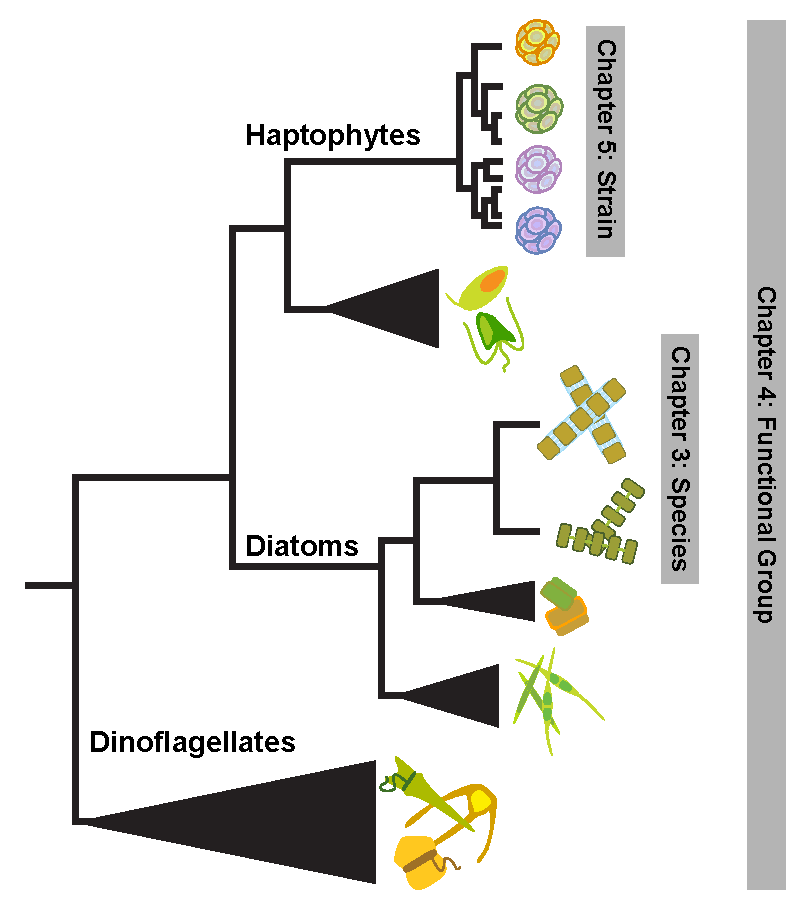
\includegraphics[width=.7\textwidth]{Images/C1_ThesisDiagram.pdf}
    \caption{Conceptual overview of the levels of diversity explored in chapters 3, 4, and 5 of this thesis.}
  \label{fig:c1f1}
\end{figure}




%% This is an example first chapter.  You should put chapter/appendix that you
%% write into a separate file, and add a line \include{yourfilename} to
%% main.tex, where `yourfilename.tex' is the name of the chapter/appendix file.
%% You can process specific files by typing their names in at the 
%% \files=
%% prompt when you run the file main.tex through LaTeX.

\chapter{Identifying reference genes with stable expression from high throughput sequence data}
\label{chap:2}
\raggedbottom
%\begin{singlespace}
%Harriet Alexander$^{1,2}$, Bethany D. Jenkins$^{3,4}$, Tatiana A. Rynearon$^{3}$, Mak A. Saito$^{5}$, Melissa L. Mercier$^{3}$, Sonya T. Dyhrman$^{2}$\\
%\\
%$^{1}$ MIT-WHOI Joint Program in Oceanography/Applied Ocean Science and Engineering, Cambridge, MA 02139, USA\\
%$^2$ Biology Department, Woods Hole Oceanographic Institution, Woods Hole, MA 02543, USA\\
%$^3$ Graduate School of Oceanography, University of Rhode Island, Narragansett, RI 02882, USA\\
%$^4$ Department of Cell and Molecular Biology, University of Rhode Island, Kingston, RI 02881, USA\\
%$^5$ Department of Marine Chemistry and Geochemistry, Woods Hole Oceanographic Institution, Woods Hole, MA 02543, USA\\
%\\
{\let\thefootnote\relax\footnotetext{This chapter was originally published as Alexander, H., Jenkins, B.D., Rynearson, T.A., Saito, M.A., Mercier, M.L., and Dyhrman, S.T. (2012). \href{http://journal.frontiersin.org/article/10.3389/fmicb.2012.00385/abstract}{Identifying reference genes with stable expression from high throughput sequence data.} \emph{Front. Microbiol.} 3, 385. }}
%\end{singlespace}
{\let\thefootnote\relax\footnotetext{H.A., B.D.J., T.A.R., M.L.M., M.A.S., and S.T.D. performed research; H.A. and S.T.D. analyzed data; H.A. and S.T.D. wrote the paper; and B.D.J., T.A.R., M.L.M., M.A.S contributed to the writing of the paper.}}
{\let\thefootnote\relax\footnotetext{The supplemental figures, tables, and data sheets for this chapter can be found in \cref{sec:app2}.}}


\clearpage

\section{Abstract}
Genes that are constitutively expressed across multiple environmental stimuli are crucial to quantifying differentially expressed genes, particularly when employing quantitative reverse transcriptase polymerase chain reaction (RT-qPCR) assays. However, the identification of these potential reference genes in non-model organisms is challenging and is often guided by expression patterns in distantly related organisms. Here, transcriptome datasets from the diatom \textit{Thalassiosira pseudonana} grown under replete, phosphorus-limited, iron-limited, and phosphorus and iron co-limited nutrient regimes were analyzed through literature-based searches for homologous reference genes, $k$-means clustering, and Analysis of Sequence Counts (ASC) to identify putative reference genes. A total of 9759 genes were identified and screened for stable expression. Literature-based searches surveyed 18 generally accepted reference genes, revealing 101 homologs in \textit{T. pseudonana} with variable expression and a wide range of mean tags per million. $K$-means analysis parsed the whole transcriptome into 15 clusters. The two most stable clusters contained 709 genes but still had distinct patterns in expression. ASC analyses identified 179 genes that were stably expressed (posterior probability, post-$p<0.1$, for 1.25 fold change). Genes known to have a stable expression pattern across the test treatments, like actin, were identified in this pool of 179 candidate genes. ASC can be employed on data without biological replicates and was more robust than the $k$-means approach in isolating genes with stable expression. The intersection of the genes identified through ASC with commonly used reference genes from the literature suggests that actin and ubiquitin ligase may be useful reference genes for \textit{T. pseudonana} and potentially other diatoms. With the wealth of transcriptome sequence data becoming available, ASC can be easily applied to transcriptome datasets from other phytoplankton to identify reference genes.
 
\section{Introduction}
Quantitative reverse transcriptase polymerase chain reaction (RT-qPCR) facilitates rapid, accurate, high-throughput analyses of gene expression, greatly enhancing and expanding molecular biological studies in a variety of organisms. This method has moved beyond the realm of model organisms \citep{Adib2004,Antonov2005, Caldwell2005, Marionneau2005, Flatt2008} to be employed for the examination of ecological and physiological characteristics of marine microbes in both culture and the environment \citep{Zehr2001, Nicot2005, Maldonado2006, Mock2008, Zhao2009, Whitney2011a, Wurch2011, Allen2008, Kustka2007, Lin2009}. There are two primary methods of gene expression analysis for single genes: 1) absolute quantification, whereby the copy number of a gene is determined through comparison of the PCR signal to a standard curve, and 2) relative gene expression, in which the expression of the gene of interest is determined through comparison to a reference gene (or internal control gene), often employing the  $2^{- \Delta \Delta CT}$ method \citep{Livak2001, Pfaffl2001, Schmittgen2008}. \par
Inherent in the $2^{- \Delta \Delta CT}$ method is the selection of a reference, or ``housekeeping,'' gene to act as an endogenous control. Ideally, the expression levels of the selected reference gene should remain stable across the treatments being examined. Genes like GAPDH, actin, and rRNA are often targeted as possible reference genes and tested for consistency in expression across treatments \citep{Vandesompele2002, Pfaffl2004, Radonic2004}. However, both \citet{Czechowski2005} and \citet{DeJonge2007a} demonstrated that canonical reference genes were often widely differentially regulated. In fact, \citet{DeJonge2007a} noted that commonly used reference genes were not represented in the fifty most stably expressed genes in the human genome. Results from RT-qPCR studies using improper reference genes (e.g. genes that are not constitutively expressed) can be significantly different from results obtained with a proper reference gene \citep{Dheda2005, Lanoix2012a}. Considering that previously established reference genes were not among the mostly stably expressed genes in model organisms, basing the selection of candidate genes for non-model organisms solely upon known reference genes may not prove the best method \citep{DeJonge2007a, Czechowski2005}. \par
	Application of RT-qPCR has proven particularly fruitful in the study of marine phytoplankton, illuminating transcriptional responses to physical stressors \citep{Rosic2010, Rosic2010}, nutrient limitation \citep{Davis2006, Moseley2006, Davis2008, Stuart2009, Whitney2011a, Wurch2011, Bender2012, Berg2008}, and the diel cycle \citep{Whitney2011a, Bender2012}, as well as highlighting the modulation and activity of many metabolic pathways \citep{Moseley2006, McGinn2008, Mock2008, Bender2012}. The success of these studies hinged upon the selection of a stably expressed reference gene. While there is often extensive literature characterizing the dynamics of suites of genes expressed under different conditions in studies of model organisms, similar breadth is lacking for non-model organisms, such as marine phytoplankton. With few genome sequences available, the selection of reference genes for eukaryotic phytoplankton is a challenge, and researchers must often choose candidate genes (e.g. actin \citep{Nicot2005}, GAPDH \citep{Czechowski2005}) based on the literature from model organisms that are distantly related to the study organism. Selecting and validating potential reference genes is a difficult task that consequently slows the development and application of targeted gene expression studies for phytoplankton. \par
	Screening the wealth of sequence data produced by modern ultra high-throughput sequencing technologies may advance and broaden the search for candidate reference genes in non-model organisms. this is particularly true of transcriptome datasets whereby genes with stable expression can be identified between treatment conditions. two statistical techniques, $k$-means clustering \citep{Hartigan1979} and analysis of sequence counts (ASC) \citep{Wu2010}, usually used to investigate patterns of differential expression in transcriptome datasets, show promise in this regard. The $k$-means algorithm is a partition-based, non-hierarchical clustering method, which divides sequence tags into the specified $k$-number of clusters, while minimizing the intra-cluster spread based on the specified distance metric \citep{Hartigan1979, Tavazoie1999, Gerstein2000, Quackenbush2001, Dhaeseleer2005}. ASC is a novel empirical Bayes method (estimating the prior distribution from the data, itself) to detect differential gene expression generated from quantifiable gene expression counts (as generated by Illumina Digital Gene Expression tag profiling, RNA-seq or similar high-throughput sequencing technologies) \citep{Wu2010}. When applied to transcriptome data these tools cannot only be used to identify genes with differential expression, they can be used to identify genes with highly stable expression patterns.\par 
	Here, literature-based searches, $k$-means clustering, and ASC are compared as tools for reference gene selection using a transcript sequence dataset collected from the centric diatom \textit{Thalassiosira pseudonana}, grown under nutrient replete, phosphorus-limited (P-limited), iron-limited (Fe-limited), and phosphorus and iron co-limited (co-limited) treatments.

\section{Materials and Methods}
\subsection{Culturing and transcriptome data collection} 
Axenic \textit{T. pseudonana} CCMP1335 was grown at $14^{\circ}$C under 24 hour light (120 $\mu$mol photons $m^{-2} s^{-1}$) after \citet{Dyhrman2012} in f/2 plus silica chelated media made from surface Sargasso Sea water. Nitrate, silica, vitamins, and trace metals were at f/2 concentrations (Guillard and Ryther 1962), while iron and phosphate were modified across treatments. In brief, triplicate cultures of replete (36 $\mu$M PO$_{4}$, 400 nM Fe), P-limited (0.4 $\mu$M PO$_{4}$, 400 nM Fe), Fe-limited (36 $\mu$M PO$_{4}$, 40 nM Fe), and co-limited (0.4 $\mu$M PO$_{4}$, 40 nM Fe) treatments were harvested when growth deviated from the replete control. Growth was monitored by cell counts. Biomass was harvested onto 0.2 $\mu$m filters and flash frozen in liquid nitrogen and total RNA was extracted as described in \citep{Dyhrman2012}. Tag-seq sequencing of the transcriptome was performed by Illumina with a polyA selection and NlaIII digestion, resulting in $21$ base pair sequence reads or tags \citep{Dyhrman2012}. Libraries were of varied sizes as follows: replete ($\sim$12 million), P-limited ($\sim$13 million), Fe-limited ($\sim$23 million), and co-limited ($\sim$26 million). Tags were mapped to gene models (predicted protein coding regions) with a pipeline designed by Genesifter Inc., requiring 100\% identity and covering 9759 genes. Tag counts within a gene were pooled and normalized to the size of the library, with resulting data expressed in tags per million (TPM). Genes with normalized tag counts less than 2.5 TPM for each of the four treatments were excluded (\cref{fig:a1f1}), leaving 7380 genes in the analysis. The data discussed in this publication have been deposited in NCBI Gene Expression Omnibus (GEO) (Edgar, 2002) and are accessible through GEO Series accession number \href{http://www.ncbi.nlm.nih.gov/geo/query/acc.cgi?acc=GSE40509}{GSE40509}.  
\subsection{Reference gene identification}
\par The current, relevant literature from algae and plant-based studies was queried for reference genes used as endogenous controls for relative gene expression assays. Stably expressed genes reported in the literature were compared using BLASTn \citep{Altschul1997} against the \textit{T. pseudonana} genome in NCBI (AAFD00000000.2) to find homologs (e-value $< 1.0$e-1). A loose e-value cutoff was used to be inclusive and enhance our collection of all potential reference gene candidates. In addition, the Eukaryotic Orthologous Group (KOG) definitions for the genes found via BLAST were identified, and subsequent genes located in the KOG definition families were included in the analysis.\par 
For the $k$-means analysis, tag counts from the four treatments corresponding to the 7380 genes with reads greater than 2.5 TPM were clustered using the $k$-means algorithm under the Pearson correlation coefficient. The distance was measured with a Pearson correlation as it has been found to perform as well or better than other similar distance measures for non-ratio or count-based data \citep{Gibbons2002}, such as the \textit{T. pseudonana} transcriptome dataset. The number of clusters ($k$) was determined via a figure of merit (FOM) estimation, which is an approximation of the predictive power of the clustering method \citep{Yeung2001}. FOM analysis was performed by predicting the FOM value for values of $k$ ranging from $k=1$ (one cluster) to $k=50$ (fifty clusters). The FOM value decreases as the within-cluster similarity increases, thus the FOM value was minimized to determine the optimal $k$-value. All clustering analyses were performed using the MultiExperiment Viewer (MeV) version 4.7 \citep{Saeed2003, Saeed2006}. Possible reference gene targets were identified by isolating clusters of genes that exhibited similarly stable expression patterns across the four treatments. \par
Using ASC \citep{Wu2010}, the statistical significance of an observed fold change was determined in pairwise comparisons between each of the limited treatments and the replete control. The posterior probability (post-$p$) was calculated by computing the posterior mean of the log ratio of proportions over each of the P-limited, Fe-limited, and co-limited treatments relative to the replete treatment for a fold change of 1.10, 1.25, and 1.50. Possible constitutively expressed genes were identified by selecting genes for which the post-p of each of the nutrient-limited treatments relative to the replete treatment for each of the fold change values was less than a specified cutoff. Posterior probability cutoffs between 0.01 and 0.20 were assessed across each of the fold changes (\cref{tab:c2t1}). Ultimately, a post-$p$ of 0.10 was selected for further analyses (meaning that genes selected had less than a 10\% chance of having the specified fold change between treatments), for it yielded genes across all of the fold change bins examined and demonstrated a broader range of mean normalized tag counts than seen for a post-$p$ of 0.05 or 0.01. All ASC analyses were made using ASC $0.1.5$ in \href{http://R-project.org}{R}. \par

\section{Results}
Transcript sequence data was generated from \textit{T. pseudonana} CCMP1335, grown in four different treatments (replete, P-limited, Fe-limited, and co-limited). Potential reference genes were identified through 1) querying the data to identify expression of common reference genes based on literature searches, 2) a pattern-driven analysis using $k$-means clustering \citep{Hartigan1979} and 3) a quantitative analysis based the probability of fold change using ASC. \par
Selection of reference genes often falls upon those used in previous relative expression studies. The literature was surveyed for RT-qPCR expression studies employing the $2^{- \Delta \Delta CT}$ method for the following algae and plants: \textit{T. pseudonana} \citep{Maldonado2006, McGinn2008, McGinn2008a, Mock2008, Park2008, Carvalho2011, Whitney2011a}, \textit{Thalassiosira weissflogii} \citep{Davis2006, McGinn2008, Park2008, Whitney2011a}, \textit{Phaeodactylum tricornutum} \citep{Siaut2007, McGinn2008}, \textit{Emiliana huxleyi} \citep{Bruhn2010, Richier2011}, \textit{Micromonas pusilla} \citep{McDonald2010}, \textit{Chlamydomonas reinhardtii} \citep{Moseley2006, Zhao2009}, \textit{Alexandrium} spp. \citep{Lee2009, Moustafa2010}, \textit{Symbiodinium} sp. \citep{Rosic2010, Rosic2010a, Leggat2011}, \textit{Prorocentrum minimum} \citep{Guo2012}, \textit{Aureococcus anophagefferens} \citep{Berg2008, Wurch2011}, \textit{Solanum tuberosum} \citep{Nicot2005}, and \textit{Arabidopsis thaliana} \citep{Avonce2004}. Results from the current literature survey yielded a list of 18 key reference genes frequently employed in the study of gene expression for eukaryotic phytoplankton and plants: actin, calmodulin, cyclin dependent kinase, cyclophilin, cytochrome c, G-protein beta subunit, ferric enterobactin binding periplasmic protein precursor, histones, elongation factors, GAPDH, heat shock protein 90, poly(A) polymerase, ribosomal protein large subunit, ribosomal protein small subunit, SAM, $\alpha$-, $\beta$-, $\gamma$-tubulin, and ubiquitin conjugating enzymes (\ref{DS21}). It is important to note that as more reference genes are validated as stable, the selection of putative reference genes may expand. The 101 genes identified as homologous to these reference genes across the four treatments in \textit{T. pseudonana} had variable expression patterns and a wide range of mean normalized counts (0.08 to 1087.8 TPM) (\cref{fig:c2f1}). Genes within a specific gene family (e.g. the five actin genes) had different mean counts as well as variable coefficients of variation (CV), which is indicative of variable expression (\ref{DS21}). For example, ACT 1 (NCBI: 7449411) had a mean expression of 1024.1 TPM and a CV of only 12.3\%, where as ACT 5 (NCBI: 7445819) had a lower mean expression of 23.95 and a higher CV of 35.5\% (\ref{DS21}). \par

%Figure 1: Expression across treamtments
\begin{figure}[p!]
  \centering
    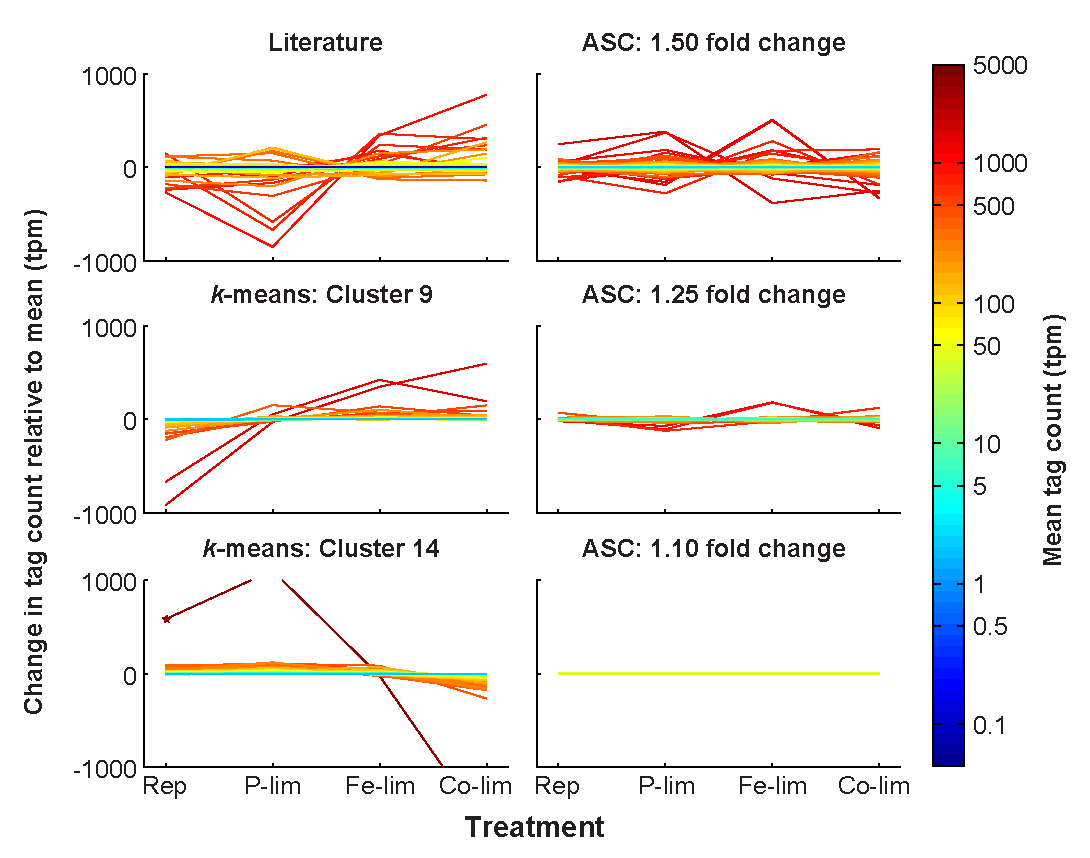
\includegraphics[width=1\textwidth]{Images/C2_Figure1_v6.pdf}
    \caption[Expression patterns of putative reference genes]{Expression patterns of putative reference genes identified through literature-based searches, $k$-means clustering, and ASC analysis. Through literature-based searches, a total of 101 genes homologous to reference genes from previous studies on plants and algae were identified in \textit{T. pseudonana} and plotted to indicate deviation and mean TPM (Literature). $K$-means clustering was applied to the 7380 genes and Cluster 9 (243 genes) and Cluster 14 (466 genes) possessed the genes with the most stable expression pattern across the four treatments. Genes from these clusters are plotted to indicate deviation and mean TPM ($k$-means: Cluster 9; $k-$means: Cluster 14). ASC was used to assess statistical significance (post-$p < 0.1$) of fold changes of 1.10, 1.25, and 1.50 for each treatment relative to the replete control. Genes from these fold change bins are plotted to indicate deviation and mean TPM (ASC: 1.50 fold change; ASC: 1.25 fold change; ASC 1.10 fold change). For a fold change of 1.10, two genes, both hypothetical proteins, (NCBI: 7446346 and 7452192) passed the post-$p < 0.1$ cutoff, and represent the most stable genes based on the ASC analysis (\ref{DS23}). For each of the six classes of putative reference genes, tag counts were normalized to total library size (in TPM) and are plotted relative to the mean for each of the four treatments: Replete (Rep), P-limited (P-lim), Fe-limited (Fe-lim), and co-limited (Co-lim). The color of the line correlates to the mean normalized tag count. A star marks a gene (NCBI: 7451632) in Cluster 14 that is not on the scale of expression for P-limited (1104.7 TPM) and co-limited (-1664.9 TPM) treatments. }
  \label{fig:c2f1}
\end{figure}

The high-throughput transcript dataset was analyzed with $k$-means clustering. Prior to performing $k$-means cluster analysis, FOM optimization was run and found to be minimized at $k=1$5. Thus, $k$-means analysis was run under the Pearson correlation coefficient for $k=15$, yielding 15 clusters, for which the intra-cluster variation was minimized (\cref{fig:a1f2}). Of the 15 clusters produced (ranging in size from 162 to 954 genes), Cluster 4 (433 genes), Cluster 9 (243 genes), and Cluster 14 (466 genes) had candidate reference genes based on a low magnitude of change associated with the expression patterns in those clusters (\cref{fig:a1f2}). However, Cluster 4 showed a clear pattern of differential regulation (downregulated in the replete and upregulated in the co-limited), and as such it was not considered to be an optimal candidate cluster and was excluded from additional analyses. Both Cluster 9 and Cluster 14 consisted of genes with a wide range in mean TPM values (1.74 to 4191.91 TPM), with relatively small deviations from the mean value (\cref{fig:c2f1}; \ref{DS22}), which stands in contrast to other clusters that had definite treatment driven expression patterns (\cref{fig:a1f2}). Despite the relatively small deviations from the mean value, genes in Clusters 9 and 14 displayed both clear patterns of regulation, as demonstrated by the average change in tag count relative to the mean (\cref{fig:c2f2}) and the presence of ``outlier'' genes with differential expression such as NCBI: 7451632, which was downregulated in the co-limited treatment for Cluster 14 (\cref{fig:c2f1}; \ref{DS22}). \par

%Figure 2: Deviation from the mean
\begin{figure}[h!]
  \centering
    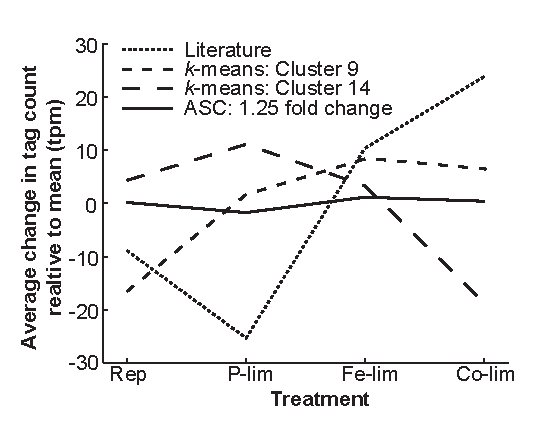
\includegraphics[width=0.65\textwidth]{Images/C2_Figure2_v6.pdf}
    \caption[Average deviation from the mean level of expression for putative reference genes]{Average deviation from the mean level of expression for all genes found with literature-based searches, $k$-means clustering, and ASC analysis of 1.25 fold change. The average change in tag count from the mean expression (TPM) for all the genes identified through literature-based searches for genes homologous to known reference genes from the literature $(n = 101)$, $k$-means clustering from Cluster 9 $(n = 243)$ and Cluster 14 (n = 466), and ASC analysis identifying genes demonstrating a 1.25 fold change with a post-$p < 0.1$ $(n = 179)$. The mean standard deviations for the four cases are as follows: Literature (92.62 TPM), Cluster 9 (41.66 TPM), Cluster 14 (43.12 TPM), and ASC (14.24 TPM). The mean TPM is plotted for the four treatments: Replete (Rep), P-limited (P-lim), Fe-limited (Fe-lim), and co-limited (Co-lim).}
  \label{fig:c2f2}
\end{figure}

Adapting ASC to examine stable expression patterns, genes for which the post-$p$ was less than 0.1 (e.g. had less than a 10\% chance of equaling or exceeding the fold change cutoff) were plotted in three low fold change bins: 1.10, 1.25, and 1.50. A post-$p$ of 0.1 was selected as it optimized the dataset for a wide range of mean gene expression values and provided coverage for each of the fold change bins examined (\cref{tab:c2t1}). The number of genes in each of the fold change bins increased with increasing value of fold change. For example, two genes passed the 1.10 cutoff, 179 genes passed the 1.25 cutoff, and 1375 genes passed the 1.50 cutoff. With the increase in the number of genes came an increase in the variation from the mean of the normalized tag counts (\cref{fig:c2f1}; \ref{DS23}). \par
The bin with the 1.10 cutoff had two genes (NCBI: 7446346 and 7452192), which are both hypothetical proteins (\cref{fig:c2f1}). A BLASTn search of 7446346 against the nr NCBI database yielded 69\% identity over 251 base pairs (e-value, 1e-13) to a hypothetical protein (NCBI: CP000544.1) from \textit{Halorhodospira halophila}, a salt-tolerant purple bacterium, and 69\% identity over 232 base pairs (e-value, 1e-12) to a hypothetical protein (NCBI: CP001905.1) from \textit{Thioalkalivibrio} sp. K90mix, also a salt-tolerant chemolithoautotrophic bacteria. BLASTp searches of 7452192 showed the highest identity hits to hypothetical proteins from \textit{Aureococcus anophagefferens} (NCBI: EGB11506.1; 31\% identity; e-value, 2e-21) and from \textit{Chlorella variablis} (NCBI: EFN56803.1; 24\% identity; e-value, 7e-11).\par




The 1.25 fold change bin was used for the identification of candidate reference genes as it offered a larger selection than the 1.10 fold change bin without including genes with increased deviations from the mean, as was the case with the 1.50 fold change bin. Thus, the 1.25 fold change category was the focus of the rest of the analyses (\ref{DS23}). Genes in the 1.25 fold change bin showed a broad range of mean normalized tag counts ranging from 7 to over 1200 TPM with a median of 41.94 TPM, providing for the selection of genes with different levels of constitutive expression in the cell (\cref{fig:c2f1}). Notably, the median of the average tag counts of the genes in the ASC 1.25 fold change bin was 41.94 TPM, which is much higher than that of both Cluster 9 and Cluster 14 with median values of 14.18 TPM and 21.93 TPM, respectively. \par

\begin{landscape}
\begin{table}[h!]
\centering
\caption{Gene counts for the fold change bins of 1.50, 1.25, and 1.10 across posterior probability cutoffs ranging from 0.01 to 0.20.}
\label{tab:c2t1}
\small
\begin{tabular}{|p{2.2cm}|p{1.25cm}|p{1.25cm}|p{1.25cm}|p{1.25cm}|p{1.25cm}|p{1.25cm}|p{1.25cm}|p{1.25cm}|p{1.25cm}|}
\hline
Fold change & \multicolumn{3}{c|}{1.50}                   & \multicolumn{3}{c|}{1.25}                   & \multicolumn{3}{c|}{1.10}                   \\ \cline{1-10} 
Posterior probability                             & Number of genes & Min. TPM & Max. TPM & Number of genes & Min. TPM & Max. TPM & Number of genes & Min. TPM & Max. TPM \\ \hline
post-$p < 0.2$        & 1649            & 2.11        & 1802.38     & 312             & 2.83        & 1281.15     & 8               & 20          & 176.63      \\ \hline
post-$p < 0.1$         & 1375            & 2.22        & 1802.38     & 179             & 7.06        & 1281.15     & 2               & 51.81       & 105.73      \\ \hline
post-$p < 0.05$       & 1127            & 2.83        & 1802.38     & 122             & 20          & 1281.15     & 1               & 105.73      & 105.73      \\ \hline
post-$p < 0.01$        & 801             & 5.69        & 1802.38     & 62              & 20          & 1281.15     & 0               & NA          & NA          \\ \hline
\end{tabular}
\end{table}
\end{landscape}



	Underlying differences in the magnitude and pattern of expression variation across treatments were identified by examining the average tag count change for each reference gene detection method (\cref{fig:c2f2}). If all genes in a group were perfectly constitutively expressed, the average change in tag count relative to the mean observed would be 0 TPM (e.g. the TPM values across all treatments for each of the genes within a group were the same). The average variation from the mean observed in the literature (ranging from -25.34 to 23.84 TPM) highlighted the differential expression across treatments. The average change in tag count relative to the mean in both Cluster 9 (ranging from -16.56 to 8.47) and Cluster 14 (ranging from -18.72 to 11.11 TPM) clearly demonstrated patterns of regulation across treatments (e.g. the upregulation under P-limitation and downregulation under co-limited observed in Cluster 14). In contrast, the average change in tag count relative to the mean observed in the genes identified through ASC (1.25 fold change with post-$p$ < 0.1), which showed a low magnitude of variation (ranging from -1.732 to 1.613 TPM) and a small mean standard deviation across the four treatments (14.24 TPM). Ultimately, the expression patterns of the majority of the genes identified through literature-based searches and $k$-means clustering were more variable across the \textit{T. pseudonana} test treatments, than those genes identified with ASC.\par	
\begin{figure}[h!]
  \centering
    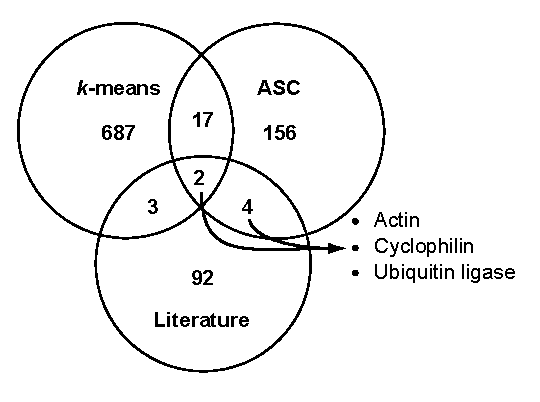
\includegraphics[width=0.75\textwidth]{Images/C2_Figure3_v6_bw.pdf}
    \caption[Comparison of putative reference genes identified through literature, $k$-means clustering, and ASC analysis]{Comparison of possible reference genes found with literature-based searches, $k$-means clustering, and ASC analysis of 1.25 fold change. Venn diagram analysis was used to compare genes identified as candidate reference genes through literature-based homolog searches (totaling 101 genes), with the $k$-means clustering method (genes in Cluster 9 and 14, totaling 709 genes), and with quantitative exclusion by ASC (based on genes demonstrating a 1.25 fold change with a post-$p < 0.1$, totaling 179 genes). The number of genes in each region is reported. The intersection of all ASC and literature-based searches yielded six total genes representing three different gene families: actin (NCBI: 7449411), cyclophilin (NCBI: 7445376), and ubiquitin ligase (NCBI: 7448637, 7450639, 7446724, and 7451971). }
  \label{fig:c2f3}
\end{figure} 
A comparison of the three techniques: literature-based searches, $k$-means cluster selection, and ASC cutoff at 1.25 fold change revealed comparatively few genes in common between the techniques (\cref{fig:c2f3}). Of the 709 genes identified through $k$-means clustering and the 179 genes found through ASC analysis (genes which pass the 1.25 fold change cutoff for post-$p$ < 0.1), 21 genes are shared (\cref{fig:c2f3}), of which six lacked GO annotations or KOG definitions (\ref{DS22}). Between the genes identified through literature and ASC analysis, six genes were held in common; these genes were representative of the general gene classifications: actin (NCBI: 7449411), cyclophilin (NCBI: 7445376), and ubiquitin ligases (NCBI: 7448637, 7450639, 7446724, and 7451971). Only two genes (NCBI: 7448637 and 7446724) were found in common amongst all three methods of reference gene selection, both of which were annotated as putative ubiquitin ligases (\ref{DS21}). \par



\section{Discussion}
	Prior to the availability of high-throughput molecular datasets, reference genes for non-model organisms were selected based on literature reports of stably expressed genes in model organisms. With non-model organisms such as eukaryotic phytoplankton this task is particularly difficult, as stably expressed genes are not readily apparent in the relatively limited molecular literature specific to these organisms. Often the selection of a reference gene relies on information from distantly related organisms under dissimilar conditions, leading to extensive validation work \citep{McDonald2010, Whitney2011a}. Herein, we compared the efficacy of reference gene selection based on the literature as compared to verifiable selection through $k$-means clustering and ASC analysis of high-throughput transcriptome data in \textit{T. pseudonana} across four nutrient treatments (replete, P-limited, Fe-limited, and co-limited). These treatments are of environmental relevance as both P and Fe are major drivers of diatom physiological ecology and consequently carbon fixation \citep{Moore2004}. Additionally, P and Fe often occur concurrently at very low concentrations in marine systems and have been found to be independently co-limited, or mutually exclusive biochemically \citep{Saito2008}.\par
    Our literature-based search of relative gene expression studies from 12 algae and plants yielded 18 general reference gene categories, for which 101 homologs in the \textit{T. pseudonana} genome were identified (\ref{DS21}). While some of these genes demonstrated stable expression (e.g. actin, cyclophilin, and ubiquitin conjugating enzymes), the vast majority displayed some form of differential expression in the treatments examined herein. Furthermore, there was considerable heterogeneity of expression among the different gene copies of actin, cyclophilin, and ubiquitin conjugating enzymes, demonstrating that not all genes within a gene family are stably expressed. These data underscore that a literature-based selection of reference genes necessitates validation across all treatments of interest \citep{Vandesompele2002, Pfaffl2004}. \par
	Differential expression patterns in high-throughput datasets are often analyzed with clustering methods, such as hierarchical or $k$-means clustering \citep{Dhaeseleer2005}. Rather than using a clustering method for the identification of differential expression patterns, here it is applied to identify constitutively expressed genes. The $k$-means clustering algorithm was chosen as it is a top-down or partition-based approach to gene clustering that is not hierarchical and requires few assumptions about the data \citep{Hartigan1979}. Several of the 709 putative reference genes identified by $k$-means analysis (from Clusters 9 and 14) were clearly differentially regulated, with large deviations from the mean expression level. The presence of outliers is to be expected using the $k$-means method, for it is a pattern-based method and all genes must be placed into one of the partitioned $k = 15$ clusters. Thus, optimal placement of a gene is not always guaranteed. As with a finite number of clusters, the assignment of a gene is often forced. For example, even genes in Cluster 9 and 14 were subject to strong patterns of regulation, with both clusters demonstrating large average changes in tag count relative to the mean tag count. Arguably, it is better to select a reference gene from a pool of genes that do not share the same pattern of regulation. Therefore, genes uncovered via $k$-means clustering must be manually surveyed to exclude genes with large deviation prior to the selection of a candidate reference gene.\par
	In lieu of clustering approaches, other studies have used statistical parsing of ESTs in tomato plants \citep{Coker2003} and Affymetrix whole-genome GeneChip data from \textit{A. thaliana} \citep{Czechowski2005} and humans \citep{DeJonge2007a} to identify reference genes that have small deviations from the mean of replicated treatments. In contrast to these and other statistical methodologies typically applied to high-throughput sequence data with replication, the Bayesian approach to gene expression analysis, ASC, allowed for selection of candidate genes based on a statistical cutoff rather than cardinality. Though typically used for the identification of differentially expressed genes, the function of ASC was reversed in this study by lowering the post-$p$ cutoff. Genes for which post-$p < 0.1$ for a specified fold change were targeted, meaning that genes that were unlikely to have made that fold change were selected. The 1.25 fold change bin yielded the most options for candidate reference genes without sacrificing stability of expression (as was seen in the 1.50 fold change bin). \par
	ASC provides a method of identifying reference genes with expression levels similar to those of target genes. For example, the mean normalized tag counts of genes identified using ASC were broad (from 7 to over 1200 TPM), providing the opportunity for reference gene expression to be generally matched with target gene expression. Current studies frequently employ reference genes for endogenous control that have very high levels of expression across all treatments, such as ACT1 (NCBI: 7449411) in \textit{T. pseudonana} (which has a mean expression value of 1024.1 TPM in this data set), yet these highly expressed genes might not be optimal for studies of genes with low levels of expression or when multiplexing targets in probe-based RT-qPCR analysis. \par
	High-throughput transcript datasets also allow the selection of reference genes to move beyond the confines of gene annotation and previously identified reference genes. In fact, the two genes with the most stable expression in the 1.10 fold change bin are hypothetical, with no clear annotation. Of the 179 genes that passed the 1.25 fold change cutoff with ASC, 44 lacked both GO and KOG annotations. A large percentage of the 11,390 genes in the \textit{T. pseudonana} genome are annotated as hypothetical proteins \citep{Armbrust2004, Mock2008}, and here we show a number of them are stably expressed across the target conditions. This has been seen with model organisms, where a good majority of constitutively expressed genes fall outside the bounds of preconceived ``housekeeping'' genes \citep{Czechowski2005, DeJonge2007a}. By using a Bayesian approach such as ASC, hypothetical proteins can be chosen as reference genes. \par
    Comparison of the putative reference genes recovered using ASC to previous studies served to cross-validate the ASC approach. Actin (ACT1, NCBI: 7449411) has been validated in the literature as a suitable reference gene for relative expression studies of \textit{T. pseudonana} under Fe-limitation \citep{Whitney2011a}, a treatment considered in this study, and was one of the 179 genes passing the ASC 1.25 fold change cutoff. Additionally, only five of the 179 genes with stable expression found with ASC were identified as differentially expressed in a study of \textit{T. pseudonana} under additional treatments to those described here (e.g. nitrogen limitation, silica limitation, etc.) \citep{Mock2008} (\ref{DS24}). Of the five, only one gene (NCBI: 7451974) was identified as differentially expressed under Fe-limitation, a condition examined in this study. Taken together, this validates the genes identified with ASC using alternative data and methods, and suggests that the ASC-detected genes are globally stable across many different conditions for \textit{T. pseudonana}. However, one of the two genes identified in the 1.10 fold change bin (NCBI: 7446346) was identified as significantly down-regulated under nitrogen limitation by \citet{Mock2008}. This highlights the importance of validating genes across all treatments of interest prior to their use as reference genes. \par
	Notably, the $k$-means and ASC dataset revealed only 21 genes in common. The 179 genes found through ASC were, in fact, distributed fairly evenly across all of the 15 clusters. The lack of intersection observed between the two datasets is likely related to the parsing ability inherent in $k$-means clustering. The $k$-means approach is highly driven by patterns of differential regulation, but does not consider the significance of that regulation (e.g. genes that are not significantly upregulated are placed in a cluster with genes that are significantly upregulated). Thus, the stably expressed genes that were identified by ASC, though not displaying major patterns of regulation, were clustered based on minor patterns in variation of gene expression. Therefore, while $k$-means clustering provides a global view of commonalities in gene expression patterns, ASC is more robust at identifying reference genes.\par
	Eight genes were common between the ASC and literature-based searches, which were distributed across three general gene classes: actin (NCBI: 7449411), cyclophilin (NCBI: 7445376), and ubiquitin ligases (NCBI: 7448637, 7450639, 7446724, and 7451971). For those interested in identifying suitable reference genes for studies in \textit{T. pseudonana} but lack transcriptome datasets across the treatments of interest, these eight genes may serve as good tentative reference genes as they are verified in this study and have been identified as stable in many other organisms under many conditions. In particular, ubiquitin ligases/conjugating enzymes have been used as reference genes in several studies involving other algae, namely, \textit{Aureococcus anophagefferens}, \textit{Phaeodactylum tricornutum}, and \textit{Prorocentrum minimum} \citep{Siaut2007, McGinn2008, Guo2012, Wurch2011, Berg2008}, and with further analysis may represent particularly good reference genes in the phytoplankton. \par
	Sequence-based transcriptome profiling has become an increasingly useful method for gene discovery and differential expression analysis. Yet, RT-qPCR is still valuable for the examination of detailed trends in expression in both culture and field studies. Here we show that the application of ASC and, to a lesser extent, $k$-means clustering can be used to successfully screen transcriptome data for potential reference genes. The isolation of candidate reference genes using ASC with the 1.25 fold change cutoff for post-$p < 0.1$ was more robust and stringent at excluding differentially expressed genes than both the literature-based searches and $k$-means clustering. Based on these data for \textit{T. pseudonana}, it was shown that ACT 1 and ubiquitin ligase may be useful reference genes. Yet, in addition to these common reference genes, the data demonstrate that there are many more stably expressed genes (both annotated and hypothetical) to choose from for expression studies in this and potentially other diatoms. Notably, this survey focused only on variation in P and Fe supply, so these genes may not transfer to studies of other nutritional drivers or other physical forces, such as light intensity or temperature. As more transcriptome data are generated for phytoplankton, ASC can be employed without sequence replicates, to identify reference genes for other phytoplankton under various conditions. Additionally, the suite of genes identified through these analyses might allow for better multi-gene normalization analysis that would provide for the detection of smaller fold changes with certainty \citep{Vandesompele2002, Czechowski2005}.\par




%% This is an example first chapter.  You should put chapter/appendix that you
%% write into a separate file, and add a line \include{yourfilename} to
%% main.tex, where `yourfilename.tex' is the name of the chapter/appendix file.
%% You can process specific files by typing their names in at the 
%% \files=
%% prompt when you run the file main.tex through LaTeX.

\chapter{Integrating archival tag data and a high-resolution oceanographic model to estimate basking shark (\textit{Cetorhinus maximus}) movements in the western Atlantic}
\label{chap:3}
\raggedbottom
%\begin{singlespace}
%Camrin D. Braun1,2*, Gregory B. Skomal3, Simon R. Thorrold2
	%Massachusetts Institute of Technology-Woods Hole Oceanographic Institution Joint Program in %Oceanography/Applied Ocean Science and Engineering, Cambridge, MA 02139
	%Biology Department, Woods Hole Oceanographic Institution, Woods Hole, MA 02540
	%Massachusetts Division of Marine Fisheries, New Bedford, MA 02744, USA

%*corresponding author: cbraun@whoi.edu; +1 5082893961
%Keywords: movement ecology; satellite archival telemetry; migration; mesopelagic; oceanographic modeling; %site fidelity


%\\
{\let\thefootnote\relax\footnotetext{This chapter was originally published as Braun, C.D., Skomal, G.B., and Thorrold S.R. (2018). \href{https://www.frontiersin.org/articles/10.3389/fmars.2018.00025/full}{Integrating archival tag data and a high-resolution oceanographic model to estimate basking shark (\textit{Cetorhinus maximus}) movements in the western Atlantic.} \emph{Fron. Mar. Sci.} 5: 25. }}
%\end{singlespace}
{\let\thefootnote\relax\footnotetext{G.B.S. and S.R.T. designed the study and conducted the tagging; C.D.B. performed the analysis and wrote the paper. G.B.S. and S.R.T. contributed to the writing of the paper.}}
{\let\thefootnote\relax\footnotetext{The supplemental figures, tables, and data sheets for this chapter can be found in \cref{sec:app3}.}}

\clearpage

\section{Abstract}

Basking shark (\textit{Cetorhinus maximus}) populations are considered ‘vulnerable’ globally and ‘endangered’ in the northeast Atlantic by the International Union for the Conservation of Nature. Much of our knowledge of this species comes from surface observations in coastal waters, yet recent evidence suggests the majority of their lives may be spent in the deep ocean. Depth preferences of basking sharks have significantly limited movement studies that used pop-up satellite archival transmitting (PSAT) tags as conventional light-based geolocation is impossible for tagged animals that spend significant time below the photic zone. We tagged 57 basking sharks with PSAT tags in the NW Atlantic from 2004-2011. Many individuals spent several months at meso- and bathy-pelagic depths where accurate light-level geolocation was impossible during fall, winter and spring. We applied a newly-developed geolocation approach for the PSAT data by comparing three-dimensional depth-temperature profile data recorded by the tags to modeled in-situ oceanographic data from the high-resolution HYbrid Coordinate Ocean Model (HYCOM). Observation-based likelihoods were leveraged within a state-space hidden Markov model (HMM). The combined tracks revealed that basking sharks moved from waters around Cape Cod, MA to as far as the SE coast of Brazil (20$^{\circ}$ S), a total distance of over 17,000km. Moreover, 59\% of tagged individuals with sufficient deployment durations (> 250 days) demonstrated seasonal fidelity to Cape Cod and the Gulf of Maine, with one individual returning to within 60 km of its tagging location one year later. Tagged sharks spent most of their time at epipelagic depths during summer months around Cape Cod and in the Gulf of Maine. During winter months, sharks spent extended periods at depths of at least 600 m while moving south to the Sargasso Sea, the Caribbean Sea, or the western tropical Atlantic. Our work demonstrates the utility of applying advances in oceanographic modeling to understanding habitat use of highly migratory, often meso- and bathy-pelagic, ocean megafauna. The large-scale movement patterns of tagged sharks highlight the need for international cooperation when designing and implementing conservation strategies to ensure that the species recovers from the historical effects of over-fishing throughout the North Atlantic Ocean.

\section{Introduction}
The basking shark, \textit{Cetorhinus maximus} (Gunnerus 1765), is the second largest fish species, attaining weights of up to 4 tonnes and lengths up to 12 m \citep{Sims2008}. It is known to inhabit boreal to tropical \citep{Skomal2009} waters circumglobally and is most often observed on continental shelves \citep{Sims2006}. Despite its size and widespread distribution, major gaps in our understanding of basking shark ecology remain. Population size and structure are currently unresolved and information about fisheries interactions is limited \citep{Sims2008}. Although there is evidence to suggest population recovery in some areas following exploitation \citep{Witt2012}, the lack of information about key life history traits, population size, movements, and habitat use is problematic as global anthropogenic pressures on elasmobranchs continue to rise \citep{Dulvy2008, Ferretti2010}.

Basking sharks exhibit life history characteristics that make them particularly vulnerable to exploitation, including low fecundity, slow growth and maturity, and long gestation times \citep{Compagno1984, Sims2008}. There is, therefore, concern over the status of basking shark populations worldwide, and the species is listed on Appendix II of the Convention on the International Trade in Endangered Species (CITES) and Appendices I and II of the Convention for the Conservation of Migratory Species of Wild Animals (CMS). It is also considered ‘vulnerable’ globally and 'endangered' in the northeast Atlantic by the International Union for the Conservation of Nature (IUCN).

Historically, information on the ecology of large pelagic animals has been limited to scarce observations that are limited geographically \citep{Templeman1963, Squire1990, Francis2002}. Almost all of our knowledge of basking shark ecology, for instance, comes from surface observations in coastal waters \citep{Sims2006, Sims2008}.  Yet recent evidence from electronic archival tags suggests that perhaps the majority of their lives are spent offshore at depths below the euphotic zone \citep{Skomal2009}. Indeed, the rapid development of electronic tag technologies has provided a powerful means of gaining detailed information about the behavior of marine species \citep{Block2011}. PSAT tags have been particularly helpful in ocean environments as data are relayed back to the researcher via satellite upon tag release from the individual \citep[\emph{e.g.}][]{Block2011}. These tags have provided a wealth of information on sharks \citep{Werry2014, Berumen2014}, rays \citep{Braun2014, Thorrold2014a}, and large teleost fishes \citep{Braun2015a} by eliminating the need to physically recover the tag at the end of the deployment. 

While electronic tags have revolutionized the study of movement ecology in the ocean, a significant hurdle remains when attempting to track marine fishes compared with terrestrial counterparts.  Tags using Argos or Global Positioning System (GPS) locations require the tag antenna to break the water surface long enough for communication with satellites to be established (Argos) or a snapshot of the satellite constellation to be received (GPS). Researchers, have, therefore, relied mostly on PSAT tags that use light-level geolocation in which a threshold algorithm is used to detect solar altitude above the horizon from which estimates of longitude (local noon) and latitude (sunrise/sunset) can be estimated \citep{Hill2001}. While sea surface temperature (SST) and bathymetry can improve these estimates \citep{Galuardi2010, Lam2010}, light-based geolocation requires occupation of the photic zone to record adequate light data for geolocation, and even estimates with quality light data can be error prone \citep{Braun2015}.  However a number of marine species rarely, if ever, experience enough downwelling light or spend adequate time at the surface to determine their position with PSAT tags \citep{Aarestrup2009, Skomal2009, Peklova2012}. Animals that spend significant time at depths below the photic zone have, therefore, proved extremely difficult to track in ocean ecosystems \citep[\emph{e.g.}][]{Skomal2009, Dewar2011}. 

The use of PSAT tags to track basking shark movements has proved particularly difficult in the northwestern Atlantic as basking sharks spend months at a time below the euphotic zone where light-based geolocation is impossible \citep{Skomal2009}.  We have recently developed a new geolocation approach that combines all the physical data collected from archival tags, including light levels and depth-temperature profiles, in a likelihood framework to more accurately track the movements of tagged fishes in the ocean \citep{Braun2018a}. Our method uses a purely diffusive animal movement model (\emph{e.g.} Brownian motion) with behavior state switching (migratory or resident states based on a priori movement speeds) coupled with observations of the environment (\emph{e.g.} in situ or modeled oceanography) to estimate the posterior distribution of the state (\emph{e.g.} animal position and behavior) in a hidden Markov model (HMM) framework. Depth-temperature profiles provide diagnostic oceanographic signatures that, along with other data sources like light, SST, and maximum depth, may be leveraged to help constrain position \citep{Aarestrup2009, Skomal2009}.

Satellite tags have been deployed on basking sharks in the Atlantic since the pioneering work of \cite{Priede1984}. Yet, basking shark movements and ecology remain poorly understood. Here, we present the results of an intensive tagging effort that deployed 57 PSAT tags on adult basking sharks during summer months in waters adjacent to Cape Cod, Massachusetts. Profiles recorded by the tags were integrated with high-resolution oceanographic model outputs and in situ climatological data to construct likelihoods and improve geolocation estimates for basking sharks. The data provide a rare assessment of the large-scale movements and migratory behavior of the ocean’s second largest fish.  The information is, in turn, a prerequisite for any attempts to estimate abundance and population structure of basking sharks in the Atlantic Ocean.

\section{Methods}
\subsection{Study area and tagging}
We opportunistically deployed a variety of PSAT tags on basking sharks near Cape Cod, Massachusetts (USA) in the Northwest Atlantic (NWA) between 2004 and 2011 (\cref{fig:c3t1}). Total length of each individual was estimated relative to the tagging vessel and, where possible, the pelvic region was visually inspected to determine sex. Tags were applied by a professional harpoon fisherman into the dorsal musculature near the base of the first dorsal fin \citep{Chaprales1998}. This research was performed in accordance with the Woods Hole Oceanographic Institution’s Animal Care and Use Committee (IACUC) protocol #16518.

\subsection{Tag types}
Three types of PSAT tags were deployed on basking sharks (\cref{fig:c3t1}). These tags (Models Mk10-PAT, Mk10-AF, miniPAT; Wildlife Computers, Inc., WA, USA) logged depth, temperature, and light level data every 10 seconds (Mk10-AF) or 15 seconds (Mk10-PAT, miniPAT) to onboard memory. All tags recorded light data for geolocation purposes, and the Mk10-AF tag housed a Fastloc GPS receiver for acquiring high-resolution location information. Software in the tags summarized the high-resolution archived data into depth-temperature profiles at 8 depths (between minimum and maximum depth occupied for the summary period) for a 6, 12, or 24-hour period depending on tag programming. These data were compiled into a single daily summary profile for data analysis. Tags also transmitted a summary of an individual’s time of occupation within designated depth or temperature bins at 6, 12, or 24-hour resolution that was also compiled into daily summaries. Depth and temperature bin number, resolution, and extent differed slightly among tag type and year of tag deployment, but all were compiled to encompass the same depth (<10, 10-25, 25-50, 50-200, 200-400, 400-1000, >1000m) and temperature bins (<7, 7-9, 9-11, 11-13, 13-15, 15-17, 17-19, 19-21, 21-23, 23-25, >25$^{\circ}$ C) for subsequent analysis. Results from the compilation of this time-at-depth and time-at-temperature data represented percent time of each deployment day that an individual occupied each of the common depth or temperature bins (shown above). Seasons were delimited in the analyses by the respective solstice and equinox dates for a given year.

At pre-programmed dates during tag deployment (range of programmed deployment duration 129-361 days), tags were released from the animal using a corrosive burn wire. After the tags released and floated to the surface, summarized data were transmitted to Argos satellites until battery failure. Transmitted data were decoded with manufacturer software (WC-DAP 3.0, Wildlife Computers, Inc., Redmond, WA), and light-based geolocation estimates were calculated and evaluated using tag manufacturer software (WC-GPE2). All subsequent analyses were conducted in the R Statistical Environment \citep{RDevelopmentCoreTeam2015}. 

\subsection{Geolocation methods}
We estimated most probable tracks for PSAT-tagged basking sharks using the HMMoce package \citep{Braun2018a} for R \citep{RDevelopmentCoreTeam2015}. This approach leverages light-levels, SST, depth-temperature profiles, and maximum depth data recorded by PSAT tags, with empirical oceanographic data and model outputs, to construct likelihoods of the tagged individual’s movements. Likelihoods are convolved in a spatially-gridded hidden Markov model that computes posterior probability distributions to estimate the most likely state (position and behavior) of the animal at each time point, which was typically daily. Parameter estimation is performed on a 1$^{\circ}$ grid (for improved computation speed), and full model runs use a 0.25$^{\circ}$ grid. In double-tagging experiments, HMMoce was shown to recreate movement trajectories with mean pointwise error of 141 km (range 93-183 km, n=4) based on light and SST data that represented only 25\% and 50\% of the deployment days, respectively \citep{Braun2018a}, although the geolocation error will likely vary with oceanographic regime and animal behavior.

Briefly, HMMoce estimates location and behavior from electronic archival tags. This involves: 1) calculating spatially-gridded observation likelihoods at each time point based on tag and environmental data; 2) forming the state-space model and estimating model parameters; and 3) model selection and interpretation. At each daily time step, we calculate a likelihood of the animal’s position 〖L(x〗_t) on the grid:
〖L(x〗_t)= L_1 (x_t) ⋅ L_2 (x_t)…L_n (x_t)
where 1:n indicates individual, observation-based likelihoods formed for each type of input data at each time point (e.g. 〖L_SST (x〗_t)).

Observation-based likelihoods were derived from in situ SST, light-based longitude, and depth-temperature profile data collected by the tags, using five separate likelihood calculations as follows. 1) An SST likelihood was generated for tag-based SST values integrated according to an error term ($\pm$1\%) and compared to remotely-sensed SST from daily optimally-interpolated SST (OI-SST, 0.25$^{\circ}$ resolution) fields \citep{Reynolds2007, Banzon2016}. 2) Light-based longitude likelihood was derived using estimates of longitude from GPE2 software (Wildlife Computers, Inc.), which facilitated visual checking of light curves. Depth-temperature profiles recorded by the tag were compared to 3) daily reanalysis model depth-temperature products from the HYbrid Coordinate Ocean Model \citep[HYCOM, 0.08$^{\circ}$ resolution; ][]{Bleck2002, Chassignet2007}, and 4) monthly climatological mean depth-temperature data from the World Ocean Atlas 2013 \citep[0.25$^{\circ}$ resolution; ][]{Locarnini2013} at standard depth levels available in these products. Individual likelihood surfaces for each depth level were then multiplied together for an overall profile likelihood at that time point. 5) Ocean Heat Content (OHC) was obtained by integrating the heat content of the water column above the minimum daily temperature to the most shallow depth recorded by the tag for both the tag profiles and HYCOM fields \citep{Luo2015}. 

All observation-based likelihoods were formed using integrated likelihood calculations \citep{LeBris2013a}. For example, daily SST likelihoods were constructed as:
〖L_SST (x〗_t)=∫_(〖SST〗_min)^(〖SST〗_max)▒N(t;μ_z,σ_z )dz
where N is a normal probability distribution function, μ_z the remotely-sensed SST grid cell value, and σ_z the grid cell standard deviation. The same integration approach was performed on the other observation likelihoods. For 3D likelihoods, this approach was performed at each relevant standard depth level in the environmental dataset and integrated limits were tag-based minimum and maximum temperatures recorded (or predicted by linear regression) at that depth level. Standard deviation for all likelihood calculations was calculated with a "moving window" mean using the focal() function in the raster package \citep{Hijmans2016} for \texttt{R} to incorporate approximately 0.25$^{\circ}$ of environmental data around each grid cell. Start and end locations and available GPS data (from the MK10-AF tag) were seeded as known positions in all model runs.

The resulting observation likelihoods (in various combinations; \cref{tab:c3t1}) were used in a two-step Bayesian state-space approach to estimate the posterior distribution of the state (in this case, a joint probability distribution of location and behavior at each time point). We considered "resident" and "migratory" behavior states that corresponded to fixed speeds of 0.4 $m s^{-1}$ (34.5 $km d^{-1}$) for residency \citep[following ][]{Curtis2014} and an order of magnitude higher (4 $m s^{-1}$, 345 $km d^{-1}$) for migratory movements. These speeds represent maximum diffusion allowed per day (1,200 and 120,000 $km^2 d^{-1}$ for resident and migratory daily diffusion, respectively) and were represented by Gaussian kernels (see documentation for \texttt{HMMoce::gausskern} for more information) that were convolved with observation likelihoods at each time point. Probability distributions were first calculated forward in time using alternating time and data updates of the current state estimate using a HMM filter on a 0.25$^{\circ}$ likelihood grid. Parameter estimation was performed using an iterative Expectation-Maximization framework \citep{Woillez2016}. The HMM smoother recursion was the final step that worked backwards in time using filtered state estimates and all available observation data to determine smoothed state estimates. This step provided the time marginal of the probability distributions based on observations (posterior distributions). Distributions are summed for each behavior state and time step to determine the most likely behavior state for each time step. \texttt{HMMoce} calculates the mean or mode of the posterior distribution grid, at each time step, to estimate the animal's most probable track. Model selection was performed using Akaike Information Criterion (AIC). Resulting most probable track estimates represented daily location and most likely behavior state at that time point. Cumulative track distances were calculated using great-circle distance calculations between estimated daily locations using the \texttt{rdist.earth} function in the \texttt{fields} \citep{Douglas-Nychka2015} package for \texttt{R}.

The posteriors were summed across behavior states for additional inference on seasonal habitat use, conceptually similar to a residency \citep[see Eq. 5, ][]{Pedersen2011a} or utilization distribution \citep{Royle2008}. This approach was used to incorporate uncertainty around most probable track estimates that is included in the posteriors, as opposed to traditional utilization distribution calculations such as kernel density \citep[\emph{e.g.}][]{Berumen2014}.

\section{Results}
We tagged 57 basking sharks spanning sub-adult ($\sim$500-600 cm) and adult (> 600-700 cm) life stages (range 549-762 cm males, 549-823 cm females) and both sexes (10 females, 3 males, 31 unknown). Forty-five (79\%) of the 57 PSAT tags deployed between 2004-2011 reported. Eight tags released prematurely, and 1 of the tags had no useable data. Data from 37 of the remaining 44 tags contained sufficient information for further analysis (\cref{tab:c3t1}). These deployments averaged 234 days (SD 85 days, range 79-424 days). There was no evidence of tagging-induced mortality. Of the 35 tags that transmitted data (excluding two that were physically recovered), we received data representing 7\% (median, range 1-44\%), 26\% (median, range 4-61\%), and 52\% (median, range 7-91\%) of deployment days with light-based position estimates, SST, and depth-temperature profile data, respectively. The remaining two tags were physically recovered: one tag washed ashore in the Bahamas after 133 days at liberty and one was located on a beach in Rhode Island still attached to the deceased shark after a 78 day deployment. The full archival record was analyzed for these two deployments and contained light-based position estimates and SST data for 5-51\% and 66-89\% of deployment days, respectively, during which the animal occupied the surface (SST) or euphotic zone (light). Transmitted and archival profile data was available for more deployment days than either light-based position estimates or SST data in all but one of the reporting tags. One individual (B28) was tagged with a Fastloc GPS tag which reported 4 GPS snapshots over 3 days during winter (Dec. 22, 23, 26). These locations were fixed in the model runs for this individual, and no other usable GPS positions were acquired.

For a given tag, varying amounts of each data type were obtained due to behavioral variability and individual differences in data transmission.  Model selection favored HYCOM-based profile likelihoods (\cref{fig:c3f1}) in 34 of 37 track calculations. Of the remaining 3 individual geolocation analyses, one favored OHC-based profile likelihoods, one WOA-based profile likelihoods and one model selection used only light and SST observations. Available light and SST data were not used in the selected model for 4 and 6 individual tag datasets, respectively (\cref{tab:c3t1}). Nearly all model outputs indicated the "migratory" behavior state was more likely once the tagged individual left the New England shelf (76\% of off-shelf position estimates), and this behavior remained dominant throughout the Sargasso Sea region (77\% of off-shelf position estimates). Shelf habitats near New England and from the Antillean Arc to the Amazon Delta were characterized by a higher likelihood ($\sim$50\% of on-shelf position estimates) of "resident" behavior (\emph{e.g.} slower, more tortuous movements).

%Figure 1:
\begin{figure}[t]
\centering
\includegraphics[width=1\textwidth]{images/C3_Fig1.pdf}
\caption[Comparison of depth-temperature profile data]{Example depth-temperature profile data from known pop-up locations of PSAT-tagged basking sharks. Selected, representative pop-up locations (color, left panel) from distinct regions of the study area were used to compare tag-based depth-temperature profiles (shaded from minimum to maximum recorded profile temperatures, right panel) to HYCOM profiles (lines, right panel) from the same time and location. Black circles (left panel) represent all tag pop-up locations in this study. Bounding boxes show the oceanographic regions discussed in the text, \cref{fig:c3f7} and \cref{tab:c3t2}.}
\label{fig:c3f1}
\end{figure}

While all tags were deployed off the northeastern coast of the U.S., most probable tracks showed a wide range of individual movements (\cref{fig:c3f2}). For individuals with sufficient data to perform the geolocation analysis (n=34), track distances ranged from 4009-17,387 km (mean 10,136 $\pm$ 3988 SD) spanning 79-424 days (mean 207 $\pm$ 107 SD). Several of the sharks showed relatively directed, long-range movements south from the tagging location in New England to the Puerto Rico Trench (n=4), Antillean Arc (n=3), and Amazon Delta (n=3) up to 17,387 km (6200 km displacement) from the tagging location (\cref{fig:c3f5}). Three individuals made transequatorial movements.

Movements of tracked sharks demonstrated strong seasonality (\cref{fig:c3f2}, \cref{fig:c3f3}) with individuals occupying coastal waters in high latitudes during the summer before moving south in fall (\cref{fig:c3f2}, \cref{fig:c3f3}), and all but one individual (B26) departed New England by January. This individual remained along the shelf edge between New England and the Grand Banks for the winter and returned to the New England canyons by late February (B26 in \cref{fig:c3f4}). All other tagged sharks overwintered in habitats as close as the Sargasso Sea and as far as the northeastern coast of Brazil before beginning to return to New England waters in late spring and early summer (\cref{fig:c3f2}, \cref{fig:c3f3}). Seven tags were deployed for > 300 days, including one for 423 days, and five of them transmitted sufficient data for track estimation. Six of these seven tags popped up in New England waters approximately one year after tagging, while the remaining tag reported near the Amazon Delta and represented the furthest southerly movements observed in this study (\cref{fig:c3f2}, \cref{fig:c3f5}). Eighteen tags exhibited deployment durations > 250 days, 10 of which (59\%) exhibited return migrations to the NWA, including one pop-up location 60 km from the tagging location one year later (B21). There was no significant difference in mean track distance between males and females (t-test, $p$=0.4633), although male sample size was low (n=3), and a linear regression analysis found no significant relation between shark size and extent of movement ($p$=0.27, $R^2$=0.05) or minimum latitude occupied ($p$=0.48, $R^2$=0.02).

Long-distance migrations often co-occurred with large vertical excursions and led to occupation of several distinct water masses throughout the year. Binned vertical histogram data (\cref{fig:c3f3}) were used to quantify where in the water column sharks tended to frequent. Overall, extensive vertical excursions characterized basking shark dive behavior when an individual left the continental shelf region of the eastern US (\cref{fig:c3f3}, \cref{fig:c3f4}, \cref{fig:c3f6}). Twenty-one individuals spent time below 1000 m, and it was likely that only limitations in earlier tag technology (maximum depth capability of 980 m) prevented those individuals’ tags from recording similar behavior. The maximum depth recorded by a tag (shark B42) was 1504 m and recorded temperatures at depth in this study ranged from 4.2-29.9$^{\circ}$C. Recorded SST values from all individuals ranged from 7.4-29.9$^{\circ}$C (median 18.3$^{\circ}$C). Overall, 63\% of basking shark depth-temperature data was 8-18$^{\circ}$C, 87\% was between 6-20$^{\circ}$C, and all individuals made occasional forays into temperatures well outside those bounds (Fig. 7). In fact, one individual (B26) remained at northern latitudes (from Cape Cod to the Grand Banks) during winter and experienced <10$^{\circ}$C ambient water temperatures for > 3 months (B26 in \cref{fig:c3f4}; range 4.8-12$^{\circ}$C from Nov 1 to Feb 15). 

%Figure 2:
\begin{figure}[t!]
\centering
\includegraphics[width=.8\textwidth]{images/C3_Fig2.pdf}
\caption[Most probable basking shark tracks]{Most probable tracks (panel A) and latitude density by month (panel B) for 37 basking sharks satellite tagged off New England during June through October of 2004-2011. Tracks are plotted as black lines, and green and red triangles represent tag and pop-up locations, respectively. Letters above the density plot indicate month (\emph{e.g.} F=February), and numbers below indicate the number of individuals with tag data during that month.}
\label{fig:c3f2}
\end{figure}

Vertical habitat envelopes described the distinct water masses across the study area (from coastal New England to open ocean off Brazil), their depth-temperature characteristics, and the vertical behavior observed in each water mass (\cref{fig:c3f7}, \cref{tab:c3t2}). Generally, individuals spent much of their time in the epipelagic zone (< 200m) during summer months at northern temperate latitudes where temperatures were typically < 20$^{\circ}$C (\cref{fig:c3f4}, \cref{fig:c3f6}, \cref{fig:c3f7}). However, during the fall, the majority of tagged individuals transitioned from the epipelagic orientation of the summer months to residency in the mesopelagic zone during the winter in which they cumulatively spent >60\% of time between 400-1000 m (\cref{fig:c3f3}, \cref{fig:c3f4}, \cref{fig:c3f6}). Based on depth-temperature profile data, sharks remained below the euphotic zone for 27\% (median; range 0-90\%) of fall, winter and spring deployment days for which data existed, and this behavior exhibited no relationship with individual size or sex, although male sample size was low (n=3). Temperature profiles from these periods of mesopelagic occupation indicated this behavior occurred largely in the Sargasso Sea where warm (14-20$^{\circ}$C) water penetrates deep in the water column (profile C in \cref{fig:c3f1} and \cref{fig:c3f7}) resulting in relatively warm water at depth (\emph{e.g.} B20 and B22 in (\cref{fig:c3f6} and \cref{fig:c3f7})). However, some sharks overwintered further south in the Guyana Basin and off the Brazilian shelf as indicated by warmer surface temperatures and a stronger temperature gradient with depth (\emph{e.g.} profile B in \cref{fig:c3f1}, B36 in (\cref{fig:c3f6} and \cref{fig:c3f7}). Sharks generally inhabited warmer waters throughout winter at low latitudes, despite prolonged deep-water occupation, than the surface waters that they inhabited during summer months (\cref{fig:c3f7}, \cref{fig:c3t2}).

Shark B22 provided a good example of the distinct water masses traversed during a one-year deployment, with a complete round trip migration starting and ending in the tagging region (\cref{fig:c3f4}, \cref{fig:c3f5}). This individual occupied a well-mixed, cool surface layer in the Gulf of Maine during October before moving through the Gulf Stream and into the northern Sargasso Sea in November. This individual occupied the northern Sargasso from December to March before moving back into a more uniformly cool layer in April and May near Cape Hatteras. By June, both the estimated track and water characteristics indicate this individual had returned to the shelf-edge waters near New England and onto the shelf near Cape Cod by late September (\cref{fig:c3f4}).

%Figure 3:
\begin{figure}[t!]
\centering
\includegraphics[width=1\textwidth]{images/C3_Fig3.jpg}
\caption[Basking shark seasonal residency distributions]{Seasonal residency distributions (panels A, C, E, G) and cumulative time-at-depth (panels B, D, F, H) for spring (A, B), summer (C, D), fall (E, F), and winter (G, H). Residency distributions were calculated using the \texttt{HMMoce} package for \texttt{R}. Contour lines represent 50\% and 75\% of occupation for a given season as depicted by solid and dashed contours, respectively. }
\label{fig:c3f3}
\end{figure}

%Figure 4:
\begin{figure}[t!]
\centering
\includegraphics[width=1\textwidth]{images/C3_Fig4.jpg}
\caption[Representative basking shark vertical data]{Daily depth-temperature profiles (row 1) and time-at-depth profiles (row 2) for 3 representative basking sharks (tracks plotted in \cref{fig:c3f5}A). Note differing time scale (x-axis) among individuals.}
\label{fig:c3f4}
\end{figure}

%Figure 5:
\begin{figure}[t!]
\centering
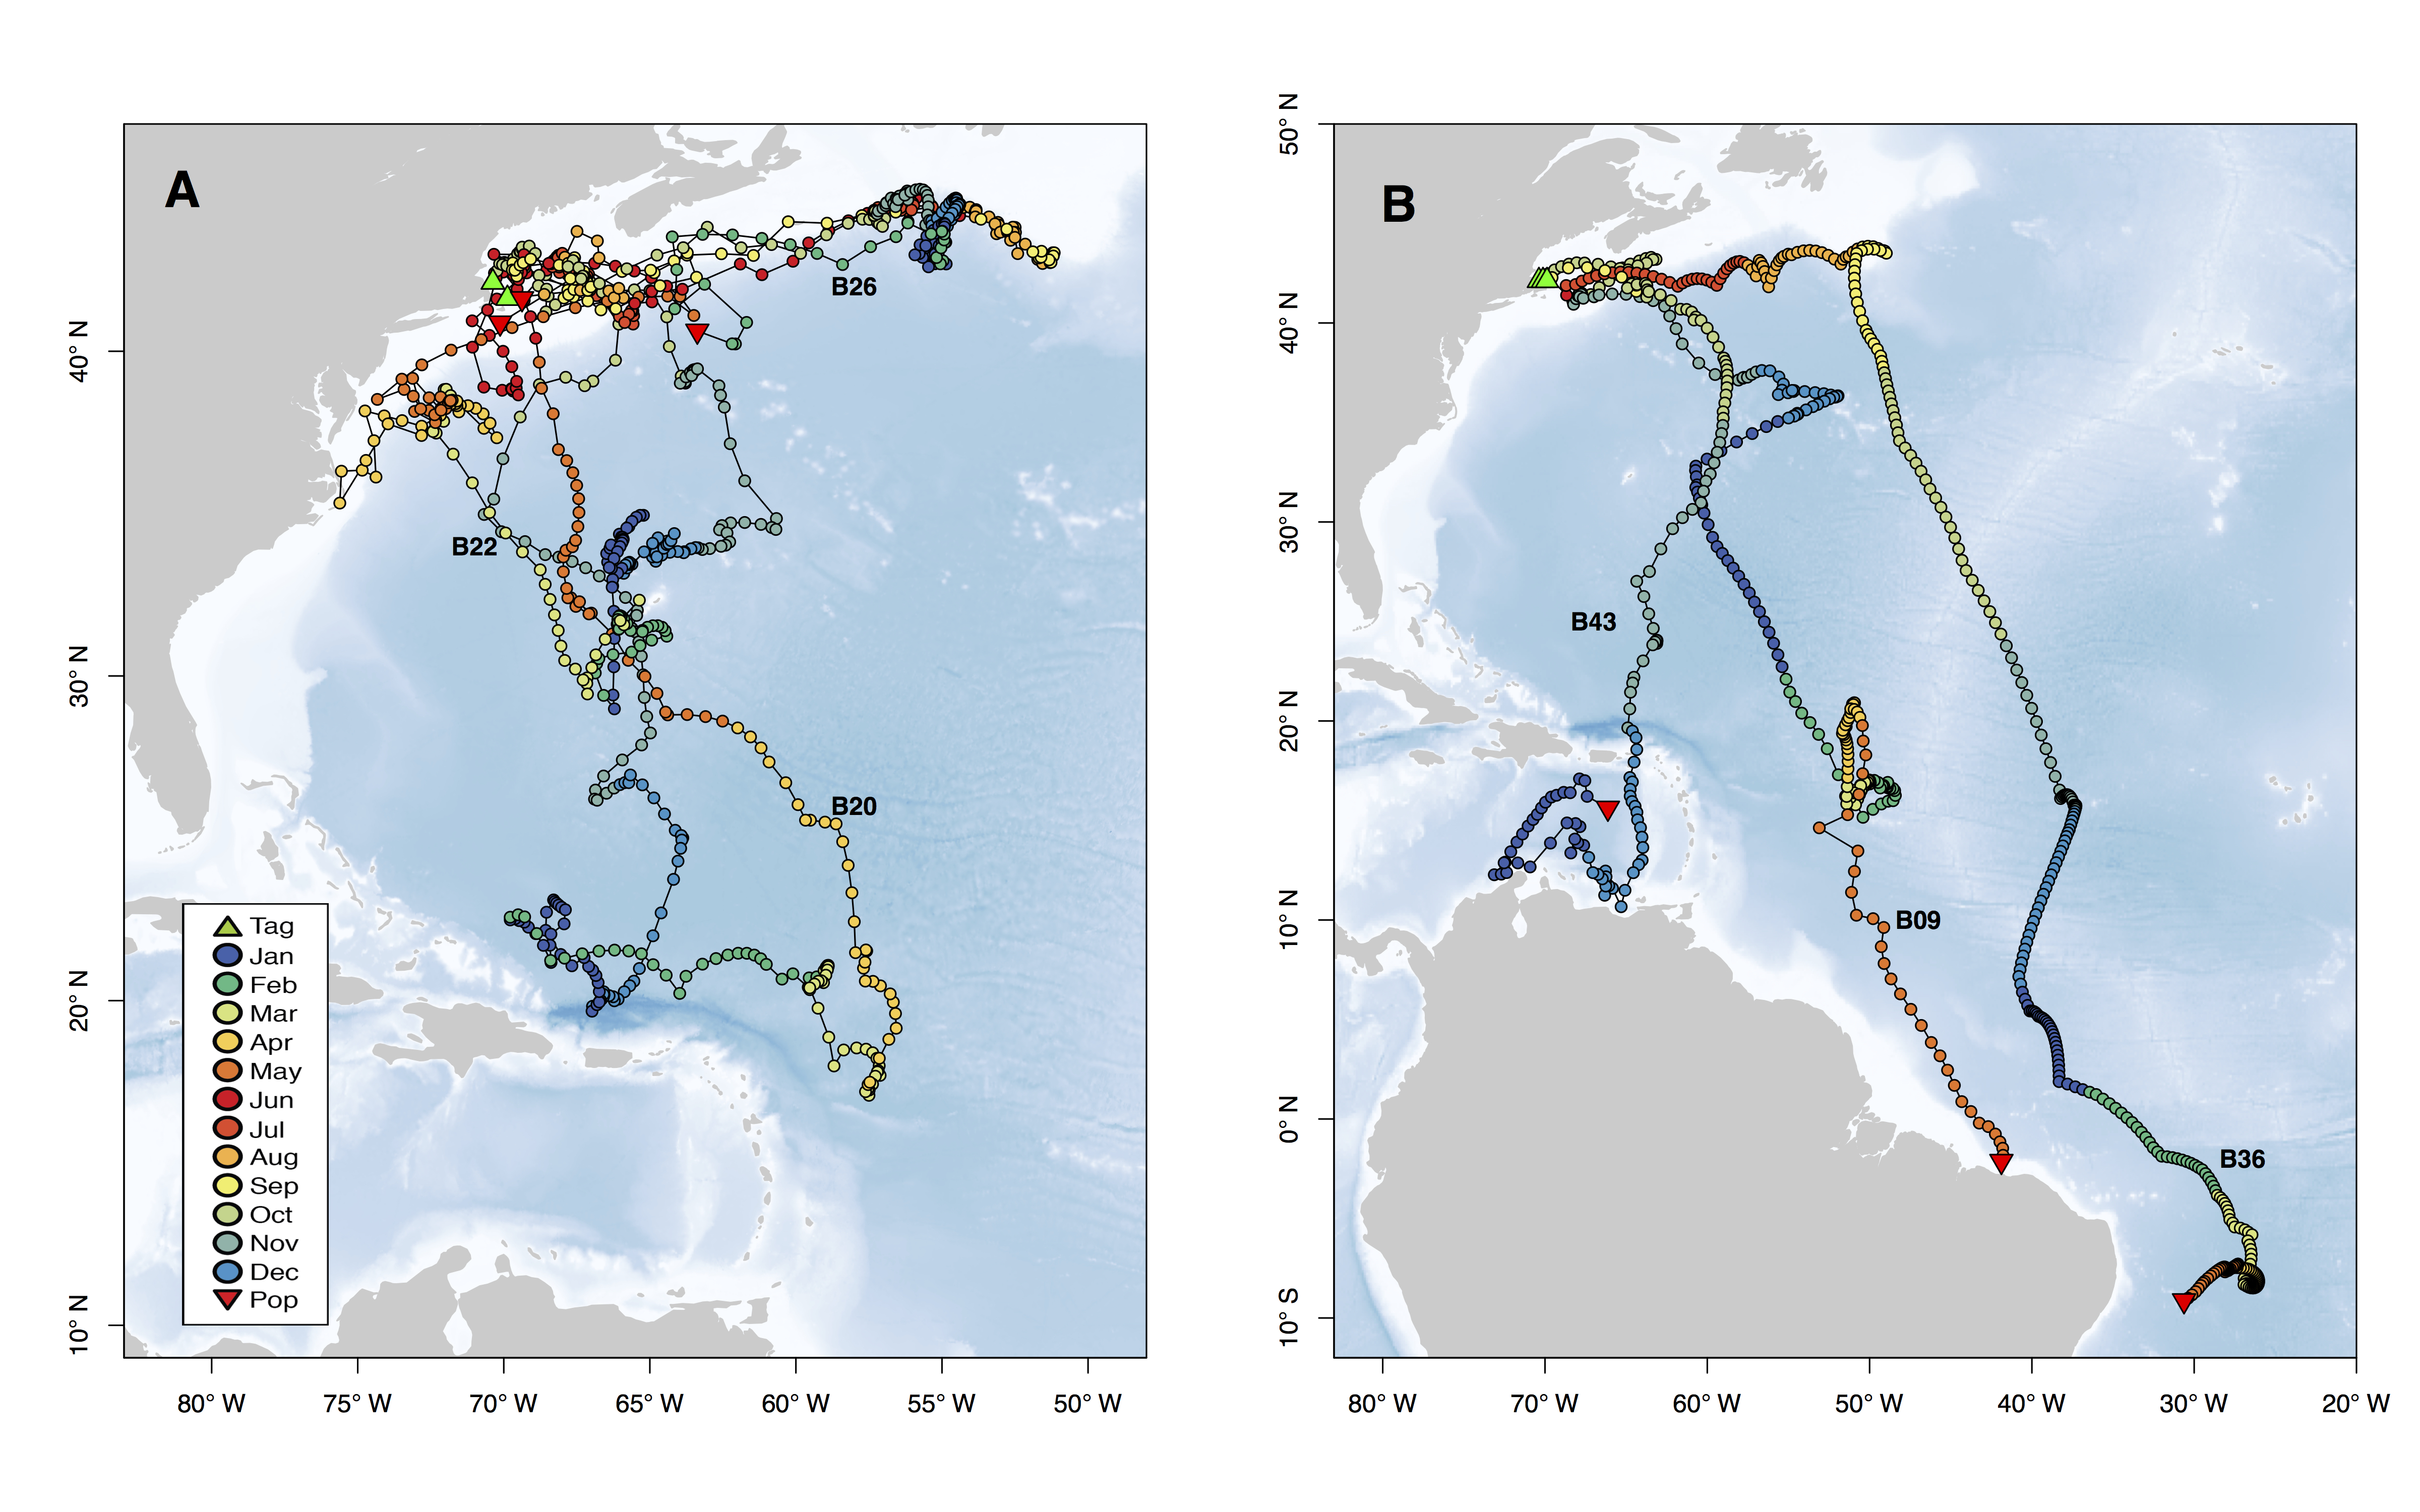
\includegraphics[width=1\textwidth]{images/C3_Fig5.jpg}
\caption[Representat]{Movements of selected individuals demonstrating representative behaviors exhibited by sharks in this study. Two selected individuals exhibited site fidelity to Cape Cod (B20, B22) and one individual overwintered near Newfoundland (B26, panel A). The variety of long distance movements are represented by three individuals with pop-up locations from the eastern Caribbean to the SE coast of Brazil (panel B). Tracks are plotted as points colored by month, and green and red triangles represent tag and pop-up locations, respectively. Text labels correspond to Shark ID in \cref{tab:c3t1}, and blue background indicates bathymetry of the region. Vertical habitat use of these selected individuals is shown in \cref{fig:c3f4} and \cref{fig:c3f6}. }
\label{fig:c3f5}
\end{figure}

%Figure 6:
\begin{figure}[t!]
\centering
\includegraphics[width=1\textwidth]{images/C3_Fig6.jpg}
\caption[Representative basking shark vertical data for long-range movements]{Daily depth-temperature profiles (row 1) and time-at-depth profiles (row 2) for 3 representative basking sharks (tracks plotted in Figure 5b). Note differing time scales (x-axis) among individuals.}
\label{fig:c3f6}
\end{figure}

%Figure 7:
\begin{figure}[t!]
\centering
\includegraphics[width=1\textwidth]{images/C3_Fig7.pdf}
\caption[short]{Vertical habitat envelopes of basking sharks. Temperature and depth data are binned every 1$^{\circ}$ and 25 m, respectively. Depths deeper than 1000 m are added to the last bin. The bounds for each region are shown as boxes in \cref{fig:c3f1}. Note the color bar is on a log scale. Summary statistics for each region and season are shown in \cref{tab:c3t2}, and blank panels indicate no data was collected for that region-season combination. }
\label{fig:c3f7}
\end{figure}

\section{Discussion}
It is increasingly clear that pelagic fishes throughout the global ocean conduct long-range migratory movements \citep[\emph{e.g. }][]{Block2011,Skomal2017a} and connect the surface and deep ocean through meso- and bathypelagic dive behavior \citep{Braun2014,Thorrold2014a}. The basking sharks tagged in the present study were no exception, making some of the longest horizontal movements of any ocean species tagged to date \citep{Block2005,Bonfil2005,Hays2006,Skomal2017a}.  Tagged individuals moved through several distinct water masses of the western Atlantic, and spent significant time in the mesopelagic, demonstrating the ability of basking sharks to traverse a wide range of environments from the surface to deep ocean across a 25$^{\circ}$C temperature range.

Movements through distinct water masses often coincided with varying periods of deep water occupation. Nearly all tagged individuals demonstrated a shift to residency from surface waters to deep in the meso- and bathypelagic during colder months that may explain the apparent disappearance of basking sharks during winter \citep{Parker1954}. While our results corroborate previous studies that suggest seasonally variable dive behavior \citep{Sims2003} and southward migration during winter \citep{Doherty2017}, sharks in this study made much more extensive movements throughout the open ocean than those observed in similar studies elsewhere \citep{Doherty2017} and spent up to several months at mesopelagic depths. Sharks tagged in the northeast Atlantic (NEA) did make dives to similar maximum depths ($\sim$50\% of tagged individuals dove below 1000 m; \citet{Doherty2017}) but averaged > 80\% of time above 200 m and < 10\% deeper than 500 m \citep{Sims2003, Doherty2017}. The mesopelagic occupation observed in this study suggests this behavior is much more ubiquitous among NWA basking sharks as they move throughout the open ocean than their NEA conspecifics that are relatively close to the coast and may be a product of the oceanography experienced (\emph{e.g.} warm, homogenous depth-temperature profiles in the Sargasso Sea) by these individuals in the open ocean of the NWA. 

The other main difference in behavior among these regions is the winter migration strategy. NEA basking sharks moved south from Ireland and the UK to the Bay of Biscay, but despite tagging 70 basking sharks with satellite tags, only 1 individual traversed > 20$^{\circ}$ of latitude after summer occupation of the far northern latitudes \citep{Doherty2017}. In contrast, winter movements at and beyond this scale were more commonly observed in the NWA \citep[][ and this study]{Skomal2009}. These movements refute the suggestion that basking sharks are largely restricted to temperate latitudes \citep{Sims1999,Sims2003,Gore2008,Doherty2017}, while NEA basking sharks did not traverse the equator, movements by individuals in the NWA demonstrate that tropical environments do not pose a barrier to basking shark movements.

It seems likely that the long-distance movements by basking sharks that we documented are driven, at least in part, by the dynamic oceanic environment of the western Atlantic Ocean. The NWA is punctuated by strong seasonal fluxes in pelagic primary productivity \citep{Miller2012} and temperature \citep{Talley2011}. The warm water and high productivity attract many species to the temperate NWA during summer \citealt[(e.g. basking sharks, ][]{Curtis2014}; \citealt[white sharks, ][]{Skomal2017a}). While it is clear basking sharks are able to tolerate sub-10$^{\circ}$C water for months at a time (B26 in \cref{fig:c3f4}; \citealt{Sims2008}), individuals in this study spent much of their time overwintering in warm, mesopelagic waters. In fact, as a whole, sharks spent more time in warmer water during deep occupation periods in winter as they moved south than they did during summer. While the function of this deep occupation is unknown, the Sargasso Sea is a relatively stable, warm water mass during winter months and may host prey opportunities for basking sharks in the mesopelagic, including a substantial deep scattering layer that overlaps with basking shark depth use (400-600 m; \citealt{Irigoien2014}) and potentially co-occurring anguillid eel spawning aggregations \citep{Wysujack2015}. These migrations away from the northern winter may also be associated with hotspots of relatively high production at lower latitudes \citep[(e.g. Brazilian shelf; ][]{Mourato2014}. Movements in this study demonstrated orientation to shelf edge habitats, particularly along the northern coast of Brazil during winter, that likely host persistent fronts \citep{LeFevre1987,Sims2008} and thus relatively high primary production even at low latitude. While basking sharks have been shown to orient to persistent seasonal fronts \citep{Miller2015}, most individual tracks in this study demonstrated intense occupation of near-shelf regions that was punctuated by lengthy offshore excursions. Thus, perhaps the combination of favorable growth energetics associated with warm overwintering habitat (relative to overwintering at temperate latitudes) and food availability drive southerly movements away from temperate latitudes for winter and the mesopelagic occupation in (sub)tropical waters observed here. However, further work is needed to test the role of energetics and food resources as drivers of basking shark migrations.

Movement patterns of tagged basking sharks may also be associated with reproduction \citep{Skomal2009}. Basking sharks are commonly observed along the northeastern US during summer, presumably to forage; however, mating may also occur during this period while sharks are aggregated and potential courtship behavior has been observed \citep{Wilson2004a}. Subsequent movements into the tropical Atlantic and occupation of mesopelagic depths may be a predator avoidance or parturition strategy as these environments are characterized by mild, stable conditions. This may further explain the lack of observations of pregnant females despite prolonged coastal fisheries in the NEA \citep{Sims2008}. Thus, while we did not observe significant differences in movement between sexes, the females that undertake long-range southerly migrations may be exploiting stable environmental conditions for gestation and parturition, and the stable habitat and relative lack of predators may provide suitable nursery habitat for neonates. The presence of < 2.5 m TL basking sharks in the Gulf of Mexico during spring \citep{Hoffmayer2011} lends some support for this hypothesis as it suggests that parturition is occurring during winter months in tropical or subtropical waters. The wide variation in movement patterns (> 50$^{\circ}$ range in latitude) suggests these migrations were not driven by a localized mating event somewhere in the Atlantic. Unfortunately, we were unable to sex a significant portion of tagged individuals in this study due to tag application methods, and the limited sample size of sexed individuals indicates no difference in movements between sexes that may further clarify reproductive hypotheses. 

Highly variable dive behavior, including extended forays away from the photic zone, exhibited by basking sharks made traditional light-based geolocation difficult in our study. Thus, we employed a recent advance \citep[(based on extensive work by ][]{Pedersen2008, Pedersen2011a} in geolocation analysis methods to supplement missing light data with other forms of data recorded on the tag \citep{Braun2018a}. Depth-temperature profiles, in particular, provided substantially more information to be used for geolocation than light and SST data used in traditional geolocation approaches. These profiles provided observations that were used for geolocation when tagged individuals were away from the surface and the tags couldn’t collect light and SST metrics. In addition, the profile data yielded diagnostic depth-temperature profiles that can be compared to modeled or in situ oceanographic data for reducing geolocation error \citep{Braun2018a}. By using the high-resolution (0.08$^{\circ}$) HYCOM reanalysis product, we were able to leverage the synoptic daily coverage of an oceanographic model that incorporates available in situ data to improve geolocation estimates. While previous tracking studies have shown some problems with the HYCOM reanalysis product being used to construct tracks through the Gulf Stream eddy field \citep{Braun2018a}, the majority of basking sharks in this study moved latitudinally and spent relatively little time in the most dynamic regions of the NWA. 

Model outputs also indicated a higher likelihood of "resident-like" movements in productive shelf habitats around New England and off the Antilles and South America. It is likely these restricted movements are indicative of foraging in these relatively productive shelf habitats \citep{Mourato2014}. In contrast, migratory movements (4 $m s^{-1}$) were more likely in pelagic waters, including during overwintering in the Sargasso Sea. Because of model formulation, the higher speeds that we classified as "migratory" may also be more likely, overall, due to the scale at which the observation likelihoods are formulated. For instance, if tag-based SST corresponds to remotely sensed SST over a broad area (\emph{e.g.} Sargasso Sea), we may expect migratory behavior to be more likely than the resident behavior that would result from more constrained likelihoods (\emph{e.g.} tag-based SST matching more closely to a confined region). While this approach is significantly more computationally-intensive than traditional light-based geolocation approaches, comparing tag data directly to in situ and/or modeled oceanographic profiles from the same time frame results in a more realistic representation of shark movements and the oceanographic environment they inhabit.

The basking shark tracks documented here represent the largest scale movements reported for basking sharks, including one individual’s estimated track distance covering >17,000 km, and the deepest dive recorded by a basking shark (1504 m). The observed tracks further expand the known range of basking sharks reported by \citep*{Skomal2009}. We recorded 3 individuals making transequatorial migrations yet no tagged individuals made significant longitudinal movements toward the NEA. North-south movements were, therefore, much more common in the portion of the NWA population sampled here than east-west movements that may, in turn, limit the exchange of genetic material between the NWA and NEA. In contrast, \citep*{Gore2008} found that one of two satellite-tagged basking sharks moved from the Isle of Man to the eastern coast of Newfoundland in less than 3 months. In addition, there is little evidence for genetic structuring of basking sharks in the Atlantic \citep*{Hoelzel2006}, suggesting sufficient connectivity to at least maintain panmixia between NEA and NWA populations.

\section{Conclusion}
The current reliance on light levels for geolocation of many marine fishes renders geolocation impossible when tagged individuals spend significant time below the euphotic zone. Tagged sharks in this study spent significant time at mesopelagic depths, particularly during winter, at which light levels were too low for geolocation. We supplemented light-based geolocation with position estimates generated by matching depth-temperature profiles collected by the sharks’ tags to in situ or modeled oceanographic profiles. Our approach provided considerably more information on movement patterns than are typically available from PSAT data with limited light-level information, providing a valuable method for studying marine species that do not frequent the euphotic zone. The resulting basking shark tracks demonstrated large-scale movements up to over 17,000 km from Cape Cod to southern Brazil, winter residency in New England waters, and a range of behaviors in between. Most individuals exhibited seasonal movements into the Sargasso Sea during winter and multiple deployments of sufficient duration captured the return migration to Cape Cod the subsequent summer. Basking sharks in this study traversed multiple distinct water masses through the western Atlantic and exhibited basin-scale movements that warrant international cooperation for adequate management of this species. Winter habitat use was characterized by occupation of mesopelagic waters at low latitudes during which individuals often left the surface for months at a time. This cryptic deep-water overwintering provides impetus for further study of this poorly understood species.

% table 1: tag metadata and results
\begin{table}
\caption{Summary information from satellite tag deployments on Cetorhinus maximus in the NW Atlantic. Identification number of each individual is shown along with the tag model. All tags were manufactured by Wildlife Computers, Inc. (Redmond, WA, USA). Est. Length = the total length (m) of the individual tagged as estimated from the tagging vessel; Sex = male (M) or female (F) where determination was possible by visual observation of presence or absence of claspers between the pelvic fins, no entry indicates that sex could not be confidently determined; Pop Lat / Long = coordinates of tag detachment location; Deploy Duration = number of days between tag deployment and detachment; Max Depth = the deepest depth (m) reported by the tag during the deployment; Track Distance = cumulative distance of most probable track; Light, SST and depth-temperature profile (PDT) columns indicate percent of deployment days with light-based location estimates, sea surface temperature data and depth-temperature profiles. Observation likelihoods are those observations used in HMMoce to construct the most probable track for each tagged animal: L=light-based longitude, S=sea surface temperature, H=HYCOM depth-temperature profiles, W=World Ocean Atlas depth-temperature profiles, O=integrated Ocean Heat Content, F=Fastloc GPS, DD=data deficient.}
\label{tab:c3t1}
\centering
\begin{tabular}[t]{lrllrlll}
\toprule
Shark ID & Tag Type & Tag Date & Est. Length (m) & Sex & Pop Lat (\deg N) & Pop Long (\deg W) & Deploy Duration (d) & Max Depth (m) & Track Distance (km) & Light (\%) & SST (\%) & PDT (\%) & Observation Likelihoods \\
\midrule


\bottomrule
\end{tabular}
\end{table}

% table 2: vertical summary statistics
\begin{table}
\caption[Vertical habitat envelope summary statistics]{Summary statistics for vertical habitat envelopes in \cref{fig:c3f7} by region and season. Reported values are formatted as median(minimum-maximum) for sea surface temperature (SST), minimum daily depth (Min Z), maximum daily depth (Max Z) and minimum daily temperature (Min T). Temperatures are $^{\circ}$C and depths are in meters. Sample sizes (N) indicate total number of data points (not individual profiles) and are shown for each region-season combination. Blank combinations in the table indicate no data was collected for that combination. Note these data were restricted to the spatial areas of interest as shown in Figure 1 and may not exactly match reported statistics in the text which included all data.}
\label{tab:c3t2}
\centering
\begin{tabular}[t]{lrllrlll}
\toprule
 &  & New England & Sargasso Sea & Antillean Arc & South America \\
\midrule


\bottomrule
\end{tabular}
\end{table}


\chapter{Functional group-specific traits drive phytoplankton dynamics in the oligotrophic ocean}

\raggedbottom

%\begin{singlespace}
%Harriet Alexander$^{1,2}$, M\'{o}nica Rouco$^3$, Sheean T. Haley$^3$, Samuel T. Wilson$^4$, David M. Karl$^4$, Sonya T. Dyhrman$^{3}$\\
%\\
%$^{1}$ MIT-WHOI Joint Program in Oceanography/Applied Ocean Science and Engineering, Cambridge, MA 02139, USA\\
%$^2$ Biology Department, Woods Hole Oceanographic Institution, Woods Hole, MA 02543, USA\\
%$^3$ Department of Earth and Environmental Sciences Lamont-Doherty Earth Observatory, Columbia University, Palisades, NY 10964\\
%$^4$ Daniel K. Inouye Center for Microbial Oceanography: Research and Education, Department of Oceanography, University of Hawaii, Honolulu, HI 96822, USA\\
%\\
{\let\thefootnote\relax\footnotetext{This chapter was originally published as Alexander, H., R\'{o}uco, M., Haley, S.T., Wilson, S.T., Karl, D.M., and Dyhrman, S.T. (2015). \href{http://www.pnas.org/content/112/44/E5972.full}{Functional group-specific traits drive phytoplankton dynamics in the oligotrophic ocean.} \emph{Proc. Natl. Acad. Sci. U. S. A.} 112:44, E5972-E5979.}}
{\let\thefootnote\relax\footnotetext{H.A. and S.T.D. designed research; H.A., M.R., S.T.H., S.T.W., and S.T.D. performed research; H.A., D.M.K., and S.T.D. analyzed data; H.A. and S.T.D. wrote the paper; and M.R., S.T.H., S.T.W., and D.M.K. contributed to the writing of the paper.}}



%\end{singlespace}
\clearpage

\section{Abstract} 
A diverse microbial assemblage in the ocean is responsible for nearly half of global primary production. It has been hypothesized and experimentally demonstrated that nutrient loading can stimulate blooms of large eukaryotic phytoplankton in oligotrophic systems. Although central to better balancing biogeochemical models, knowledge of the metabolic traits that govern the dynamics of these bloom-forming phytoplankton is limited. We employed eukaryotic metatranscriptomic techniques to identify the metabolic basis of functional group-specific traits that may drive the shift between net heterotrophy and autotrophy in the oligotrophic ocean. Replicated blooms were simulated by deep seawater addition to mimic nutrient loading in the North Pacific Subtropical Gyre and the transcriptional responses of phytoplankton functional groups were assayed. Responses of the diatom, haptophyte, and dinoflagellate functional groups in simulated blooms were unique, with diatoms and haptophytes significantly (95\% confidence) shifting their quantitative metabolic fingerprint from the \textit{in situ} condition, while dinoflagellates showed little response. Significantly differentially abundant genes identified the importance of co-limitation by nutrients, metals, and vitamins in eukaryotic phytoplankton metabolism and bloom formation in this system. The variable transcript allocation ratio, used to quantify transcript reallocation following DSW amendment, differed for diatoms and haptophytes, reflecting the long-standing paradigm of phytoplankton r- and K-type growth strategies. While the underlying metabolic potential of the large eukaryotic phytoplankton was consistently present, the lack of a bloom during the study period suggests a crucial dependence on physical and biogeochemical forcing, which are susceptible to alteration with changing climate. 
 
\section{Introduction}
It has been postulated that the net oxygen state of oligotrophic systems is controlled by irregular blooms of large eukaryotic phytoplankton \citep{Karl2003}, which have been shown to respond to nutrient input in open ocean ecosystems \citep{McAndrew2007}. Nutrient loading shifts the community away from a tightly regenerating microbial loop, based on small phytoplankton (typically bacterioplankton), towards a community with a higher proportion of larger phytoplankton cells (typically eukaryotic phytoplankton) and, consequently, more carbon export \citep{McAndrew2007}. Data from Station ALOHA in the oligotrophic North Pacific Subtropical Gyre (NPSG) during the summer period have identified increased export of organic carbon, diatomassociated biogenic silica (BSi), and, to a lesser extent, particulate inorganic carbon (PIC) associated with calcification \citep{Karl2012}. These increases are potentially a result of nutrient-driven community shifts. Blooms of eukaryotic phytoplankton in oligotrophic environments are often dominated by the diatom functional group \citep{Villareal2012} and may determine the balance between net heterotrophic and net autotrophic conditions \citep{Karl2003}. Such blooms, however, are thought to be under-sampled and may often go undetected in satellite ocean color records \citep{Villareal2011}. Consequently, the drivers of bloom formation and concomitant carbon export remain poorly understood, particularly in critical oligotrophic systems. \par 
Though central to better balancing global biogeochemical models of GPP \citep{Lopez-Urrutia2006}, knowledge of the biogeochemical drivers that govern the dynamics of these bloom-forming organisms in oligotrophic systems is limited. Nutrient environments are integral to the structuring of phytoplankton communities \citep{Margalef1978, Tilman1977, Cavender-Bares2001} and initiating blooms. Originally thought to be a stable low-fluctuating habitat, long-term monitoring at Station ALOHA has demonstrated that within the constraints of an oligotrophic ecosystem the nutrient regime can be quite dynamic, alternating in controlling factors over many time scales \citep{Karl2001}. These oscillations may be driven by biological (e.g. bloom of N2-fixing cyanobacteria, which draw down P or Fe, while injecting new nitrogen into the system \citep{Karl2002}), physical (e.g. nutrient supply from transient eddies \citep{Benitez-Nelson2007}), or anthropogenic (e.g. atmospheric deposition of nutrients \citep{Kim2014}) forcing.  Regardless of the source, these nutrient-loading events could act to stimulate blooms in the large eukaryotic phytoplankton community.  Historically, the distributions of key eukaryotic phytoplankton function groups have been tracked relative to nutrient stoichiometries to examine how nutrients influence the physiological ecology of different functional groups like diatoms and haptophytes \citep{Cortes2001, Villareal2012}. Although valuable, it is still difficult to relate stoichiometries to the dynamics of bloom formation and, in particular, to patterns in key groups like diatoms without specific measures of functional group physiology. \par
Molecular-level tools that can track transcripts, proteins, or even metabolites and biochemicals in a taxon-specific way are increasingly being employed in cultures and field populations to track metabolic capacity and physiological responses \citep{Marchetti2012a, Alexander2015, Dupont2015, Pearson2015, Ottesen2014, Hennon2015, Dyhrman2012, Amin2015}. Molecular assessment of physiology for eukaryotic populations is most tractable in coastal systems with high biomass \citep{Alexander2015, Dupont2015}, so, in oligotrophic ocean regions, molecular studies of physiology have typically been limited to the numerically abundant members of the microbial community: picoplankton (cyanobacteria, heterotrophic bacteria, and small picoeukaryotes). Groundbreaking studies have demonstrated the responsiveness of the dominant picoplankton community to pulses of deep seawater (DSW) \citep{Shi2012} and of DOM \citep{McCarren2010}, as well as the diel synchrony of the photosynthetic and heterotrophic communities \citep{Ottesen2014}, yet were limited in their coverage of the rare, large eukaryotic fraction due both to the low biomass of their standing stock and the lack of reference sequences. A recent world ocean survey has highlighted the diversity encompassed within the eukaryotic planktonic community \citep{DeVargas2015} and suggested that the structuring of these communities may be driven by physical and chemical oceanographic features \citep{Villar2015}. Yet again, the responsiveness of these keystone eukaryotic phytoplankton communities to changing environmental conditions remains poorly described and understood. 
New resources, including a new marine microbial eukaryote sequencing initiative \citep{Keeling2014}, in combination with the bioinformatic pipeline used here are making possible the study of oligotrophic eukaryotic phytoplankton with unprecedented mechanistic resolution. Here we examined potential biogeochemical controls on phytoplankton bloom formation in the NPSG and the metabolic traits that govern the distribution and responses of unique functional groups. \par

\section{Materials and Methods}
\subsection{Sample collection}
Seawater for the \textit{in situ} eukaryote community mRNA analysis was collected at the HOT, Station ALOHA ($22^\circ 45^\prime$ N, $158^\circ 00^\prime$ W) from a depth of 25 $m$ at 1400 hrs (local time) on three occasions during August and September 2012 as part of the HOE-DYLAN research expedition aboard the R/V Kilo Moana. Hydrocasts for sampling were performed using a conductivity-temperature-depth (CTD) rosette water sampler equipped with 24 Scripps 12-L sampling bottles. Water was collected in acid-washed 20-L carboys and approximately 60-L of seawater was prescreened through $200 \mu m$ mesh and then filtered onto polycarbonate filters ($5.0 \mu m$ pore size, $47 mm$, Whatman) by way of peristaltic pump. This size fraction was targeted to sample large eukaryotic phytoplankton, which are known to form blooms and contribute to export flux in the NPSG. Filters were changed every 20 minutes or when flow rate decreased. Filters were placed in cryovials and stored in liquid nitrogen until mRNA extraction. The total length of filtration time did not exceed 3 hours. Nutrient delivery in the ocean is highly variable; here we chose to model a single nutrient pulse. The incubation experiments were performed with two treatments: a DSW treatment, which included 10\% 0.2 $\mu m$ filtered seawater collected from 700 $m$ added to whole seawater collected at 25 m and a control treatment with no addition (Table \ref{tab:a4t1}). Triplicate 20-L carboys of each treatment were incubated at 30\% surface light levels using on-deck incubators for 7 days and processed as described above on the final day at 1400 h (local time). Nutrient concentrations for phosphate (PO$_4$), nitrate and nitrite [NO$_2$+NO$_3$], and silicate [SiO$_4$] (Table \ref{tab:a4t1}) were measured by filtering 125 $mL$ of seawater through a 0.2 $\mu m$, 47-$mm$ polycarbonate filter, and stored frozen ($−20^\circ$C) in acid washed bottles until analysis at the Chesapeake Bay Lab at the University of Maryland according to the facility’s protocols. Chlorophyll a was measured on whole water samples collected onto GF\/F filters ($25 mm$, Whatman) using a 90\% acetone extraction and assayed by fluorescence using the AquaFluor Turner TD700 \citep{Parsons1984}. There was little difference between the \textit{in situ} sample and the control treatment both with regards to total chlorophyll a concentration and transcriptional profile (Figure \ref{fig:a4f1}, Figure \ref{fig:a4f7}).  There was no significance difference in QMF between the control treatment at the final time point and the \textit{in situ} sample taken at the start of the incubation (Figure \ref{fig:a4f7}). To most conservatively compare non-bloom and bloom scenarios, analyses thus focused on the comparison of the \textit{in situ} community to the DSW amended samples. \par

\subsection{RNA extraction and sequencing}
RNA was extracted from individual filters with the RNeasy Mini Kit (Qiagen), following a modified version of the yeast protocol. Briefly, lysis buffer and RNA-clean zirconia/silica beads was added to the filter and samples were vortexed for 1 minute, placed on ice for 30 seconds, and then vortexed again for 1 minute. Samples were then processed following the yeast protocol. The resulting RNA was eluted in water and then treated for possible DNA contamination using TURBO DNA-free Kit (Ambion) following the Rigorous DNase protocol. RNA from individual filters was then pooled by sample, using the RNA Cleanup Protocol from the RNeasy Mini Kit (Qiagen). The resulting RNA sample thus represented approximately 60 L of total seawater for the \textit{in situ} sample. Filters were pooled across like triplicate bottles by treatment, totaling 60 L from each of the incubation treatments. The total RNA sample was then enriched for eukaryotic mRNA through a poly-A pull down. The resulting enriched mRNA sample then went through library preparation with the Illumina TruSeq mRNA Prep Kit (Illumina). Libraries were sequenced with the Illumina HiSeq2000 at Columbia Genome Center (New York, NY). Each sample was sequenced to produce a targeted 60 million, 100 base pair, paired end reads. These environmental sequence data are deposited in the Sequence Read Archive (SRA) through the National Center for Biotechnology Information (NCBI) under accession number \href{http://google.com}{SRP056385}. Raw sequence data quality was visualized using FastQC and then cleaned and trimmed using Trimmomatic v 0.27 (paired end mode; 6-base pair wide sliding window for quality below 20; minimum length 25 base pair). \par
\subsection{Genome database creation and mapping}
Environmentally relevant algal genomes (\textit{Aureococcus anophagefferens} CCMP1984 v1.0, \textit{Emiliania huxleyi} CCMP1516 v1.0, \textit{Fragilariopsis cylindrus} CCMP1102 v1.0, \textit{Micromonas pusilla} RCC 299 v3.0, \textit{Ostreococcus lucimarinus} v2.0, \textit{Ostreococcus tauri} v2.0, \textit{Phaeodactylum tricornutum} CCMP632 v2.0, \textit{Pseudo-nitzschia multiseries} CLN-47 v1.0, \textit{Thalassiosira pseudonana} CCMP1335 v3.0) were collected from the Joint Genome Institute \href{http://genome.jgi.doe.gov/}{(JGI) database} and concatenated. Trimmed, paired-end reads from each of the samples were mapped to this concatenated genome library using the Burrows-Wheeler Aligner \citep{Li2010} (BWA-mem, parameters: -k 10 -aM) and then counted using the HTSeq 0.6.1 package \citep{Anders2014}.\par 
\subsection{MMETSP database creation and mapping}
Transcriptome sequences and annotations generated through the Marine Microbial Eukaryote Transcriptome Sequencing Project (MMETSP) that were made public as of 17 March 2014 were collected, representing 401 transcriptomes across 209 species or cultured isolates. Transcriptomes from like species (regardless of strain or condition) and cultured isolates were pooled and clustered using CD-HIT-EST (98\% identity; word size of 9). The resulting clustered set of transcripts was considered to be the representative transcriptome for the species or cultured isolate. Transcriptomes were annotated with KEGG Orthology annotations using the bi-directional best hit (BBH) method through the KEGG Automatic Annotation Server (KAAS) \citep{Moriya2007}. It is worth noting that the KEGG module names are human defined and some genes are artificially grouped in the context of phytoplankton metabolism.  For example, this is the case with the ``methane metabolism'' module, which includes a suite of genes related to carbon not specifically methane metabolism. The 209 transcriptomes created in this manner were concatenated to form a comprehensive species-level transcriptome database from the MMETSP library. Due to the large size of the resulting MMETSP database, trimmed reads were mapped to the MMETSP using the Burrows-Wheeler Aligner \citep{Li2010} (BWA-mem, parameters: -k 10 -aM) and then counted using the HTSeq 0.6.1 package \citep{Anders2014}. \par
\subsection{Differential expression analysis}
Counts obtained from HTSeq were pooled for like-KEGG orthologs across all species in a functional group. The quantitative metabolic fingerprint (QMF) was assessed by normalizing global patterns of expression at the module-level to the total mapped reads, an approach similar to those used in several metagenomic and metatranscriptomic studies focused on prokaryotes \citep{Shi2011, Ottesen2014, Shi2012}. PCA and confidence ellipses of the QMF signals by functional group and sample type (\textit{in situ}, no addition control, and DSW addition) were calculated and visualized using FactorMineR package in R (Figure \ref{fig:c4f2}, Figure \ref{fig:a4f7}). No significant difference was seen between the \textit{in situ} and no addition control samples (Figure \ref{fig:a4f7}). For each functional group, the pooled KEGG counts from the \textit{in situ} samples (S1-S3) were compared to those from the corresponding DSW amendment (E1-E3) using Analysis of Sequence Counts (ASC), an empirical Bayes method \citep{Wu2010}. Genes were considered to be differentially abundant between treatments if for a fold change of 2.0 the posterior probability (post-$p$) was greater than 0.95 \citep{Dyhrman2012}. Patterns of differential abundance were visualized using Circos \citep{Krzywinski2009}. Global shifts in the expression of genes independent of functional group were assessed with TMM normalization using the Microbial Assemblage Normalized Transcript Analysis package (MANTA, v. 1.12.0)\citep{Marchetti2012a}. \par
\subsection{Variable transcript allocation modeling} 
Variable transcript allocation following DSW amendment was calculated for each functional group. Though there was a normal distribution of log fold change across all functional groups, the means were off-set for the diatoms and the haptophytes (Figure \ref{fig:a4f4}). From the set of all genes ($G$), the genes which had statistically significant increased transcript abundance (Equation \ref{eq:c4e1}) and decreased transcript abundance (Equation \ref{eq:c4e2}) as identified with ASC (2 fold change, post-$p > 0.95$) \citep{Wu2010} in DSW amended treatments (E) relative to the \textit{in situ} sample (S) were considered. 
%Equation 1 and 2
\begin{equation}
	\label{eq:c4e1}
	 U = \{g : post-p(\frac{T_{E,g}}{T_{S,g}} > 2) > 0.95, g \epsilon G\}
\end{equation}

\begin{equation}
	\label{eq:c4e2}
	 D = \{g : post-p(\frac{T_{S,g}}{T_{E,g}} > 2) > 0.95, g \epsilon G\}
\end{equation}
A variable transcript allocation score ($VTA$) was calculated for both the set of genes with both increased (Equation \ref{eq:c4e3}) and decreased (Equation \ref{eq:c4e4}) abundance, taking the ratio of the summed transcripts per million (T) for the \textit{in situ} (S) and experimental DSW amended treatments (E) of every gene ($u$ or $d$) within the set of significantly differentially abundant genes (U or D). $VTA$ scores were calculated so as to always be greater than one, thus the $VTA_{Dn}$ sums the reciprocal of the ratio summed in $VTA_{Up}$ (Equations \ref{eq:c4e3} and \ref{eq:c4e4}). $VTA_{Dn}$ is the magnitude of the decreased transcriptional response following DSW addition, while the $VTA_{Up}$ is the magnitude of the increased transcriptional response following DSW addition. $VTA_{Up}$ and $VTA_{Dn}$, as ratios, focus on the total transcript pool shifted between S and E rather than the number of genes with differential abundance. As such, we can directly compare these two ratios with $VTAR$ (Equation \ref{eq:c4e5}) and assess the metabolic trait of reallocation efficiency. If $VTAR > 1$, there was a larger transcript pool (TPM) in genes that were increased than were decreased, indicating an efficient reallocation of the transcript pool. By contrast, if $VTAR < 1$, less TPM was increased than was decreased. This model defines the total metabolic responsiveness as a trait that can be compared between the functional groups. 
%Equations 3, 4, and 5
\begin{equation}
	\label{eq:c4e3}
	VTA_{Up} = \sum_{u\epsilon U} \frac{T_{E,u}}{T_{S,u}}
\end{equation}
\begin{equation}
	\label{eq:c4e4}
	VTA_{Dn} = \sum_{d\epsilon D} \frac{T_{S,d}}{T_{E,d}}
\end{equation}
\begin{equation}
	\label{eq:c4e5}
	VTAR = \frac{VTA_{Up}}{VTA_{Dn}}
\end{equation}

\section{Results and Discussion}
We leveraged increases in reference sequence availability \citep{Keeling2014} to identify the expressed metabolic capabilities of different phytoplankton functional groups. Total RNA from the eukaryotic community ($>5 \mu m$) of the surface mixed layer at Station ALOHA was sequenced (60 million 100 base pair, poly-A selected, paired end reads) from three samples collected during August-September 2012 (S1-S3). To better understand the underlying functional group-specific metabolism associated with blooms, three blooms were simulated via on-deck incubations. While there are many potential nutrient inputs or bloom drivers (e.g. biologically fixed nitrogen), these blooms were simulated through the addition of deep seawater (DSW) to mimic nutrient loading by upwelling.  These incubation experiments were modeled after \citet{McAndrew2007} and were performed in conjunction with each of the in situ samples, amending surface water with a 10\% mixture by volume of water from below the nutricline (700 m). Sequence reads from the in situ samples (S1-S3) and the bloom simulations (E1-E3) were mapped to 1) non-symbiotic microalgal genomes and 2) a custom database comprised of all publically available transcriptomes as of 17 March 2014 from the Marine Microbial Eukaryotic Transcriptome Project (MMETSP) \citep{Keeling2014}.\par 
The MMETSP provides a 50x expansion of molecular data across the eukaryotic tree of life, which both better reflects the broad diversity within the protists and adds higher-definition coverage for well-studied groups such as diatoms and dinoflagellates \citep{Keeling2014}. Our leveraging of this database for the pipeline developed herein enabled unprecedented identification of taxonomic composition (58-62\% of reads identified) compared to mapping the same dataset to genomes (12-14\%), which have been used in previous studies \citep{Marchetti2012a}. Due to the taxonomic bias of the non-symbiotic algal genomes, the majority of reads from the in situ eukaryote community mRNA samples were annotated as diatoms or haptophytes. When mapped to the custom MMETSP database, however, dinoflagellates dominated, constituting 36-40\% of the mapped reads, with the diatoms and haptophytes the next most highly represented functional groups (Figure \ref{fig:c4f1}A). The dominance of dinoflagellates in the 5 μm size fraction, confirmed in historic surface pigment analyses at Station ALOHA \citep{Letelier1993}, stands in contrast to previous eukaryotic metatranscriptome studies in the oligotrophic ocean where they accounted for < 5\% of reads \citep{Marchetti2012a}. Although clearly present and important to the community, dinoflagellate read abundance here and in sediment trap data collected during the same cruise series \citep{Fontanez2015} may be magnified by their large transcript pool \citep{Moustafa2010, Hackett2004}. \par

% Figure 1: taxonomic distribution of reads
\begin{figure}[p!]
  \centering
    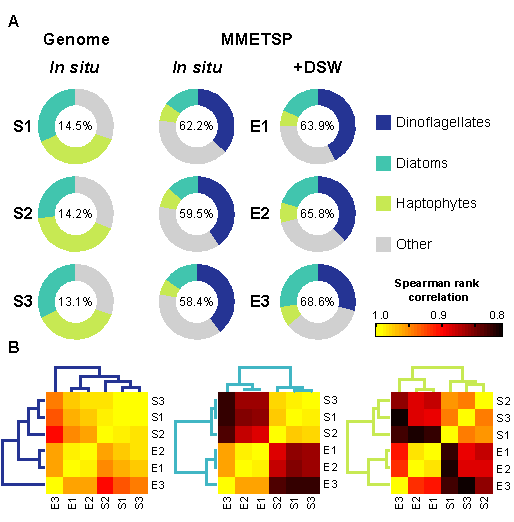
\includegraphics[width=.8\textwidth]{Images/C4_Figure1_Final.png}
    \caption[Taxonomic distribution in mRNA mapped reads consistent across time but altered by deep seawater (DSW) addition]{Taxonomic distribution in mRNA mapped reads consistent across time but altered by deep seawater (DSW) addition. Sequences collected during the summer of 2012 at Station ALOHA (S1: 6 August, S2: 24 August, S3: 2 September) and corresponding deep seawater (DSW) incubation experiments (E1-E3) were mapped to two custom databases: 1) non-symbiotic microalgal genomes and 2) all freely available transcriptomes from the MMETSP as of 17 March 2014. (A) Taxonomic affiliation of reads across the three most abundant functional groups: dinoflagellates, diatoms, and haptophytes mapped to both the genome and MMETSP databases for S1-S3. The corresponding DSW addition incubations E1-E3 were only mapped the MMETSP database. The percent of total reads mapped is indicated inside each of the circles. (B) Spearman rank correlation for species composition shifts within each of the three functional groups across S1-S3 and E1-E3.}
  \label{fig:c4f1}
\end{figure}

The species composition of the functional groups, reflected in rank abundance (Figure \ref{fig:c4f1}B), was highly conserved across all three in situ samples (S1-S3), underscoring the stability of phytoplankton populations in this well-studied oligotrophic system. Between 18.1 and 20.7\% of reads mapped to the MMETSP database were annotated with KEGG orthology, elucidating differences in the mRNA distribution between functional groups at the pathway level. Looking at the module-level, the general distribution of transcripts in proportion to the total was assessed using quantitative metabolic fingerprinting (QMF) \citep{Alexander2015}. Diatoms have a larger proportion of mRNA in the transport-related system (e.g. metallic cation, B12, phosphate, and amino acid) compared to haptophytes and dinoflagellates (Figure \ref{fig:c4f2}A). Purine metabolism was consistently a large component of haptophyte QMF (5.6-27\%), an order of magnitude higher than diatoms and dinoflagellates (1-2\%). Purine nucleotides may represent a source of DON accessible to haptophytes, as haptophytes have been found to grow on purines as their sole N source \citep{Palenik1997}. As the precursors for nucleic acid biosynthesis, purine uptake in the ocean has also been attributed to nucleotide salvage \citep{Winn1984}. These functional group differences observed at the module-level are underscored by principle component analysis (PCA) with the QMF for each functional group differing with 95\% confidence (Figure \ref{fig:c4f2}B) and are suggestive of metabolic partitioning between functional groups. Within a functional group, the QMF was stable across time (Figure \ref{fig:c4f2}A), in contrast to the variability observed in coastal systems over similar time scales \citep{Alexander2015, Dupont2015}. This stability likely reflects both the unique physiological attributes of oligotrophic phytoplankton as well as the comparatively static geochemical environment. \par
%Figure 2. QMF and Circos

\begin{figure}[p!]
  \centerline{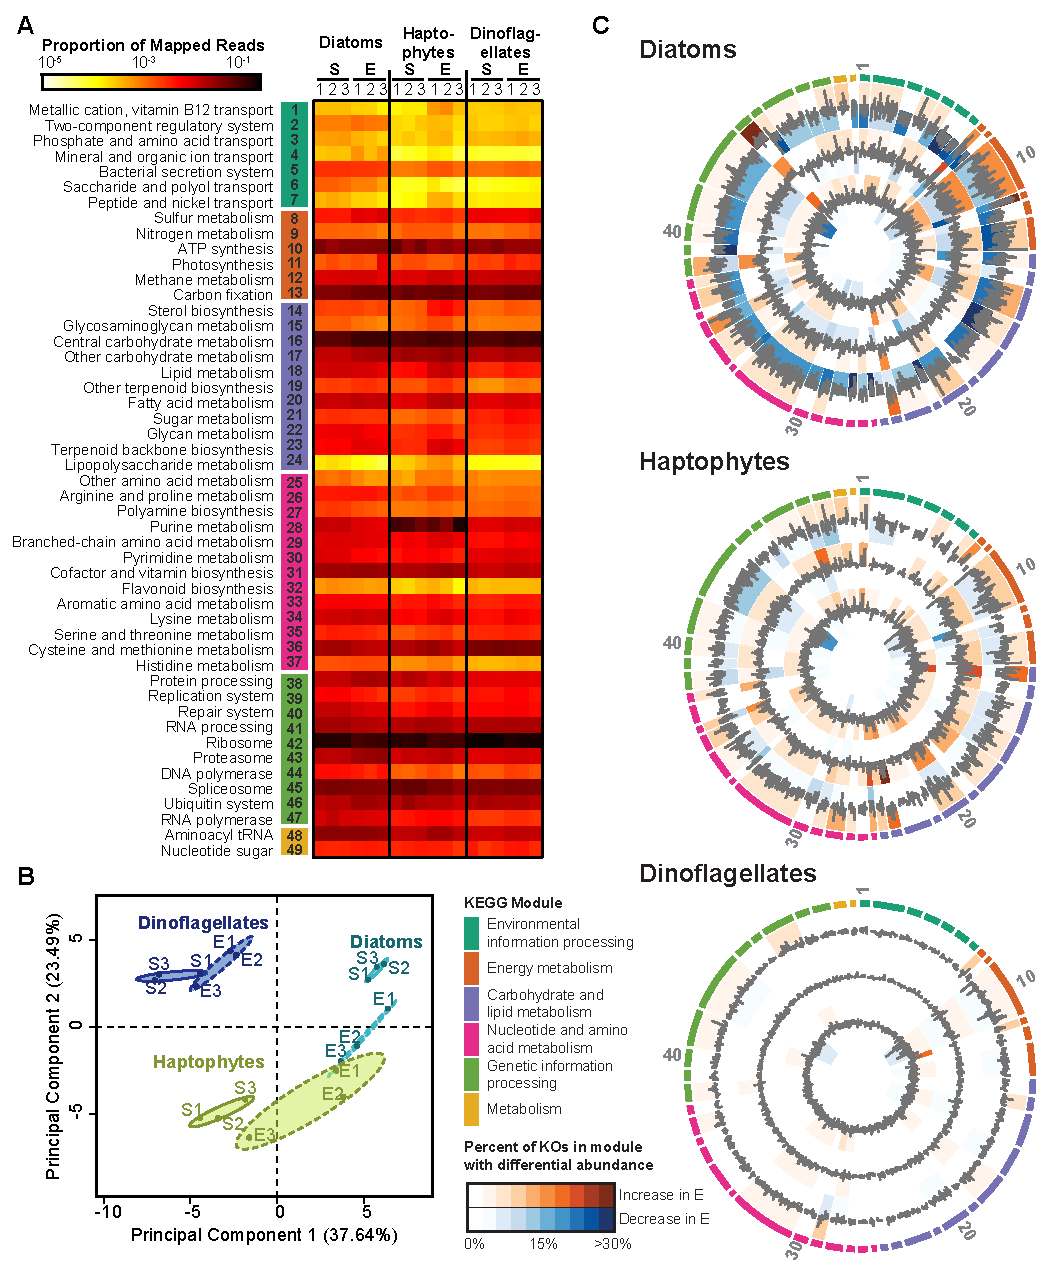
\includegraphics[width=1.1\textwidth]{Images/C4_Figure2_Final.png}}
    \caption[Quantitative metabolic fingerprint (QMF) and patterns of differential expression across KEGG orthology following DSW addition underscore functional group traits]{Quantitative metabolic fingerprint (QMF) and patterns of differential expression across KEGG orthology following DSW addition underscore functional group traits. Caption continued on following page.}
  \label{fig:c4f2}

\end{figure}

\begin{figure}[h!]
    \contcaption{Quantitative metabolic fingerprint (QMF) and patterns of differential expression across KEGG orthology following DSW addition underscore functional group traits. (A) The relative metabolic partitioning of the mRNA pool across the three \textit{in situ} samples (S1-S3) and corresponding deep seawater (DSW) incubation experiments (E1-E3) was assessed using QMF. The summed proportion of mapped reads falling into each of the KEGG modules is depicted as a heat map. (B) Principal component analysis of the QMF signals for each of the functional groups across S1-S3 and E1-E3; 95\% confidence ellipses are indicated for each of the sample types by functional group. (C) Log fold change and significance of differential expression between deep seawater (DSW) amendments and \textit{in situ} samples for KEGG orthologs is visualized with Circos \citep{Krzywinski2009} for the diatoms, haptophytes, and dinoflagellates. Outermost ring colors indicate the KEGG super module, with individual wedges of the pie corresponding to KEGG modules as numbered in A. Concentric circles indicate the expression of the three, replicated DSW addition experiments compared to \textit{in situ} samples: E3 (outer), E2 (middle), E1 (inner). The log fold change of individual KEGG orthologs is depicted as a bar plot bounded -3 to 3. The background color of individual KEGG modules identifies the percentage of genes within module that were significantly (2 fold-change, post-$p > 0.95$) increased (orange) or decreased (blue) in abundance, where darker colors indicate that a higher percentage of genes within that module were significantly different.}
\end{figure}


The static nature of population structure and functional group QMF was altered by replicated nutrient-rich DSW addition experiments, which led to a 7- to 17-fold increase in chlorophyll a, increases not observed in the control treatment (Figure \ref{fig:a4f1}). This increase was consistent with previous studies, which also noted increases in diatoms \citep{McAndrew2007}. Diatom-associated mRNA reads increased in each of the DSW experiments (Figure \ref{fig:c4f1}A). Although species designations can be influenced by the composition of the database used for read mapping, apparent taxonomic shifts occurred at the species-level for diatoms and haptophytes (Figure \ref{fig:a4f2}). Shifts in taxonomic composition were consistent with DSW addition for diatoms and haptophytes, with rank abundance clustering for all experiments (Figure \ref{fig:c4f1}B).  Taxonomic shifts in diatoms were driven by an increase in the rank abundance of certain species, which in all cases were pennate forms (Figure \ref{fig:a4f2}), including genera known to be present in the NPSG like Pseudo-nitzschia \citep{Silver2010} and common in oligotrophic nutrient amendment incubation studies \citep{Marchetti2005, Marchetti2012a}. Although species shifts also occurred within the haptophtyes, \textit{Emiliania huxleyi} was always the most dominant taxon (Figure \ref{fig:a4f2}). The shifts in diatom dominance compared to the consistent dominance of \textit{E. huxleyi} may reflect differences in evolutionary strategies, with metabolic diversity spread across many species in the diatoms and a single species complex with a pangenome, \textit{E. huxleyi}, in the haptophytes \citep{Read2013}. The QMF of DSW addition was significantly different from the QMF of the in situ community for both diatoms and haptophytes, but not dinoflagellates (Figure \ref{fig:c4f2}B). Following DSW addition, the QMF for both diatoms and haptophytes was characterized by increased expression of modules associated with growth, such as carbon fixation (Figure \ref{fig:c4f2}A). These shifts are not the result of changes in species composition, as the patterns of expression from individual species tracked the summed community (Figure \ref{fig:a4f3}). The lack of change in the QMF of dinoflagellates (Figure \ref{fig:c4f2}B) likely reflects their range of life strategies \citep{Hackett2004} and minimal transcriptional regulation of gene expression as observed in culture-studies \citep{Moustafa2010}. \par

%Figure 3

\begin{figure}[h!]
  \centering
    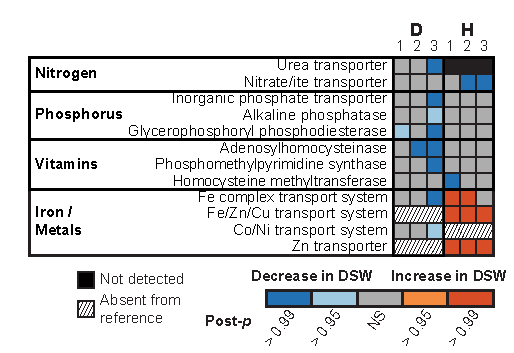
\includegraphics[width=.8\textwidth]{Images/C4_Figure3_Final.pdf}
    \caption[Shifts in transcript abundance of genes responsive to biogeochemical forcing]{Shifts in transcript abundance of genes responsive to biogeochemical forcing. The significance of changes in abundance (2 fold-change, post-$p > 0.95$, or $>0.99$) for genes known to be associated with N, P, vitamin, Fe, or other trace metals metabolism for diatoms (D) or haptophytes (H) is indicated as blue (decrease) or orange (increase). Genes present within the reference transcriptome, but not detected in the field were marked in black, and genes absent from the reference are hashed. KEGG IDs are as follows: Urea transporter (K11959), nitrite/ate transporter (K02575), phosphate transporter (K08176), glycerophosphoryl diester phosphodiesterase (K01126), adenosylhomocysteinase (K01251), phosphomethylpyrimidine synthase (K03147), 5-methyltetrahydrofolate-homocysteine methyltransferase (K00548), iron complex transport system (K02013), iron/zinc/copper transport system (K11706), cobalt/nickel transport system (K02006), zinc transporter (K14715).}
  \label{fig:c4f3}
\end{figure}


Variability within the QMF modules was resolved by statistically assessing the changes in abundance of individual genes for each functional group using a Bayesian approach \citep{Wu2010} (Figure \ref{fig:c4f2}C, Figure \ref{fig:a4f4}). Statistical significance (2-fold change, posterior probability (post-$p$) > 0.95) of differential abundance was examined for 4038 KEGG orthologs common to diatoms, haptophytes, and dinoflagellates. As with the QMF (Figure \ref{fig:c4f2}A), dinoflagellates demonstrated little to no significant changes in gene expression (Figure \ref{fig:c4f2}C). The suites of transcripts with significantly increased transcript abundance following DSW were highly conserved for both diatoms and haptophytes across the three replicate experiments (40\% of 334 and 19\% of 490 genes common, respectively) but differed between functional groups (41 of the total 824 significantly increased transcripts genes common) (Figure \ref{fig:a4f5}). Of the genes with increased transcript abundance many of those conserved across all three experiments for diatoms and haptophytes were associated with growth (e.g. ATP synthesis (10), photosynthesis (11), and carbon fixation (13)) (Figure \ref{fig:c4f2}C, Fig S5). Additionally, following DSW addition, diatoms had signals indicative of the incorporation of both nitrogen (increasing abundance of glutamate and glutamine synthase) and iron (switching from NADPH to ferredoxin sulfate reductase). These changes in transcriptional patterns indicate that both diatoms and haptophytes increase fundamental metabolic processes required for photosynthetic growth in response to DSW. \par
For diatoms and haptophytes, the consistency in genes with increased transcript abundance stands in contrast to the patterns of genes with significantly decreased transcript abundance following DSW addition (Figure \ref{fig:a4f5}). Diatoms were typified by significant decreases in transcript abundance of many genes following DSW, consisting of a large portion (1389 genes) of their metabolism compared to haptophytes (490 genes) (Figure \ref{fig:c4f2}C). Genes with decreased transcript abundance were variable across the three experiments (1.5\% and 6.9\% similar for diatoms and haptophytes, respectively) (Figure \ref{fig:a4f5}) and imply a tailoring of basal metabolism to the change in biogeochemical environment from DSW amendment. Across the KEGG modules, specific genes known to be markers of nutrient limitation significantly decreased in abundance following DSW addition (Figure \ref{fig:c4f3}), potentially signifying a limitation in the in situ population that was alleviated following resupply. Such genes or their protein products are frequently used as proxies to identify limitation in the field \citep{Saito2014}. In E1 and E2, there was a decrease in diatom-associated glycerophosphoryl phosphodiesterase \citep{Dyhrman2012} and adenosylhomocysteinase \citep{Bertrand2012a}, indicative of phosphorus (P) and vitamin limitation, respectively (Figure \ref{fig:c4f3}). Silica transporters, though not in KEGG, were surveyed and not found to have significant shifts in abundance. E3 was characterized by a decrease in abundance of many genes indicative of limitation in the diatoms, including but not limited to, a urea transporter \citep{Bender2012}, a phosphate transporter \citep{Dyhrman2012}, and metal transporters (Figure \ref{fig:c4f3}). This is suggestive of diatom co-limitation in E3, similar to patterns of co-limitation recently observed in picocyanobacteria in the Pacific Ocean \citep{Saito2014}. There was a decrease in transcript abundance for haptophyte-associated nitrate and nitrite transporters in E2 and E3 and homocysteine methyltransferase in E1 (Figure \ref{fig:c4f3}). This may be indicative of nitrogen and vitamin limitation based on the pattern in other organisms \citep{Bertrand2012a, Bender2014}, but the regulation of these targets in haptophytes is poorly understood. Metal transport proteins were significantly increased for haptophtyes in E1-E3 and indicated metabolic strategies following the addition of resources that differ from diatoms. In contrast to the diatoms, no markers of P limitation, such as the phosphate transporter or alkaline phosphatase in \textit{E. huxleyi} \citep{Dyhrman2006, Dyhrman2003, Xu2006}, were significantly decreased for haptophytes, consistent with their known tolerance for P limitation \citep{Lessard2005}. These data evince that diatoms and haptophytes are not under the same biogeochemical controls in situ and employ disparate strategies following DSW addition to capitalize on newly available resources. Being able to identify and characterize multiple markers of limitation in a genera-specific manner for these eukaryotes is of central importance to the modeling of aperiodic blooms of these groups in oligotrophic systems. \par 



%Figure 4
\begin{figure}[p!]
  \centering
    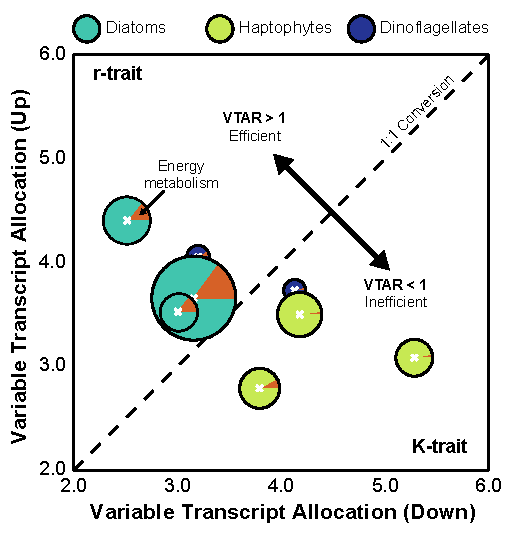
\includegraphics[width=.8\textwidth]{Images/C4_Figure4_Final.pdf}
    \caption[Variable transcript allocation space differentiates functional group strategies]{Variable transcript allocation space differentiates functional group strategies. The variable transcript allocation score (Equations \ref{eq:c4e3} and \ref{eq:c4e4}) of the genes with significantly increased ($VTA_{Up}$) or decreased ($VTA_{Down}$) abundance in the deep seawater (DSW) amendment relative to the \textit{in situ} sample is plotted for diatoms, haptophytes, and dinoflagellates for E1-E3. The size of the pie indicates the total number of genes with significantly different transcript abundances between the \textit{in situ} and DSW amended treatments. The proportion of increased TPM in E within the energy metabolism super group is illustrated as a pie slice in orange.}
  \label{fig:c4f4}
\end{figure}



The above analyses focus primarily on the gene content and transcriptional patterns; however, the underlying eco-evolutionary metabolic traits for a functional group may be better described by considering the shift in the total transcript pool (TPM). Using the statistically resolved patterns of increases and decreases in transcript abundance, a variable transcript allocation ratio ($VTAR$) was calculated to model functional group transcriptional responsiveness to DSW amendment (Figure \ref{fig:c4f4}). $VTAR > 1$ indicates an efficient reallocation of the transcriptional potential from genes with decreased abundance to genes with increased abundance following DSW amendment, while $VTAR < 1$ indicates an inefficient reallocation. The dinoflagellates had variable $VTA$ scores due to their small pool of differentially abundant genes, however the $VTA$ scores consistently resulted in disparate patterns for the diatom and the haptophytes (Figure \ref{fig:c4f4}). In every experiment, the diatoms fell above the 1:1 line, with a $VTAR > 1$ ($1.15 - 1.75$), while haptophytes fell below, with a $VTAR < 1$ ($0.58 - 0.83$) (Figure \ref{fig:c4f4}). The relative efficiency of reallocation, here defined by $VTAR$, reflects differences in the metabolic traits of these functional groups and aligns with preexisting ecological traits as defined by \citep{Margalef1978}. Diatoms are r-selected with high maximum uptake rates that enhance their competition under high or fluctuating nutrients (such as a DSW upwelling event). This trait is reflected in the significant decrease in transcript abundance of many genes across a broad metabolic range coupled with the targeted increase of a subset of genes largely falling within the energy metabolism super module (Figure \ref{fig:c4f4}), a pattern which was also observed with gene-focused analyses using trimmed mean of M value (TMM) normalization \citep{Marchetti2012a, Robinson2010} (Figure \ref{fig:a4f6}). Haptophytes are K-selected, possessing a low half-saturation constant that enhances growth under low nutrient conditions, but are unable to capitalize on nutrient pulses like r-selected competitors. Again, this ecological trait is reflected in changes in the haptophyte transcript pool. Though numerically fewer of their genes significantly decreased in abundance with DSW addition, the total TPM represented by those genes with decreased abundance exceeded that of those induced, defined by $VTAR <1$ (Figure \ref{fig:c4f4}). This is also reinforced by the gene-specific analysis (Figure \ref{fig:a4f6}). It has been speculated that the mechanistic basis for the r- and K- tradeoff dichotomy in the phytoplankton lies in the disparate investment in growth or resource acquisition machinery \citep{Litchman2008}. The large portion of the transcript pool that increased ($VTAR > 1$) for diatoms shows an ability to capitalize on newly available resources, with 14.2-14.9\% of the increased TPM in the KEGG energy metabolism super module (Figure \ref{fig:c4f4}). 
Haptophytes ($VTAR < 1$), by contrast, do not efficiently reallocate the transcript pool, with only 5.5-10.2\% of the increased TPM in energy metabolism (Figure  \ref{fig:c4f4}). In short, haptophytes do not appear to modulate their transcript pool to capitalize on growth processes as efficiently as diatoms (Figure  \ref{fig:c4f4}). \par



These functional group-specific molecular and metabolic mechanisms underpin the aperiodic eukaryotic phytoplankton blooms in the oligotrophic ocean. Whereas both diatoms and haptophytes, including calcifying groups, likely contribute to a shift towards a net autotrophic condition when there is a nutrient pulse, the ecosystem function of oligotrophic systems may ultimately hinge on the unique trait of the diatoms to more efficiently turn over their scavenger metabolism to one of enhanced production. This finding is consistent with the dominance of diatom-associated BSi export relative to PIC export during summer in the NPSG \citep{Karl2012}. Unlike the preceding 13 years of study at Station ALOHA \citep{Karl2012}, enhanced production and export characteristic of bloom events were not observed during the summer of 2012, which exhibited a period of sustained net-heterotrophy. We demonstrated through simulated blooms that the metabolic capacity for enhanced production is inherent in the large eukaryotic phytoplankton regardless of water mass, suggesting that the lack of bloom in 2012 was variably due to deficiency in macronutrients, vitamins, and metals. As the conditions observed during summer 2012 may be increasingly encountered in a future ocean \citep{Doney2012}, modeling the molecular traits and tradeoffs of these populations will help better predict ecosystem state and metabolic balance of the ocean. \par











\chapter{Physiological response and strain variation of the \textsl\textsc{Emiliania huxleyi} species complex under changing nutrient environments}

\raggedbottom


\clearpage

\section{Abstract} 
Phytoplankton are well tuned to respond to changing environments, which may happen at the community-level with functional group succession, at the species-level through shifts in strain composition, or at the strain-level through alterations to phenotype. Community-level shifts have been well described; however, strain or phenotypic shifts have been more difficult to identity and describe in the field. Here, we examined the intersecting roles of metabolic plasticity and strain diversity in the response of natural populations of the biogeochemically significant cocolithophore \textit{Emiliania huxleyi} to shifting nutrient regimes in the North Pacific Subtropical Gyre (NPSG). Using a metatranscriptomic approach, field observations were paired with microcosm studies to track the compositional and metabolic responses to shifts in the geochemical environment. The transcriptomes and genome of five strains were clustered based on protein homology to identify the `core' set of genes common across strains, as well as sets of genes unique to each strain. These strain-specific gene sets were used to track strain composition in the field and microcosms. The strain composition of the \textit{in situ} samples varied little over the sampling period, with transcripts specific to strains CCMP1516, CCMP370 and PLYM219 being the most abundant.  Following the addition of nitrogen, however, transcripts specific to strains CCMP374 and CCMP379 exhibited dramatic increases. In addition to the variations in strain diversity observed following nutrient addition, significant changes in transcript abundance were observed for gene pathways involved in nitrogen, and phosphorus metabolism.  The data suggest that nitrogen is a major driver of the physiological ecology of \textit{E. huxleyi} in this system, and nitrogen supply may be linked to shifts in the ploidy of the population and changes in both nutrient physiology and calcification state. Together, these data underscore the ecological importance of the ``pan genome'' of \textit{E. huxleyi}, suggesting that genetic variability within the species complex combined with global metabolic plasticity may be at the heart of its success in a wide variety of marine environments. \par

 


\section{Introduction}
Central to the carbon cycle, marine phytoplankton are estimated to constitute nearly half of global primary productivity \citep{Field1998}. Beyond their contributions to primary production (1-10\% of total marine carbon fixation), cocolithophores are an important source of particulate inorganic carbon in the form of calcite (CaCO$_{3}$) and are estimated to comprise about 50\% of calcite deposition to sediments \citep{Poulton2007}. Consequently, cocolithophores play a dual role in the cycling of carbon, both in the organic carbon pump, drawing CO$_2$ out of the atmosphere, and the carbonate counter pump, where CO$_{3}^{2-}$ removed for calcification increases total alkalinity thus leading to a positive feedback on atmospheric pCO$_2$ \citep{Zondervan2002}. The ratio of calcification to carbon fixation has been found to vary across environmental factors such as temperature, salinity, light and nutrients \citep{Paasche2001, Bollmann2007, Zondervan2007, Feng2008}. \par

Numerically, \textit{Emiliania huxleyi} is the most abundant cocolithophore species in the modern ocean \citep{Paasche2001}, known for its cosmopolitan distribution and ability to form large blooms in both eutrophic coastal regions and oligotrophic open ocean regions \citep{Holligan1993, Brown1994}. \citet{Margalef1978} put forth a hypothesis that such blooms by cocolithophores (K-selected) follow upon the boom-bust dynamics of diatoms (r-selected), where diatoms bloom quickly depleting the environment of key nutrients such as nitrogen (N), phosphorus (P), and silica (Si). In these low nutrient environments, it is frequently \textit{E. huxleyi}, which is thought to be the most r-selected of the cocolithophores, that thrives and blooms \citep{Litchman2006}. \textit{E. huxleyi} is known to be well-adapted to such low-nutrient environments, having the ability to alter its metabolism to scavenge nutrients from organic compounds \citep{Palenik1997, Dyhrman2003, Bruhn2010, Rouco2013}. This metabolic plasticity may be central to its ability to adapt to the environment and form large blooms.\par

The potential effects of rising atmospheric CO$_2$ \citep{Raven2005, Meinshausen2011} on the production and calcification of this keystone phytoplankton group is debated and has been found to vary both across environmental parameters, such as the nutrient environment \citep{Sciandra2003, Leonardos2005, Rouco2013}, and amongst strains \citep{Riebesell2000, Iglesias-Rodriguez2008, Langer2009}. Beyond the variable response to carbonate chemistry, inter-strain variability has been observed in the ability to grow on various organic substrates \citep{Strom2009} and in enzymatic activities \citep{Steinke1998, Dyhrman2003, Alcolombri2015}. The capacity for this variability was largely revealed through the genome sequencing of many \textit{E. huxleyi} strains \citep{Read2013}. Historically believed to be a single species, the genome of \textit{E. huxleyi}, termed a ``pan genome'', was found to be highly variable across strains, not only in microsatellite regions, but in gene content, with up to 25\% coding regions variable across species \citep{Read2013}. Such genomic variability has been described in a cosmopolitan cyanobacterial species \citep{Kashtan2014} and may be central to the success of these species in diverse environmental conditions \citep{Biller2014}, but had not been previously described for a marine microeukaryote. While significant diversity as described by non-coding microsatellite loci has been observed in the field \citep{Iglesias-Rodriguez2006}, the variability of gene content as seen across various isolates has not been directly observed \textit{in situ}. Global surveys of mixed communities have suggested that the known diversity of \textit{E. huxleyi} may be a cornerstone of its future response to changing ocean conditions (e.g. increased stratification and acidification) \citep{Beaufort2011}.\par

In spite of the intersecting importance of metabolic plasticity and strain diversity in the ecology of \textit{E. huxleyi}, these dynamics have not yet been assessed in the field, being primarily limited to monoculture studies of individual isolates. Using a metatranscriptomic approach, the relative contribution and activity of different strains of \textit{E. huxleyi} and their combined physiological signature were tracked both \textit{in situ} in the North Pacific Subtropical Gyre and under altered nutrient conditions through replicated microcosm incubations.  \par



\section{Materials and Methods}

\subsection{Sample collection and shipboard nutrient incubation experiments}
Seawater for the \textit{in situ} eukaryote community mRNA analysis was collected at the HOT, Station ALOHA ($22^\circ 45^\prime$ N, $158^\circ 00^\prime$ W) from a depth of 25 m at 1400 hrs (local time) on six occasions during the summer of 2012 (S1: 6 August, S2: 12 August, S3: 24 August, S4: 30 August, S5: 2 September, S6: 5 September) using a Eulerian sampling scheme as part of the HOE-DYLAN research expedition as per \citet{Alexander2015a}. Water was collected in acid-washed 20-L carboys and approximately $60 L$ of seawater was prescreened through $200 \mu m$ mesh and then filtered onto polycarbonate filters ($5.0 \mu m$ pore size, $47 mm$, Whatman) by way of peristaltic pump. Filters were changed every 20 minutes or when flow rate decreased. Filters were placed in cryovials and stored in liquid nitrogen until mRNA extraction. The total length of filtration time did not exceed 3 hours. \par

In conjunction with these field-based surveys, two factorial nutrient amendment incubation experiments focused on the macronutrients N and P were performed with natural communities (T$_0$ of E1 was S1 and T$_0$ of E2 was S4) (STable 1). Incubations were modeled after a simulated 10\% deep seawater (DSW) upwelling as described in \citet{Alexander2015a} and designed to tease apart the potential nutritional components of DSW upwelling. The concentration of iron was modeled after \citet{Marchetti2012a} and vitamin B\textsubscript{12} was modeled after \citet{Bertrand2007}. Triplicate 20-L carboys of each treatment were incubated at 30\% surface light-levels using on-deck incubators for 7 days and processed as described above, on the final day at 1400 hrs (local time). Nutrient concentrations for phosphate [PO$_{4}$], nitrate and nitrite [NO$_2$+NO$_3$] were measured by filtering $125 mL$ of seawater through a $0.2 \mu m$, $47 mm$ polycarbonate filter, and stored frozen (-$20^\circ$C) in acid washed bottles until analysis at the Chesapeake Bay Lab at the University of Maryland according to the facility's protocols. Samples for alkaline phosphatase activity (APA) were collected by filtering 250-ml of whole seawater onto polycarbonate filters ($0.2 \mu m$ pore size, $47 mm$, Whatman) and frozen at -$20^\circ$C. These filters were then resuspended in artificial seawater and assayed for APA fluorometrically using the fluorogenic phosphatase substrate 6,8-difluoro-4-methylumbelliferyl phosphate (diMUF-P, Molecular probes) following established field protocols \citep{Dyhrman2006}. Chlorophyll a was measured on whole water samples collected onto GF/F filters ($25 mm$, Whatman) using a 90\% acetone extraction and assayed by fluorescence using the AquaFluor Turner TD700 \citep{Parsons1984}.\par

\subsection{RNA extraction and sequencing}
RNA was extracted from individual filters with the RNeasy Mini Kit (Qiagen), following a modified version of the yeast protocol. Briefly, lysis buffer and RNA-clean zirconia/silica beads was added to the filter and samples were vortexed for 1 minute, placed on ice for 30 seconds, and then vortexed again for 1 minute. Samples were then processed following the yeast protocol. The resulting RNA was eluted in water and then treated for possible DNA contamination using TURBO DNA-free Kit (Ambion) following the Rigorous DNase protocol. RNA from individual filters was then pooled by sample, using the RNA Cleanup Protocol from the RNeasy Mini Kit (Qiagen). The resulting RNA sample thus represented approximately $56 L$ of total seawater for the \textit{in situ} sample. Filters were pooled across like triplicate bottles by treatment, totaling $56 L$ from each of the incubation treatments. The total RNA sample was then enriched for eukaryotic mRNA through a poly-A pull down. The resulting enriched mRNA sample then went through library preparation with the Illumina TruSeq mRNA Prep Kit (Illumina). Libraries were sequenced with the Illumina HiSeq2000 at Columbia Genome Center (New York, NY). Each sample was sequenced to produce a targeted 60 million, 100 base pair, paired end reads. Raw sequence data quality was visualized using FastQC and then cleaned and trimmed using Trimmomatic v 0.27 (paired end mode; 6-base pair wide sliding window for quality below 20; minimum length 25 base pair). 
\subsection{Community- and strain-specific mapping and expression analysis}
Transcriptome sequences and annotations generated through the Marine Microbial Eukaryote Transcriptome Sequencing Project (MMETSP) that were made public as of 17 March 2014 were collected and treated as per \citet{Alexander2015a} to track species composition of the metatranscriptomes. Due to the large size of the resulting MMETSP database, trimmed reads from the metatranscriptome were mapped to the MMETSP using the Burrows-Wheeler Aligner \citep{Li2010} (BWA-mem, parameters: -k 10 -aM) and then counted using the HTSeq 0.6.1 package \citep{Anders2014}. \par

The combined transcriptomes (as assembled from the NCGR on 4 September 2013) from unialgal cultures of \textit{Emiliania huxleyi} strains CCMP374 (MMETSP1006-MMETSP1009), CCMP379 (MMETSP0994-MMETSP0997), CCMP370 (MMETSP1154-MMETSP1157), and PLYM219 (MMETSP1150-MMETSP1153). All transcriptome assemblies used are available through the iMicrobe data commons. Additionally, the predicted transcripts from the \textit{E. huxleyi} genome, strain CCMP1516, were used. All transcriptomes were trimmed based on predicted peptide length, requiring sequences be longer than 70 amino acids. The resulting set of genes was considered for subsequent analyses. Peptide sequences were clustered into gene clusters with orthoMCL \citep{Li2003}, using standard parameters: BLASTP with an e-value cutoff of 1e-5, and an inflation value (-I) of 1.5. Initially, the transcripts unique to CCMP1516, here surveyed using the predicted transcripts from the genome, were the most dominant of the subsets of genes in these analyses, representing ~50\% of the \textit{E. huxleyi} reads in the field (Supplemental Figure Core Changes). Closer inspection demonstrated that many of the most highly represented genes identified as unique to CCMP1516 were associated with metabolic stasis or senescence (e.g. OG1\_5\_1124, a group of homologous proteins in the \textit{E. huxleyi} genome such as JGI \#413698 annotated as putative senescence-related proteins and highly expressed in all field samples). Many of the proteins in the unique set of CCMP1516 were identified as ``core'' amongst the 13 strains surveyed by \citet{Read2013}, yet were absent in some or all of the transcriptomes of the four strains in this study. This absence likely is related to the fact that these strains were largely sampled under exponential growth conditions, limiting the expression of genes that might be associated with stressors or stasis. The lack of `core' gene representation in some of these transcriptomes underscores the importance of growth condition in transcriptome completeness.\par

Using this clustering framework, field and incubation samples were mapped to the data set using RSEM, a software package designed to estimate gene and isoform expression values from RNA-seq data. Here we define orthologous groups as genes and individual transcripts (from any strain) as isoforms. Data were mapped using RSEM version 1.2.20 (parameters: --paired-end -p8 -bowtie2 -bowtie2-mismatch-rate 0.2)\footnote{A note: RSEM is not yet able to deal with gapped mapping, such as enabled by bwa, which was used for the community-level mapping due to database size constraints.}. Taking a conservative approach, the RNA abundances from like treatments (each consisting of pooled triplicate bottles), which were run with different communities from separate water masses more than two weeks apart, were considered to be biological replicates for differential abundance analysis. These analyses were run with edgeR using default parameters to calculate dispersion and to assess differential abundance of both individual transcripts and orthologous groups of each of the amended incubations compared to the no-addition control. Looking to previous literature, genes thought to be associated with nitrogen and phosphorus metabolism \citep{Dyhrman2006, Rokitta2014, McKew2015} and with calcification and ploidy state \citep{VonDassow2009, Mackinder2011, Frada2012} were compared against the translated proteins comprising the orthologous groups used in this study (tblastn with an e-value cutoff of 1e-20).\par



\section{Results and Discussion}

Total mRNA ($>5.0 \mu m$) from the surface mixed layer at Station ALOHA in the NPSG was deeply sequenced six times during the summer of 2012, following a Eularian sampling scheme. To perturb the nutrient environment of the community, two identical microcosm incubation experiments were conducted with natural populations approximately two weeks apart. These experiments included a no addition control, a 10\% (v/v) deep ($700m$) seawater (DSW) treatment to simulate upwelling, and four treatments designed to skew the nitrogen (N) : phosphorus (P) ratio (Supplemental Table Nutrients Added, Supplemental Figure Nutrient Concentrations TF). Sequence reads from the \textit{in situ} and experimental treatments were conservatively mapped to a custom database comprised of all publicly available transcriptomes in the Marine Microbial Eukaryotic Transcriptome Sequencing Project (MMETSP) \citep{Keeling2014}. Data were also mapped separately to a curated set of available \textit{E. huxleyi} transcriptomes \citep{Keeling2014}) and to the genome \citep{Read2013} encompassing five genetically distinct strains: CCMP1516, CCMP370, CCMP374, CCMP379, and PLYM219 (Supplemental Table, Strain information).\par


\subsection{Diatom and haptophyte community structure}

The taxonomic composition of the RNA pool was used to examine diatom and haptophyte populations over time and in the microcosms. Population structure, as measured with Spearman rank abundance, was stable across all \textit{in situ} samples for both the haptophytes and the diatoms (Figure 1A). Following N-addition, however, a distinct shift in the population structure of diatoms and haptophytes occurred, with treatments to which N was added (+N, -P, +DSW) clustering separately from those to which no N was added (\textit{in situ}, control, +P, -N) with UPGMA distance between the two clusters of 0.45 and 0.5 for diatoms and haptophytes, respectively (Figure 1A). In diatoms, clustering was also observed between treatments to which trace metals were added in addition to N (-P, +DSW) compared to treatments to which only N was added (UPGMA distance of 0.28) (Figure 1A). This pattern was not observed in haptophytes, where the -P treatments clustered separately from the +N and +DSW treatments (Figure 1A). Following N-addition there was an increase in RNA reads associated with \textit{Emiliania} relative to its abundance in the control, but no other haptophyte became the most abundant (Figure 1C, D). While \textit{E. huxleyi} was consistently the most abundant haptophyte (Figure 1C, D), the dominant diatom changed from Pseudo-nitzschia to Cylindrotheca when N and trace metals were both added (Figure 1C, D). This pattern was strikingly consistent across both microcosms separated in time by several weeks (Fig). The importance of Si and Fe in the structuring of diatom populations is well-documented \citep{Marchetti2005, Marchetti2012a}, and here treatments containing N and Fe are clearly driving changes in diatom rank abundance at the genus level. A similar pattern was not observed within the haptophytes, where \textit{E. huxleyi} was consistently the most abundant. The strain diversity as manifest in the pan genome of \textit{E. huxleyi} \citep{Read2013} may be central to the observed dynamics between haptophytes and diatoms, with strains in \textit{E. huxleyi} playing a similar role to the genus in diatoms.\par


\subsection{\textit{E. huxleyi} species-complex physiological ecology}

Clustering of orthologous proteins was used to isolate the transcript signals from different \textit{E. huxleyi} strains in the field and examine strain-specific physiological ecology. From the five strains isolated across the world's oceans (Figure 2A) there were a total of 132,888 predicted transcripts (Supplemental Table Strain details). Despite the variable isolation locations, the gene content of these strains covered the same major functional classes with similar relative abundances at the broad level of the KOG class (Supplemental Figure KOG distribution). Grouping these transcripts based on predicted protein homology using OrthoMCL \citep{Li2003} yielded 56,647 distinct orthologous groups. Orthologous groups varied in size and strain representation, with some groups containing proteins from a single strain and some groups having representative proteins from each of the five strains surveyed here (Supplemental Figure Strain groupings). To better understand the physiology of the \textit{E. huxleyi} species complex, metabolic pathways putatively related to N, P, calcification, and ploidy were tracked for both the `meta' organism (sum of all strains -- orthologous group) and for individual strains. \par

Taking a conservative approach, the two replicated experiments, which were performed two weeks apart with different initial communities, were considered as biological replicates. Using these biological replicates, the significance of differential abundance was assessed for each of the orthologous groups and individual gene orthologs in each of the amended incubations compared to the no addition control with edgeR. Genes with a two-fold increase (FDR $< 0.05$) were considered to be differentially abundant. Using this approach, treatments to which nitrate was added (namely, +N, -P, and +DSW) had between 1,212 and 1,466 orthologous groups with FDR $< 0.05$ compared to treatments with no N added that had at most 2 genes significantly differentially abundant (Supplemental Figure Manta). The significantly differentially abundant genes for three treatments that received N were conserved, with 45\% of differentially abundant orthologs common across the three treatments (Supplemental Figure Venn). Far fewer strain-specific transcripts (161 - 918) were identified as significantly regulated (Supplemental Figure Manta). This is likely due to a lack of statistical power, in that the coverage of individual strains was necessarily lower than the whole. Because of this, the following sections focus on the expression of orthologous groups, which consider the global signature of all the strains. However, it is worth noting the wide spread of estimated fold change of individual, strain-specific transcripts compared to the orthologous group (Figure 4). \par


\subsubsection{Nitrogen scavenging and assimilation}

Broadly speaking, genes associated with N-metabolism, which were significantly differentially abundant following N-addition, could be broken into two groups: genes associated with the response to N-limitation and genes associated with the response to newly available substrates, such as ammonium (Figure XA). In microcosm treatments that received N, a number of gene families that are known to be regulated by N supply had decreased abundance.  For example, transporters of organic and inorganic N sources were significantly decreased (FDR $< 0.05$) relative to the no addition control (Figure 4). This included a family of urea transporters (UTP), ammonium transporters (AMT), and nitrate transporters (NRT) (Figure 4; Supplemental Table Genes). In addition to the decreases in UTP, urease (URE), which scavenges N in the form of NH$_{4}^+$ from urea, was significantly decreased following N-addition. Of the N-metabolism genes surveyed, the largest decrease in abundance was observed in three orthologous groups of amidases (AMD) and formamidases (FMD), which scavenge NH$_{4}^+$ from amides and formamides (Figure 4). These patterns were found to persist not only across the two replicated experiments but also across treatments, with many of the genes being significantly regulated in more than one N-amended experiment. \par

There was a strong correlation between the observed patterns of transcript regulation for each of the aforementioned gene families and prior transcriptomic \citep{Rokitta2014} and rate-based \citep{Palenik1997, Bruhn2010} studies focused on N-limitation responses. Most striking, however, is the coordination of each of these markers with a lab-based proteomic study of the physiological response of CCMP1516 to N-limitation (Figure XA) \citep{McKew2015}. The AMT, NRT, and UTP gene families observed to be down in N-amended incubations were each significantly increased in the proteome of N-limited cultures of CCMP1516 (Figure XA).  Additionally, the URE and one of the FMD gene families were found to be up in proteomic analyses (Figure XA). This pattern of regulation in URE was also observed at the transcript level in N-limited cultures of \textit{E. huxleyi}, which may serve as a means of accessing N from the ornithine-urea cycle \citep{Rokitta2015} or as a means of accessing exogenous urea \citep{Dyhrman2003a}. There is a strong literature on the ability of \textit{E. huxleyi} to grow on amides and other organic N sources \citep{Palenik1997}, and evidence of transcript and enzymatic induction of AMD/FMD under N-limiting conditions \citep{Bruhn2010, Palenik1997}. The data from this field study combined with many previous lab-based studies suggest that these N-limitation responses are highly conserved across strains (Figure 3), and across environmental and laboratory conditions as well (Figure 4, X).\par

Beyond the acquisition of N, several markers of changes in N assimilation and energy production were pronounced following the addition of N to the incubations. The NH$_{4}^+$ released by FMD, AMD, and URE is ultimately incorporated into biological material through glutamine synthase (GS) \citep{Rokitta2014}. A shift between the smaller, GS type II, under low N conditions to the larger GS type III with a higher N requirement, following N-addition was observed. In culture transcriptome comparisons, \citet{Rokitta2014} noted that in both haploid and diploid stages, \textit{E. huxleyi} induces a malate:quinone-oxidoreductase (MQO) that can bypass malate-dehydrogenase (MDH) in the TCA cycle and feed electrons directly into the electron transport chain to enable the production of ATP, while limiting carbon loss to respiration. MQO was significantly decreased (between 5 and 9 log fold change) in both +N and +DSW (Supplemental Figure CarbonNucleotideAA). Additionally, though not significantly different, MDH increased 6.4 fold under N-addition (FDR = 0.36) (Supplemental Figure TCA). The MQO, absent from diatom genomes but found to be highly expressed both in N-limited cultures and in this oligotrophic setting, may be a unique and niche-defining aspect of the N-limitation response of \textit{E. huxleyi}. The coordination of the N-induced transporters, enzymes used for the scavenging of N from organic molecules, and shifts in energy metabolism strongly suggest that the \textit{in situ} population of \textit{E. huxleyi} was released from N-limitation with the presence of an added N source, here nitrate.\par

One exception to the coordination observed between the field data with \citet{McKew2015} and other transcriptomic studies \citep{Dyhrman2006, Rokitta2014} were a set of transporters that were significantly increased following N-addition. In each treatment where N was added, three groups of ammonium transporters (AMTs) and a nitrite/formamide transporter (NAR) significantly increased. While an increase of AMT under N-repletion has been observed in centric diatoms \citep{Bender2014}, this shift was likely due to the setting of these experiments. Unlike studies done on axenic cultures, these incubations were performed with whole seawater, consisting of mixed communities of heterotrophic, mixotrophic, and autotrophic organisms. Over the seven day incubation, it is likely that there was active nitrogen fixation \citep{Karl1997} or remineralization \citep{Casciotti2008} that may have produced ammonium or amides. \par

These observations provide an unprecedented glimpse at the import of N in controlling \textit{in situ} molecular physiology of \textit{E. huxleyi} in the NPSG. Moreover, the choreography observed in the patterns of gene regulation between laboratory studies on axenic, monoclonal cultures and field incubation experiments with mixed communities is striking and suggests that these responses are highly conserved within \textit{E. huxleyi}. \par


\subsubsection{Phosphorus scavenging}

The N:P ratio was elevated in the +N, +DSW and -P treatments, the latter of which represented the most extreme condition (Figure Nutrients). Genes associated with P-metabolism, and known to be P-regulated in culture \citep{Dyhrman2006, McKew2015} showed a global trend towards increased abundance following N-addition. The -P condition had more genes changing in P-metabolism than the other treatments, with significant increases observed in genes associated with P-transport, P-scavenging from organic molecules, and polyphosphate (poly-P) metabolism. A family of vacuolar transport chaperonins (VTC), which are thought to be associated with poly-P metabolism \citep{Ogawa2000, Hothorn2009, Dyhrman2012}, had the largest significant fold change in each of the conditions to which N was added (Figure 4). Although poly-P accumulation was thought to be a luxury uptake response \citep{Perry1976}, VTC has been observed to be to be increased in diatoms under P-limitation \citep{Dyhrman2006, Dyhrman2012} and may be indicative of internal poly-P cycling consistent with recent observation of bulk poly-P in the NPSG and the Sargasso Sea (Martin et al. 2014; Diaz et al. 2015). \par

Genes associated with the scavenging of PO$_4$ from organic molecules were also significantly increased, with two glycerophosphoryl diester phosphodiesterase (GDP) orthologous groups and a 5'-nucleotidase (NTD) orthologous group significantly more abundant following N-addition (Figure 4). Additionally, two gene families whose inductions under P-limitation are well-characterized in \textit{E. huxleyi}, alkaline phosphatase (AP1) \citep{Xu2006} and phosphate-repressible phosphate permease (PRPP) \citep{Chung2003, Dyhrman2003, Dyhrman2006}, were significantly increased only in -P (Figure 4). This suggests that P-cycling from organic molecules such as nucleotides (both internal and external) may be central to the low-P-response in \textit{E. huxleyi}. NTD has also been observed to be significantly increased in diatom and pelagophyte metabolism under P-limitation \citep{Wurch2011a, Dyhrman2012}, indicating that this metabolic strategy as seen across diverse taxonomic groups may be a deeply rooted response to P-limitation \citep{Martiny2013}.\par

As with the genes associated with N-limitation, genes associated with P-limitation were well choreographed with the proteomic data from \citet{McKew2015} (Figure XB). Each of the gene families identified as significantly increased in the -P treatment was significantly increased in the P-limited cultures of CCMP1516, with the exception of two gene families, which were likely below their detection limit or lost during the extraction because of membrane association (Figure XB). Notably, NTD, which was not detected by \citet{McKew2015} in CCMP1516, was found to be present in \textit{E. huxleyi} CCMP374 and CCMP373, and induced under P-limitation \citep{Dyhrman2003}. Similarly PRPP has been found to be induced under -P conditions at both the transcript- \citep{Dyhrman2006} and protein-levels \citep{McKew2015}, as well as in cultures grown on organic nitrogen \citep{Bruhn2010}. \par

The regulation of \textit{E. huxleyi} AP1 showed particular sensitivity to the presence of PO$_4$ in the environment (Figure 4B,C). Alkaline phosphatase is a cell surface protein used for scavenging organic P from the environment and its induction in -P is seen in many diverse phytoplankton groups \citep{Sakshaug1984, Dyhrman1997, Dyhrman2003, Wurch2011}. AP1 in \textit{E. huxleyi} has been shown to be increased ~1000-fold at the transcript-level when subjected to P-limiting conditions \citep{Xu2006}, and was found to constitute 3\% of all spectral counts in a P-limited proteomic data \citep{McKew2015}. In +DSW, where the added P was higher than the no addition control, -P, and +N, there was a slight decrease in AP1 transcript abundance. Additionally, bulk community alkaline phosphatase activity (APA) was significantly increased in the -P condition relative to all other treatments (Tukey HSD, $p < 0.05$) and tracked well with the AP1 transcript abundance (Figure XBC). The difference between bulk community activity and transcript abundance in +DSW condition underscores the power of species-specific methods, suggesting that other organisms in the community might be less sensitive to the presence of inorganic phosphate. This falls in line with previous findings that suggest that \textit{E. huxleyi} may have one of the highest affinities (out of the eukaryotic algae) for P, leading to its success in P-limited competition experiments \citep{Riegman2000} and potentially enabling its ability to bloom in P-limited environments \citep{Lessard2005}. Unlike the diatoms, which appear to be co-limited by N and Fe (Figure 1), \textit{E. huxleyi} appears to be primarily limited by N, with a secondary limitation of P. \par


\subsubsection{Shift in life stage and calcification state}

Tracking genes associated with ploidy state and calcification suggests that the community in the NPSG and in non-N-amended incubations were haploid and non-calcifying. The addition of N, however, putatively shifted the community to diploid and calcifying states (Figure 4). Genes thought to be associated with calcification \citep{Mackinder2010} and found to be up-regulated in calcifying cells \citep{Mackinder2011} were found to be significantly increased following N-addition. These genes included those associated with inorganic carbon transport (e.g. carbonic anhydrases (β, γ, δCA) and a group of anion (Cl- / HCO$_{3}^-$) exchangers (AE1)), calcium (Ca) acquisition (e.g. voltage-gated Ca2+ channel (CAV), Na$^+$/Ca$_{2}^+$-K$^+$ exchanger (NCKX), and Ca$_{2}^+$/Mg$_{2}^+$-permeable cation channel (CX)), and proton transport (e.g. Vacuolar H+-ATPase V0 sector subunits c/c (ATPVcc)). Simultaneously in N amended incubations, there was a significant decrease in the abundance of two genes used as markers of haploid life phase \citep{Frada2012}, dynein heavy chain (DYH) and histone H2A (H2A). The life cycle of \textit{E. huxleyi} is thought to fluctuate between diploid and haploid stages, with calcification only occurring in the diploid stage, and motility during the haploid stage \citep{Paasche2001}. The coordinated increase of genes associated with calcification with the decrease of genes associated with haploid life stage, particularly DYH, which is integral to the flagella, highlight this known association of calcification and ploidy state \citep{Frada2012}. The pattern of increased calcification following N-addition also falls in line with previously described coordination between nutrient environment and calcification in \textit{E. huxleyi} \citep{Paasche2001}. P-limitation has been observed to increase Ca content per coccolith and induce calcification in non-calcifying cultures, while N-limitation was found to decrease Ca content per coccolith \citep{Paasche1994, Paasche1998}. The link between ploidy or life phase and nutrient concentration is not well understood \citep{Green1996}, though a connection to viral infection has been hypothesized \citep{Frada2008}. Thus, the predominant state of the \textit{in situ} population of \textit{E. huxleyi} in the NPSG was haploid and non-calcifying in E1 and E2, but shifted with N-addition, suggesting either the strong control of N on the life stage of the population or, potentially, consistent pressure from viruses. 

\subsection{Strain variability with altered geochemistry}

There were 5,243 genes identified as shared amongst the five strains here, fewer than the nearly 20,000 ``core'' genes reported in the comparative genome analysis \citep{Read2013}. To encompass the most comprehensive set of common genes, all proteins identified as `core' by \citet{Read2013} were added to the shared orthologous groups, resulting in 16,914 `core' orthologous groups (Supplemental Figure Core Changes, Figure 2B). This core set accounted for ~80\% of the reads mapping to \textit{E. huxleyi} in the field and ~70\% in incubations (Supplemental Figure Core Changes). The sum of the five sets of genes unique to each of the strains accounted for ~15\% of all transcripts mapped to \textit{E. huxleyi} (Figure 2C). Using the strain-specific orthologous groups as a metric for the relative strain composition in the field (or marker of the most active strain), each of the five strains was detected across the month-long sampling period (Figure 2C).  These data are consistent with the finding that single cells of cosmopolitan taxa isolated from the same environment may possess diverse sets of genetic alleles and flexible gene sets \citep{Kashtan2014}. These results also mirror microsatellite studies of \textit{E. huxleyi} that found high diversity at the global-scale and many genetic polymorphisms between individuals collected in the same sample \citep{Iglesias-Rodriguez2006}. \par

The strain composition of the \textit{in situ} samples varied little over the sampling period. Strains CCMP1516, CCMP370, and PLYM219 had the highest abundances of strain-specific transcripts, while those of CCMP374 and CCMP379 were less abundant (Figure 2C). Although the dominant haptophyte species did not change regardless of nutrient treatment as did the dominant diatom (Figure 1C, D), shifts in the strain-level composition of the \textit{E. huxleyi} were observed. In addition to being dominant in the field, transcripts specific to CCMP1516 and PLYM219 were the most abundant in treatments where N was not added (Control, -N, +P) (Figure 2D, E). By contrast, transcripts specific to both CCMP379 and CCMP374 exhibited dramatic increases (e.g. $<1\% to 5\%$ of reads for CCMP374) following N-addition in both experiments (Figure 2D, E). These shifts may reflect the different capabilities within the original seed population, such as previously observed in strain variability in growth rate on different organic nitrogen substrates \citep{Strom2009} or enzymatic activity (e.g. FMD) \citep{Palenik1997, Bruhn2010}. Given better sequencing coverage, variability between strains in the expression of genes, such as FMD, might have been statistically distinguishable (Figure 4).\par

A subtle difference in the N-amended treatments consistent across experiments, however, was that strain-specific transcripts associated with CCMP379 were more abundant in -P, which had been augmented with iron, trace metals, and vitamins (Figure 2D, 2E). Such enhanced abundance of a particular strain with added trace metals is potentially supported by the heterozygosity observed in trace metal-associated genes \citep{Read2013} and trace metal quotas across strains (Sunda and Huntsman 1992). These results suggest both that multiple strains co-exist in the same environment and that alterations in the geochemical environment can shift the relative abundance and activity of various strains. Such observations support the hypothesis by \citet{Read2013}, who postulated that the diversity in the pan genome as observed across cultured isolates may be present in the field and central to the cosmopolitan nature of \textit{E. huxleyi}. \par

In addition to the observed shifts in strain abundance following changes in the geochemical environment, the expression of the set of 5,243 shared genes (Supplemental Figure Shared Genes) was examined by strain across the nutrient treatments to statistically validate the apparent shifts in strain abundance and transcriptional response. The 5,243 shared gene set was better annotated than the entire set of orthologous groups, with 73\% of the shared orthologous groups annotated with KOG as compared to only 36.9\% for the sum (Supplemental Figure KOG annotation), likely because this set contains essential and well-studied metabolic pathways (e.g. carbon fixation). Focusing on this relatively well-annotated fraction, RSEM \citep{Li2011} was used to estimate the relative contribution of each `isoform', here defined as the orthologous genes from each of the strains comprising the core orthologous group (Supplemental Figure SharedGeneComp). Principle components analysis (PCA) of the estimated TPM of the 5,243 shared orthologous groups, broken down by the five strains across time and experimental condition, showed separation of strains and conditions. The first three components of the PCA explained 36.2\% of the variance (Figure 3). The primary separation occurred along the first component (20.5\% of variance), which clearly separated treatments to which N was added from treatments where no N was added (Figure 3C), similar to shifts observed between functional groups following DSW addition \citep{Alexander2015a}. No difference was seen between strains in the first three components in the treatments to which no N was added (Figure 3A,B). The second and third component separated strains in treatments where N was added, with the second component (8.1\%) separating CCMP1516 from the four other strains and the third component (7.6\%) separating CCMP379 from CCMP374 (Figure 3 B). Interestingly, these data appear tied to the unique gene sets, as the unique gene sets of CCMP379 and CCMP374 were observed to increase in abundance following N-addition (Figure 2). These data suggest that the metabolic profiles of strains based solely on shared genes are similar, at least in the context of this very oligotrophic environment, where haptophytes are thought to be limited \citep{Alexander2015a}. Strikingly, the addition of N appears to change the metabolic profile of all strains in a similar way, e.g. enhanced carbon fixation (Component 1), such as was observed in the strong conservation and choreography of N and P metabolic genes (Figure 4). However, differences between the responses of strains in the shared set of genes exist (Components 2 and 3), paralleling observations of variable response to nutrient pulses across diatom species \citep{Alexander2015}.  \par

With their description of the pan genome of \textit{E. huxleyi}, \citet{Read2013} speculated that the variability in gene content across strains may be indicative of the Bass-Becking hypothesis, or ``everything is everywhere but the environment selects'' \citep{Baas-Becking1934, DeWit2006}, holding true for the strain diversity observed in \textit{E. huxleyi}.  These data from both field observations and incubation experiments demonstrate that a diverse consortium of strains existed simultaneously in the field (Figure 2C). Furthermore, the shift in strain composition or activity in N-amended treatments (Figure 2D,E) may be indicative of the ``environmental selection'' of strains. Cross comparison of the species-specific modulation of the shared gene set also suggests that while there is a strongly conserved response to N-limitation, individual strains respond differently to the same environmental stimuli. \par


\section{Conclusion}

Metabolic plasticity in response to environmental change is a current cornerstone to the study of phytoplankton physiology, with much effort being put towards characterizing transcript- and protein-level shifts following perturbation \citep{Dyhrman2006, Dyhrman2012, Wurch2011, Bertrand2012a, Jones2013, Bender2014, Frischkorn2014}. A compliment to the observed physiological response to the environment in some species has been found to be strain or genomic variability \citep{Kashtan2014}. This study looked at the intersection of these two types of response in field populations of \textit{E. huxleyi} under changing nutrient environments, finding that both strain variability and physiological plasticity are central to the success of \textit{E. huxleyi}. Metatranscriptomic approaches enabled the direct tracking of metabolic shifts in the \textit{E. huxleyi} species complex following changes in the geochemical environment, demonstrating the central role of N in determining the metabolic state of \textit{E. huxleyi} in the NPSG. These analyses suggested that unlike diatoms, which appear to be N/Fe co-limited, P might be secondarily limiting to \textit{E. huxleyi}. In spite of the many factors that separate field and laboratory studies, choreography of the transcriptional response to N- and P-limitation with previous proteomic studies \citep{McKew2015} was observed, suggesting a highly conserved physiological response to these stressors across the species complex. In concert with these observed shifts in physiology, the co-existence of at least five strains in the same environment based on the variable gene sets of each strain was observed. This combined with the modulation of the strain-specific transcript abundance support the hypothesis that the genomic variability of this species complex may facilitate its ability to thrive in a range of environments \citep{Read2013}, such as in other cosmopolitan phytoplankton \citep{Derelle2006, Johnson2006b} inherently limits this type of study and highlights the importance of continued isolation and culturing of phytoplankton strains to facilitate this type of strain-specific study both more broadly in \textit{E. huxleyi}, but also across other phytoplankton groups. \par
Together these direct observations of the shifts in the molecular physiology and the strain composition of natural populations of \textit{E. huxleyi} in response to changes in the geochemical environment suggest that 1) physiological responses to N and P limitation are highly conserved across strains, 2) many strains concurrently exist in the NPSG and 3) fluctuations of environmental parameters may change strain abundances. There is debate as to what level of taxonomic resolution is important in global biogeochemical models \citep{Follows2011}. The results of this study suggest that while strain variability occurs within \textit{E. huxleyi} species complex, the global physiological response to nutrient environments is highly conserved across strains and may be sufficient for accurately capturing the dynamics of this biogeochemically significant taxonomic group.




\chapter{Summary and Conclusions}
\label{chap:6}

\raggedbottom

\textit{``We cannot cheat on DNA. We cannot get round photosynthesis. We cannot say I am not going to give a damn about phytoplankton. All these tiny mechanisms provide the preconditions of our planetary life.'' }

\begin{flushright}-- Barbara Ward, \textit{Who Speaks for Earth?}\footnote{Barbara Ward et al. Edited by Maurice F. Strong. (1973) \textit{Who Speaks for Earth?} New York, Norton. }\end{flushright}



taking these data, I extrapolated what these findings meant to an ecosystem or even global level. In many ways, this sort of extrapolation is incredibly uncomfortable, but 

moleculesconnection to the immense oceanic environment

dove deeply into the molecular physiology and ecology of individual tiny cells living with in a consortium of other tiny cells  

unify an idea that I have been struggling with throughout my PhD

This quote by Barbara Ward

\section{Finding a place for 'omics in a modeling world}

During my PhD it seems that one of the largest hurdles that I have come up against has been trying to figure out how to explain the significance of my work to ocean modelers. The undertone of some of the chapters in this thesis (e.g. Chapter \ref{4}) was that these findings might be easily integrated into biogeochemical models. A

Many of the chapters in this thesis were laced with undertones suggesting that the results from these studies might be easily integrated into biogeochemical models. 

While I am not saying that I think this is a hopeless 

\section{Future Directions}

\section{Conclusions and future directions}
Capitalizing upon this revolution to address biogeochemical or ecological questions, however, is becoming increasingly difficult, as our ability to make measurements has surpassed our ability to analyze, visualize, and compare the data produced.



Barbara Ward, a British economist during the 20\textsuperscript{th} century, was an early, some might say before her time, proponent of sustainable development. She possessed, what I think was, a very holistic view of the intersection of economic and environmental concerns, arguing strongly for humans to practice ``careful husbandry'' of the Earth. Though slightly crass, this quote, aside from hitting somewhat coincidentally upon the major objects of my thesis (phytoplankton, DNA...), neatly sums up a point that I have been struggling with during my PhD. For my research, I dove into the smallest detail, tracking the shifts in RNA composition of a consortium of very tiny organisms living within a very small parcel of water. After analyzing these data, it was hard to figure out a way to connect the results to the global system. These findings at the sub-micro scale seem to detached from the global system to have any real import. But, as Barbara Ward points out, these ``tiny mechanisms provide the conditions preconditions of \textit{our} planetary life.'' 

\appendix
%\renewcommand{\thefigure}{\Alph{chapter}.\arabic{figure}}
\renewcommand{\thetable}{\Alph{chapter}-\arabic{table}}
\chapter{Supplemental Information}

\raggedbottom


%%%%%%%%%%%%%%%%%%%%%%%%%%%

%%%%%%%%%%%%%%%%%%%%%%%%%%%_________________CHAPTERTWO_________________%%%%%%%%%%%%%%%%%%%%%%%%%%%

%%%%%%%%%%%%%%%%%%%%%%%%%%%
\clearpage
\section{Appendix for Chapter 2}
\subsection{Supplemental Figures}
%Supplemental Figure 1: Histogram of TPM distribution
\begin{figure}[h!]
  \centering
    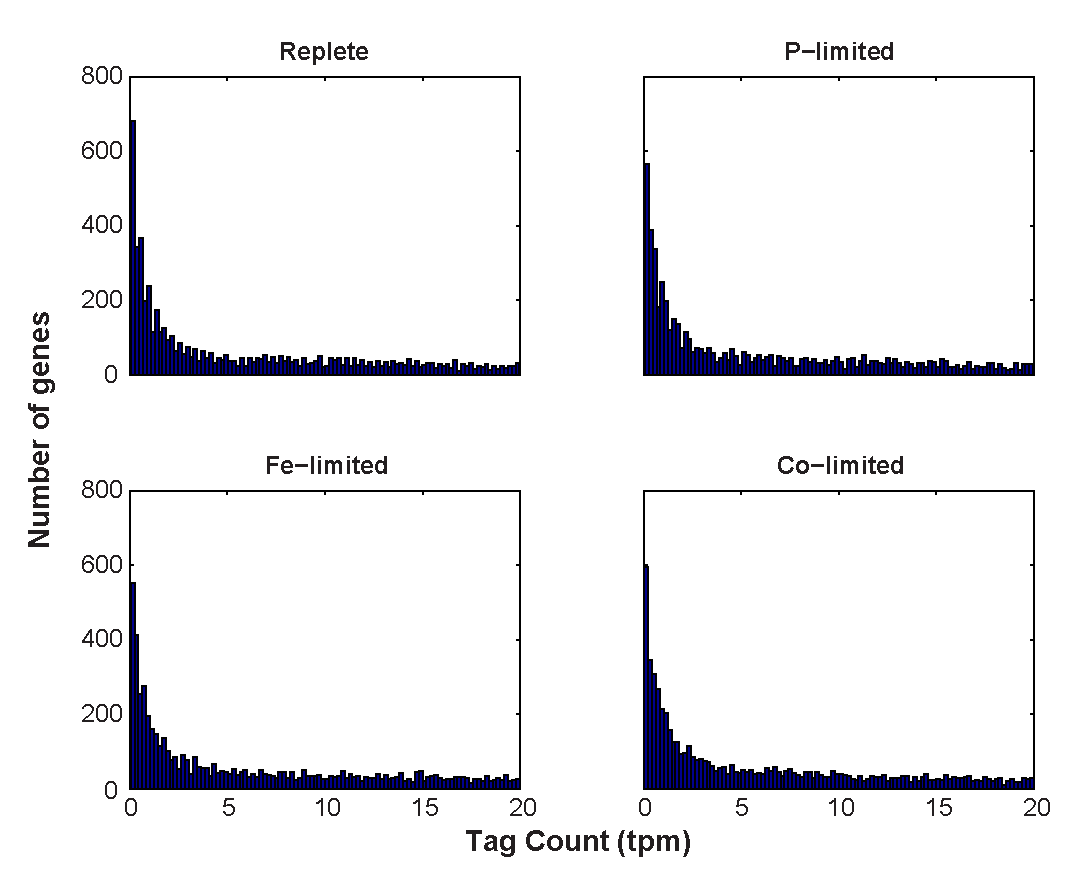
\includegraphics[width=1\textwidth]{Images/C2_FigureS1_v6.pdf}
    \caption[Distribution of normalized tag counts across treatments]{Histogram analysis of the distribution of normalized tag counts (TPM) for each gene across each of the four treatments (Replete, P-limited, Fe-limited, and co-limited). The abundance of normalized tag counts (TPM) was assessed, tallying the total number of genes with a given tag count. Only tag counts less than 20 are depicted to aid the visualization of the inflection in the data at 2.5 TPM.}
  \label{fig:a1f1}
\end{figure}

%Supplemental Figure 2: K-means clusters (all)
\begin{landscape}
   \null         %%<---- this is needed
   \vfill        %%<-----here
   \centering 
    \begin{figure}
    \centering
        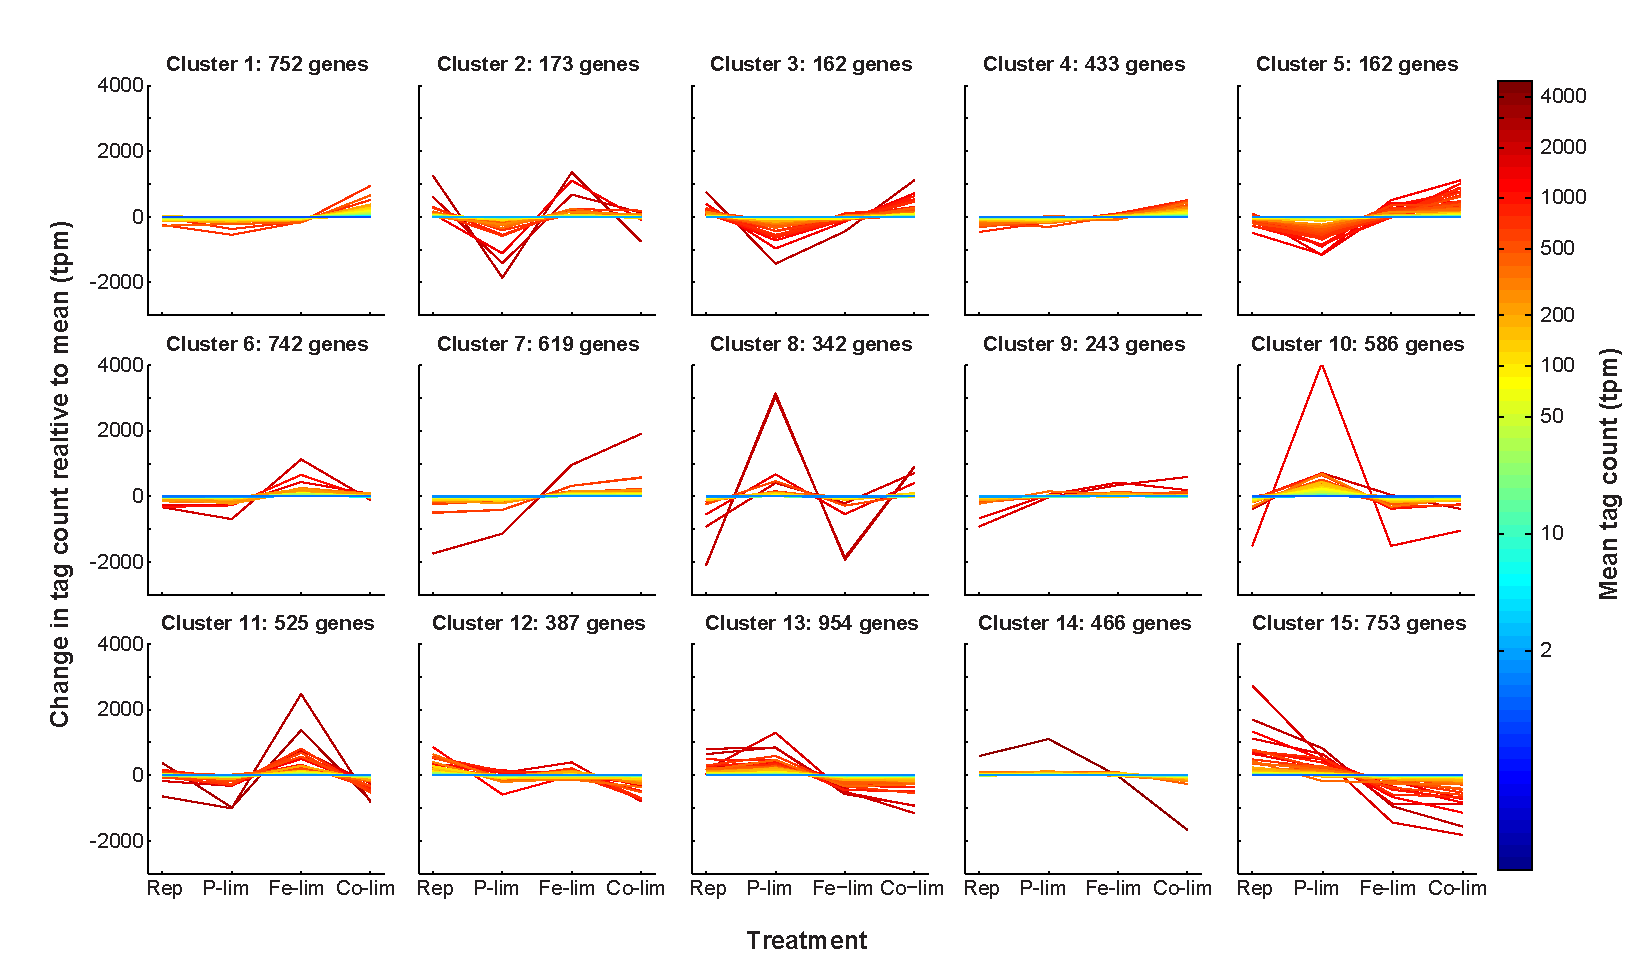
\includegraphics[width=1\textwidth]{Images/C2_FigureS2_v6.pdf}
        \caption[$K$-means clustering of normalized genes]{$K$-means clustering of normalized genes. The 7380 genes that passed the 2.5 TPM cutoff were clustered into 15 clusters using the $k$-means algorithm under the Pearson correlation coefficient. Tag counts normalized to total library size (in TPM) for each gene are plotted relative to the mean (indicated by the color of the line) for each of the four treatments: Replete (Rep), P-limited (P-lim), Fe-limited (Fe-lim), and co-limited (Co-lim).}
    \label{fig:a1f2} 
    \end{figure}
    \vfill        %%<----- and here
\end{landscape}

\clearpage
\newpage

%%%%%%%%%%%%%%%%%%%%%%%%%%%

%%%%%%%%%%%%%%%%%%%%%%%%%%%_________________CHAPTERTHREE_________________%%%%%%%%%%%%%%%%%%%%%%%%%%%

%%%%%%%%%%%%%%%%%%%%%%%%%%%


\section{Appendix for Chapter 3}
\subsection{Supplemental Figures}

%Supplemental Figure 1: Cell counts in NB 
\begin{figure}[h!]
  \centering
    \includegraphics[width=1\textwidth]{Images/C3_SFigure1_CellCounts.png}
    \caption[Cell counts in Narragansett Bay during the spring of 2012]{Abundance estimation from cell counts of \textit{Skeletonema} spp. and \textit{T. rotula} across the five sample points during the spring of 2012. }
  \label{fig:a3f1}
\end{figure}


%Supplemental Figure 2: KEGG linear correlation
\begin{figure}[p!]
  \centering
    \includegraphics[width=1\textwidth]{Images/C3_SFigure2_KEGGModuleGeneContent2.png}
    \caption[Comparison of KEGG module content between \textit{Skeletonema} spp. and \textit{T. rotula} ]{Total number of genes assigned to each KEGG module for \textit{Skeletonema} spp. and \textit{T. rotula}.}
  \label{fig:a3f2}
\end{figure}


%Supplemental Figure 3: Hierarchical clustering of S and T across time
\begin{figure}[p!]
  \centering
    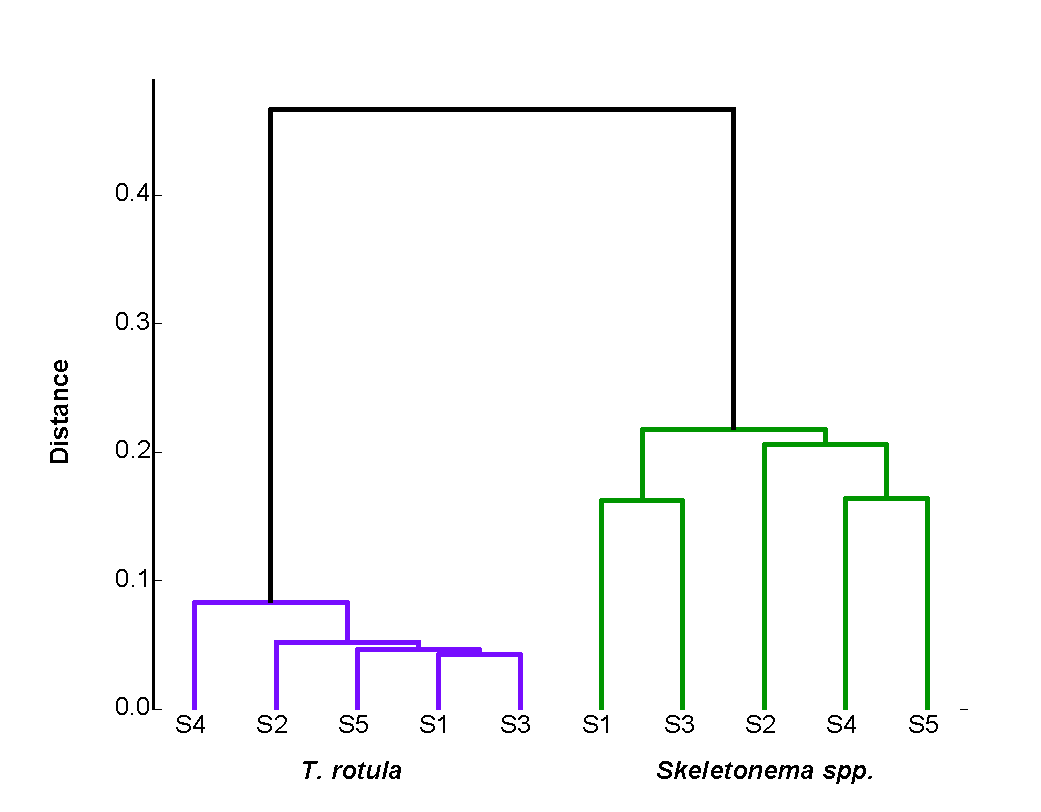
\includegraphics[width=1\textwidth]{Images/C3_SFigure3_Dendrogram.pdf}
    \caption[Hierarchical clustering of QMF signatures across species and samples]{Dendrogram depicting hierarchical clustering of samples based on relative expression of KEGG modules (Figure 2) across the five samples S1-S5 for \textit{Skeletonema} spp. and \textit{T. rotula}.}
  \label{fig:a3f3}
\end{figure}

%Supplemental Figure 4: Stable gene expression across time
\begin{figure}[p!]
  \centering
    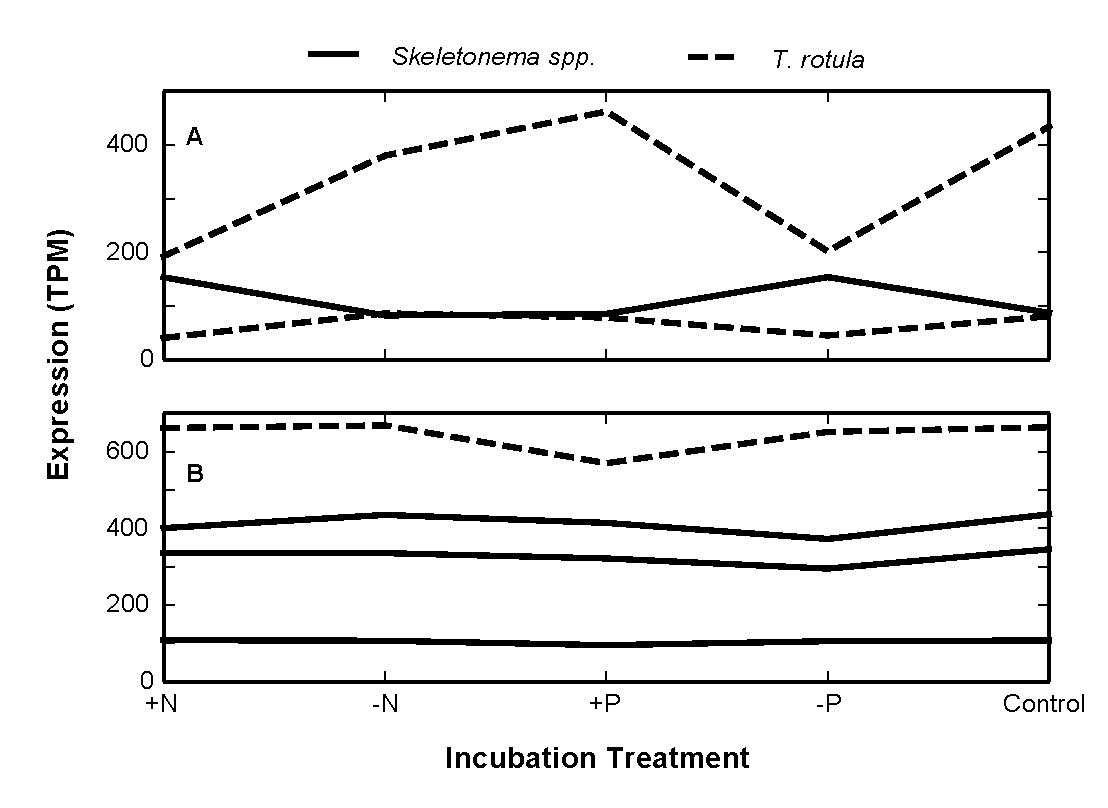
\includegraphics[width=1\textwidth]{Images/C3_SFigure4_StableGenePlot_wActin.pdf}
    \caption[Expression of stable reference genes in the field]{Expression of stable reference genes identified based on literature and statistical parsing in nutrient amendment incubation. (A) The expression in tags per million ($TPM$) of stable reference genes identified in \textit{T. rotula} (dashed line) and \textit{Skeletonema} spp.  (solid lines) based on homology (e-value < 1e-5) to a known reference genes in \textit{T. pseudonana}, ACT1 (Thaps\_25772), in nutrient incubations. (B) Also shown are reference genes identified in the incubation experiments, using statistical analysis of sequence counts \citep{Alexander2012, Wu2010}, and nutrient incubations }
  \label{fig:a3f4}
\end{figure}

%Supplemental Figure 5: RR gene composition
\begin{figure}[p!]
  \centering
    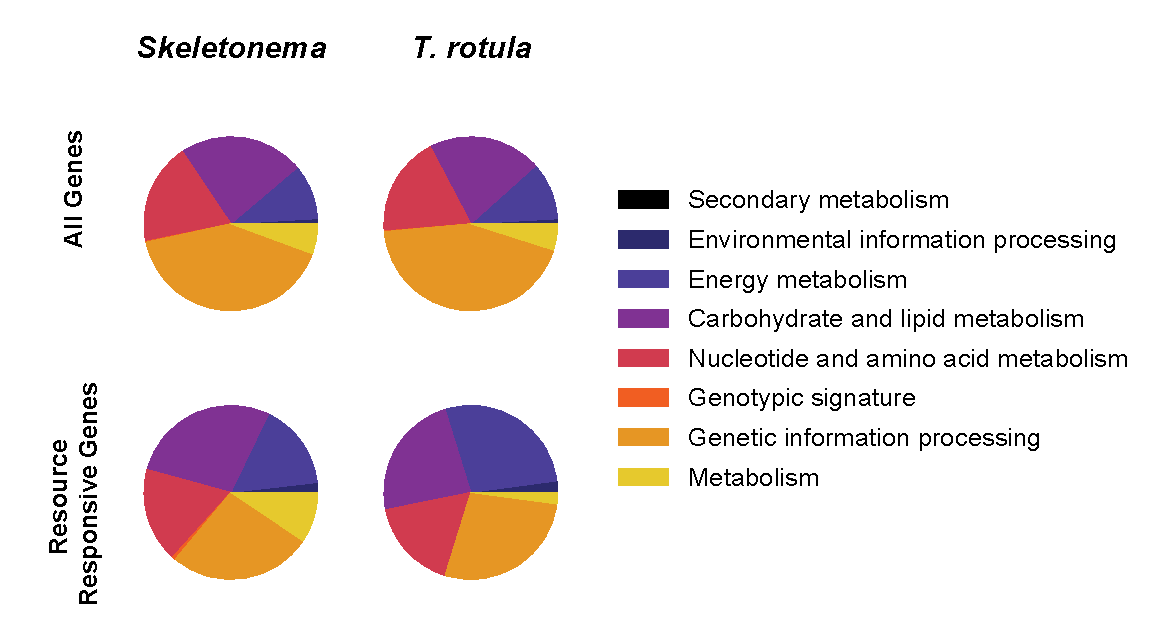
\includegraphics[width=1\textwidth]{Images/C3_SFigure5_RR_All_Genes_Pie.pdf}
    \caption[Functional compoosition of the reference transcriptome and resource-responsive gene sets]{Functional composition of the reference transcriptome and resource-responsive (RR) gene subset for \textit{T. rotula} and \textit{Skeletonema} spp. (A) RR gene sets were identified through cross comparison of like-nutrient incubations (i.e. +N vs. -N and +P vs. -P), using ASC (fold change = 2, post-$p > 0.95$). The relative functional categorization of the reference transcriptomes and RR gene set for \textit{T. rotula} and \textit{Skeletonema} spp. based on KEGG ontology as assigned by KAAS is depicted at the module-level.}
  \label{fig:a3f5}
\end{figure}

%Supplemental Figure 6: Expression of nitrate reductase

\begin{figure}[p!]
  \centering
    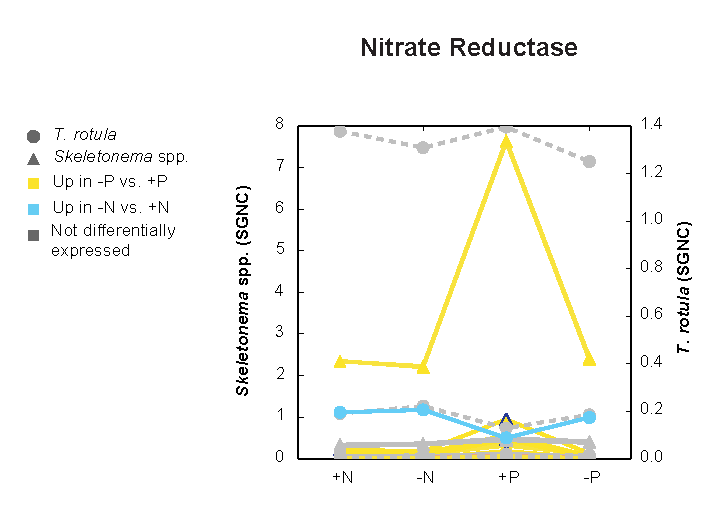
\includegraphics[width=1\textwidth]{Images/C3_SFigure6_SGNC_NitrateReductase.pdf}
    \caption[Relative expression of nitrate reducatses across incubation experiments]{The relative expression in stable gene normalized counts ($SGNC$) of the assimilatory nitrate reductase gene cluster across the incubation experiment treatments. Significance of regulation between the treatments is denoted by the color of the line; organisms are denoted by the shapes of the marker.}
  \label{fig:a3f6}
\end{figure}

%Supplemental Figure 7: Cluster Analysis


\begin{figure}[p!]
  \centering
    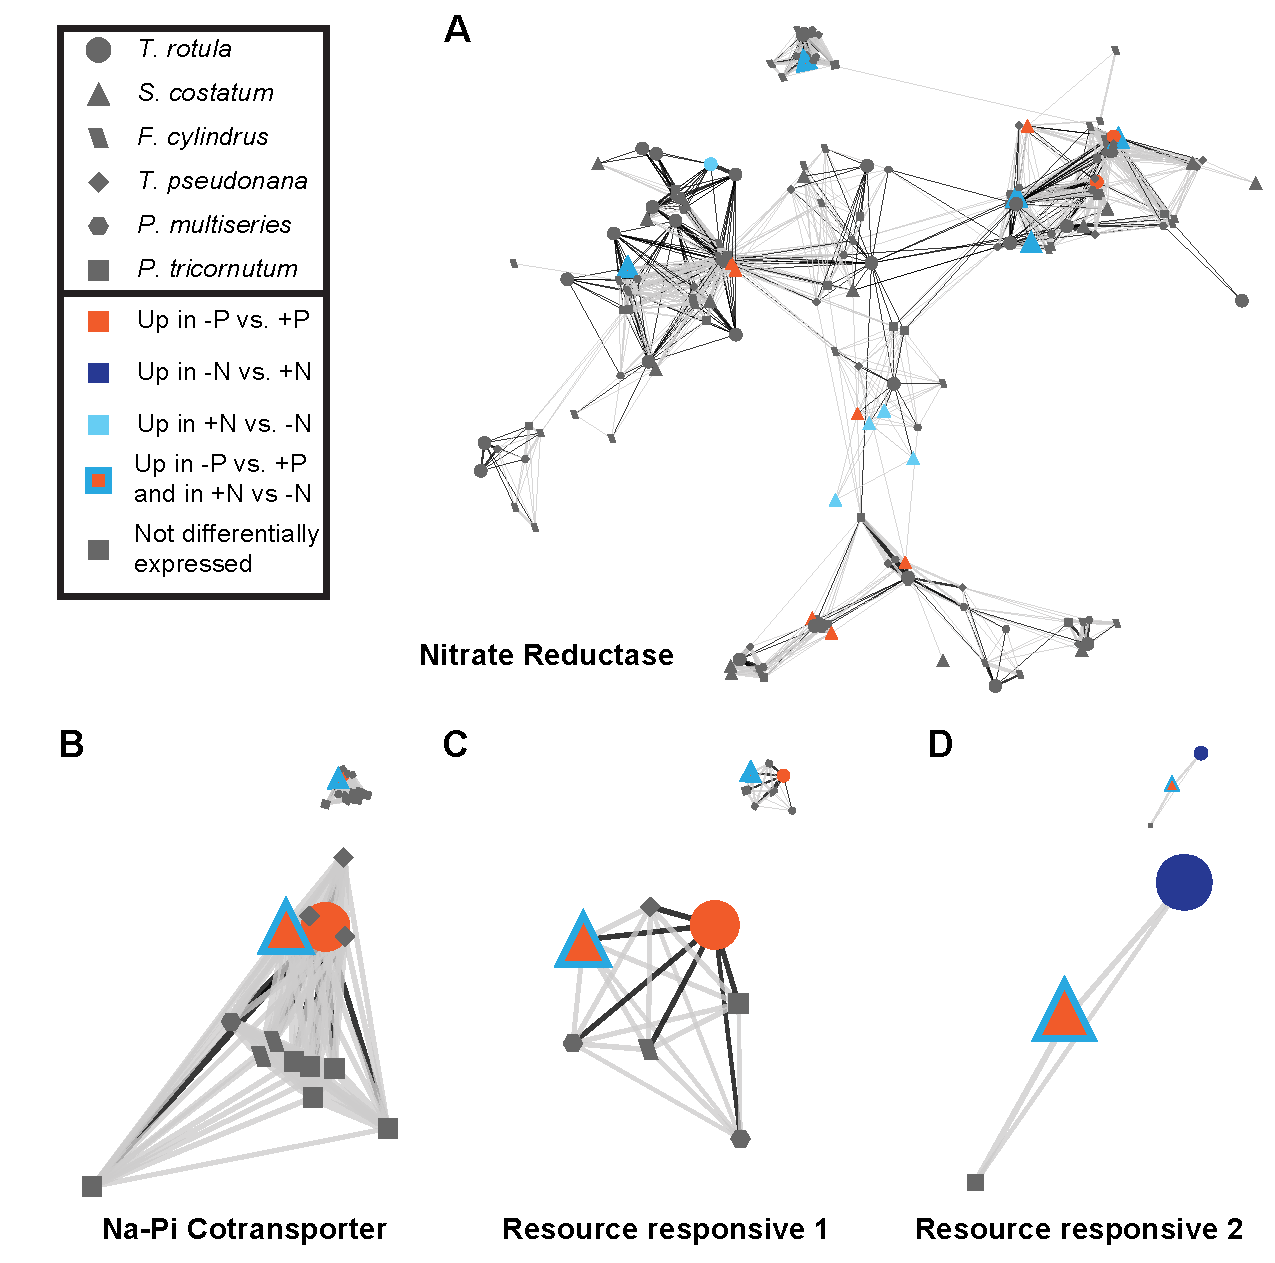
\includegraphics[width=1\textwidth]{Images/C3_SFigure7_ClusterAnalysis_v5.pdf}
    \caption[Gene cluster analysis of nutrient-responsive genes]{Gene cluster known nutrient-responsive genes in \textit{T. pseudonana}: (A) assimilatory nitrate reductase and (B) sodium-phosphate cotransporter and novel resource-responsive (RR) gene families: (C) RR1 and (D) RR2. Transcripts from the transcriptomes of \textit{T. rotula} and \textit{Skeletonema} spp. were clustered based upon relative homology with available diatom genomes: \textit{F. cylindrus}, \textit{P. tricornitum}, \textit{P. multiseries}, and \textit{T. pseudonana}. Symbols indicate different species, while color indicates regulation in the field incubation experiments. Two nodes within a gene cluster are connected by an edge if they share a homologous protein (reciprocal BLAST hit with a minimum of 1e-5 score and minimum 20\% identity). Gene clusters are visualized using an edge-weighted spring-embedded model based on e-value, meaning that genes that are closer together are more similar. The width of the line correlates to the magnitude of the e-value, with lower e-values represented by thicker lines and higher e-values represented by thinner lines.}
  \label{fig:a3f7}
\end{figure}

%Supplemental Figure 8: Conceptual schematic of STD niche space

\begin{figure}[p!]
  \centering
    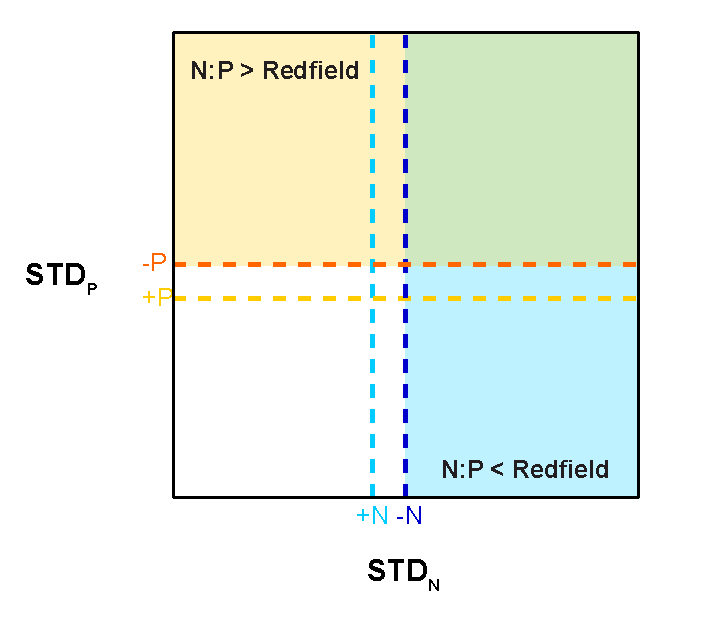
\includegraphics[width=1\textwidth]{Images/C3_SFigure8_Schematic_Quadrants.pdf}
    \caption[Conceptual schemiatic of $STD_N$ plotted against $STD_P$]{A conceptual schematic of $STD_N$ plotted against $STD_P$ hypothesized regions of N:P > Redfield physiology and N:P < Redfield physiology highlighted.}
  \label{fig:a3f8}
\end{figure}


%Supplemental Figure 9: NISP Dn genes
\begin{landscape}
   \centering
   \null         %%<---- this is needed
   \vfill        %%<-----here

	\begin{figure}
  	\centering
    	\includegraphics[width=1.3\textwidth]{Images/C3_SFigure9_NISP_DNGenes.png}
    	\caption[Evolution of niche space indexing over for significantly down-regualted genes]{Evolution of niche space indexing over time in Narragansett Bay for \textit{T. rotula} and \textit{Skeletonema} spp.. The stable gene normalized field signal from genes identified as significantly (2-fold change, post$-p > 0.95$) down-regulated in -P vs +P for Skeletonema spp. (yellow) and \textit{T. rotula} (orange) and in -N vs +N for for \textit{Skeletonema} spp. (cyan) and \textit{T. rotula} (dark blue) was proportionalized relative to the expression for those genes in nutrient incubations, yielding the $STD_N$ and $STD_P$. These data are plotted for Sample 1 through Sample 5.}
  	\label{fig:a3f9}
	\end{figure}
    \vfill        %%<----- and here
\end{landscape}

%Supplemental Figure 10: Percentage of RR genes by quadrant

\begin{figure}[h!]
  \centering
    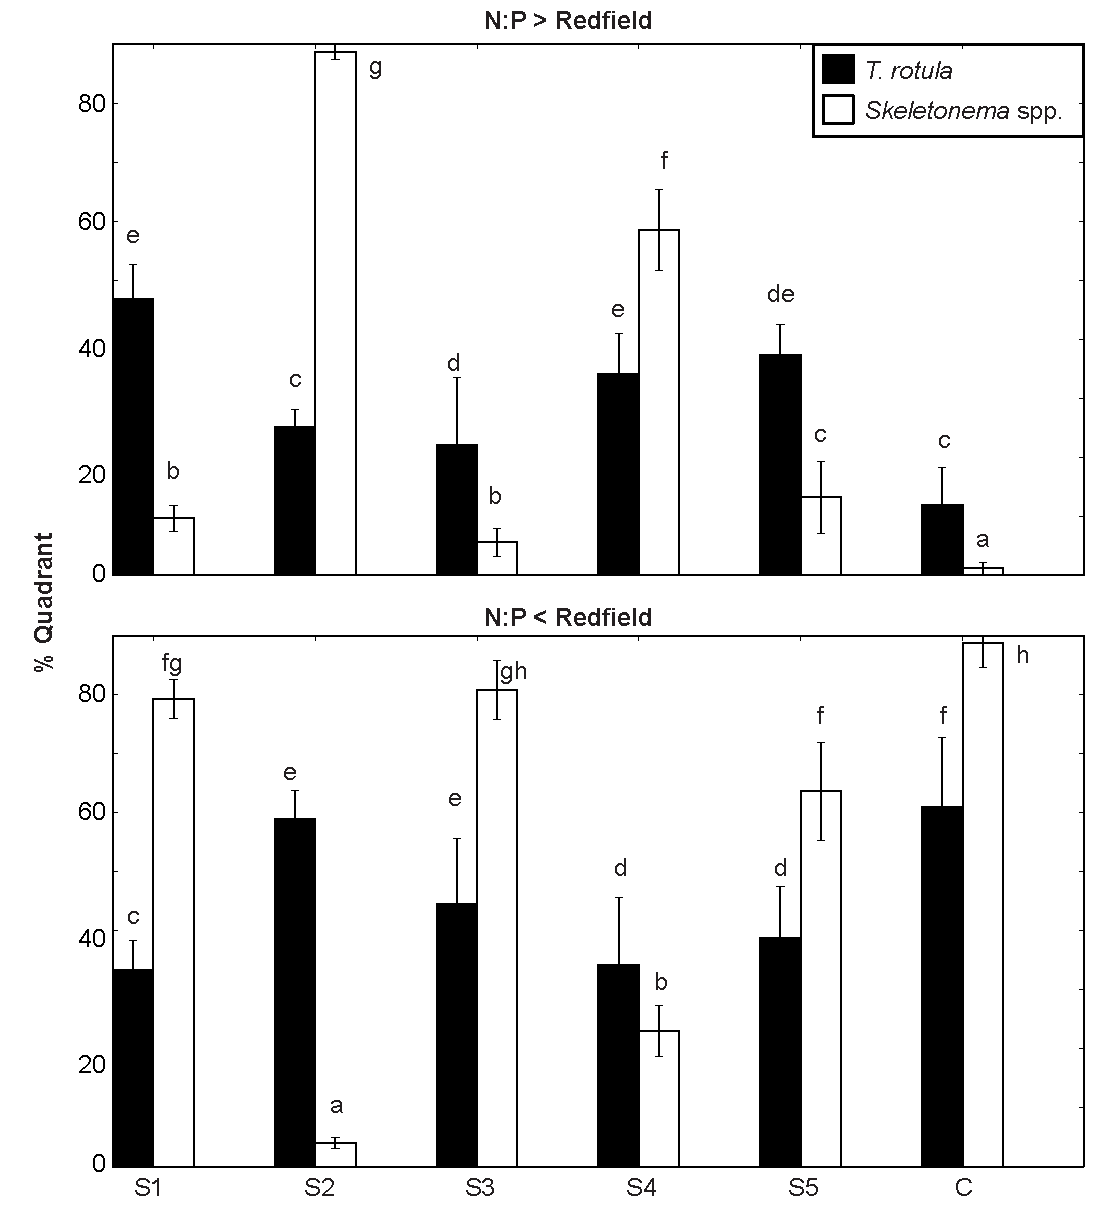
\includegraphics[width=1\textwidth]{Images/C3_SFigure10_BarGraph_Quadrant_2575_stats.pdf}
    \caption[The percentage of identified nutrient responsive genes falling into the N:P > Redfield and N:P < Redfield quadrants with varried cutoffs]{The percentage of identified nutrient responsive genes falling into the N:P > Redfield and N:P < Redfield quadrants for \textit{T. rotula} and \textit{Skeletonema} spp.. The total number of genes falling into the N:P > Redfield quadrant ($STD_P > C$; $STD_N < C$, for $0.25 < C < 0.75$) and the N:P < Redfield quadrant ($STD_P$ < C; $STD_N > C$, for $0.25 < C < 0.75$). The value of C was varied over 10 different values and the average percentages of genes falling into each of the quadrants is depicted above based on the size of the circle at the median $STD_N$ and $STD_P$ for the genes in the quadrant. Similarity of data between species by quadrant was assessed using an analysis of variance (ANOVA) with a generalized linear model. The results from a post hoc Tukey test show the divergence of species across time ($p < 0.05$).}
  \label{fig:a3f10}
\end{figure}

%Supplemental Figure 11: Quadrant localization with varying stable reference genes

\begin{figure}[p!]
  \centering
    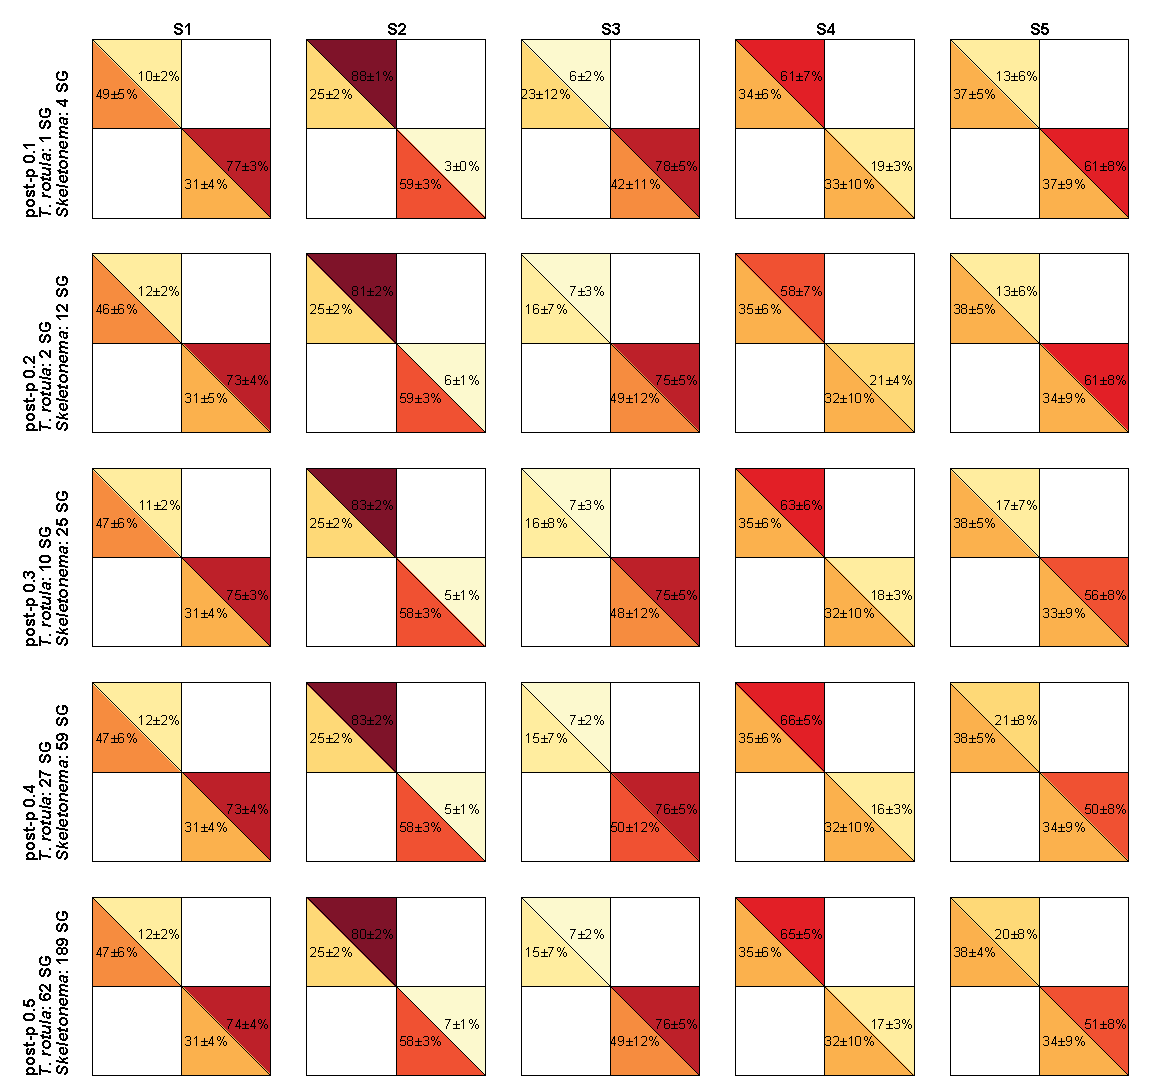
\includegraphics[width=1\textwidth]{Images/C3_SFigure11_Quadrant.pdf}
    \caption[The impact of stable gene selction of quadrant localization]{The impact of stable gene selection on the quadrant localization of the resource responsive gene sets. The posterior probability cutoff used in the selection of stable genes was varied from 0.1 to 0.5 for a fold change of 1.25. The percentage of identified nutrient responsive genes falling into the N:P > Redfield and N:P < Redfield quadrants for \textit{T. rotula} and \textit{Skeletonema} spp. across the five sample points and five posterior probability values is depicted.}
  \label{fig:a3f11}
\end{figure}



\subsection{Supplemental Tables}

%Supplemental Table 1: library stats

\begin{table}[h!]
\centering
\caption[The total number of paired end reads after quality control and trimming and the percentage of reads mapping]{The total number of paired end reads after quality control and trimming and the percentage of reads mapping to the \textit{T. pseudonana} genome, \textit{T. rotula} transcriptome, and \textit{S. costatum} transcriptome.}
\label{tab:a3t1}

\newcolumntype{C}[1]{>{\centering\let\newline\\\arraybackslash\hspace{.5pt}}m{#1}}

\begin{tabular}{|C{2cm}|C{2.5cm}|C{2.5cm}|C{2.5cm}|C{2.5cm}|}
\hline
\multirow{2}{*}{Sample} & \multirow{2}{*}{\parbox{2.5cm}{Total library size (paired end reads)}} & \multicolumn{3}{c|}{Mapped representation in library} \\ \cline{3-5} 
                        &                                                              & \textit{T. pseudonana}      & \textit{T. rotula}      & \textit{S. costatum}     \\ \hline
S1                      & 89455034                                                     & 2.98\%             & 17.50\%        & 33.50\%         \\ \hline
S2                      & 64888267                                                     & 0.41\%             & 11.70\%        & 54.90\%         \\ \hline
S3                      & 103250243                                                    & 0.39\%             & 7.30\%         & 9.00\%          \\ \hline
S4                      & 45370867                                                     & 0.68\%             & 8.80\%         & 8.30\%          \\ \hline
S5                      & 55061692                                                     & 0.88\%             & 10.40\%        & 11.20\%         \\ \hline
Ambient Control         & 51508197                                                     & 0.27\%             & 13.40\%        & 8.00\%          \\ \hline
+N                      & 58626239                                                     & 0.43\%             & 6.10\%         & 5.30\%          \\ \hline
-N                      & 44561851                                                     & 0.41\%             & 8.70\%         & 8.30\%          \\ \hline
+P                      & 51130364                                                     & 0.29\%             & 8.50\%         & 8.00\%          \\ \hline
-P                      & 58834022                                                     & 0.40\%             & 6.60\%         & 6.50\%          \\ \hline
\end{tabular}
\end{table}

%Supplememntal Table 2: nutrient concentrations used in incubations

\begin{table}[h!]
\centering
\caption[Nutrient concentrations used in nutrient amendment incubations. ]{Nutrient concentrations used in nutrient amendment incubations.}
\label{tab:a3t2}
\begin{tabular}{|c|c|c|c|c|c|}
\hline
                                    & \multicolumn{5}{c|}{\textbf{Treatment}}                                                                                              \\ \cline{2-6} 
\multirow{-2}{*}{\textbf{Nutrient}} & Ambient Control          & + P                      & + N                      & - P                      & - N                      \\ \hline
Nitrate                             & \cellcolor[HTML]{C0C0C0} & \cellcolor[HTML]{C0C0C0} & 10 $\mu M$                    & 10 $\mu M$                    & \cellcolor[HTML]{C0C0C0} \\ \hline
Phosphate                           & \cellcolor[HTML]{C0C0C0} & 3 $\mu M$                     & \cellcolor[HTML]{C0C0C0} & \cellcolor[HTML]{C0C0C0} & 3 $\mu M$                     \\ \hline
Silica                             & \cellcolor[HTML]{C0C0C0} & \cellcolor[HTML]{C0C0C0} & \cellcolor[HTML]{C0C0C0} & 68 $\mu M$                    & 68 $\mu M$                    \\ \hline
Iron                                & \cellcolor[HTML]{C0C0C0} & \cellcolor[HTML]{C0C0C0} & \cellcolor[HTML]{C0C0C0} & 4.6 $\mu M$                   & 4.6 $\mu M$                   \\ \hline
Vitamins                            & \cellcolor[HTML]{C0C0C0} & \cellcolor[HTML]{C0C0C0} & \cellcolor[HTML]{C0C0C0} & f/5                      & f/5                      \\ \hline
\end{tabular}
\end{table}


%Supplememntal Table 3: nutrient concentrations used in incubations

\begin{table}[h!]
\centering
\caption[Mapping statistics for \textit{T. rotula} and \textit{S. costatum} transcriptomes]{Total number of contigs in the \textit{T. rotula} and \textit{S. costatum} transcriptomes and the number of genes in each of the differentially regulated and stable groupings.}
\label{tab:a3t3}
\begin{tabular}{|l|l|l|}
\hline
                                                                       & \textit{\textbf{T. rotula}} & \textit{\textbf{S. costatum}} \\ \hline
Number of contigs in transcriptome                                     & 22362                       & 27665                         \\ \hline
Pass 2 TPM cutoff                                                      & 4318                        & 20921                         \\ \hline
Up in -P vs +P                                                         & 249                         & 4754                          \\ \hline
Down in -P vs +P                                                       & 335                         & 52                            \\ \hline
Up in -N vs +N                                                         & 196                         & 9                             \\ \hline
Down in -N vs +N                                                       & 49                          & 1631                          \\ \hline
All differentially regulated (2 fold change, post-$p > 0.95$) & 775                         & 5136                          \\ \hline
Stable genes (1.25 fold change, post-$p < 0.1$)                  & 1                           & 4                             \\ \hline
\end{tabular}
\end{table}




%%%%%%%%%%%%%%%%%%%%%%%%%%%

%%%%%%%%%%%%%%%%%%%%%%%%%%%_________________CHAPTERFOUR_________________%%%%%%%%%%%%%%%%%%%%%%%%%%%

%%%%%%%%%%%%%%%%%%%%%%%%%%%


\clearpage

\section{Appendix for Chapter 4}
\subsection{Supplemental Figures}

%Supplemental Figure 1: Chlorophyll values in experiments and in situ samples 
\begin{figure}[h!]
  \centering
    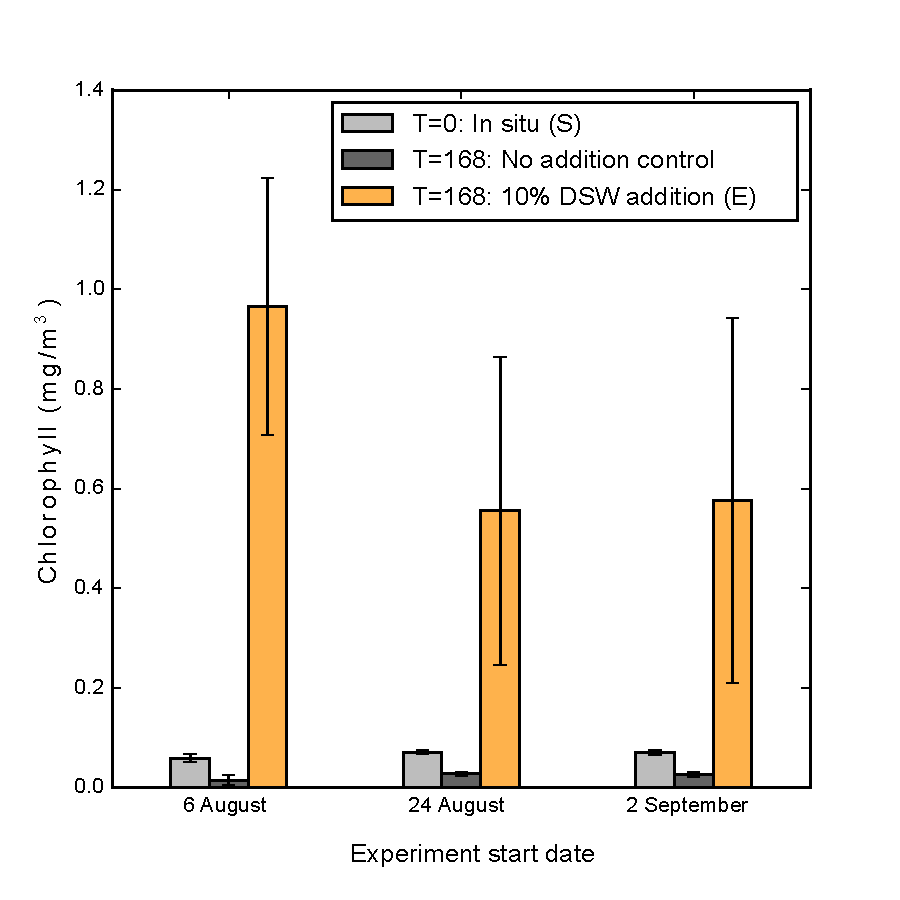
\includegraphics[width=1\textwidth]{Images/C4_FigureS1.pdf}
    \caption[Chlorophyll a of replicated experiments for \emph{in situ} samples, no addition control, and a 10\% deep seawater amendment]{Chlorophyll a of replicated experiments for \emph{in situ} samples (S), a no addition control, and a 10\% deep seawater (DSW) amendment (E). Incubation samples were harvested after 168 hours.}
  \label{fig:a4f1}
\end{figure}


%Supplemental Figure 2: Rank abundance shifts in species composition of diatoms, haptophytes and dinoflagellates

\begin{figure}[p!]
  \centering
    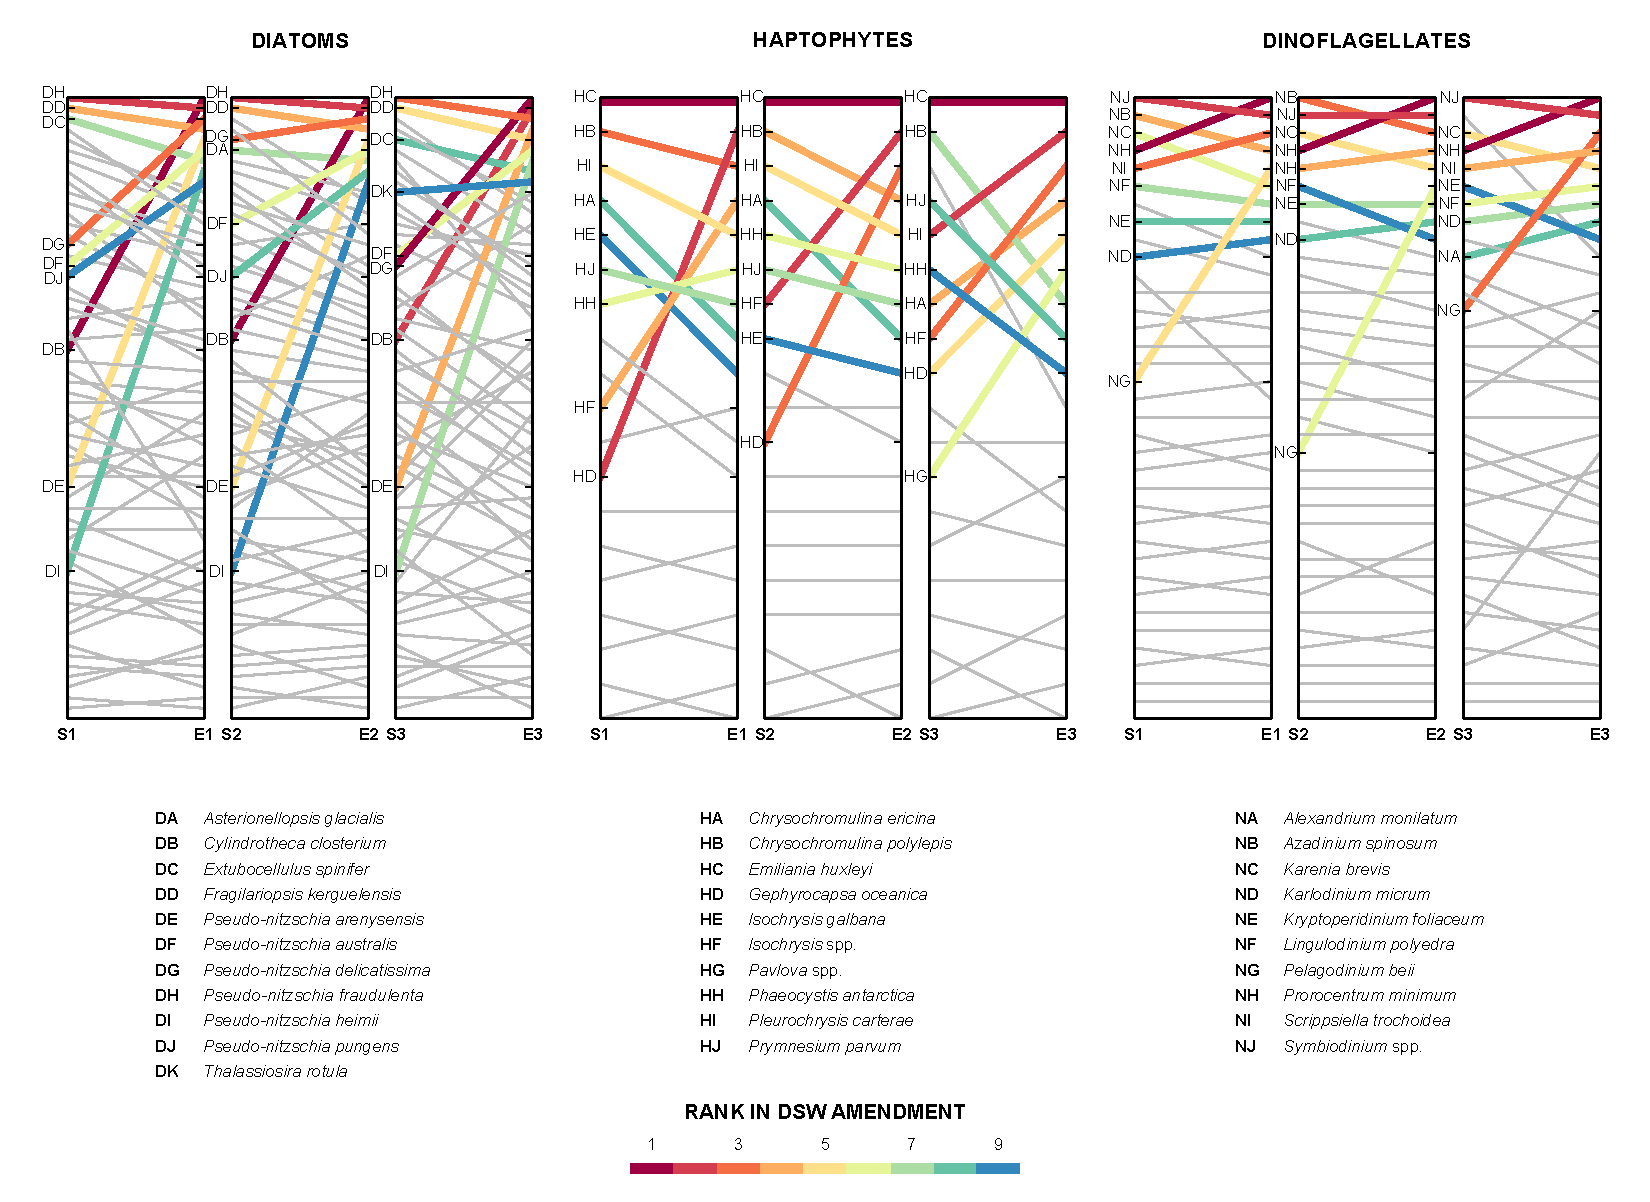
\includegraphics[width=1\textwidth]{Images/C4_FigureS2.pdf}
    \caption[Rank abundance shifts in the species composition of diatoms, haptophytes and dinoflagellates]{Rank abundance shifts in the species composition of diatoms, haptophytes and dinoflagellates for the three experiments. The relative shift in rank abundance for each species is depicted for each incubation experiment (E1-E3) following deep seawater (DSW) addition. The nine most abundant taxa following DSW addition are highlighted for each of the functional groups. Although the species that recruited the reads are denoted here this is highly driven by the composition of the database and does not necessarily indicate the actual species present, but rather the closest species present in the database.}
  \label{fig:a4f2}
\end{figure}

%Supplemental Figure 3: QMF Comparison across species


\begin{figure}[p!]
  \centering
    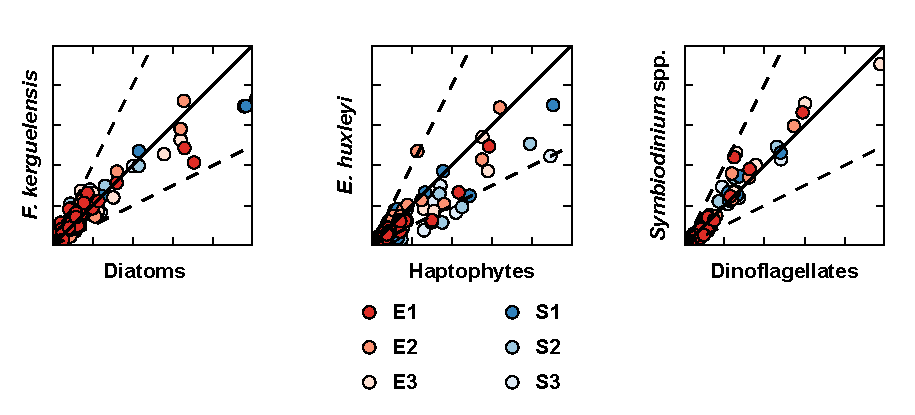
\includegraphics[width=1\textwidth]{Images/C4_FigureS3.pdf}
    \caption[Comparison of the quantitative metabolic fingerprint (QMF) between the whole functional group and representative taxa]{Comparison of the quantitative metabolic fingerprint (QMF) between the whole functional group and representative taxa. The proportion of reads falling into each of the modules depicted in Figure 2 is plotted for S1-S3 and E1-E3, comparing the summed functional group signal and that of a representative taxon. Color of the marker indicates the sample; solid and dashed lines mark the 1:1 and 1:2 lines, respectively.}
  \label{fig:a4f3}
\end{figure}

%Supplemental Figure 4: Distribution histogram

\begin{figure}[p!]
  \centering
    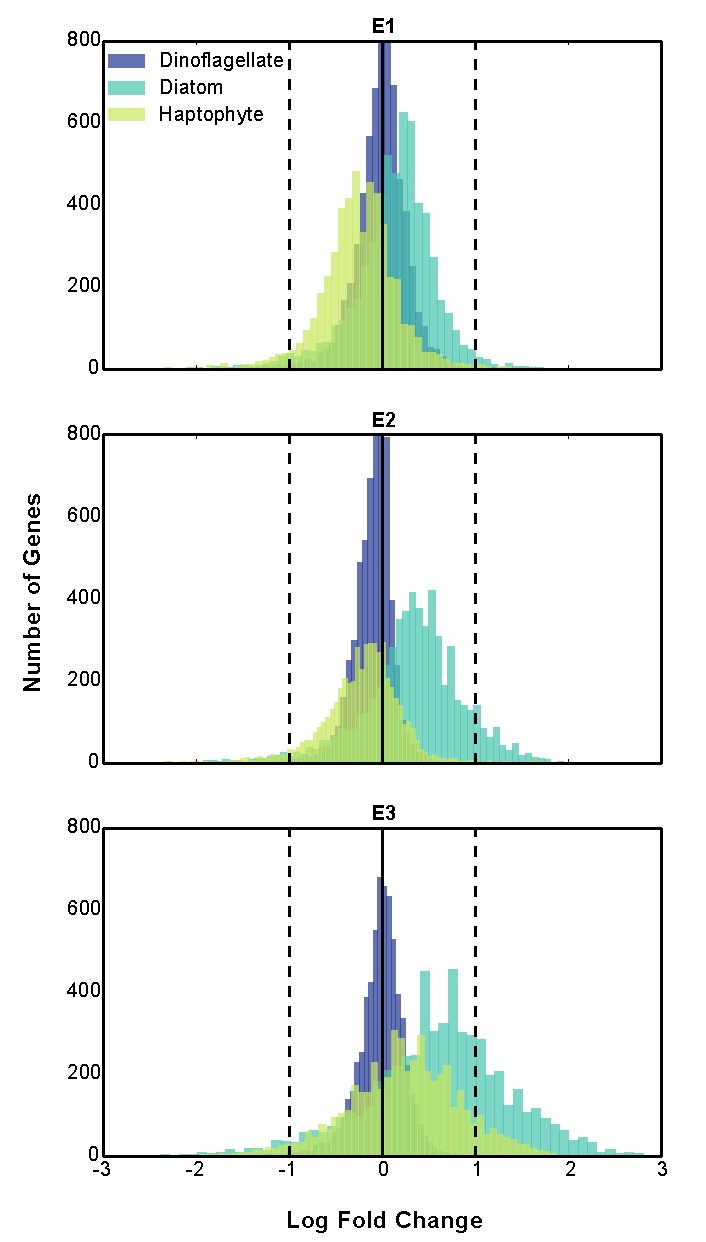
\includegraphics[width=.75\textwidth]{Images/C4_FigureS4.png}
    \caption[Distribution of log fold change following deep seawater (DSW) addition]{Distribution of log fold change following deep seawater (DSW) addition. Histogram of the number of genes falling within each of the log fold change bins for diatoms, haptophytes and dinoflagellates. Solid line indicates no fold change; dashed lines indicate 2 fold-change both up and down.}
  \label{fig:a4f4}
\end{figure}


%Supplemental Figure 5: Weight venn diagrams for up and down regulated genes

\begin{figure}[p!]
  \centering
    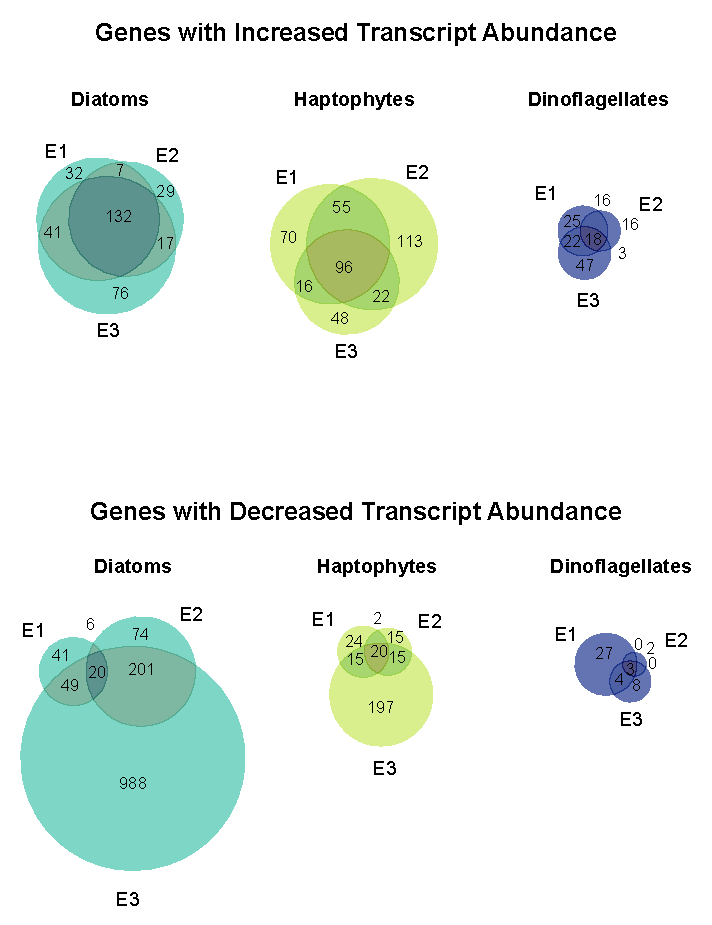
\includegraphics[width=1\textwidth]{Images/C4_FigureS5.pdf}
    \caption[Weighted Venn diagrams of genes with significantly different abundances following deep seawater (DSW) addition by functional group]{Weighted Venn diagrams of genes with significantly different abundances following deep seawater (DSW) addition by functional group. The uniqueness of KEGG orthologs with increased or decreased abundances as determined by ASC (2 fold-change, post-p > 0.95) across experiments was assessed for diatoms, haptophytes, and dinoflagellates.}
  \label{fig:a4f5}
\end{figure}


%Supplemental Figure 6: MANTA Plots

\begin{figure}[p!]
  \centering
    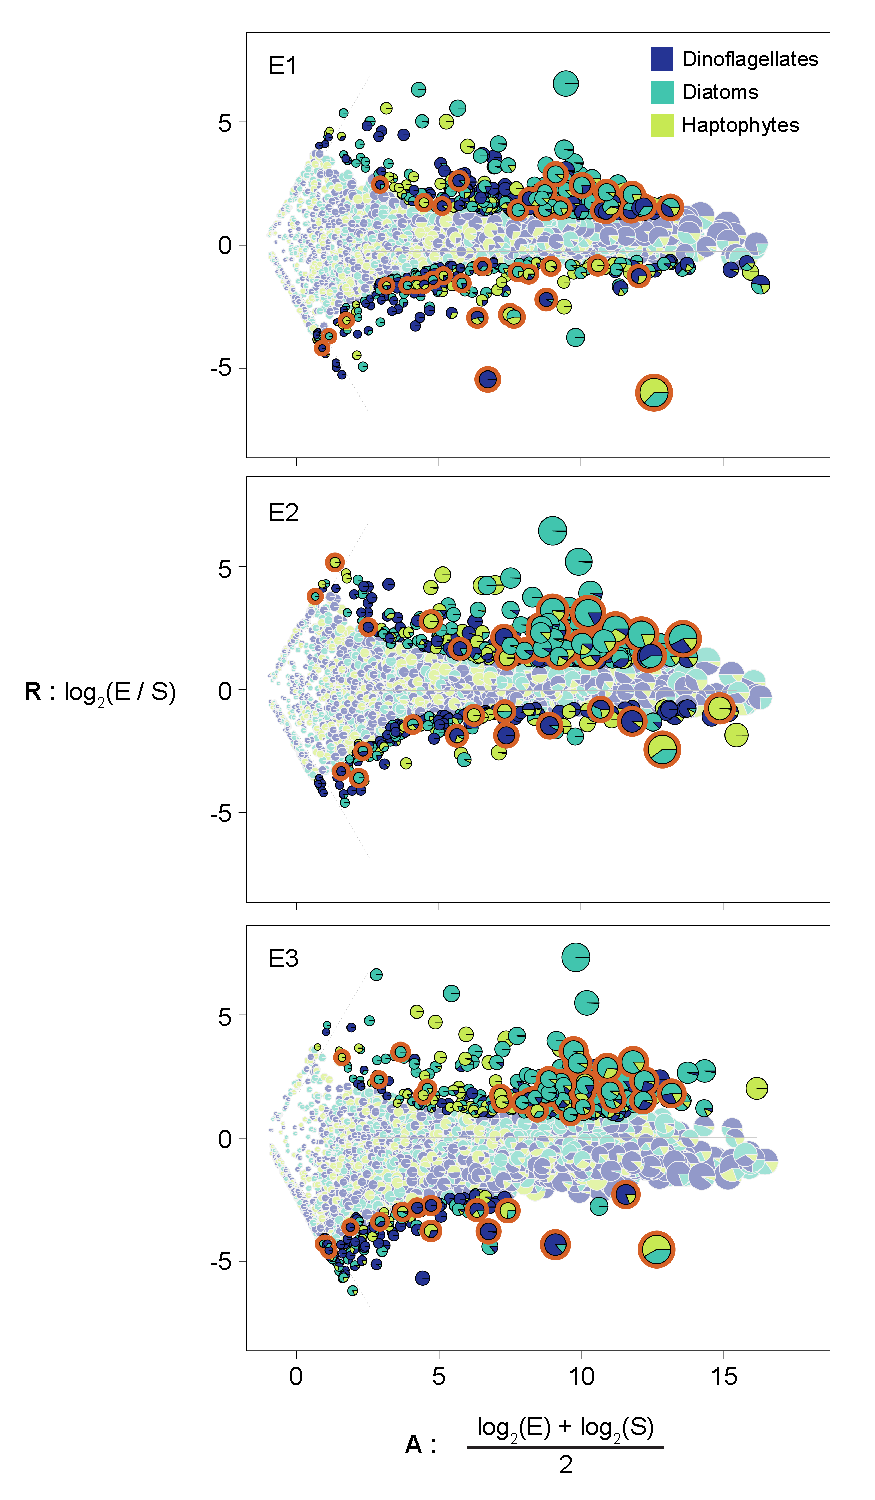
\includegraphics[width=.7\textwidth]{Images/C4_FigureS6.pdf}
    \caption[Microbial Assemblage Normalized Transcript Analysis (MANTA) ratio-averaged plots for global shifts in expression of KEGG orthologs]{Microbial Assemblage Normalized Transcript Analysis (MANTA) ratio-averaged plots for global shifts in expression of KEGG orthologs. Fold change ratio (R) and average read count (A) are plotted for read counts in the \emph{in situ} (S) and deep seawater (DSW) amendment (E) samples across the three sample pairs (S1:E1, S2:E2, S3:E3). The trimmed mean of fold-change values is noted as a gray solid line; orthologs unique to one library are separated by gray dashed lines. Pies indicate the taxonomic distribution of orthologous reads across the three functional groups. KEGG orthologs that were significantly differentially expressed (DE) (adjusted $P > 0.05$) are outlined in black and those not significantly DE are outlined in gray. DE KEGG orthologs that fall in the Energy Metabolism KEGG module are outlined in orange.}
  \label{fig:a4f6}
\end{figure}

%Supplemental Figure 7: QMF across incubation experiments

\begin{figure}[p!]
  \centering
    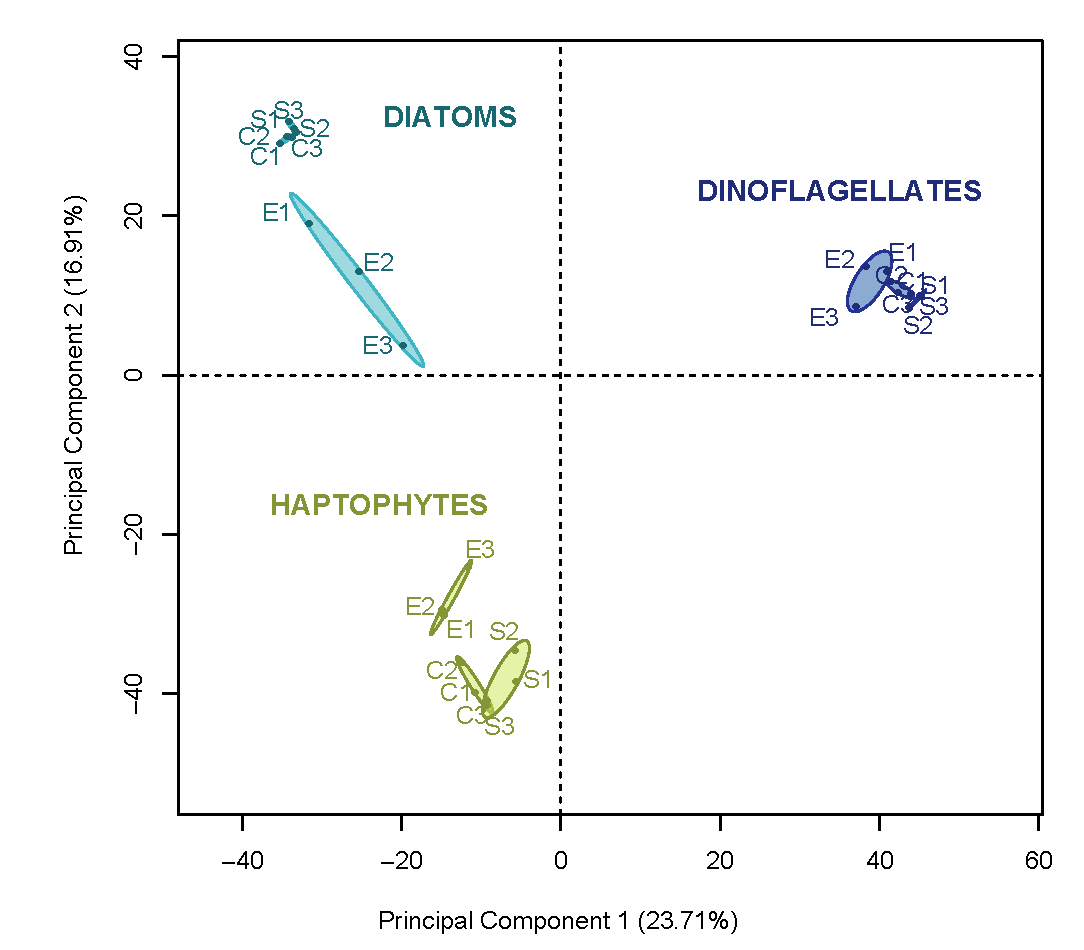
\includegraphics[width=1\textwidth]{Images/C4_FigureS7.pdf}
    \caption[Principal component analysis of the quantitative metabolic fingerprint (QMF) signals across \emph{in situ}, no addition control, and deep seawater amended samples]{Principal component analysis of the quantitative metabolic fingerprint (QMF) signals across \emph{in situ}, no addition control, and deep seawater (DSW) amended samples. Principal component analysis of the QMF signals for each of the functional groups across \emph{in situ} (S1-S3), control no addition (C1-C3) and DSW amendment (E1-E3); 95\% confidence ellipses are indicated for each of the sample types by functional group.}
  \label{fig:a4f7}
\end{figure}

\clearpage

\subsection{Supplemental Tables}

% Supplemental table with nutrient concentrations post treatment run for E and C
\begin{table}[h!]
\centering
\caption[Mapping statistics for \textit{T. rotula} and \textit{S. costatum} transcriptomes]{Total number of contigs in the \textit{T. rotula} and \textit{S. costatum} transcriptomes and the number of genes in each of the differentially regulated and stable groupings.}
\label{tab:a4t1}
\newcolumntype{C}[1]{>{\centering\let\newline\\\arraybackslash\hspace{.5pt}}m{#1}}
\begin{tabular}{ccccc}

    
\hline
\multicolumn{1}{|c|}{\multirow{2}{*}{\textbf{Treatment}}} & \multicolumn{1}{c|}{\multirow{2}{*}{\textbf{\begin{tabular}[c]{@{}c@{}}Time post \\ inoculation (hours)\end{tabular}}}} & \multicolumn{1}{c|}{\multirow{2}{*}{\textbf{\begin{tabular}[c]{@{}c@{}}NO2 + NO3 \\ ($\mu M$)\end{tabular}}}} & \multicolumn{1}{c|}{\multirow{2}{*}{\textbf{\begin{tabular}[c]{@{}c@{}}PO4 \\ ($\mu M$)\end{tabular}}}} & \multicolumn{1}{c|}{\multirow{2}{*}{\textbf{\begin{tabular}[c]{@{}c@{}}Si\\ ($\mu M$)\end{tabular}}}} \\

\multicolumn{1}{|c|}{}                                    & \multicolumn{1}{c|}{}                                                        & \multicolumn{1}{c|}{}                                                                                    & \multicolumn{1}{c|}{}                                                                              & \multicolumn{1}{c|}{}                                                                            \\ \hline
\multicolumn{1}{|c|}{\textbf{C} (control no addition) *}  & \multicolumn{1}{c|}{168}                                                     & \multicolumn{1}{c|}{$0.12 \pm 0.03$}                                                                         & \multicolumn{1}{c|}{$0.12 \pm 0.02$}                                                                   & \multicolumn{1}{c|}{$1.91 \pm 0.2$}                                                                  \\ \hline
\multicolumn{1}{|c|}{\textbf{E} (+ 10\% DSW) *}           & \multicolumn{1}{c|}{168}                                                     & \multicolumn{1}{c|}{$1.9 \pm  .93$}                                                                          & \multicolumn{1}{c|}{$0.23 \pm 0.05$}                                                                   & \multicolumn{1}{c|}{$8.46 \pm 3.11$}                                                                 \\ \hline
\multicolumn{1}{|c|}{\textbf{DSW} (700 m water) *}        & \multicolumn{1}{c|}{N/A}                                                     & \multicolumn{1}{c|}{$37.5 \pm 1.68$}                                                                         & \multicolumn{1}{c|}{$3.14 \pm 0.03$}                                                                   & \multicolumn{1}{c|}{$83.4 \pm 9.33$}                                                                 \\ \hline
\multicolumn{5}{l}{\textit{* Nutrient data averaged for E1 and E2, nutrients were not assayed on E3.}}                                                                                                                                                                                                                                                                                                                                                     
\end{tabular}
\end{table}


%%%%%%%%%%%%%%%%%%%%%%%%%%%

%%%%%%%%%%%%%%%%%%%%%%%%%%%_________________CHAPTERTHREE_________________%%%%%%%%%%%%%%%%%%%%%%%%%%%

%%%%%%%%%%%%%%%%%%%%%%%%%%%

\chapter{Chapter 3 Supplemental Information}
\clearpage
\section{Supplemental Figures}

%Supplemental Figure 1: Cell counts in NB 
\begin{figure}[h!]
  \centering
    \includegraphics[width=1\textwidth]{Images/C3_SFigure1_CellCounts.png}
    \caption[Cell counts in Narragansett Bay during the spring of 2012]{Abundance estimation from cell counts of \textit{Skeletonema} spp. and \textit{T. rotula} across the five sample points during the spring of 2012. }
  \label{fig:a3f1}
\end{figure}


%Supplemental Figure 2: KEGG linear correlation
\begin{figure}[p!]
  \centering
    \includegraphics[width=1\textwidth]{Images/C3_SFigure2_KEGGModuleGeneContent2.png}
    \caption[Comparison of KEGG module content between \textit{Skeletonema} spp. and \textit{T. rotula} ]{Total number of genes assigned to each KEGG module for \textit{Skeletonema} spp. and \textit{T. rotula}.}
  \label{fig:a3f2}
\end{figure}


%Supplemental Figure 3: Hierarchical clustering of S and T across time
\begin{figure}[p!]
  \centering
    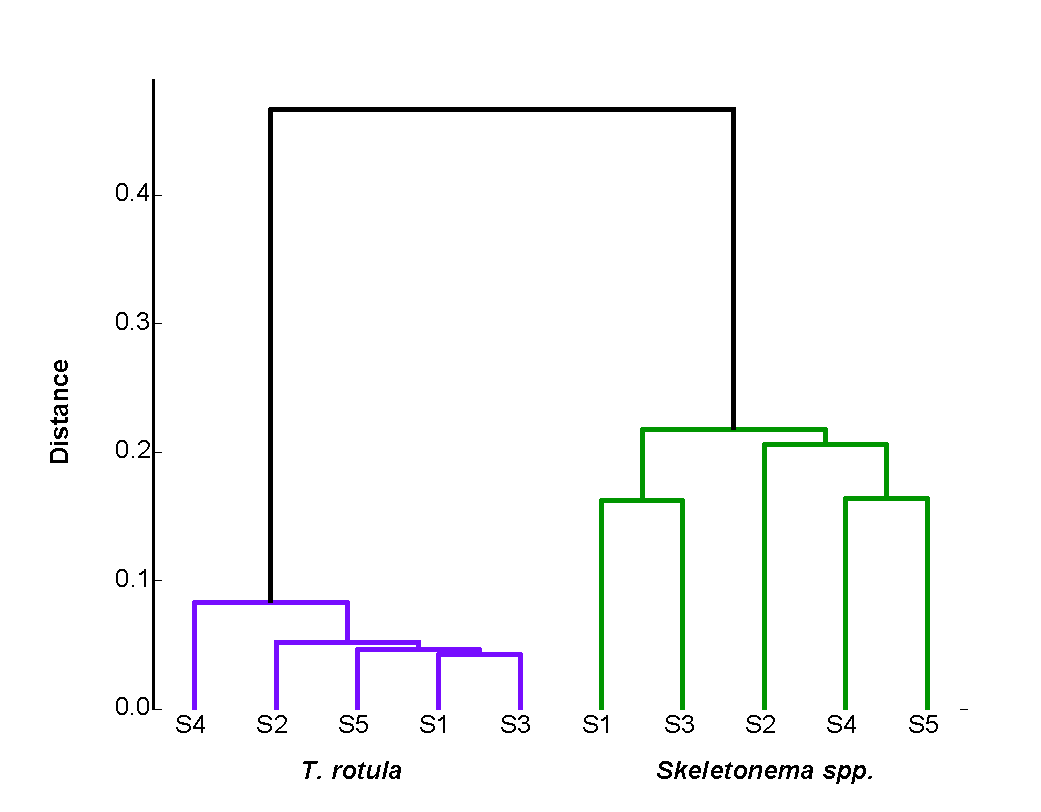
\includegraphics[width=1\textwidth]{Images/C3_SFigure3_Dendrogram.pdf}
    \caption[Hierarchical clustering of QMF signatures across species and samples]{Dendrogram depicting hierarchical clustering of samples based on relative expression of KEGG modules (Figure 2) across the five samples S1-S5 for \textit{Skeletonema} spp. and \textit{T. rotula}.}
  \label{fig:a3f3}
\end{figure}

%Supplemental Figure 4: Stable gene expression across time
\begin{figure}[p!]
  \centering
    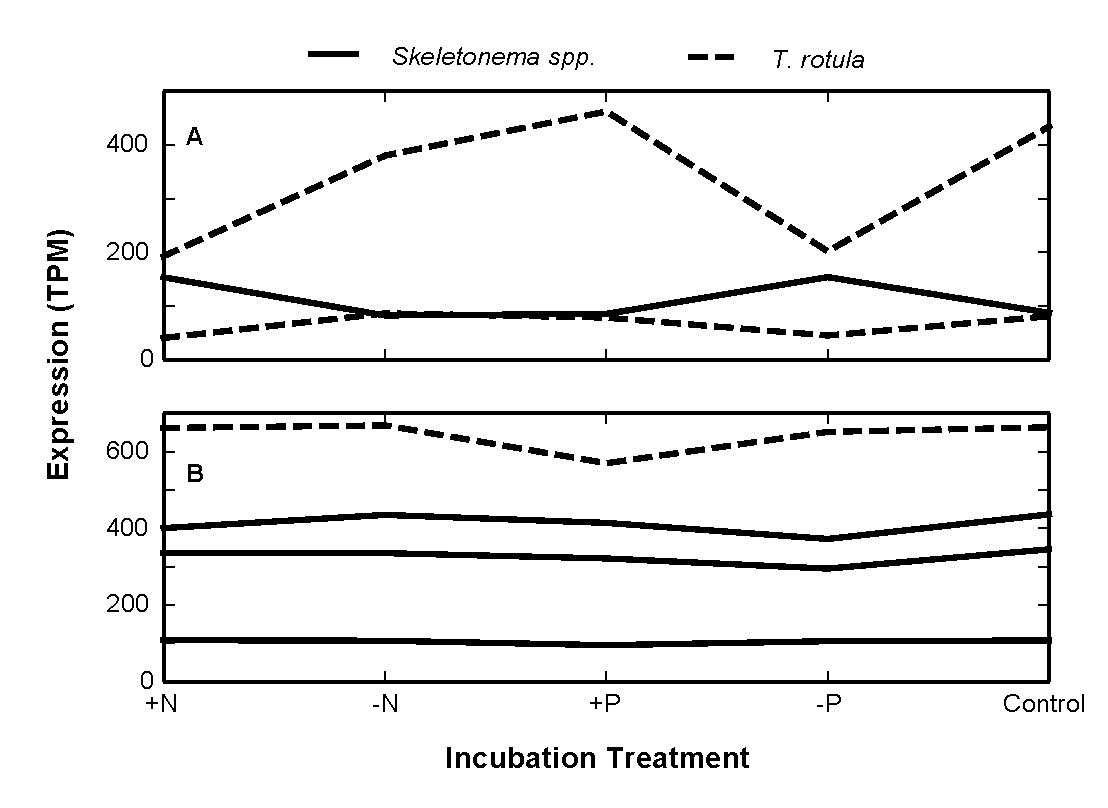
\includegraphics[width=1\textwidth]{Images/C3_SFigure4_StableGenePlot_wActin.pdf}
    \caption[Expression of stable reference genes in the field]{Expression of stable reference genes identified based on literature and statistical parsing in nutrient amendment incubation. (A) The expression in tags per million ($TPM$) of stable reference genes identified in \textit{T. rotula} (dashed line) and \textit{Skeletonema} spp.  (solid lines) based on homology (e-value < 1e-5) to a known reference genes in \textit{T. pseudonana}, ACT1 (Thaps\_25772), in nutrient incubations. (B) Also shown are reference genes identified in the incubation experiments, using statistical analysis of sequence counts \citep{Alexander2012, Wu2010}, and nutrient incubations }
  \label{fig:a3f4}
\end{figure}

%Supplemental Figure 5: RR gene composition
\begin{figure}[p!]
  \centering
    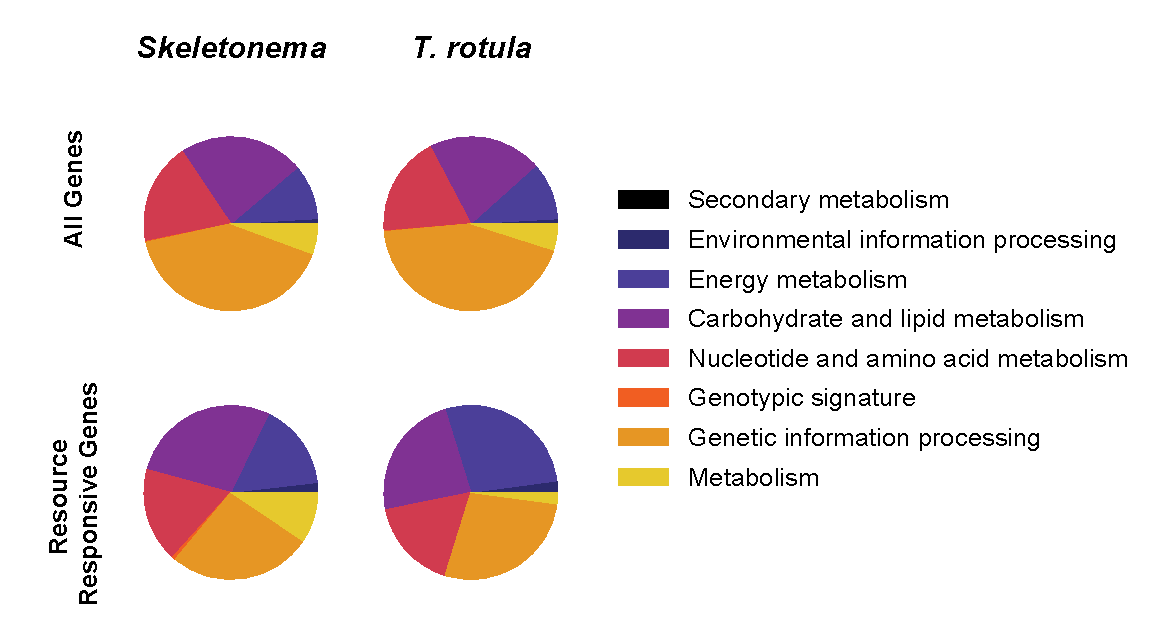
\includegraphics[width=1\textwidth]{Images/C3_SFigure5_RR_All_Genes_Pie.pdf}
    \caption[Functional compoosition of the reference transcriptome and resource-responsive gene sets]{Functional composition of the reference transcriptome and resource-responsive (RR) gene subset for \textit{T. rotula} and \textit{Skeletonema} spp. (A) RR gene sets were identified through cross comparison of like-nutrient incubations (i.e. +N vs. -N and +P vs. -P), using ASC (fold change = 2, post-$p > 0.95$). The relative functional categorization of the reference transcriptomes and RR gene set for \textit{T. rotula} and \textit{Skeletonema} spp. based on KEGG ontology as assigned by KAAS is depicted at the module-level.}
  \label{fig:a3f5}
\end{figure}

%Supplemental Figure 6: Expression of nitrate reductase

\begin{figure}[p!]
  \centering
    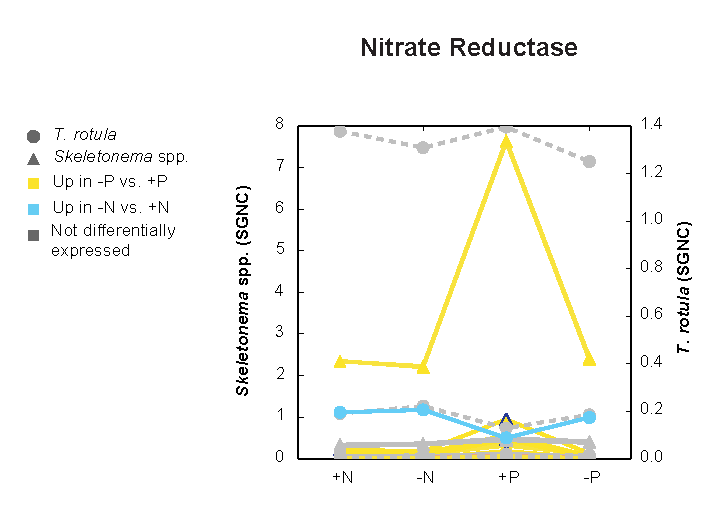
\includegraphics[width=1\textwidth]{Images/C3_SFigure6_SGNC_NitrateReductase.pdf}
    \caption[Relative expression of nitrate reducatses across incubation experiments]{The relative expression in stable gene normalized counts ($SGNC$) of the assimilatory nitrate reductase gene cluster across the incubation experiment treatments. Significance of regulation between the treatments is denoted by the color of the line; organisms are denoted by the shapes of the marker.}
  \label{fig:a3f6}
\end{figure}

%Supplemental Figure 7: Cluster Analysis


\begin{figure}[p!]
  \centering
    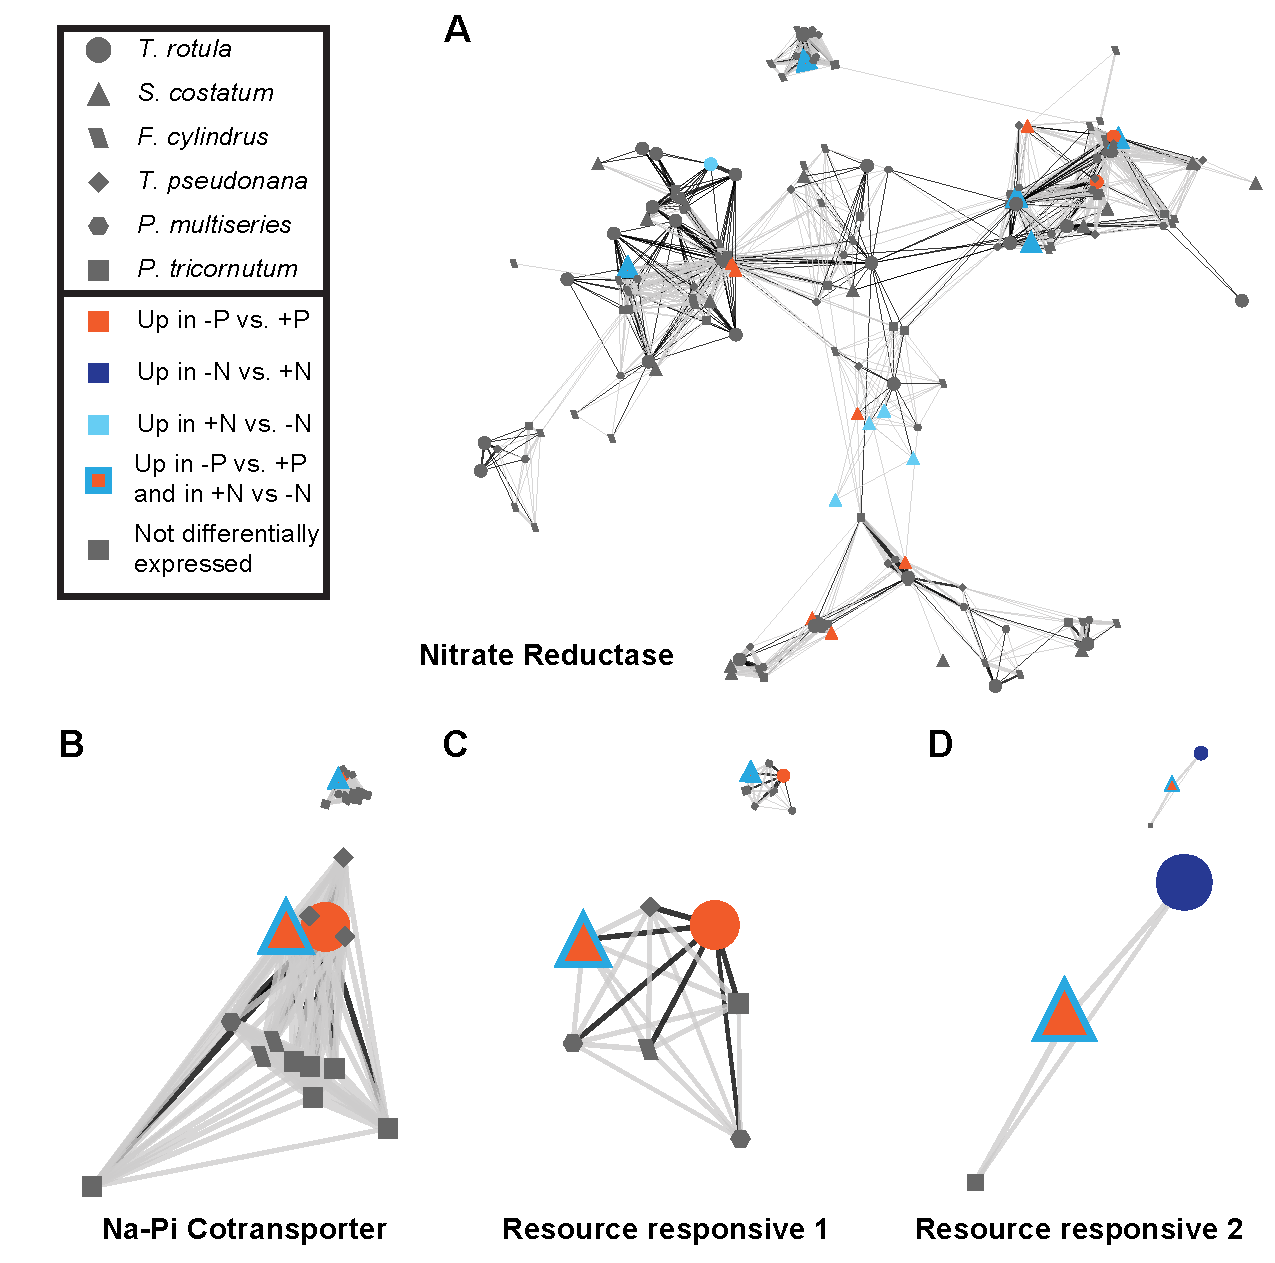
\includegraphics[width=1\textwidth]{Images/C3_SFigure7_ClusterAnalysis_v5.pdf}
    \caption[Gene cluster analysis of nutrient-responsive genes]{Gene cluster known nutrient-responsive genes in \textit{T. pseudonana}: (A) assimilatory nitrate reductase and (B) sodium-phosphate cotransporter and novel resource-responsive (RR) gene families: (C) RR1 and (D) RR2. Transcripts from the transcriptomes of \textit{T. rotula} and \textit{Skeletonema} spp. were clustered based upon relative homology with available diatom genomes: \textit{F. cylindrus}, \textit{P. tricornitum}, \textit{P. multiseries}, and \textit{T. pseudonana}. Symbols indicate different species, while color indicates regulation in the field incubation experiments. Two nodes within a gene cluster are connected by an edge if they share a homologous protein (reciprocal BLAST hit with a minimum of 1e-5 score and minimum 20\% identity). Gene clusters are visualized using an edge-weighted spring-embedded model based on e-value, meaning that genes that are closer together are more similar. The width of the line correlates to the magnitude of the e-value, with lower e-values represented by thicker lines and higher e-values represented by thinner lines.}
  \label{fig:a3f7}
\end{figure}

%Supplemental Figure 8: Conceptual schematic of STD niche space

\begin{figure}[p!]
  \centering
    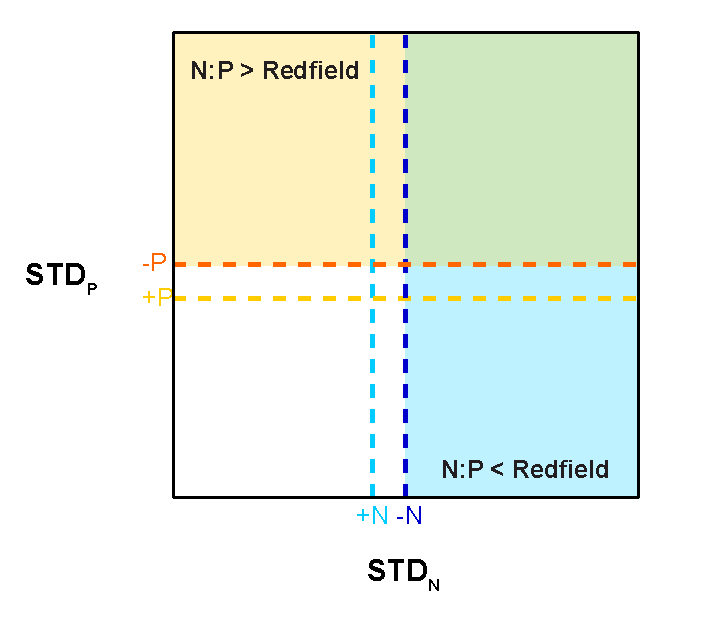
\includegraphics[width=1\textwidth]{Images/C3_SFigure8_Schematic_Quadrants.pdf}
    \caption[Conceptual schemiatic of $STD_N$ plotted against $STD_P$]{A conceptual schematic of $STD_N$ plotted against $STD_P$ hypothesized regions of N:P > Redfield physiology and N:P < Redfield physiology highlighted.}
  \label{fig:a3f8}
\end{figure}


%Supplemental Figure 9: NISP Dn genes
\begin{landscape}
   \centering
   \null         %%<---- this is needed
   \vfill        %%<-----here

	\begin{figure}
  	\centering
    	\includegraphics[width=1.3\textwidth]{Images/C3_SFigure9_NISP_DNGenes.png}
    	\caption[Evolution of niche space indexing over for significantly down-regualted genes]{Evolution of niche space indexing over time in Narragansett Bay for \textit{T. rotula} and \textit{Skeletonema} spp.. The stable gene normalized field signal from genes identified as significantly (2-fold change, post$-p > 0.95$) down-regulated in -P vs +P for Skeletonema spp. (yellow) and \textit{T. rotula} (orange) and in -N vs +N for for \textit{Skeletonema} spp. (cyan) and \textit{T. rotula} (dark blue) was proportionalized relative to the expression for those genes in nutrient incubations, yielding the $STD_N$ and $STD_P$. These data are plotted for Sample 1 through Sample 5.}
  	\label{fig:a3f9}
	\end{figure}
    \vfill        %%<----- and here
\end{landscape}

%Supplemental Figure 10: Percentage of RR genes by quadrant

\begin{figure}[h!]
  \centering
    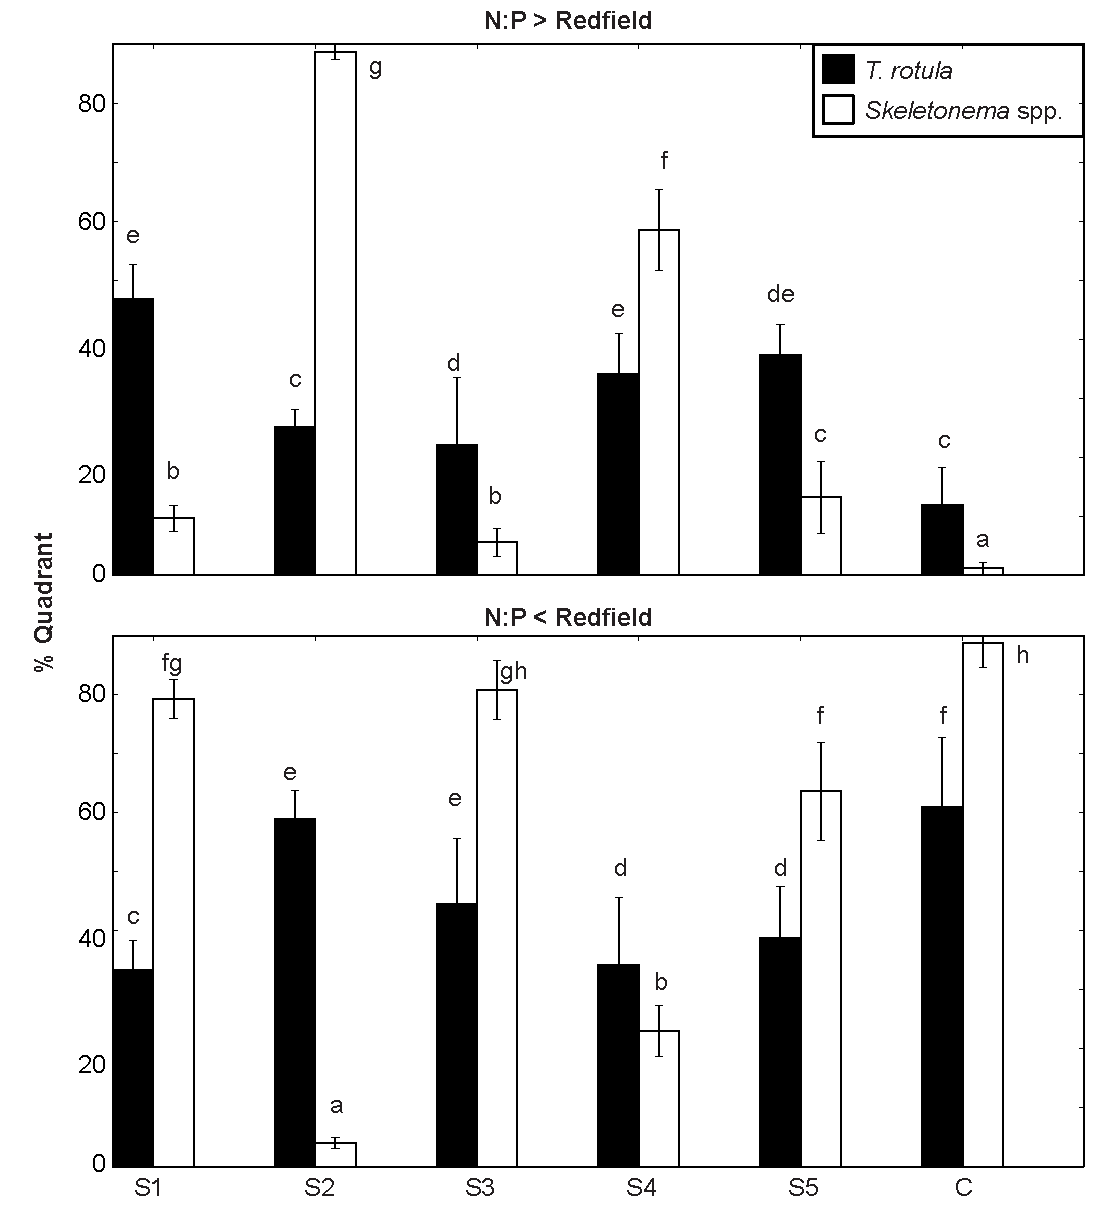
\includegraphics[width=1\textwidth]{Images/C3_SFigure10_BarGraph_Quadrant_2575_stats.pdf}
    \caption[The percentage of identified nutrient responsive genes falling into the N:P > Redfield and N:P < Redfield quadrants with varried cutoffs]{The percentage of identified nutrient responsive genes falling into the N:P > Redfield and N:P < Redfield quadrants for \textit{T. rotula} and \textit{Skeletonema} spp.. The total number of genes falling into the N:P > Redfield quadrant ($STD_P > C$; $STD_N < C$, for $0.25 < C < 0.75$) and the N:P < Redfield quadrant ($STD_P$ < C; $STD_N > C$, for $0.25 < C < 0.75$). The value of C was varied over 10 different values and the average percentages of genes falling into each of the quadrants is depicted above based on the size of the circle at the median $STD_N$ and $STD_P$ for the genes in the quadrant. Similarity of data between species by quadrant was assessed using an analysis of variance (ANOVA) with a generalized linear model. The results from a post hoc Tukey test show the divergence of species across time ($p < 0.05$).}
  \label{fig:a3f10}
\end{figure}

%Supplemental Figure 11: Quadrant localization with varying stable reference genes

\begin{figure}[p!]
  \centering
    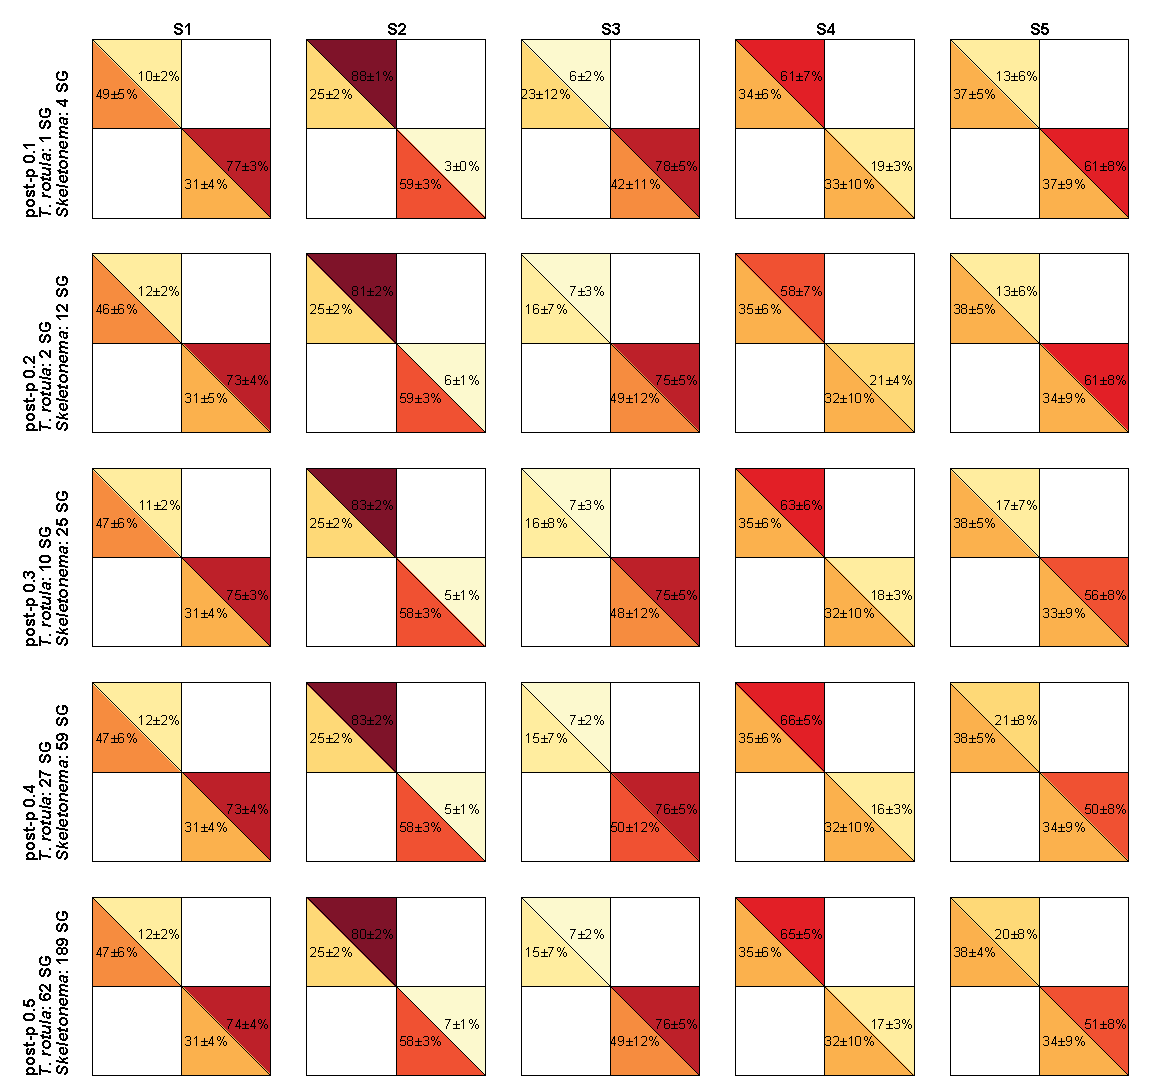
\includegraphics[width=1\textwidth]{Images/C3_SFigure11_Quadrant.pdf}
    \caption[The impact of stable gene selction of quadrant localization]{The impact of stable gene selection on the quadrant localization of the resource responsive gene sets. The posterior probability cutoff used in the selection of stable genes was varied from 0.1 to 0.5 for a fold change of 1.25. The percentage of identified nutrient responsive genes falling into the N:P > Redfield and N:P < Redfield quadrants for \textit{T. rotula} and \textit{Skeletonema} spp. across the five sample points and five posterior probability values is depicted.}
  \label{fig:a3f11}
\end{figure}



\section{Supplemental Tables}

%Supplemental Table 1: library stats

\begin{table}[h!]
\centering
\caption[The total number of paired end reads after quality control and trimming and the percentage of reads mapping]{The total number of paired end reads after quality control and trimming and the percentage of reads mapping to the \textit{T. pseudonana} genome, \textit{T. rotula} transcriptome, and \textit{S. costatum} transcriptome.}
\label{tab:a3t1}

\newcolumntype{C}[1]{>{\centering\let\newline\\\arraybackslash\hspace{.5pt}}m{#1}}

\begin{tabular}{|C{2cm}|C{2.5cm}|C{2.5cm}|C{2.5cm}|C{2.5cm}|}
\hline
\multirow{2}{*}{Sample} & \multirow{2}{*}{\parbox{2.5cm}{Total library size (paired end reads)}} & \multicolumn{3}{c|}{Mapped representation in library} \\ \cline{3-5} 
                        &                                                              & \textit{T. pseudonana}      & \textit{T. rotula}      & \textit{S. costatum}     \\ \hline
S1                      & 89455034                                                     & 2.98\%             & 17.50\%        & 33.50\%         \\ \hline
S2                      & 64888267                                                     & 0.41\%             & 11.70\%        & 54.90\%         \\ \hline
S3                      & 103250243                                                    & 0.39\%             & 7.30\%         & 9.00\%          \\ \hline
S4                      & 45370867                                                     & 0.68\%             & 8.80\%         & 8.30\%          \\ \hline
S5                      & 55061692                                                     & 0.88\%             & 10.40\%        & 11.20\%         \\ \hline
Ambient Control         & 51508197                                                     & 0.27\%             & 13.40\%        & 8.00\%          \\ \hline
+N                      & 58626239                                                     & 0.43\%             & 6.10\%         & 5.30\%          \\ \hline
-N                      & 44561851                                                     & 0.41\%             & 8.70\%         & 8.30\%          \\ \hline
+P                      & 51130364                                                     & 0.29\%             & 8.50\%         & 8.00\%          \\ \hline
-P                      & 58834022                                                     & 0.40\%             & 6.60\%         & 6.50\%          \\ \hline
\end{tabular}
\end{table}

%Supplememntal Table 2: nutrient concentrations used in incubations

\begin{table}[h!]
\centering
\caption[Nutrient concentrations used in nutrient amendment incubations. ]{Nutrient concentrations used in nutrient amendment incubations.}
\label{tab:a3t2}
\begin{tabular}{|c|c|c|c|c|c|}
\hline
                                    & \multicolumn{5}{c|}{\textbf{Treatment}}                                                                                              \\ \cline{2-6} 
\multirow{-2}{*}{\textbf{Nutrient}} & Ambient Control          & + P                      & + N                      & - P                      & - N                      \\ \hline
Nitrate                             & \cellcolor[HTML]{C0C0C0} & \cellcolor[HTML]{C0C0C0} & 10 $\mu M$                    & 10 $\mu M$                    & \cellcolor[HTML]{C0C0C0} \\ \hline
Phosphate                           & \cellcolor[HTML]{C0C0C0} & 3 $\mu M$                     & \cellcolor[HTML]{C0C0C0} & \cellcolor[HTML]{C0C0C0} & 3 $\mu M$                     \\ \hline
Silica                             & \cellcolor[HTML]{C0C0C0} & \cellcolor[HTML]{C0C0C0} & \cellcolor[HTML]{C0C0C0} & 68 $\mu M$                    & 68 $\mu M$                    \\ \hline
Iron                                & \cellcolor[HTML]{C0C0C0} & \cellcolor[HTML]{C0C0C0} & \cellcolor[HTML]{C0C0C0} & 4.6 $\mu M$                   & 4.6 $\mu M$                   \\ \hline
Vitamins                            & \cellcolor[HTML]{C0C0C0} & \cellcolor[HTML]{C0C0C0} & \cellcolor[HTML]{C0C0C0} & f/5                      & f/5                      \\ \hline
\end{tabular}
\end{table}


%Supplememntal Table 3: nutrient concentrations used in incubations

\begin{table}[h!]
\centering
\caption[Mapping statistics for \textit{T. rotula} and \textit{S. costatum} transcriptomes]{Total number of contigs in the \textit{T. rotula} and \textit{S. costatum} transcriptomes and the number of genes in each of the differentially regulated and stable groupings.}
\label{tab:a3t3}
\begin{tabular}{|l|l|l|}
\hline
                                                                       & \textit{\textbf{T. rotula}} & \textit{\textbf{S. costatum}} \\ \hline
Number of contigs in transcriptome                                     & 22362                       & 27665                         \\ \hline
Pass 2 TPM cutoff                                                      & 4318                        & 20921                         \\ \hline
Up in -P vs +P                                                         & 249                         & 4754                          \\ \hline
Down in -P vs +P                                                       & 335                         & 52                            \\ \hline
Up in -N vs +N                                                         & 196                         & 9                             \\ \hline
Down in -N vs +N                                                       & 49                          & 1631                          \\ \hline
All differentially regulated (2 fold change, post-$p > 0.95$) & 775                         & 5136                          \\ \hline
Stable genes (1.25 fold change, post-$p < 0.1$)                  & 1                           & 4                             \\ \hline
\end{tabular}
\end{table}

\clearpage

\section{Supplemental Data}

    \begin{DS3}
    
    \item \label{DS31}: Annotations based on KEGG Ontology for \textit{Skeletonema} spp. and \textit{T. rotula} transcriptomes. \href{http://www.pnas.org/content/suppl/2015/04/09/1421993112.DCSupplemental/pnas.1421993112.sd01.xlsx}{Data Sheet 3-1} can be downloaded from the online version of the manuscript of \citet{Alexander2015} through \href{http://www.pnas.org/content/112/17/E2182.full}{\textit{Proceedings of the National Academy of Sciences}}. 
    \item \label{DS32}: Relative expression in tags per million (TPM) for genes identified as differentially or stably expressed in nutrient incubations. \href{http://www.pnas.org/content/suppl/2015/04/09/1421993112.DCSupplemental/pnas.1421993112.sd02.xlsx}{Data Sheet 3-2} can be downloaded from the online version of the manuscript of \citet{Alexander2015} through \href{http://www.pnas.org/content/112/17/E2182.full}{\textit{Proceedings of the National Academy of Sciences}}. 
  
    \end{DS3}



%%%%%%%%%%%%%%%%%%%%%%%%%%%

%%%%%%%%%%%%%%%%%%%%%%%%%%%_________________CHAPTERFOUR_________________%%%%%%%%%%%%%%%%%%%%%%%%%%%

%%%%%%%%%%%%%%%%%%%%%%%%%%%

\chapter{Chapter 4 Supplemental Information}
\label{sec:app4}
\clearpage
\section{Supplemental Figures}

%Supplemental Figure 1: Chlorophyll values in experiments and in situ samples 
\begin{figure}[h!]
  \centering
    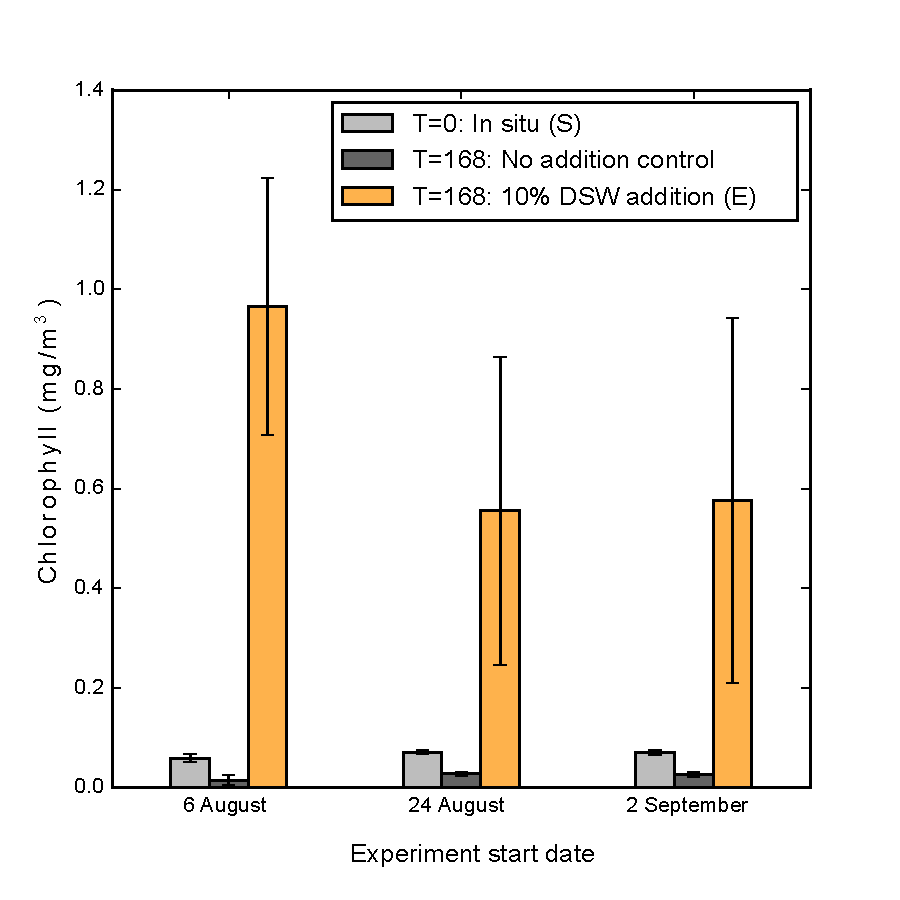
\includegraphics[width=1\textwidth]{Images/C4_FigureS1.pdf}
    \caption[Chlorophyll a of replicated experiments for \emph{in situ} samples, no addition control, and a 10\% deep seawater amendment]{Chlorophyll a of replicated experiments for \emph{in situ} samples (S), a no addition control, and a 10\% deep seawater (DSW) amendment (E). Incubation samples were harvested after 168 hours.}
  \label{fig:a4f1}
\end{figure}


%Supplemental Figure 2: Rank abundance shifts in species composition of diatoms, haptophytes and dinoflagellates

\begin{landscape}
 %  \null         %%<---- this is needed
   \vfill        %%<-----here
\begin{figure}[p!]
  \centering
    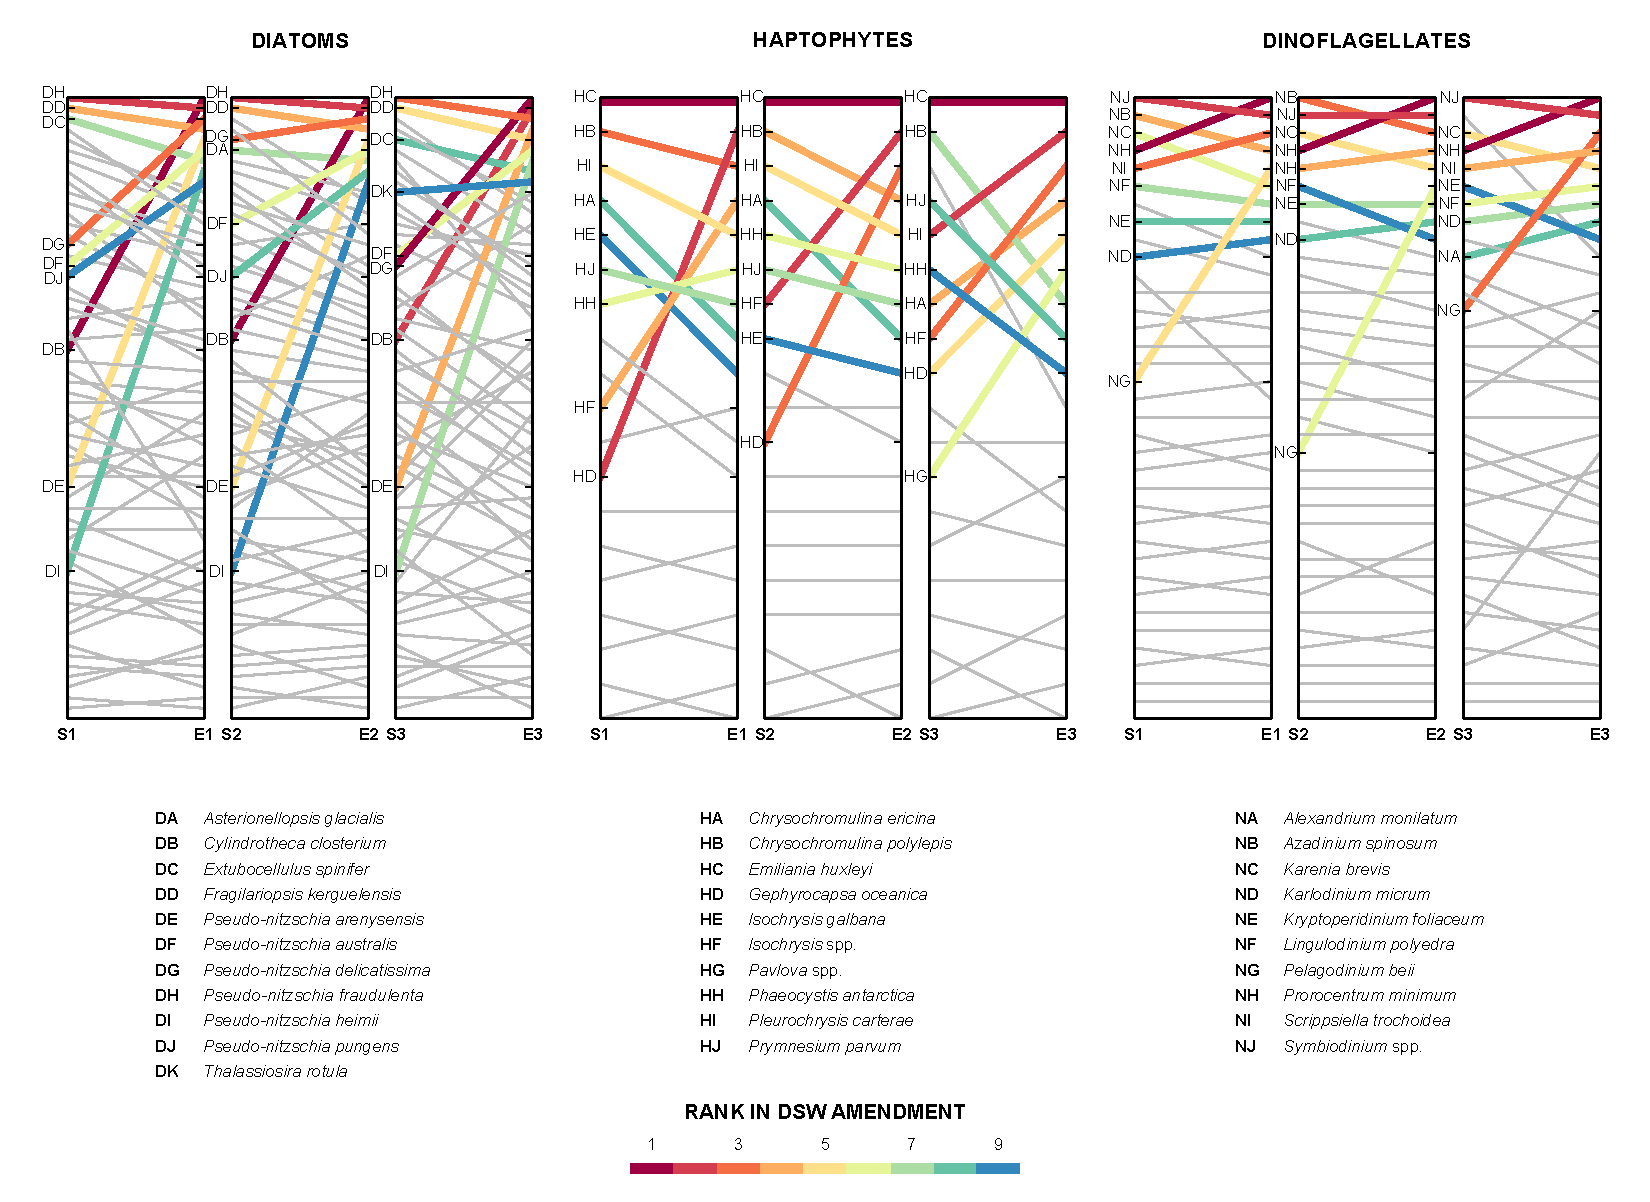
\includegraphics[width=1\textwidth]{Images/C4_FigureS2.pdf}
    \caption[Rank abundance shifts in the species composition of diatoms, haptophytes and dinoflagellates]{Rank abundance shifts in the species composition of diatoms, haptophytes and dinoflagellates for the three experiments. The relative shift in rank abundance for each species is depicted for each incubation experiment (E1-E3) following deep seawater (DSW) addition. The nine most abundant taxa following DSW addition are highlighted for each of the functional groups. Although the species that recruited the reads are denoted here this is highly driven by the composition of the database and does not necessarily indicate the actual species present, but rather the closest species present in the database.}
  \label{fig:a4f2}
\end{figure}
    \vfill        %%<----- and here
\end{landscape}


%Supplemental Figure 3: QMF Comparison across species


\begin{figure}[p!]
  \centering
    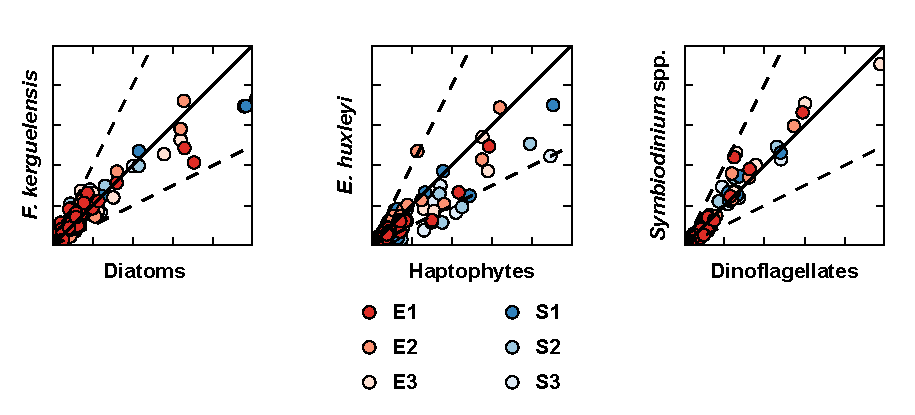
\includegraphics[width=1\textwidth]{Images/C4_FigureS3.pdf}
    \caption[Comparison of the quantitative metabolic fingerprint (QMF) between the whole functional group and representative taxa]{Comparison of the quantitative metabolic fingerprint (QMF) between the whole functional group and representative taxa. The proportion of reads falling into each of the modules depicted in Figure 2 is plotted for S1-S3 and E1-E3, comparing the summed functional group signal and that of a representative taxon. Color of the marker indicates the sample; solid and dashed lines mark the 1:1 and 1:2 lines, respectively.}
  \label{fig:a4f3}
\end{figure}

%Supplemental Figure 4: Distribution histogram

\begin{figure}[p!]
  \centering
    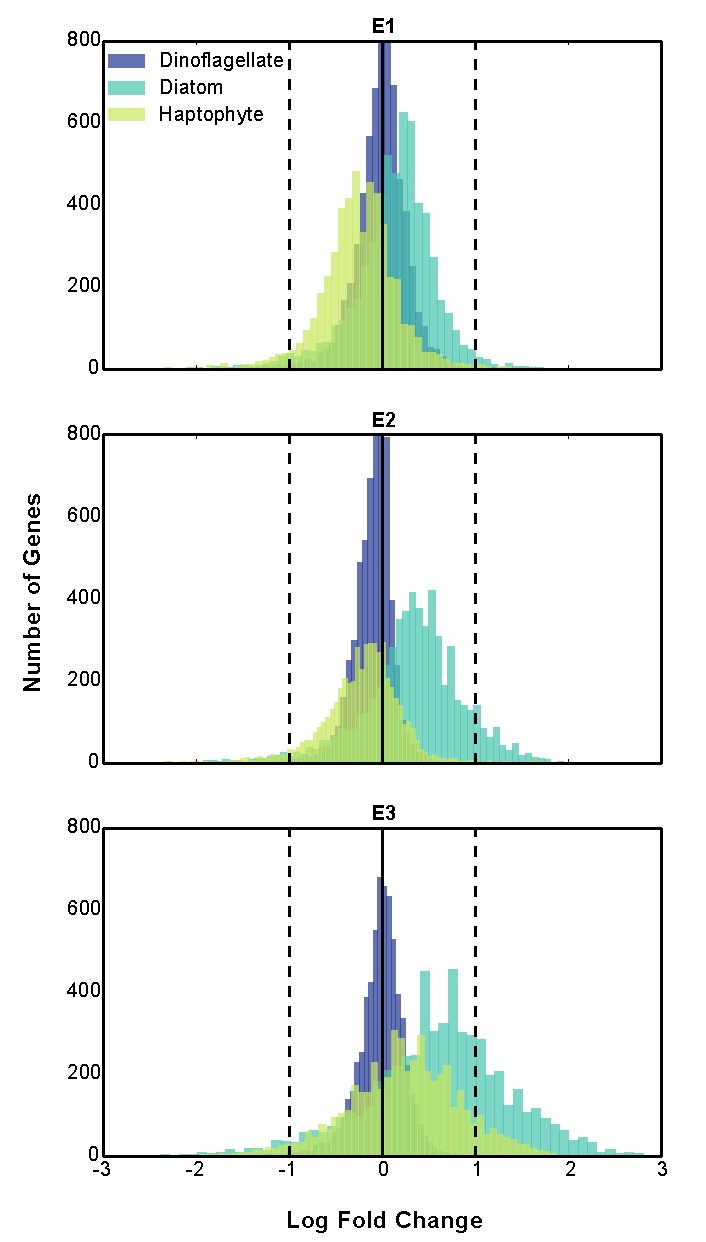
\includegraphics[width=.75\textwidth]{Images/C4_FigureS4.png}
    \caption[Distribution of log fold change following deep seawater (DSW) addition]{Distribution of log fold change following deep seawater (DSW) addition. Histogram of the number of genes falling within each of the log fold change bins for diatoms, haptophytes and dinoflagellates. Solid line indicates no fold change; dashed lines indicate 2 fold-change both up and down.}
  \label{fig:a4f4}
\end{figure}


%Supplemental Figure 5: Weight venn diagrams for up and down regulated genes

\begin{figure}[p!]
  \centering
    \includegraphics[width=1\textwidth]{Images/C4_FigureS5.pdf}
    \caption[Weighted Venn diagrams of genes with significantly different abundances following deep seawater (DSW) addition by functional group]{Weighted Venn diagrams of genes with significantly different abundances following deep seawater (DSW) addition by functional group. The uniqueness of KEGG orthologs with increased or decreased abundances as determined by ASC (2 fold-change, post-p > 0.95) across experiments was assessed for diatoms, haptophytes, and dinoflagellates.}
  \label{fig:a4f5}
\end{figure}


%Supplemental Figure 6: MANTA Plots

\begin{figure}[p!]
  \centering
    \includegraphics[width=.7\textwidth]{Images/C4_FigureS6.pdf}
    \caption[Microbial Assemblage Normalized Transcript Analysis (MANTA) ratio-averaged plots for global shifts in expression of KEGG orthologs]{Microbial Assemblage Normalized Transcript Analysis (MANTA) ratio-averaged plots for global shifts in expression of KEGG orthologs. Fold change ratio (R) and average read count (A) are plotted for read counts in the \emph{in situ} (S) and deep seawater (DSW) amendment (E) samples across the three sample pairs (S1:E1, S2:E2, S3:E3). The trimmed mean of fold-change values is noted as a gray solid line; orthologs unique to one library are separated by gray dashed lines. Pies indicate the taxonomic distribution of orthologous reads across the three functional groups. KEGG orthologs that were significantly differentially expressed (DE) (adjusted $P > 0.05$) are outlined in black and those not significantly DE are outlined in gray. DE KEGG orthologs that fall in the Energy Metabolism KEGG module are outlined in orange.}
  \label{fig:a4f6}
\end{figure}

%Supplemental Figure 7: QMF across incubation experiments

\begin{figure}[p!]
  \centering
    \includegraphics[width=1\textwidth]{Images/C4_FigureS7.pdf}
    \caption[Principal component analysis of the quantitative metabolic fingerprint (QMF) signals across \emph{in situ}, no addition control, and deep seawater amended samples]{Principal component analysis of the quantitative metabolic fingerprint (QMF) signals across \emph{in situ}, no addition control, and deep seawater (DSW) amended samples. Principal component analysis of the QMF signals for each of the functional groups across \emph{in situ} (S1-S3), control no addition (C1-C3) and DSW amendment (E1-E3); 95\% confidence ellipses are indicated for each of the sample types by functional group.}
  \label{fig:a4f7}
\end{figure}

\clearpage

\section{Supplemental Tables}

% Supplemental table with nutrient concentrations post treatment run for E and C
\begin{table}[h!]
\centering
\caption[Macronutrient concentrations in deep seawater ammendment and the incubation experiments after 168 hours]{Macronutrient concentrations in control no addition (C), DSW-amended incubations (E), and 700 m water used in DSW amendment incubations}
\label{tab:a4t1}
\newcolumntype{C}[1]{>{\centering\let\newline\\\arraybackslash\hspace{.5pt}}m{#1}}
\begin{tabular}{ccccc}

    
\hline
\multicolumn{1}{|c|}{\multirow{2}{*}{\textbf{Treatment}}} & \multicolumn{1}{c|}{\multirow{2}{*}{\textbf{\begin{tabular}[c]{@{}c@{}}Time post \\ inoculation (hours)\end{tabular}}}} & \multicolumn{1}{c|}{\multirow{2}{*}{\textbf{\begin{tabular}[c]{@{}c@{}}NO$_2$ + NO$_3$ \\ ($\mu M$)\end{tabular}}}} & \multicolumn{1}{c|}{\multirow{2}{*}{\textbf{\begin{tabular}[c]{@{}c@{}}PO$_4$ \\ ($\mu M$)\end{tabular}}}} & \multicolumn{1}{c|}{\multirow{2}{*}{\textbf{\begin{tabular}[c]{@{}c@{}}Si\\ ($\mu M$)\end{tabular}}}} \\

\multicolumn{1}{|c|}{}                                    & \multicolumn{1}{c|}{}                                                        & \multicolumn{1}{c|}{}                                                                                    & \multicolumn{1}{c|}{}                                                                              & \multicolumn{1}{c|}{}                                                                            \\ \hline
\multicolumn{1}{|c|}{\textbf{C} (control no addition) *}  & \multicolumn{1}{c|}{168}                                                     & \multicolumn{1}{c|}{$0.12 \pm 0.03$}                                                                         & \multicolumn{1}{c|}{$0.12 \pm 0.02$}                                                                   & \multicolumn{1}{c|}{$1.91 \pm 0.2$}                                                                  \\ \hline
\multicolumn{1}{|c|}{\textbf{E} (+ 10\% DSW) *}           & \multicolumn{1}{c|}{168}                                                     & \multicolumn{1}{c|}{$1.9 \pm  .93$}                                                                          & \multicolumn{1}{c|}{$0.23 \pm 0.05$}                                                                   & \multicolumn{1}{c|}{$8.46 \pm 3.11$}                                                                 \\ \hline
\multicolumn{1}{|c|}{\textbf{DSW} (700 m water) *}        & \multicolumn{1}{c|}{N/A}                                                     & \multicolumn{1}{c|}{$37.5 \pm 1.68$}                                                                         & \multicolumn{1}{c|}{$3.14 \pm 0.03$}                                                                   & \multicolumn{1}{c|}{$83.4 \pm 9.33$}                                                                 \\ \hline
\multicolumn{5}{l}{\textit{* Nutrient data averaged for E1 and E2, nutrients were not assayed on E3.}}                                                                                                                                                                                                                                                                                                                                                     
\end{tabular}
\end{table}


\chapter{Chapter 5 Supplemental Information}
\clearpage
\section{Supplemental Figures}


%Supplemental Figure 8: Shifts in CORE

\begin{figure}[h!]

  \centering
  \includegraphics[width=1\textwidth]{Images/C6_FigureS8_core_genes.pdf}
  \caption[The relative expression of `core', shared, and CCMP1516-specific transcripts across time and in incubation experiments]{The relative expression of `core', shared, and CCMP1516-specific transcripts across time and in incubation experiments. The percentage of all mapped reads corresponding to the genes considered to be `core' by Read et al. (2013) (black), found to be shared across the five strains used in this study (grey), or originally considered to be unique to CCMP1516 are plotted for each \textit{in situ} sample (A) and in each of the two replicated incubation experiments, E1 (B) and E2 (C). Nutrients added to incubation experiments are indicated on the exterior of the radar plots, indicating the addition of nitrate, phosphate, trace metals, and vitamins.}
    \label{fig:a5f8}
\end{figure}




%Supplemental Figure 1: Nutrient concentrations at Tf

\begin{figure}[h!]
  \centering
    \includegraphics[width=.6\textwidth]{Images/C6_FigureS1_nutrients_v1.pdf}
    \caption{Inorganic nitrogen and phosphorus concentrations at the point of RNA sampling (7 days post-inoculation) for each of the six treatments in E1 and E2, averaged across triplicate bottles (n=3).}
    \label{fig:a5f1}
\end{figure}


%Supplemental Figure 2: KOG distributions across genes

\begin{figure}[p!]
  \centering
    \includegraphics[width=1.0\textwidth]{Images/C6_FigureS2_KOG_Distribution}
    \caption{The percent of genes falling into each of the KOG classes for each of the five strains.}
    \label{fig:a5f2}
\end{figure}

%Supplemental Figure 3: Distributions across genes

\begin{figure}[p!]
  \centering
    \includegraphics[width=1.0\textwidth]{Images/C6_FigureS3_GeneDistrubtion.pdf}
    \caption[The number of orthologous groups falling into each of the possible strain sets across the five strains surveyed]{The number of orthologous groups falling into each of the possible strain sets across the five strains surveyed. The relative strain membership is depicted in a scatter plot along the x-axis ranging from the first row of 'shared' or `core' genes, common to all strains (black), through variable memberships across some but not all strains, to sets comprised of only one strain (colored). Genes common to all strains in this study are shown in black. Genes identified as `core' in CCMP1516, the genome strain, by Read et al. (2013), but that were not identified in some or all of the other strains were added to the `shared' set and are indicated in yellow hatching. }
    \label{fig:a5f3}
\end{figure}


%Supplemental Figure 4: MANTA

\begin{figure}[p!]
  \centering
    \includegraphics[width=0.8\textwidth]{Images/C6_FigureS4_MANTA.png}
    \caption[Log normalized fold change plotted against log normalized average abundance for each of the five amended treatments compared to the no-addition control]{Log normalized fold change plotted against log normalized average abundance for each of the five amended treatments compared to the no-addition control. edgeR was used to assess the average abundance and log fold change for each of the orthologous groups (left column) and strain-specific transcripts (right column). Genes are colored by generalized metabolic function. The intensity of the color indicates significance, with opaque indicating significance (FDR < 0.05). }
    \label{fig:a5f4}
\end{figure}


%Supplemental Figure 5: Venn 

\begin{figure}[p!]
  \centering
    \includegraphics[width=0.8\textwidth]{Images/C6_FigureS5_Venn_DEGenes.pdf}
    \caption[Weighted Venn diagrams of significantly different, increased, and decreased orthologus groups and species-specific transcripts across each of the amendedments to which N was added. ]{Weighted Venn diagrams of significantly (FDR $< 0.05$) different, increased, and decreased orthologus groups and species-specific transcripts across each of the amendments to which N was added (+N, -P, +DSW).}
    \label{fig:a5f5}
\end{figure}

%Supplemental Figure 6: Carbon, Nucleotide etc. 


\begin{figure}[p!]

  \centering
  \includegraphics[width=1\textwidth]{Images/C6_FigureS6_MckewCarbon.pdf}
    \caption[Fold change of genes associated with carbon, nucleotide, and amino acid metabolism across each of the incubation amendments]{Fold change of genes associated with carbon, nucleotide, and amino acid metabolism across each of the incubation amendments compared to the no addition control. The log fold change of orthologous groups associated with carbon, nucleotide, and amino acid metabolism was assessed with edgeR across the five amended incubations compared to the no addition control are plotted in opaque grey. The size of the orthologous group marker is proportionate to the log of the mean abundance across the two treatments. Orthologous groups are that are significantly differentially abundant (FDR < 0.05) are plotted highlighted in red. Individual transcripts within an orthologous group are plotted in light grey or red to indicate significance of fold change. Genes of interest are labeled with abbreviations as follows, labels in bold indicate significant regulation in two or more conditions. }
    \label{fig:a5f6}
\end{figure}

%Supplemental Figure 7: ATP

\begin{figure}[p!]

  \centering
  \includegraphics[width=1\textwidth]{Images/C6_FigureS7_MckewATP.pdf}
    \caption[Fold change of genes associated with photosynthesis, ATP synthesis, Calvin cycle, TCA cycle, and glycolysis across each of the incubation amendments]{Fold change of genes associated with photosynthesis, ATP synthesis, Calvin cycle, TCA cycle, and glycolysis across each of the incubation amendments compared to the no addition control. The log fold change of orthologous groups associated with photosynthesis, ATP synthesis, Calvin cycle, TCA cycle, and glycolysis was assessed with edgeR across the five amended incubations compared to the no addition control are plotted in opaque grey. The size of the orthologous group marker is proportionate to the log of the mean abundance across the two treatments. Orthologous groups are that are significantly differentially abundant (FDR < 0.05) are plotted highlighted in red. Individual transcripts within an orthologous group are plotted in light grey or red to indicate significance of fold change. Genes of interest are labeled with abbreviations as follows, labels in bold indicate significant regulation in two or more conditions. }
    \label{fig:a5f7}
\end{figure}



%Supplemental Figure 9: Annotation of Core

\begin{figure}[p!]

  \centering
  \includegraphics[width=.75\textwidth]{Images/C6_FigureS9_KOGAnnotation.pdf}
  \caption[Annotation of orthologous groups using KOG orthology for all \textit{E. huxleyi} orthologous groups and for shared orthologous groups]{Annotation of orthologous groups using KOG orthology for all \textit{E. huxleyi} orthologous groups and for shared orthologous groups. The relative percentage of orthologous groups able to be annotated for all orthologous groups (A) and orthologous group shared amongst the five studied strains (B) are shown. The number of orthologous groups falling into each KOG class or multiple classes (m.c.) is shown for both all orthologous groups (C) and shared groups (D). }
    \label{fig:a5f9}
\end{figure}


%Supplemental Figure 10: Strain composition of the shared gene set in the field


\begin{figure}[p!]

  \centering
  \includegraphics[width=1\textwidth]{Images/C6_FigureS10_SharedGeneComp.pdf}
  \caption[RSEM estimated contribution of each strain to the abundance of the shared set of genes in the field and incubation experiments]{RSEM estimated contribution of each strain to the abundance of the shared set of genes in the field and incubation experiments.}
    \label{fig:a5f10}
\end{figure}
\clearpage

\section{Supplemental Tables}

\begin{table}[h!]
\centering
\caption{Final nutrient concentrations used in nutrient amendment incubations.}
\label{tab:c5t1}
\small
\begin{tabular}{lllllll}
                              & \multicolumn{6}{c}{\textbf{Treatment}}                                                   \\ 
\textbf{Amendment}            & \textbf{Control} & \textbf{+N} & \textbf{+P} & \textbf{-N} & \textbf{-P} & \textbf{+DSW} \\ \Xhline{2\arrayrulewidth}
\textbf{Nitrate}              & -                & $4 \mu M$   & -           & -           & $4 \mu M$   & -             \\ 
\textbf{Phosphate}            & -                & -           & $3 \mu M$   & $3 \mu M$   & -           & -             \\ 
\textbf{Silica}               & -                & -           & -           & $8.7 \mu M$ & $8.7 \mu M$ & -             \\ 
\textbf{Iron}                 & -                & -           & -           & $5 nM$      & $5 nM$      & -             \\ 
\textbf{Vitamin B$_{12}$}     & -                & -           & -           & $100 pM$    & $100 pM$    & -             \\ 
\textbf{Deep Seawater (700m)} & -                & -           & -           & -           & -           & 10\% v/v      \\ 
\end{tabular}
\end{table}

\begin{landscape}
\begin{table}[h!]
\centering
\caption{Strain isolation date, synonyms, and transcriptome/genome information for each of the five strains used in this study.}
\label{tab:c5t2}
\small
\newcolumntype{L}[1]{>{\raggedright\let\newline\\\arraybackslash\hspace{0pt}}m{#1}}
\begin{tabular}{lL{1.25cm}L{2cm}L{2.5cm}L{2cm}L{2cm}L{2cm}L{3cm}L{3cm}}
\hline
\textbf{Strain}   & \textbf{Isolation date} & \textbf{Strain synonyms}                  & \textbf{Genome or Transcriptome} & \textbf{Predicted proteins} & \textbf{Transcripts passing quality control} & \textbf{Representative orthoMCL orthologus groups} & \textbf{MMETSP Sample IDs} & \textbf{Reference for genome/ transcriptome download}      \\ \Xhline{2\arrayrulewidth}

\textbf{CCMP1516} & 1991                    & CCMP2090                                  & Genome                           & 33341                                         & 32538                                        & 23792                                              & N/A                        & \href{http://genome.jgi.doe.gov/Emihu1/Emihu1.download.ftp.html}{JGI} \\ \hline
\textbf{CCMP370}  & 1959                    & 451B, F451                                & Transcriptome                    & 38712                                         & 33455                                        & 29068                                              & MMETSP1154-1157            & \href{http://data.imicrobe.us/combined\_assembly/view/34}{iMicrobe}        \\ \hline
\textbf{CCMP374}  & 1990                    & 89E, CCMP1949                             & Transcriptome                    & 18859                                         & 15728                                        & 14628                                              & MMETSP1006-1009            & \href{http://data.imicrobe.us/combined\_assembly/view/32}{iMicrobe}        \\ \hline
\textbf{CCMP379}  & 1957                    & 92A, P-92A, UTEX1061, CCAP/1A, Plymouth 2 & Transcriptome                    & 23300                                         & 20016                                        & 18561                                              & MMETSP0994-0997            & \href{http://data.imicrobe.us/combined\_assembly/view/33}{iMicrobe}        \\ \hline
\textbf{PLYM219}  & 1992                    & NZEH, CAWPO 6                             & Transcriptome                    & 36189                                         & 31410                                        & 27741                                              & MMETSP1150-1153            & \href{http://data.imicrobe.us/combined\_assembly/view/35}{iMicrobe}        \\ \hline

\end{tabular}
\end{table}
\end{landscape}





\begin{landscape}
\begin{center}


    \begin{footnotesize}
    
        \begin{longtable}{|p{0.5cm}|p{1.5cm}|p{4cm}|l|l|l|l|l|l|l|}

\caption{My caption}
\label{my-label}
\hline
\textbf{ID}  & \textbf{Orthologus Group} & \textbf{Transcripts}                                                                                                                                                                                                                                                                                                                                                                                                                                                                                                                                                                                                                     & \textbf{log2(+N/Control)} & \textbf{FDR} & \textbf{log2(-P/Control)} & \textbf{FDR} & \textbf{log2(+DSW/Control)} & \textbf{FDR} & \textbf{Manual Annotation}                                                   \\ \hline


\endhead

\textbf{N0}  & OG1\_5\_21653 & Emi379|CAMPEP\_0187631064; Emihu1|102453                                                                                                                                                                                                                                                                                                                                                                                                                                                                                                                                                                                                 & -9.04E+00 & 6.21E-04 & -3.42E+00 & 5.43E-02 & -8.96E+00 & 6.02E-04 & Amidase; indole acetamide hydrolase                                          \\ \hline
\textbf{N1}  & OG1\_5\_3553  & Emi374|CAMPEP\_0187600766; Emi370|CAMPEP\_0187661076; Emi370|CAMPEP\_0187667014; Emihu1|219042; Emihu1|219043; Emihu1|219044                                                                                                                                                                                                                                                                                                                                                                                                                                                                                                             & -5.91E+00 & 2.46E-03 & -3.15E+00 & 6.48E-02 & -6.54E+00 & 3.27E-03 & Acetamidase/Formamidase                                                      \\ \hline
\textbf{N2}  & OG1\_5\_1624  & Emi374|CAMPEP\_0187579668; Emi379|CAMPEP\_0187646452; Emi370|CAMPEP\_0187734538; Emi219|CAMPEP\_0187763110; Emi219|CAMPEP\_0187800878; Emihu1|469992; Emihu1|245832; Emihu1|453687; Emihu1|215750                                                                                                                                                                                                                                                                                                                                                                                                                                        & -5.59E+00 & 2.81E-02 & -4.24E+00 & 5.32E-02 & -7.88E+00 & 4.16E-02 & Acetamidase/Formamidase                                                      \\ \hline
\textbf{N3}  & OG1\_5\_9478  & Emi374|CAMPEP\_0187586824; Emi370|CAMPEP\_0187667970; Emihu1|452779; Emihu1|451136                                                                                                                                                                                                                                                                                                                                                                                                                                                                                                                                                       & -4.54E+00 & 7.75E-10 & -2.17E+00 & 1.82E-01 & -4.16E+00 & 3.09E-09 & Putative ammonium transporter                                                \\ \hline
\textbf{N4}  & OG1\_5\_4603  & Emi374|CAMPEP\_0187581450; Emi379|CAMPEP\_0187621022; Emi219|CAMPEP\_0187776116; Emihu1|460408; Emihu1|361445; Emihu1|195544                                                                                                                                                                                                                                                                                                                                                                                                                                                                                                             & -3.24E+00 & 8.36E-04 & -3.25E+00 & 5.03E-03 & -3.75E+00 & 2.18E-04 & Nitrate transporter                                                          \\ \hline
\textbf{N5}  & OG1\_5\_6572  & Emi374|CAMPEP\_0187606704; Emi379|CAMPEP\_0187621972; Emi370|CAMPEP\_0187666900; Emi219|CAMPEP\_0187750668; Emihu1|73160                                                                                                                                                                                                                                                                                                                                                                                                                                                                                                                 & -3.11E+00 & 1.12E-01 & -4.38E+00 & 1.05E-01 & -3.93E+00 & 5.67E-02 & Nitrate transporter                                                          \\ \hline
\textbf{N6}  & OG1\_5\_1952  & Emi374|CAMPEP\_0187611660; Emi379|CAMPEP\_0187642306; Emi370|CAMPEP\_0187679516; Emi219|CAMPEP\_0187740072; Emihu1|440751; Emihu1|68140; Emihu1|440179; Emihu1|460978                                                                                                                                                                                                                                                                                                                                                                                                                                                                    & -3.10E+00 & 3.76E-09 & -1.26E+00 & 8.31E-02 & -2.83E+00 & 3.41E-09 & Urea transporter                                                             \\ \hline
\textbf{N7}  & OG1\_5\_13358 & Emi374|CAMPEP\_0187611968; Emi379|CAMPEP\_0187626060; Emi370|CAMPEP\_0187662694; Emihu1|351211                                                                                                                                                                                                                                                                                                                                                                                                                                                                                                                                           & -3.07E+00 & 4.57E-04 & -2.21E+00 & 4.29E-02 & -3.53E+00 & 7.78E-05 & Acetyl-CoA carboxylase                                                       \\ \hline
\textbf{N8}  & OG1\_5\_13949 & Emi374|CAMPEP\_0187585760; Emihu1|444643; Emihu1|440936                                                                                                                                                                                                                                                                                                                                                                                                                                                                                                                                                                                  & -2.35E+00 & 9.61E-01 & 3.94E-01  & 1.00E+00 & -3.10E+00 & 9.39E-01 & Formamidase                                                                  \\ \hline
\textbf{N9}  & OG1\_5\_5714  & Emi374|CAMPEP\_0187587048; Emi379|CAMPEP\_0187621508; Emi370|CAMPEP\_0187678374; Emi219|CAMPEP\_0187750054; Emihu1|423772                                                                                                                                                                                                                                                                                                                                                                                                                                                                                                                & -2.25E+00 & 2.38E-03 & -2.05E+00 & 7.91E-03 & -2.09E+00 & 6.50E-03 & Urease                                                                       \\ \hline
\textbf{N10} & OG1\_5\_18256 & Emi370|CAMPEP\_0187667966; Emi219|CAMPEP\_0187765940; Emihu1|231096                                                                                                                                                                                                                                                                                                                                                                                                                                                                                                                                                                      & -2.03E+00 & 3.67E-01 & -6.17E+00 & 1.49E-01 & -4.73E+00 & 6.45E-02 & Tentative formate/nitrite transporter                                        \\ \hline
\textbf{N11} & OG1\_5\_5040  & Emi379|CAMPEP\_0187644898; Emi370|CAMPEP\_0187696120; Emi219|CAMPEP\_0187752584; Emihu1|52323; Emihu1|72956                                                                                                                                                                                                                                                                                                                                                                                                                                                                                                                              & -1.62E+00 & 1.00E+00 & -1.88E+00 & 1.00E+00 & -3.10E+00 & 1.00E+00 & Glutamine synthetase                                                         \\ \hline
\textbf{N12} & OG1\_5\_2655  & Emi374|CAMPEP\_0187590198; Emi379|CAMPEP\_0187655336; Emi379|CAMPEP\_0187655236; Emi370|CAMPEP\_0187728390; Emi370|CAMPEP\_0187734300; Emi219|CAMPEP\_0187808162; Emihu1|428968                                                                                                                                                                                                                                                                                                                                                                                                                                                          & -1.29E+00 & 3.40E-01 & -1.70E+00 & 6.15E-02 & -1.74E+00 & 6.67E-02 & Ferredoxin-nitrite reductase precursor                                       \\ \hline
\textbf{N13} & OG1\_5\_1326  & Emi374|CAMPEP\_0187589938; Emi374|CAMPEP\_0187606110; Emi374|CAMPEP\_0187579580; Emi379|CAMPEP\_0187646260; Emi379|CAMPEP\_0187648788; Emi370|CAMPEP\_0187689186; Emi370|CAMPEP\_0187698464; Emi219|CAMPEP\_0187786666; Emi219|CAMPEP\_0187739272; Emihu1|225692; Emihu1|467437                                                                                                                                                                                                                                                                                                                                                          & -1.27E+00 & 4.67E-02 & -1.30E+00 & 2.83E-02 & -1.22E+00 & 5.46E-02 & ferredoxin-dependent glutamate synthase                                      \\ \hline
\textbf{N14} & OG1\_5\_36653 & Emihu1|470023                                                                                                                                                                                                                                                                                                                                                                                                                                                                                                                                                                                                                            & -1.10E+00 & 7.84E-01 & -6.79E-01 & 9.63E-01 & -4.60E-01 & 1.00E+00 & glutamine synthetase                                                         \\ \hline
\textbf{N15} & OG1\_5\_2287  & Emi374|CAMPEP\_0187586322; Emi379|CAMPEP\_0187624740; Emi379|CAMPEP\_0187656886; Emi370|CAMPEP\_0187689050; Emi219|CAMPEP\_0187762872; Emi219|CAMPEP\_0187808378; Emihu1|69253                                                                                                                                                                                                                                                                                                                                                                                                                                                           & -7.18E-01 & 7.85E-01 & 3.98E-01  & 1.00E+00 & -2.23E-02 & 1.00E+00 & Glutamine synthetase; GLN1                                                   \\ \hline
\textbf{N16} & OG1\_5\_5519  & Emi379|CAMPEP\_0187621864; Emi370|CAMPEP\_0187722904; Emi370|CAMPEP\_0187701698; Emi219|CAMPEP\_0187750040; Emihu1|437187                                                                                                                                                                                                                                                                                                                                                                                                                                                                                                                & -2.45E-01 & 1.00E+00 & -8.98E-01 & 6.33E-01 & -2.41E-01 & 1.00E+00 & Glutamine synthetase; GLN4                                                   \\ \hline
\textbf{N17} & OG1\_5\_11682 & Emi374|CAMPEP\_0187610426; Emi379|CAMPEP\_0187629508; Emi219|CAMPEP\_0187742636; Emihu1|201096                                                                                                                                                                                                                                                                                                                                                                                                                                                                                                                                           & -1.15E-01 & 1.00E+00 & 3.86E-01  & 1.00E+00 & 5.06E-01  & 1.00E+00 & putative ammonium transporter                                                \\ \hline
\textbf{N18} & OG1\_5\_6398  & Emi374|CAMPEP\_0187592148; Emi379|CAMPEP\_0187621632; Emi370|CAMPEP\_0187681132; Emi219|CAMPEP\_0187757694; Emihu1|217668                                                                                                                                                                                                                                                                                                                                                                                                                                                                                                                & 1.60E-02  & 1.00E+00 & 4.75E-01  & 1.00E+00 & 1.32E-01  & 1.00E+00 & Alipathic amidase                                                            \\ \hline
\textbf{N19} & OG1\_5\_8043  & Emi374|CAMPEP\_0187582726; Emi379|CAMPEP\_0187618148; Emi370|CAMPEP\_0187694666; Emi219|CAMPEP\_0187745866; Emihu1|433753                                                                                                                                                                                                                                                                                                                                                                                                                                                                                                                & 2.72E-01  & 1.00E+00 & -1.91E-01 & 1.00E+00 & 9.17E-02  & 1.00E+00 & Glycine cleavage system protein H                                            \\ \hline
\textbf{N20} & OG1\_5\_4089  & Emi374|CAMPEP\_0187592906; Emi379|CAMPEP\_0187626556; Emi370|CAMPEP\_0187679210; Emi370|CAMPEP\_0187676248; Emi219|CAMPEP\_0187748646; Emihu1|453721                                                                                                                                                                                                                                                                                                                                                                                                                                                                                     & 4.15E-01  & 1.00E+00 & 3.22E-02  & 1.00E+00 & 1.78E-01  & 1.00E+00 & Glutamine-dependant NAD+ Synthase                                            \\ \hline
\textbf{N21} & OG1\_5\_13403 & Emi374|CAMPEP\_0187579542; Emi379|CAMPEP\_0187657778; Emi370|CAMPEP\_0187698244; Emihu1|433762                                                                                                                                                                                                                                                                                                                                                                                                                                                                                                                                           & 6.32E-01  & 6.35E-01 & 1.02E+00  & 1.61E-01 & 9.14E-01  & 2.54E-01 & Glutamate/leucine/phenylalanine/valine dehydrogenases                        \\ \hline
\textbf{N22} & OG1\_5\_1659  & Emi379|CAMPEP\_0187624650; Emi379|CAMPEP\_0187642912; Emi370|CAMPEP\_0187705728; Emi219|CAMPEP\_0187806566; Emihu1|74037; Emihu1|444314; Emihu1|441727; Emihu1|200882; Emihu1|61319                                                                                                                                                                                                                                                                                                                                                                                                                                                      & 8.23E-01  & 5.97E-01 & 1.79E+00  & 5.62E-04 & 1.18E+00  & 8.46E-02 & Putative ammonium transporter; AMT3                                          \\ \hline
\textbf{N23} & OG1\_5\_1884  & Emi219|CAMPEP\_0187752054; Emihu1|471321; Emihu1|49101; Emihu1|71119; Emihu1|456888; Emihu1|234399; Emihu1|193894; Emihu1|415646                                                                                                                                                                                                                                                                                                                                                                                                                                                                                                         & 8.49E-01  & 1.00E+00 & -3.02E-01 & 1.00E+00 & 2.43E-01  & 1.00E+00 & Putative ammonium transporter; AMT5                                          \\ \hline
\textbf{N24} & OG1\_5\_40788 & Emihu1|64817                                                                                                                                                                                                                                                                                                                                                                                                                                                                                                                                                                                                                             & 8.87E-01  & 9.35E-01 & 1.14E+00  & 6.33E-01 & 7.29E-01  & 1.00E+00 & Cystathionine gamma-lyase                                                    \\ \hline
\textbf{N25} & OG1\_5\_8600  & Emi374|CAMPEP\_0187588052; Emi379|CAMPEP\_0187638144; Emi370|CAMPEP\_0187665342; Emi219|CAMPEP\_0187761444; Emihu1|439254                                                                                                                                                                                                                                                                                                                                                                                                                                                                                                                & 1.31E+00  & 4.18E-01 & 1.40E+00  & 3.65E-01 & 1.42E+00  & 3.09E-01 & Putative formate/nitrite transporter; NAR3                                   \\ \hline
\textbf{N26} & OG1\_5\_2556  & Emi379|CAMPEP\_0187648474; Emi370|CAMPEP\_0187697962; Emi370|CAMPEP\_0187689392; Emi370|CAMPEP\_0187711782; Emi219|CAMPEP\_0187743774; Emihu1|469498; Emihu1|449382                                                                                                                                                                                                                                                                                                                                                                                                                                                                      & 1.43E+00  & 7.10E-01 & 2.36E+00  & 1.72E-01 & 2.31E+00  & 1.58E-01 & NADH-glutamate syntase                                                       \\ \hline
\textbf{N27} & OG1\_5\_2882  & Emi374|CAMPEP\_0187592900; Emi379|CAMPEP\_0187615210; Emi370|CAMPEP\_0187692548; Emi370|CAMPEP\_0187719132; Emi219|CAMPEP\_0187736486; Emihu1|365923; Emihu1|72853                                                                                                                                                                                                                                                                                                                                                                                                                                                                       & 1.48E+00  & 2.65E-01 & 1.78E+00  & 6.03E-02 & 1.29E+00  & 3.85E-01 & Asparagine synthase                                                          \\ \hline
\textbf{N28} & OG1\_5\_5439  & Emi374|CAMPEP\_0187583248; Emi379|CAMPEP\_0187621446; Emi370|CAMPEP\_0187660622; Emihu1|464017; Emihu1|432660                                                                                                                                                                                                                                                                                                                                                                                                                                                                                                                            & 1.65E+00  & 8.92E-03 & 1.86E+00  & 5.28E-04 & 1.62E+00  & 4.44E-03 & Tentative ammonium transporter; AMT4                                         \\ \hline
\textbf{N29} & OG1\_5\_7860  & Emi374|CAMPEP\_0187591398; Emi379|CAMPEP\_0187615180; Emi370|CAMPEP\_0187686840; Emi219|CAMPEP\_0187743664; Emihu1|436026                                                                                                                                                                                                                                                                                                                                                                                                                                                                                                                & 1.72E+00  & 4.60E-02 & 7.93E-01  & 6.78E-01 & 1.66E+00  & 4.73E-02 & glutamine synthetase type III                                                \\ \hline
\textbf{N30} & OG1\_5\_6301  & Emi374|CAMPEP\_0187604472; Emi379|CAMPEP\_0187628134; Emi370|CAMPEP\_0187702136; Emi219|CAMPEP\_0187801324; Emihu1|461482                                                                                                                                                                                                                                                                                                                                                                                                                                                                                                                & 1.89E+00  & 7.79E-01 & 1.11E+00  & 1.00E+00 & 1.86E+00  & 8.69E-01 & Oxioreductase                                                                \\ \hline
\textbf{N31} & OG1\_5\_2557  & Emi374|CAMPEP\_0187578242; Emi379|CAMPEP\_0187649242; Emi379|CAMPEP\_0187638334; Emi370|CAMPEP\_0187683750; Emi219|CAMPEP\_0187763438; Emihu1|70117; Emihu1|433750                                                                                                                                                                                                                                                                                                                                                                                                                                                                       & 2.25E+00  & 4.34E-04 & 2.16E+00  & 2.83E-04 & 2.08E+00  & 1.08E-03 & Putative ammonium transporter;AMT8                                           \\ \hline
\textbf{N32} & OG1\_5\_7463  & Emi374|CAMPEP\_0187591416; Emi379|CAMPEP\_0187615552; Emi370|CAMPEP\_0187679244; Emi219|CAMPEP\_0187748030; Emihu1|212450                                                                                                                                                                                                                                                                                                                                                                                                                                                                                                                & 2.37E+00  & 1.92E-01 & 2.49E+00  & 1.37E-01 & 2.31E+00  & 2.12E-01 & Ferredoxin-dependent glutamate synthase                                      \\ \hline
\textbf{N33} & OG1\_5\_12593 & Emi374|CAMPEP\_0187588360; Emi370|CAMPEP\_0187668054; Emi219|CAMPEP\_0187747110; Emihu1|232873                                                                                                                                                                                                                                                                                                                                                                                                                                                                                                                                           & 2.44E+00  & 3.33E-01 & 1.76E+00  & 1.00E+00 & 2.15E+00  & 5.17E-01 & Thioesterase                                                                 \\ \hline
\textbf{N34} & OG1\_5\_37688 & Emihu1|225018                                                                                                                                                                                                                                                                                                                                                                                                                                                                                                                                                                                                                            & 3.18E+00  & 1.00E+00 & 3.04E+00  & 1.00E+00 & 2.83E+00  & 1.00E+00 & Na+/solute symporter                                                         \\ \hline
\textbf{N35} & OG1\_5\_11710 & Emi374|CAMPEP\_0187599096; Emi370|CAMPEP\_0187734648; Emi219|CAMPEP\_0187770460; Emihu1|422537                                                                                                                                                                                                                                                                                                                                                                                                                                                                                                                                           & 3.29E+00  & 4.38E-02 & 2.02E+00  & 7.40E-01 & 2.89E+00  & 1.74E-01 & Glycine decarboxylase; GDCT1                                                 \\ \hline
\textbf{N36} & OG1\_5\_21588 & Emihu1|210750                                                                                                                                                                                                                                                                                                                                                                                                                                                                                                                                                                                                                            & 4.50E+00  & 1.00E+00 & 2.99E+00  & 1.00E+00 & 3.61E+00  & 1.00E+00 & Nitrilase/cyanide hydratase and apolipoprotein N-acyltransferase             \\ \hline
\textbf{N37} & OG1\_5\_8516  & Emi374|CAMPEP\_0187584190; Emi379|CAMPEP\_0187656468; Emi370|CAMPEP\_0187719494; Emi219|CAMPEP\_0187806644; Emihu1|212114                                                                                                                                                                                                                                                                                                                                                                                                                                                                                                                & 4.77E+00  & 1.00E+00 & 4.82E+00  & 6.32E-01 & 5.13E+00  & 9.67E-01 & Amino acid/polyamine transporter II                                          \\ \hline
\textbf{N38} & OG1\_5\_5632  & Emi374|CAMPEP\_0187612230; Emi370|CAMPEP\_0187683408; Emi370|CAMPEP\_0187725580; Emi219|CAMPEP\_0187766518; Emihu1|69206                                                                                                                                                                                                                                                                                                                                                                                                                                                                                                                 & 4.90E+00  & 1.00E+00 & 3.52E+00  & 1.00E+00 & 3.59E+00  & 1.00E+00 & NADP-specific glutamate dehydrogenase                                        \\ \hline
\textbf{N39} & OG1\_5\_27631 & Emi379|CAMPEP\_0187655464; Emihu1|69043                                                                                                                                                                                                                                                                                                                                                                                                                                                                                                                                                                                                  & 5.90E+00  & 5.92E-01 & 4.98E+00  & 5.73E-01 & 6.89E+00  & 1.85E-01 & histidine ammonia-lyase                                                      \\ \hline
\textbf{N40} & OG1\_5\_7856  & Emi374|CAMPEP\_0187607498; Emi379|CAMPEP\_0187621784; Emi370|CAMPEP\_0187718658; Emi219|CAMPEP\_0187743450; Emihu1|69646                                                                                                                                                                                                                                                                                                                                                                                                                                                                                                                 & 6.75E+00  & 1.34E-01 & 5.21E+00  & 6.33E-01 & 6.83E+00  & 1.16E-01 & Cyanase                                                                      \\ \hline
\textbf{N41} & OG1\_5\_3019  & Emi374|CAMPEP\_0187587786; Emi379|CAMPEP\_0187642606; Emi370|CAMPEP\_0187660896; Emi219|CAMPEP\_0187743856; Emi219|CAMPEP\_0187749342; Emihu1|64600                                                                                                                                                                                                                                                                                                                                                                                                                                                                                      & 7.50E+00  & 1.95E-02 & 5.41E+00  & 5.21E-01 & 6.87E+00  & 1.02E-01 & Putative formate/nitrite transporter;NAR4                                    \\ \hline
\textbf{N42} & OG1\_5\_7714  & Emi374|CAMPEP\_0187610088; Emi379|CAMPEP\_0187624510; Emi370|CAMPEP\_0187666880; Emi219|CAMPEP\_0187784072; Emihu1|106701                                                                                                                                                                                                                                                                                                                                                                                                                                                                                                                & 7.55E+00  & 1.86E-02 & 5.82E+00  & 1.91E-01 & 7.50E+00  & 1.93E-02 & Cystathionine beta-lyase                                                     \\ \hline
\textbf{P0}  & OG1\_5\_9499  & Emi374|CAMPEP\_0187607650; Emi370|CAMPEP\_0187723126; Emihu1|370963; Emihu1|364869                                                                                                                                                                                                                                                                                                                                                                                                                                                                                                                                                       & -1.65E+00 & 4.46E-01 & -2.07E+00 & 2.90E-01 & -2.49E+00 & 1.02E-01 & Hypothetical protein P3TCK                                                   \\ \hline
\textbf{P1}  & OG1\_5\_2434  & Emi374|CAMPEP\_0187586994; Emi370|CAMPEP\_0187667618; Emi219|CAMPEP\_0187805514; Emihu1|456911; Emihu1|67455; Emihu1|67879; Emihu1|450989                                                                                                                                                                                                                                                                                                                                                                                                                                                                                                & 3.36E-01  & 1.00E+00 & 7.69E-02  & 1.00E+00 & -2.54E-01 & 1.00E+00 & Putative inorganic phosphate transporter; PTA11                              \\ \hline
\textbf{P2}  & OG1\_5\_7348  & Emi374|CAMPEP\_0187608816; Emi379|CAMPEP\_0187657498; Emi370|CAMPEP\_0187669144; Emi219|CAMPEP\_0187747478; Emihu1|447541                                                                                                                                                                                                                                                                                                                                                                                                                                                                                                                & 8.23E-01  & 1.00E+00 & 5.28E-01  & 1.00E+00 & 1.11E+00  & 6.91E-01 & Tetrapeptide repeat (TPR) containing protein                                 \\ \hline
\textbf{P3}  & OG1\_5\_3674  & Emi374|CAMPEP\_0187594974; Emi379|CAMPEP\_0187621016; Emi370|CAMPEP\_0187720180; Emi219|CAMPEP\_0187736374; Emihu1|116959; Emihu1|103835                                                                                                                                                                                                                                                                                                                                                                                                                                                                                                 & 7.45E-01  & 1.00E+00 & 6.45E-01  & 1.00E+00 & 8.51E-01  & 1.00E+00 & Phosphotyrosyl phosphatase activator                                         \\ \hline
\textbf{P4}  & OG1\_5\_11629 & Emi374|CAMPEP\_0187576542; Emi370|CAMPEP\_0187671318; Emi219|CAMPEP\_0187747328; Emihu1|61414                                                                                                                                                                                                                                                                                                                                                                                                                                                                                                                                            & 2.01E+00  & 5.69E-01 & 1.03E+00  & 1.00E+00 & 7.30E-01  & 1.00E+00 & Putative inorganic phosphate transporter; PTA7                               \\ \hline
\textbf{P5}  & OG1\_5\_6860  & Emi374|CAMPEP\_0187596730; Emi379|CAMPEP\_0187622668; Emi370|CAMPEP\_0187661946; Emi219|CAMPEP\_0187754422; Emihu1|448031                                                                                                                                                                                                                                                                                                                                                                                                                                                                                                                & 1.72E+00  & 5.86E-01 & 1.61E+00  & 7.89E-01 & 1.71E+00  & 5.42E-01 & 5'-nucleotidase                                                              \\ \hline
\textbf{P6}  & OG1\_5\_5394  & Emi374|CAMPEP\_0187586736; Emi379|CAMPEP\_0187622756; Emi219|CAMPEP\_0187801480; Emihu1|470911; Emihu1|200606                                                                                                                                                                                                                                                                                                                                                                                                                                                                                                                            & 1.98E+00  & 4.12E-01 & 1.85E+00  & 4.28E-01 & 6.87E-03  & 1.00E+00 & Putative phosphate transporter                                               \\ \hline
\textbf{P7}  & OG1\_5\_3301  & Emihu1|119690; Emihu1|228520; Emihu1|111972; Emihu1|111381; Emihu1|214750; Emihu1|202775                                                                                                                                                                                                                                                                                                                                                                                                                                                                                                                                                 & 2.06E+00  & 5.52E-01 & 1.85E+00  & 8.68E-01 & 2.29E+00  & 5.83E-01 & 5'nucleotidase                                                               \\ \hline
\textbf{P8}  & OG1\_5\_14704 & Emi370|CAMPEP\_0187695170; Emi219|CAMPEP\_0187749098; Emihu1|433665                                                                                                                                                                                                                                                                                                                                                                                                                                                                                                                                                                      & 2.31E+00  & 3.79E-03 & 1.86E+00  & 2.53E-02 & 2.25E+00  & 6.65E-03 & Putative alternative oxidase                                                 \\ \hline
\textbf{P9}  & OG1\_5\_26201 & Emi370|CAMPEP\_0187676750; Emihu1|52051                                                                                                                                                                                                                                                                                                                                                                                                                                                                                                                                                                                                  & 4.30E+00  & 1.00E+00 & 2.54E+00  & 1.00E+00 & 4.71E+00  & 1.00E+00 & 5'-nucleotidase                                                              \\ \hline
\textbf{P10} & OG1\_5\_6927  & Emi379|CAMPEP\_0187625566; Emi370|CAMPEP\_0187671440; Emi219|CAMPEP\_0187739966; Emi219|CAMPEP\_0187757248; Emihu1|419488                                                                                                                                                                                                                                                                                                                                                                                                                                                                                                                & 4.25E+00  & 1.00E+00 & 2.54E+00  & 1.00E+00 & 4.49E+00  & 9.67E-01 & Putative inorganic phosphate transporter; PTA5                               \\ \hline
\textbf{P11} & OG1\_5\_3470  & Emi374|CAMPEP\_0187580214; Emi379|CAMPEP\_0187645690; Emi370|CAMPEP\_0187729752; Emi219|CAMPEP\_0187757238; Emihu1|251982; Emihu1|237438                                                                                                                                                                                                                                                                                                                                                                                                                                                                                                 & 5.18E+00  & 9.57E-01 & 2.99E+00  & 1.00E+00 & 5.72E+00  & 6.54E-01 & Putative 5'-nucleotidase; NTD1                                               \\ \hline
\textbf{P12} & OG1\_5\_25996 & Emi370|CAMPEP\_0187667570; Emihu1|434557                                                                                                                                                                                                                                                                                                                                                                                                                                                                                                                                                                                                 & 3.74E+00  & 1.00E+00 & 3.04E+00  & 1.00E+00 & na        & na       & Hypothetical protein; pyruvate phosphate dikinase                            \\ \hline
\textbf{P13} & OG1\_5\_26498 & Emi370|CAMPEP\_0187718564; Emihu1|369509                                                                                                                                                                                                                                                                                                                                                                                                                                                                                                                                                                                                 & 2.85E+00  & 1.00E+00 & 3.33E+00  & 1.00E+00 & na        & na       & Putative alkaline phosphatase                                                \\ \hline
\textbf{P14} & OG1\_5\_2841  & Emi374|CAMPEP\_0187605194; Emi374|CAMPEP\_0187579208; Emi379|CAMPEP\_0187658478; Emi370|CAMPEP\_0187686836; Emi219|CAMPEP\_0187762370; Emi219|CAMPEP\_0187782448; Emihu1|309643                                                                                                                                                                                                                                                                                                                                                                                                                                                          & 2.98E+00  & 1.78E-01 & 3.83E+00  & 8.67E-03 & 3.45E+00  & 4.71E-02 & Glycerophosphoryl diester phosphodiesterase                                  \\ \hline
\textbf{P15} & OG1\_5\_2902  & Emi374|CAMPEP\_0187610106; Emi379|CAMPEP\_0187655556; Emi370|CAMPEP\_0187691984; Emi370|CAMPEP\_0187682044; Emi219|CAMPEP\_0187807232; Emihu1|463311; Emihu1|100428                                                                                                                                                                                                                                                                                                                                                                                                                                                                      & 6.74E+00  & 1.35E-01 & 3.96E+00  & 9.10E-01 & 6.25E+00  & 4.93E-01 & RNA pseudouridylate synthases                                                \\ \hline
\textbf{P16} & OG1\_5\_9889  & Emi374|CAMPEP\_0187581424; Emi370|CAMPEP\_0187666168; Emi219|CAMPEP\_0187748918; Emihu1|202035                                                                                                                                                                                                                                                                                                                                                                                                                                                                                                                                           & 6.40E+00  & 3.43E-01 & 4.79E+00  & 9.10E-01 & 5.18E+00  & 9.67E-01 & Hypothetical protein                                                         \\ \hline
\textbf{P17} & OG1\_5\_13190 & Emi374|CAMPEP\_0187589770; Emi370|CAMPEP\_0187728656; Emi219|CAMPEP\_0187763464; Emihu1|463656                                                                                                                                                                                                                                                                                                                                                                                                                                                                                                                                           & 6.52E+00  & 2.29E-01 & 4.94E+00  & 5.74E-01 & 6.04E+00  & 3.85E-01 & Hypothetical protein;                                                        \\ \hline
\textbf{P18} & OG1\_5\_19430 & Emihu1|256008; Emihu1|439624                                                                                                                                                                                                                                                                                                                                                                                                                                                                                                                                                                                                             & 3.88E+00  & 1.00E+00 & 5.09E+00  & 7.61E-01 & na        & na       & Lipoprotein                                                                  \\ \hline
\textbf{P19} & OG1\_5\_41524 & Emihu1|462214                                                                                                                                                                                                                                                                                                                                                                                                                                                                                                                                                                                                                            & 5.99E+00  & 6.89E-01 & 5.38E+00  & 7.08E-01 & 2.37E+00  & 1.00E+00 & Putative inorganic phosphate transporter; PTA8                               \\ \hline
\textbf{P20} & OG1\_5\_9238  & Emi370|CAMPEP\_0187705632; Emi219|CAMPEP\_0187794604; Emihu1|438712; Emihu1|438750                                                                                                                                                                                                                                                                                                                                                                                                                                                                                                                                                       & 6.04E+00  & 6.78E-01 & 5.76E+00  & 6.32E-01 & na        & na       & Putative inorganic phosphate transporter; PTA3                               \\ \hline
\textbf{P21} & OG1\_5\_4774  & Emi370|CAMPEP\_0187667798; Emi219|CAMPEP\_0187759754; Emi219|CAMPEP\_0187805344; Emihu1|414308; Emihu1|433041                                                                                                                                                                                                                                                                                                                                                                                                                                                                                                                            & 5.15E+00  & 1.31E-01 & 6.25E+00  & 1.21E-06 & -2.21E+00 & 1.00E+00 & Alkaline phosphatase; AP1                                                    \\ \hline
\textbf{P22} & OG1\_5\_24834 & Emi219|CAMPEP\_0187763238; Emihu1|449181                                                                                                                                                                                                                                                                                                                                                                                                                                                                                                                                                                                                 & 5.36E+00  & 9.57E-01 & 6.27E+00  & 9.48E-02 & na        & na       & Glycerophosphoryl diester phosphodiesterase                                  \\ \hline
\textbf{P23} & OG1\_5\_27464 & Emi379|CAMPEP\_0187638546; Emihu1|237172                                                                                                                                                                                                                                                                                                                                                                                                                                                                                                                                                                                                 & 6.83E+00  & 1.12E-01 & 6.41E+00  & 4.12E-02 & 7.42E+00  & 3.53E-02 & Putative 5'-nucleotidase; NTD2                                               \\ \hline
\textbf{P24} & OG1\_5\_35899 & Emihu1|123369                                                                                                                                                                                                                                                                                                                                                                                                                                                                                                                                                                                                                            & 8.16E+00  & 9.09E-02 & 6.58E+00  & 4.41E-02 & 4.90E+00  & 1.00E+00 & Putative phosphate transporter                                               \\ \hline
\textbf{P25} & OG1\_5\_24464 & Emi219|CAMPEP\_0187806238; Emihu1|433779                                                                                                                                                                                                                                                                                                                                                                                                                                                                                                                                                                                                 & 8.21E+00  & 2.22E-03 & 8.00E+00  & 1.18E-04 & 7.60E+00  & 1.14E-02 & Glycerophosphoryl diester phosphodiesterase                                  \\ \hline
\textbf{P26} & OG1\_5\_4741  & Emi379|CAMPEP\_0187614850; Emi370|CAMPEP\_0187687328; Emi219|CAMPEP\_0187745962; Emi219|CAMPEP\_0187738340; Emihu1|438229                                                                                                                                                                                                                                                                                                                                                                                                                                                                                                                & 8.83E+00  & 3.15E-04 & 8.32E+00  & 7.00E-06 & 8.43E+00  & 4.12E-04 & Protein involved in vacuolar polyphosphate accumulation, contains SPX domain \\ \hline
\textbf{C0}  & OG1\_5\_9128  & Emihu1|76716; Emihu1|76123; Emihu1|222670; Emihu1|426283                                                                                                                                                                                                                                                                                                                                                                                                                                                                                                                                                                                 & -4.68E+00 & 2.72E-08 & -4.20E+00 & 9.22E-07 & -5.62E+00 & 9.38E-10 & Plasma membrane H+-transporting ATPase                                       \\ \hline
\textbf{C1}  & OG1\_5\_37376 & Emihu1|101130                                                                                                                                                                                                                                                                                                                                                                                                                                                                                                                                                                                                                            & -4.18E+00 & 7.96E-01 & -1.27E+00 & 1.00E+00 & -4.13E+00 & 8.36E-01 & Ca2+ transporting ATPase                                                     \\ \hline
\textbf{C2}  & OG1\_5\_1077  & Emi374|CAMPEP\_0187597676; Emi374|CAMPEP\_0187608790; Emi374|CAMPEP\_0187611382; Emi374|CAMPEP\_0187577448; Emi379|CAMPEP\_0187658694; Emi379|CAMPEP\_0187656458; Emi370|CAMPEP\_0187733070; Emi370|CAMPEP\_0187666706; Emi370|CAMPEP\_0187676208; Emi370|CAMPEP\_0187705782; Emi370|CAMPEP\_0187708976; Emi370|CAMPEP\_0187701684; Emi219|CAMPEP\_0187807982; Emi219|CAMPEP\_0187804520; Emi219|CAMPEP\_0187782468; Emi219|CAMPEP\_0187774244; Emi219|CAMPEP\_0187770168; Emihu1|75032; Emihu1|51239; Emihu1|415047                                                                                                                     & -2.53E+00 & 4.39E-04 & -2.20E+00 & 1.93E-03 & -2.86E+00 & 4.36E-05 & H+-translocating pyrophosphatase                                             \\ \hline
\textbf{C3}  & OG1\_5\_7953  & Emi374|CAMPEP\_0187586262; Emi379|CAMPEP\_0187621740; Emi370|CAMPEP\_0187686418; Emi219|CAMPEP\_0187743828; Emihu1|435128                                                                                                                                                                                                                                                                                                                                                                                                                                                                                                                & -1.70E+00 & 6.20E-03 & -1.58E+00 & 5.74E-03 & -1.80E+00 & 2.39E-03 & Vacuolar H+-ATPase V1 sector, subunit B;ATPVB                                \\ \hline
\textbf{C4}  & OG1\_5\_1072  & Emi374|CAMPEP\_0187606388; Emi374|CAMPEP\_0187606276; Emi374|CAMPEP\_0187607082; Emi374|CAMPEP\_0187586422; Emi374|CAMPEP\_0187590174; Emi374|CAMPEP\_0187609928; Emi379|CAMPEP\_0187620568; Emi379|CAMPEP\_0187616594; Emi379|CAMPEP\_0187649464; Emi379|CAMPEP\_0187639224; Emi370|CAMPEP\_0187664874; Emi370|CAMPEP\_0187688754; Emi370|CAMPEP\_0187690606; Emi370|CAMPEP\_0187722900; Emi219|CAMPEP\_0187806598; Emi219|CAMPEP\_0187803184; Emi219|CAMPEP\_0187748740; Emihu1|429294; Emihu1|463095; Emihu1|62350                                                                                                                    & -1.54E+00 & 1.42E-01 & -1.14E+00 & 4.06E-01 & -1.32E+00 & 2.79E-01 & Calcium ATPase                                                               \\ \hline
\textbf{C5}  & OG1\_5\_9313  & Emi374|CAMPEP\_0187593514; Emi370|CAMPEP\_0187700998; Emihu1|115240; Emihu1|226438                                                                                                                                                                                                                                                                                                                                                                                                                                                                                                                                                       & -1.48E+00 & 1.00E+00 & na        & na       & na        & na       & Putative beta-type carbonic anhydrase                                        \\ \hline
\textbf{C6}  & OG1\_5\_10396 & Emi374|CAMPEP\_0187603734; Emi370|CAMPEP\_0187703142; Emi219|CAMPEP\_0187794400; Emihu1|67081                                                                                                                                                                                                                                                                                                                                                                                                                                                                                                                                            & -1.29E+00 & 1.00E+00 & -2.52E+00 & 6.32E-01 & -1.47E+00 & 9.58E-01 & Plasma membrane H+-transporting ATPase                                       \\ \hline
\textbf{C7}  & OG1\_5\_3065  & Emi374|CAMPEP\_0187578120; Emi379|CAMPEP\_0187630360; Emi370|CAMPEP\_0187665616; Emi219|CAMPEP\_0187784356; Emi219|CAMPEP\_0187746464; Emihu1|439740                                                                                                                                                                                                                                                                                                                                                                                                                                                                                     & -1.28E+00 & 1.59E-01 & -1.29E+00 & 1.22E-01 & -1.25E+00 & 1.68E-01 & H+-translocating pyrophosphatase                                             \\ \hline
\textbf{C8}  & OG1\_5\_13163 & Emi379|CAMPEP\_0187656256; Emi370|CAMPEP\_0187732286; Emi219|CAMPEP\_0187764242; Emihu1|72273                                                                                                                                                                                                                                                                                                                                                                                                                                                                                                                                            & -1.16E+00 & 1.00E+00 & -5.80E-01 & 1.00E+00 & -5.35E-01 & 1.00E+00 & H+/Ca2+ exchanger; CAX1                                                      \\ \hline
\textbf{C9}  & OG1\_5\_2198  & Emi374|CAMPEP\_0187588656; Emi379|CAMPEP\_0187656068; Emi370|CAMPEP\_0187669334; Emi370|CAMPEP\_0187715850; Emi219|CAMPEP\_0187758176; Emi219|CAMPEP\_0187754936; Emihu1|439538                                                                                                                                                                                                                                                                                                                                                                                                                                                          & -1.08E+00 & 3.71E-01 & -1.35E+00 & 1.55E-01 & -1.28E+00 & 2.34E-01 & vacuolar proton-ATPase A-subunit; ATPVA                                      \\ \hline
\textbf{C10} & OG1\_5\_4019  & Emi374|CAMPEP\_0187589846; Emi374|CAMPEP\_0187603036; Emi370|CAMPEP\_0187724276; Emi370|CAMPEP\_0187715766; Emi219|CAMPEP\_0187743116; Emihu1|447659                                                                                                                                                                                                                                                                                                                                                                                                                                                                                     & -1.04E+00 & 1.00E+00 & na        & na       & -7.85E-01 & 1.00E+00 & Na+/H+ antiporter; NHA2                                                      \\ \hline
\textbf{C11} & OG1\_5\_8057  & Emi374|CAMPEP\_0187587792; Emi379|CAMPEP\_0187654872; Emi370|CAMPEP\_0187695010; Emi219|CAMPEP\_0187771790; Emihu1|449053                                                                                                                                                                                                                                                                                                                                                                                                                                                                                                                & -2.04E-01 & 1.00E+00 & 1.38E-01  & 1.00E+00 & -1.60E-01 & 1.00E+00 & Cation/Ca2+ exchanger; CCX2                                                  \\ \hline
\textbf{C12} & OG1\_5\_3561  & Emi374|CAMPEP\_0187600146; Emi379|CAMPEP\_0187618428; Emi370|CAMPEP\_0187660780; Emi219|CAMPEP\_0187744526; Emihu1|117549; Emihu1|105293                                                                                                                                                                                                                                                                                                                                                                                                                                                                                                 & 1.93E-01  & 1.00E+00 & -5.52E-02 & 1.00E+00 & -7.11E-02 & 1.00E+00 & Na+/H+ antiporter;NHA4                                                       \\ \hline
\textbf{C13} & OG1\_5\_6138  & Emi379|CAMPEP\_0187647338; Emi379|CAMPEP\_0187632584; Emi370|CAMPEP\_0187677178; Emi219|CAMPEP\_0187804560; Emihu1|465194                                                                                                                                                                                                                                                                                                                                                                                                                                                                                                                & 2.90E-01  & 1.00E+00 & -5.80E-01 & 1.00E+00 & 9.29E-01  & 1.00E+00 & Vacuolar Na+/H+ antiporter                                                   \\ \hline
\textbf{C14} & OG1\_5\_3989  & Emi370|CAMPEP\_0187727632; Emi370|CAMPEP\_0187713406; Emi370|CAMPEP\_0187724936; Emi370|CAMPEP\_0187724258; Emi219|CAMPEP\_0187776154; Emihu1|456048                                                                                                                                                                                                                                                                                                                                                                                                                                                                                     & 5.58E-01  & 1.00E+00 & 3.85E-01  & 1.00E+00 & -5.53E-02 & 1.00E+00 & Alpha-type carbonic anhydrase                                                \\ \hline
\textbf{C15} & OG1\_5\_2052  & Emi374|CAMPEP\_0187574922; Emi374|CAMPEP\_0187578794; Emi379|CAMPEP\_0187621978; Emi370|CAMPEP\_0187666518; Emi219|CAMPEP\_0187801726; Emi219|CAMPEP\_0187801318; Emihu1|436956; Emihu1|438955                                                                                                                                                                                                                                                                                                                                                                                                                                           & 6.21E-01  & 7.40E-01 & -6.24E-02 & 1.00E+00 & 1.04E-01  & 1.00E+00 & HCO3- transporter; SLC4-2                                                    \\ \hline
\textbf{C16} & OG1\_5\_38891 & Emihu1|416800                                                                                                                                                                                                                                                                                                                                                                                                                                                                                                                                                                                                                            & 6.66E-01  & 1.00E+00 & 5.48E-01  & 1.00E+00 & 1.01E+00  & 1.00E+00 & H+/Ca2+ exchanger; CAX3                                                      \\ \hline
\textbf{C17} & OG1\_5\_16524 & Emi370|CAMPEP\_0187705474; Emi219|CAMPEP\_0187742164; Emihu1|103021                                                                                                                                                                                                                                                                                                                                                                                                                                                                                                                                                                      & 7.32E-01  & 1.00E+00 & 4.53E-01  & 1.00E+00 & 5.51E-01  & 1.00E+00 & Ca2+/H+ antiporter VCX1 and related proteins                                 \\ \hline
\textbf{C18} & OG1\_5\_8809  & Emi374|CAMPEP\_0187578034; Emi379|CAMPEP\_0187618010; Emi370|CAMPEP\_0187668546; Emi219|CAMPEP\_0187739490; Emihu1|434034                                                                                                                                                                                                                                                                                                                                                                                                                                                                                                                & 7.48E-01  & 9.57E-01 & 1.31E+00  & 3.83E-01 & 1.06E+00  & 6.36E-01 & Sodium/hydrogen exchanger protein                                            \\ \hline
\textbf{C19} & OG1\_5\_3380  & Emi374|CAMPEP\_0187589796; Emi379|CAMPEP\_0187625602; Emi219|CAMPEP\_0187806128; Emi219|CAMPEP\_0187789430; Emihu1|118025; Emihu1|463266                                                                                                                                                                                                                                                                                                                                                                                                                                                                                                 & 8.09E-01  & 4.95E-01 & 7.00E-01  & 7.02E-01 & 6.83E-01  & 7.82E-01 & Hypothetical protein; Ca2+-binding EGF-like domains                          \\ \hline
\textbf{C20} & OG1\_5\_6042  & Emi374|CAMPEP\_0187592822; Emi379|CAMPEP\_0187630340; Emi370|CAMPEP\_0187672248; Emi219|CAMPEP\_0187754958; Emihu1|464767                                                                                                                                                                                                                                                                                                                                                                                                                                                                                                                & 8.24E-01  & 1.00E+00 & 5.49E-01  & 1.00E+00 & 8.47E-01  & 9.89E-01 & V-type proton ATPase; ATPVa2                                                 \\ \hline
\textbf{C21} & OG1\_5\_38449 & Emihu1|229394                                                                                                                                                                                                                                                                                                                                                                                                                                                                                                                                                                                                                            & 9.69E-01  & 8.68E-01 & 2.28E+00  & 2.35E-03 & 1.30E+00  & 3.42E-01 & Putative delta carbonic anhydrase                                            \\ \hline
\textbf{C22} & OG1\_5\_12339 & Emi370|CAMPEP\_0187660478; Emi370|CAMPEP\_0187679728; Emi219|CAMPEP\_0187745942; Emihu1|454623                                                                                                                                                                                                                                                                                                                                                                                                                                                                                                                                           & 1.05E+00  & 8.18E-01 & 1.26E+00  & 7.61E-01 & 8.77E-01  & 9.67E-01 & Sodium/Calcium exchanger protein; NCX1                                       \\ \hline
\textbf{C23} & OG1\_5\_13383 & Emi374|CAMPEP\_0187611740; Emi379|CAMPEP\_0187658154; Emi370|CAMPEP\_0187663588; Emihu1|219535                                                                                                                                                                                                                                                                                                                                                                                                                                                                                                                                           & 1.18E+00  & 1.00E+00 & 2.24E+00  & 6.96E-01 & 1.58E+00  & 1.00E+00 & Na+/H+ antiporter                                                            \\ \hline
\textbf{C24} & OG1\_5\_1825  & Emi374|CAMPEP\_0187605314; Emi374|CAMPEP\_0187598634; Emi379|CAMPEP\_0187627694; Emi370|CAMPEP\_0187683550; Emi219|CAMPEP\_0187777538; Emi219|CAMPEP\_0187736804; Emihu1|467173; Emihu1|467182                                                                                                                                                                                                                                                                                                                                                                                                                                           & 1.25E+00  & 9.70E-01 & 6.34E-01  & 1.00E+00 & 1.36E+00  & 9.67E-01 & transmembrane Na+/H+ exchanger;NHA2                                          \\ \hline
\textbf{C25} & OG1\_5\_1215  & Emi374|CAMPEP\_0187609874; Emi379|CAMPEP\_0187623526; Emi379|CAMPEP\_0187657658; Emi379|CAMPEP\_0187657148; Emi379|CAMPEP\_0187639348; Emi370|CAMPEP\_0187732024; Emi370|CAMPEP\_0187728980; Emi370|CAMPEP\_0187731788; Emi219|CAMPEP\_0187803166; Emi219|CAMPEP\_0187770896; Emihu1|114989; Emihu1|449116; Emihu1|448907                                                                                                                                                                                                                                                                                                                & 1.27E+00  & 1.32E-01 & 1.13E+00  & 2.61E-01 & 9.85E-01  & 4.09E-01 & voltage-gated Ca2+ channel, alpha subunit; CAV1                              \\ \hline
\textbf{C26} & OG1\_5\_1205  & Emi374|CAMPEP\_0187582132; Emi379|CAMPEP\_0187638814; Emi370|CAMPEP\_0187735194; Emi219|CAMPEP\_0187804462; Emihu1|460292; Emihu1|50111; Emihu1|45035; Emihu1|372079; Emihu1|249179; Emihu1|107737; Emihu1|355065; Emihu1|208372; Emihu1|45000                                                                                                                                                                                                                                                                                                                                                                                           & 1.39E+00  & 2.03E-02 & 1.28E+00  & 2.33E-02 & 1.36E+00  & 1.29E-02 & Ca2+/Mg2+-permeable cation channels                                          \\ \hline
\textbf{C27} & OG1\_5\_8355  & Emi374|CAMPEP\_0187577462; Emi379|CAMPEP\_0187613902; Emi370|CAMPEP\_0187661956; Emi219|CAMPEP\_0187761750; Emihu1|431830                                                                                                                                                                                                                                                                                                                                                                                                                                                                                                                & 1.46E+00  & 1.60E-02 & 1.23E+00  & 6.02E-02 & 1.19E+00  & 7.80E-02 & polysacharide-associated, calcium-binding protein; GPA                       \\ \hline
\textbf{C28} & OG1\_5\_7384  & Emi374|CAMPEP\_0187611828; Emi370|CAMPEP\_0187711426; Emi219|CAMPEP\_0187780014; Emi219|CAMPEP\_0187776734; Emihu1|223499                                                                                                                                                                                                                                                                                                                                                                                                                                                                                                                & 1.47E+00  & 9.57E-01 & -1.83E-01 & 1.00E+00 & 8.58E-01  & 1.00E+00 & Sodium/calcium exchanger membrane region                                     \\ \hline
\textbf{C29} & OG1\_5\_2050  & Emi374|CAMPEP\_0187589380; Emi374|CAMPEP\_0187608598; Emi379|CAMPEP\_0187641700; Emi379|CAMPEP\_0187630002; Emi379|CAMPEP\_0187654388; Emi379|CAMPEP\_0187630254; Emi370|CAMPEP\_0187684492; Emihu1|466232                                                                                                                                                                                                                                                                                                                                                                                                                               & 1.47E+00  & 1.33E-01 & 2.33E+00  & 2.93E-04 & 2.02E+00  & 7.88E-03 & Na+-independent Cl/HCO3 exchanger AE1 and related transporters               \\ \hline
\textbf{C30} & OG1\_5\_1294  & Emi374|CAMPEP\_0187581474; Emi374|CAMPEP\_0187582840; Emi379|CAMPEP\_0187616530; Emi379|CAMPEP\_0187626358; Emi370|CAMPEP\_0187694856; Emi370|CAMPEP\_0187718644; Emi219|CAMPEP\_0187804412; Emi219|CAMPEP\_0187799490; Emi219|CAMPEP\_0187772754; Emihu1|413949; Emihu1|104572                                                                                                                                                                                                                                                                                                                                                          & 1.53E+00  & 1.35E-01 & 8.06E-01  & 8.25E-01 & 1.44E+00  & 1.86E-01 & Vacuolar H+-ATPase V0 sector, subunit d                                      \\ \hline
\textbf{C31} & OG1\_5\_4955  & Emi374|CAMPEP\_0187589426; Emi370|CAMPEP\_0187671406; Emi219|CAMPEP\_0187736536; Emihu1|460140; Emihu1|466567                                                                                                                                                                                                                                                                                                                                                                                                                                                                                                                            & 1.58E+00  & 7.87E-01 & 9.36E-01  & 1.00E+00 & 1.45E+00  & 8.87E-01 & Calcium transporting ATPase                                                  \\ \hline
\textbf{C32} & OG1\_5\_14071 & Emi219|CAMPEP\_0187777972; Emihu1|74995; Emihu1|214705                                                                                                                                                                                                                                                                                                                                                                                                                                                                                                                                                                                   & 1.59E+00  & 9.70E-01 & -1.88E+00 & 1.00E+00 & 5.14E-01  & 1.00E+00 & similar to Hexapaptide repeat-containing transferase                         \\ \hline
\textbf{C33} & OG1\_5\_1053  & Emi374|CAMPEP\_0187578384; Emi379|CAMPEP\_0187614144; Emi370|CAMPEP\_0187734446; Emi370|CAMPEP\_0187729574; Emi370|CAMPEP\_0187667894; Emi370|CAMPEP\_0187689240; Emi370|CAMPEP\_0187705278; Emi370|CAMPEP\_0187721384; Emi370|CAMPEP\_0187710640; Emi219|CAMPEP\_0187760732; Emi219|CAMPEP\_0187807826; Emi219|CAMPEP\_0187804988; Emi219|CAMPEP\_0187782280; Emi219|CAMPEP\_0187776158; Emi219|CAMPEP\_0187783728; Emi219|CAMPEP\_0187744154; Emi219|CAMPEP\_0187744076; Emi219|CAMPEP\_0187747208; Emi219|CAMPEP\_0187739788; Emihu1|250817; Emihu1|468587; Emihu1|455760; Emihu1|457495; Emihu1|449985                               & 1.63E+00  & 1.40E-02 & 1.13E+00  & 1.69E-01 & 1.40E+00  & 6.98E-02 & Ca2+/Mg2+-permeable cation channels (LTRPC family)                           \\ \hline
\textbf{C34} & OG1\_5\_1635  & Emi374|CAMPEP\_0187609524; Emi379|CAMPEP\_0187621988; Emi370|CAMPEP\_0187722868; Emi219|CAMPEP\_0187750584; Emi219|CAMPEP\_0187744366; Emihu1|120259; Emihu1|99943; Emihu1|200137; Emihu1|198643                                                                                                                                                                                                                                                                                                                                                                                                                                         & 1.68E+00  & 1.07E-01 & 4.15E-01  & 1.00E+00 & 7.28E-01  & 9.67E-01 & Bicarbonate transporter                                                      \\ \hline
\textbf{C35} & OG1\_5\_3318  & Emi374|CAMPEP\_0187581330; Emi370|CAMPEP\_0187733782; Emi370|CAMPEP\_0187674834; Emi219|CAMPEP\_0187807874; Emihu1|355949; Emihu1|369392                                                                                                                                                                                                                                                                                                                                                                                                                                                                                                 & 1.72E+00  & 4.10E-02 & 1.36E+00  & 2.27E-01 & 1.68E+00  & 4.66E-02 & Vacuolar H+-ATPase, V1, subunit G; ATPvG                                     \\ \hline
\textbf{C36} & OG1\_5\_6176  & Emi374|CAMPEP\_0187591132; Emi379|CAMPEP\_0187629728; Emi370|CAMPEP\_0187665298; Emi219|CAMPEP\_0187759052; Emihu1|433060                                                                                                                                                                                                                                                                                                                                                                                                                                                                                                                & 2.05E+00  & 2.24E-02 & 1.44E+00  & 2.03E-01 & 2.08E+00  & 9.49E-03 & Vacuolar H+-ATPase V1 sector, subunit E                                      \\ \hline
\textbf{C37} & OG1\_5\_7155  & Emi374|CAMPEP\_0187594172; Emi379|CAMPEP\_0187633908; Emi370|CAMPEP\_0187730488; Emi219|CAMPEP\_0187779406; Emihu1|415715                                                                                                                                                                                                                                                                                                                                                                                                                                                                                                                & 2.08E+00  & 2.38E-01 & 1.73E+00  & 4.25E-01 & 1.57E+00  & 5.04E-01 & H+/Ca2+ exchanger.                                                           \\ \hline
\textbf{C38} & OG1\_5\_1599  & Emi374|CAMPEP\_0187590766; Emi374|CAMPEP\_0187598528; Emi374|CAMPEP\_0187576676; Emi379|CAMPEP\_0187655176; Emi370|CAMPEP\_0187681204; Emi219|CAMPEP\_0187774822; Emi219|CAMPEP\_0187784068; Emi219|CAMPEP\_0187747322; Emihu1|450694                                                                                                                                                                                                                                                                                                                                                                                                    & 2.09E+00  & 6.09E-01 & 1.28E+00  & 1.00E+00 & 2.36E+00  & 4.71E-01 & tentative Ca2+ interacting HCO3-transporter; AE2                             \\ \hline
\textbf{C39} & OG1\_5\_5840  & Emi374|CAMPEP\_0187581546; Emi379|CAMPEP\_0187622518; Emi370|CAMPEP\_0187705514; Emi219|CAMPEP\_0187750252; Emihu1|436031                                                                                                                                                                                                                                                                                                                                                                                                                                                                                                                & 2.18E+00  & 4.61E-02 & 1.33E+00  & 5.61E-01 & 1.67E+00  & 1.74E-01 & Delta carbonic anhydase, membrane associated; DeltaCA1                       \\ \hline
\textbf{C40} & OG1\_5\_2691  & Emi379|CAMPEP\_0187624716; Emi379|CAMPEP\_0187624062; Emi379|CAMPEP\_0187654576; Emi379|CAMPEP\_0187657812; Emi379|CAMPEP\_0187658700; Emi379|CAMPEP\_0187631098; Emihu1|239690                                                                                                                                                                                                                                                                                                                                                                                                                                                          & 2.25E+00  & 1.91E-01 & 3.23E+00  & 1.02E-03 & 3.04E+00  & 1.42E-02 & Putative beta-type carbonic anhydrase                                        \\ \hline
\textbf{C41} & OG1\_5\_21792 & Emi219|CAMPEP\_0187790762; Emihu1|62679                                                                                                                                                                                                                                                                                                                                                                                                                                                                                                                                                                                                  & 2.42E+00  & 1.00E+00 & 2.59E+00  & 1.00E+00 & 3.00E+00  & 1.00E+00 & Alpha carbonic anhydrase                                                     \\ \hline
\textbf{C42} & OG1\_5\_11133 & Emi374|CAMPEP\_0187611574; Emi370|CAMPEP\_0187666640; Emi219|CAMPEP\_0187804586; Emihu1|447939                                                                                                                                                                                                                                                                                                                                                                                                                                                                                                                                           & 2.62E+00  & 1.39E-03 & 1.17E+00  & 2.97E-01 & 1.63E+00  & 1.05E-01 & Na+/Ca2+-K+ exchanger                                                        \\ \hline
\textbf{C43} & OG1\_5\_4593  & Emi374|CAMPEP\_0187587986; Emi379|CAMPEP\_0187631630; Emi370|CAMPEP\_0187678588; Emi219|CAMPEP\_0187773348; Emihu1|354606; Emihu1|205210                                                                                                                                                                                                                                                                                                                                                                                                                                                                                                 & 2.83E+00  & 4.38E-03 & 1.59E+00  & 2.95E-01 & 2.10E+00  & 6.53E-02 & Na+/Ca2+-K+ exchanger; NCKX1                                                 \\ \hline
\textbf{C44} & OG1\_5\_8891  & Emi370|CAMPEP\_0187662732; Emi219|CAMPEP\_0187760174; Emi219|CAMPEP\_0187758614; Emihu1|437452                                                                                                                                                                                                                                                                                                                                                                                                                                                                                                                                           & 2.89E+00  & 2.33E-01 & 2.75E+00  & 2.43E-01 & 2.63E+00  & 3.72E-01 & carbonic anhydrase                                                           \\ \hline
\textbf{C45} & OG1\_5\_3138  & Emi374|CAMPEP\_0187582398; Emi379|CAMPEP\_0187626142; Emi370|CAMPEP\_0187667954; Emi219|CAMPEP\_0187794790; Emi219|CAMPEP\_0187739296; Emihu1|432493                                                                                                                                                                                                                                                                                                                                                                                                                                                                                     & 3.03E+00  & 2.39E-02 & 3.10E+00  & 1.46E-02 & 3.30E+00  & 1.08E-02 & Gamma carbonic anhydrase                                                     \\ \hline
\textbf{C46} & OG1\_5\_37663 & Emihu1|469783                                                                                                                                                                                                                                                                                                                                                                                                                                                                                                                                                                                                                            & 3.29E+00  & 1.00E+00 & na        & na       & na        & na       & Bicarbonate transporter possibly fused with delta carbonic anhydrase; AE     \\ \hline
\textbf{C47} & OG1\_5\_24285 & Emi219|CAMPEP\_0187742122; Emihu1|195575                                                                                                                                                                                                                                                                                                                                                                                                                                                                                                                                                                                                 & 3.52E+00  & 1.00E+00 & na        & na       & 2.53E+00  & 1.00E+00 & Putative delta carbonic anhydrase                                            \\ \hline
\textbf{C48} & OG1\_5\_19555 & Emihu1|315097; Emihu1|66584                                                                                                                                                                                                                                                                                                                                                                                                                                                                                                                                                                                                              & 3.56E+00  & 1.00E+00 & 3.66E+00  & 1.00E+00 & 4.21E+00  & 1.00E+00 & H+/Ca2+ exchanger; CAX2-1                                                    \\ \hline
\textbf{C49} & OG1\_5\_5401  & Emi379|CAMPEP\_0187654930; Emi370|CAMPEP\_0187670420; Emi219|CAMPEP\_0187742238; Emihu1|468996; Emihu1|448526                                                                                                                                                                                                                                                                                                                                                                                                                                                                                                                            & 3.65E+00  & 1.79E-02 & 3.14E+00  & 9.10E-02 & 3.34E+00  & 4.58E-02 & voltage-gated Ca2+ channel, alpha subunit; CAV2                              \\ \hline
\textbf{C50} & OG1\_5\_22043 & Emi219|CAMPEP\_0187753574; Emihu1|356859                                                                                                                                                                                                                                                                                                                                                                                                                                                                                                                                                                                                 & 3.74E+00  & 1.00E+00 & 4.27E+00  & 8.19E-01 & 4.14E+00  & 1.00E+00 & Putative carbonic anhydrase                                                  \\ \hline
\textbf{C51} & OG1\_5\_13305 & Emi379|CAMPEP\_0187631498; Emi370|CAMPEP\_0187694690; Emi219|CAMPEP\_0187766682; Emihu1|203920                                                                                                                                                                                                                                                                                                                                                                                                                                                                                                                                           & 4.22E+00  & 1.00E+00 & 2.58E+00  & 1.00E+00 & 2.83E+00  & 1.00E+00 & Cation/Ca2+ exchanger; CCX1                                                  \\ \hline
\textbf{C52} & OG1\_5\_36298 & Emihu1|373149                                                                                                                                                                                                                                                                                                                                                                                                                                                                                                                                                                                                                            & 4.65E+00  & 1.00E+00 & na        & na       & na        & na       & Gamma carbonic anhydrase                                                     \\ \hline
\textbf{C53} & OG1\_5\_8461  & Emi379|CAMPEP\_0187618850; Emi370|CAMPEP\_0187679070; Emi219|CAMPEP\_0187761588; Emihu1|196760; Emihu1|196761                                                                                                                                                                                                                                                                                                                                                                                                                                                                                                                            & 5.18E+00  & 9.57E-01 & 3.39E+00  & 1.00E+00 & 4.94E+00  & 1.00E+00 & HCO3--transporter                                                            \\ \hline
\textbf{C54} & OG1\_5\_18500 & Emi370|CAMPEP\_0187668076; Emi219|CAMPEP\_0187765136; Emihu1|63173                                                                                                                                                                                                                                                                                                                                                                                                                                                                                                                                                                       & 5.24E+00  & 9.57E-01 & 3.33E+00  & 1.00E+00 & 4.06E+00  & 1.00E+00 & Putative carbonic anhydrase                                                  \\ \hline
\textbf{C55} & OG1\_5\_3935  & Emi374|CAMPEP\_0187610370; Emi379|CAMPEP\_0187632604; Emi370|CAMPEP\_0187704728; Emi370|CAMPEP\_0187701064; Emi219|CAMPEP\_0187747838; Emihu1|464223                                                                                                                                                                                                                                                                                                                                                                                                                                                                                     & 5.53E+00  & 7.79E-01 & 4.18E+00  & 9.10E-01 & 5.50E+00  & 9.36E-01 & Na+/H+ antiporter                                                            \\ \hline
\textbf{C56} & OG1\_5\_2387  & Emi374|CAMPEP\_0187585782; Emi379|CAMPEP\_0187614328; Emi370|CAMPEP\_0187731316; Emi370|CAMPEP\_0187699958; Emi219|CAMPEP\_0187805666; Emihu1|457487; Emihu1|457738                                                                                                                                                                                                                                                                                                                                                                                                                                                                      & 6.00E+00  & 3.44E-01 & 4.75E+00  & 6.32E-01 & 6.33E+00  & 2.54E-01 & Riboflavin specific deaminase                                                \\ \hline
\textbf{C57} & OG1\_5\_17080 & Emi370|CAMPEP\_0187683602; Emi219|CAMPEP\_0187746604; Emihu1|196090                                                                                                                                                                                                                                                                                                                                                                                                                                                                                                                                                                      & 6.04E+00  & 3.44E-01 & 5.07E+00  & 8.04E-01 & 6.26E+00  & 3.21E-01 & Predicted Na+/H+ exchanger                                                   \\ \hline
\textbf{C58} & OG1\_5\_27432 & Emi379|CAMPEP\_0187617490; Emihu1|352209                                                                                                                                                                                                                                                                                                                                                                                                                                                                                                                                                                                                 & 6.96E+00  & 1.54E-01 & 5.62E+00  & 2.75E-01 & 6.09E+00  & 7.17E-01 & ATPase V1 sector, subunit F                                                  \\ \hline
\textbf{C59} & OG1\_5\_17276 & Emi374|CAMPEP\_0187584770; Emi370|CAMPEP\_0187693076; Emihu1|359783                                                                                                                                                                                                                                                                                                                                                                                                                                                                                                                                                                      & 8.62E+00  & 3.60E-04 & 6.50E+00  & 4.43E-02 & 8.23E+00  & 1.63E-03 & Vacuolar H+-ATPase V0 sector, subunits c/c                                   \\ \hline
\textbf{H0}  & OG1\_5\_1029  & Emi379|CAMPEP\_0187628532; Emi379|CAMPEP\_0187626308; Emi379|CAMPEP\_0187613134; Emi379|CAMPEP\_0187615380; Emi379|CAMPEP\_0187654552; Emi379|CAMPEP\_0187657590; Emi379|CAMPEP\_0187658744; Emi379|CAMPEP\_0187655632; Emi379|CAMPEP\_0187656722; Emi379|CAMPEP\_0187658366; Emi379|CAMPEP\_0187636280; Emi379|CAMPEP\_0187639760; Emi379|CAMPEP\_0187646850; Emi379|CAMPEP\_0187648976; Emi379|CAMPEP\_0187629846; Emi370|CAMPEP\_0187701206; Emihu1|253884; Emihu1|44504; Emihu1|41447; Emihu1|75464; Emihu1|73777; Emihu1|76516; Emihu1|243813; Emihu1|67811; Emihu1|230030; Emihu1|211505; Emihu1|99888; Emihu1|65110; Emihu1|62200 & -2.60E+00 & 1.24E-05 & -1.44E+00 & 2.25E-02 & -1.88E+00 & 4.28E-03 & Dynein heavy chain family protein                                            \\ \hline
\textbf{H1}  & OG1\_5\_2483  & Emi374|CAMPEP\_0187589678; Emi379|CAMPEP\_0187646876; Emi370|CAMPEP\_0187693628; Emi219|CAMPEP\_0187794618; Emihu1|371985; Emihu1|66170; Emihu1|358281                                                                                                                                                                                                                                                                                                                                                                                                                                                                                   & -1.52E+00 & 4.32E-02 & -1.84E+00 & 1.02E-02 & -1.66E+00 & 1.89E-02 & putative Histone H2A                                                         \\ \hline
\textbf{H2}  & OG1\_5\_40945 & Emihu1|211369                                                                                                                                                                                                                                                                                                                                                                                                                                                                                                                                                                                                                            & 1.04E+00  & 1.00E+00 & 1.51E+00  & 8.76E-01 & 8.54E-01  & 1.00E+00 & hypothetical protein                                                         \\ \hline
\textbf{H3}  & OG1\_5\_18708 & Emi374|CAMPEP\_0187581506; Emi370|CAMPEP\_0187734910; Emihu1|240085                                                                                                                                                                                                                                                                                                                                                                                                                                                                                                                                                                      & 1.25E+00  & 5.11E-01 & 1.16E+00  & 6.60E-01 & 1.44E+00  & 3.79E-01 & Possible DNA methylase                                                       \\ \hline
\textbf{H4}  & OG1\_5\_3429  & Emi374|CAMPEP\_0187596504; Emi370|CAMPEP\_0187736158; Emi370|CAMPEP\_0187684086; Emi219|CAMPEP\_0187803560; Emihu1|123683; Emihu1|117997                                                                                                                                                                                                                                                                                                                                                                                                                                                                                                 & 1.61E+00  & 9.70E-01 & 1.42E+00  & 1.00E+00 & 9.95E-01  & 1.00E+00 & Possible DNA methylase                                                       \\ \hline
\textbf{H5}  & OG1\_5\_27784 & Emi379|CAMPEP\_0187652256; Emihu1|199727                                                                                                                                                                                                                                                                                                                                                                                                                                                                                                                                                                                                 & 4.19E+00  & 1.00E+00 & 4.60E+00  & 6.51E-01 & 5.01E+00  & 1.00E+00 & Hypothetical protein                                                         \\ \hline




\end{longtable}
    \end{footnotesize}

\end{center}


\end{landscape}


%% This defines the bibliography file (main.bib) and the bibliography style.
%% If you want to create a bibliography file by hand, change the contents of
%% this file to a `thebibliography' environment.  For more information 
%% see section 4.3 of the LaTeX manual.
\begin{singlespace}
%\bibliography{hmm_ms,bask_ms,blues3d,Sword_Oceanography,_thesis1and5,main}
\bibliography{all_bib}
%\bibliographystyle{myplainnat}
%\bibliographystyle{plainnat}
%\bibliographystyle{plain}

% the bib style below is generated using the custom-bib package: https://ctan.org/tex-archive/macros/latex/contrib/custom-bib
\bibliographystyle{thesis}
\end{singlespace}

\end{document}

